\documentclass[11pt]{My_preprint}


\title{Averaged equations for disperse two-phase flow with interfacial transport}

\author[1,2]{Nicolas Fintzi}
%\author[2]{Daniel Lhuillier}
\author[1]{Jean-Lou Pierson}
% \author[2]{Stephane Popinet}
\affil[1]{IFP Energies Nouvelles, Rond-point de l'echangeur de Solaize, 69360 Solaize}
\affil[2]{Sorbonne Université, Institut Jean le Rond $\partial$'Alembert, 4 place Jussieu, 75252 PARIS CEDEX 05, France}

\begin{document}

\maketitle

\begin{abstract}
This article provides a derivation of the averaged equations governing the motion of dispersed two-phase flows with interfacial transport. 
We begin by revisiting the two-fluid formulation, as well as the distributional form of the interfacial transport equation which holds on the entire domain. 
Following this, a general Lagrangian model is introduced, which accounts for the effects of both internal and interfacial properties of the dispersed inclusions (bubbles, droplets, or particles) within a continuous phase.
This is achieved by deriving of conservation laws for particle surface and volume-integrated properties. 
By summing the internal and interfacial conservation laws, we derive a conservation equation for an arbitrary Lagrangian property associated with the inclusion. 
% The key advantage of this formulation is that the non-convective flux inside the inclusion does not appear in the conservation law. 
Notably, the non-convective flux inside the inclusion does not appear in the conservation law using this formulation. 
%We then proceed to derive the the lesser-known conservation equations for the moments related to an arbitrary Lagrangian property.
We then proceed by deriving the lesser-known conservation equations for the moments of the volume and surface distribution of an arbitrary Lagrangian property.  
Next, the averaged equations for the dispersed phase are derived through two distinct approaches: the particle-averaged (or Lagrangian) formalism, and the phase-averaged method. 
The main conclusion of this work is the demonstration of the equivalence between the particle-averaged and phase-averaged equations. 
We show that the dispersed phase-averaged equations can be interpreted as a series expansion of the particle-averaged moment equations. 
The paper concludes by presenting a "hybrid" set of equations, consisting of phase-averaged equations for the continuous fluid phase, complemented by an arbitrary number of moment conservation equations for the dispersed phase.
\end{abstract}



\section{Introduction}

Dispersed multiphase flows are ubiquitous in numerous engineering and scientific domains. 
Examples include gas-solid flows in fluidized bed reactors, oil-water emulsions in petroleum industry processes, and fiber suspension in composite manufacturing. 
Developing a versatile model capable of capturing the various nature of the dispersed multiphase flow is therefore essential.
In this work we aim to bridge the existing gaps in current models by providing a unified and adaptable framework for any kind of dispersed multiphase flow problems.

Numerous example of dispersed two-phase flows model have been proposed this last two decades.
As started by \citep{zhang1994averaged,zhang1994ensemble} where they study spherical bubbles suspension.
They provided closures in the inviscid flow limit for the mass and momentum transport equation. 
After that \citet{jackson1997locally,zhang1997momentum} derive the averaged conservation equations for a solid spherical particle suspension.
They provided the closure in the stokes flow limits.  
They all derived Lagrangian based equations for the dispersed phase considering point of mass spherical particles.
But then how to account for different particle's shapes or fluid internal motion within these Lagrangian models ?
Some author tried to model fluid particle within a Lagrangian approach and already answered part of these questions.  
Among them \citet{lhuillier2000bilan} and \citet{morel2015mathematical,zaepffel2012multisize} applied the Lagrangian framework equations for fluid particle with mass transfer. 
These model consist in establishing the conservation equation of an integrated Eulerian quantity $f$, within the volume of a particle denoted by $\Omega_\alpha$, namely  $\int_{\Omega_\alpha} f d\Omega$. 
% Likewise, the so-called first moments of a quantity $f$ is defined by $\int_{\Omega_\alpha} \textbf{r} f_k d\Omega$ with \textbf{r} the position from the center of mass to any point in the volume of the particle. 
% These integrals can be derived within time and yield the moments conservation equitation for any Lagrangian moment, , of the particle $\alpha$. 
By deriving these time varying integrated properties along with applying an averaging procedure on these equations, we are able to derive a Lagrangian model for fluid particles. 

Even though these hybrid models for fluid particles were already quite sophisticated it still misses some major points. 
Indeed, to the best of our knowledge, the surface properties such as surface tension and chemical concentration of surfactant over the surface, have not been taken into account into such averaged hybrid model. 
While it is of major importance to predict the hydrodynamics bubbly flows. 
% Additionally, a proper and general derivation of these models must be established in the most general case possible, i.e. for any kind particles and conservation laws. 
Therefore, a whole in one, hybrid model that encapsulate all the physics, meaning, surface properties, particles of arbitrary shape, higher moments equations is needed. 


Another question that has been addressed by several authors \citep{nott2011suspension,zhang1997momentum} is the one of the equivalence between particle-averaged and continuous-averaged equations. 
In \citet[Appendix A]{zhang1997momentum} they provided a demonstration that both formalism are equivalent at first order. 
Afterward \citet[Appendix A]{nott2011suspension} provided the proof that the formalism were strictly equivalent even considering an infinite number of higher order terms. 
In \citet{lhuillier2010multiphase} however, they reach a compatible but different conclusion. 
Indeed, they state that the phase-averaged equation applied on the dispersed phase is in fact a series expansion of the particular-averaged moments equations. 
This demonstration has been derived for the area density concentration of spherical particles. 
In all these studies they focus on mono-disperse spherical particle suspension. 
And they all reached the same conclusion, i.e. the particular-averaged linear momentum equation is rigorously equivalent to the phase-averaged momentum equation for the dispersed phase. 
We thus need to provide a clear proof of the equivalence between phase-averaged framework and particle-averaged framework in the most general case and for a general conservation equation. 


Based on the local conservation laws presented \ref{sec:two-fluid} and the Lagrangian balance on an arbitrary particle, presented \ref{sec:Lagrangian}, we derive the generalized hybrid model for disperse two phase flow. 
Then we provide a demonstration which proves that the argument of \citet{lhuillier2000bilan} on the equivalence is generalizable to any kind of dispersed multiphase flow and conservation law. 
From this demonstration we conclude that the particle-averaged equations are sufficient to describe every aspect of the flow since they compose the phase-averaged equation, which confirm the affirmation of \citet[Appendix A]{zhang1997momentum}. 
With the use of this general framework we are now able to identify in which circumstance the specific properties of the particles such as, internal velocities, shape, and surface tension forces, come into play in the averaged model. 
% Finally, to gives a more specific insight of the use of such a model in the practical cases, we take the example the contaminated rising bubbly flow. 
% In particular, we demonstrate how to derive a model to predict the distribution of surfactant over the interface of bubbles, as it is of major importance to predict mass transfer and drag force correlation \citep{kentheswaran2022direct}.
% Additionally, we also show how to derive the orientation tensor equation in fibrous media. 


The organization of this manuscript is as follows. 
We start in \ref{sec:local_eq} to expose the generic formulation of the local scale governing equations as well as the so-called topological equations. 
It is then demonstrated how to perform an average onto these equations to obtain the classical two-fluid formulation of two phase flows. 

\JL{TO DO.
\begin{itemize}
    \item mettre en parenthèse les numeros dans les equations. Eviter aussi les repetitions de Equation ..., Equation ..., ... et remplacer par Equations () and () par exemple
    \item faire une derniere passe en faisant attention aux notations (par exemple $\text q_\alpha$ qui ne doit pas etre en italique), à l'anglais, aux coquilles de tout type
    \item je n'ai pas relu ni l'annexe C ni l'annexe D. Mais dans ces dernieres il faudrait specifier ce que veut dire le signe $[]$ ou le remplacer par une notation plus usuelle.
\end{itemize}

}


In this section we derive the conservation equations using a two-fluid formulation.
While the derivation of this formulation is available in various studies such as those by \citet{kataoka1986local,lhuillier2010multiphase,ishii2010thermo,morel2015mathematical} our approach here enables us to introduce specific notations and key results that will prove useful for later discussions. %
\begin{figure}[h!]
    \centering
    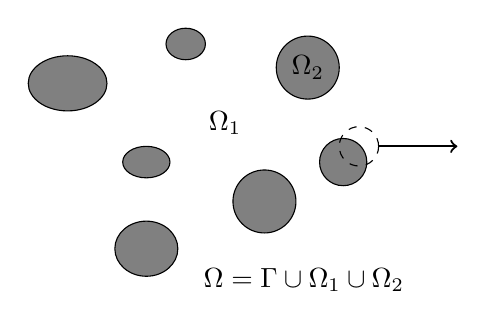
\begin{tikzpicture}
        \foreach \x/\y/\ra/\r in {
        1/3/0.2/0.25,
        2.55/2.7/0.4/0.4,
        0.5/0.4/0.35/0.4,
        2/1/0.4/0.4,
        3/1.5/0.3/0.3,
        0.5/1.5/0.2/0.3,
        -0.5/2.5/0.35/0.5}{
            \draw[fill=gray](\x,\y) ellipse(\r cm and \ra cm);
        }
        \draw[dashed](3.2,1.7)circle(0.25);
        % \draw[thick,->](3.2,1.7)++(0.1767,0.1767)--++(0.4,0.4)--++(1,0);
        \draw[thick,->](3.2,1.7)++(0.25,0)--++(1,0);
        \draw(2.55,2.7)node{$\Omega_2$};
        \draw(1.5,2)node{$\Omega_1$};
        \draw(2.5,0)node{$\Omega = \Gamma \cup \Omega_1 \cup \Omega_2$};
        % \draw(2.5,-1)node{$\Gamma = \sum_\alpha \Gamma_\alpha$};
        % \draw(2.5,-0.5)node{$\Omega_2 = \sum_\alpha \Omega_\alpha$};
    \end{tikzpicture}
    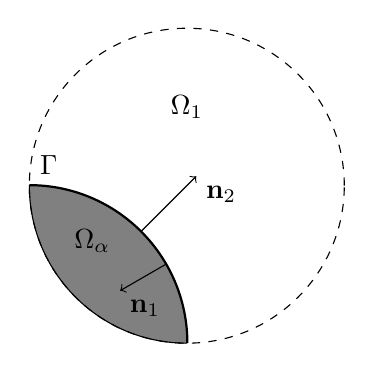
\begin{tikzpicture}%[scale = 0.9]
        \draw[very thick](0:2)arc(0:90:2)node[above right]{$\Gamma$};
        \draw[fill=gray](0:2)arc(0:90:2)arc(180:270:2);
        \draw[dashed](2,2)circle(2);
        \draw[->](1.42,1.42)--++(0.7,0.7)node[below right]{$\textbf{n}_2$};
        \draw[->](1.73,1)--++(-0.577,-0.333)node[below right]{$\textbf{n}_1$};
        \draw(2,3)node{$\Omega_1$};
        \draw(0.8,1.3)node{$\Omega_\alpha$};
    \end{tikzpicture}
    \caption{Topology of dispersed two-phase flows.}%Domain definitions and scheme of the topology of dispersed two-phase flows.}
    \label{fig:Scheme}
\end{figure}

We consider a system consisting of two phases, separated by a sharp interface $\Gamma(t)$ which evolves over time. 
For further insights into the modeling of sharp interface thermodynamics, a comprehensive review may be found in \cite{bothe2022sharp}. 
Each phase subdomain is denoted as $\Omega_1(t)$ and $\Omega_2(t)$, representing the continuous phase (1) and the dispersed phase (2) respectively (refer to Figure \ref{fig:Scheme}).
The entire domain, denoted as $\Omega$, is defined as the union of $\Omega_1$, $\Omega_2$, and $\Gamma$.
To track the position of the phase indexed $k$ and the interfaces, we introduce the phase indicator function $\chi _k$ defined as
\begin{align}
    \chi_k(\textbf{x},t) =  \left\{
      \begin{tabular}{cc}
        $1 \;\text{if} \;\textbf{x} \in \Omega_k(t)$\\
        $0 \;\text{if} \;\textbf{x} \notin \Omega_k(t)$
      \end{tabular}
      \right.
      \text{for $k = 1,2$}.
      \label{eq:PIF}
\end{align}


\subsection{Topological equations}
Using the distribution formalism, one may show that $\chi_k$ obeys the following relations \citep{drew1983mathematical,orlando2023evolution}. 
\begin{align}
    \pddt \chi_k
    + \textbf{u}_I^0 \cdot \grad \chi_k
    &= 0,
    \label{eq:dt_chi_k}\\
    \label{eq:grad_chi_k}
    \grad \chi_k
    &= - \delta_I \textbf{n}_k. 
\end{align}
where $u^0_I$ is the velocity of the interface and $\delta_I$ is the Dirac function localized on the interface.
Then, to describe the evolution of $\delta_I$ we take the gradient for \ref{eq:dt_chi_k} and the gradient of \ref{eq:grad_chi_k} which yields two equations of the interface indicator function \citep{marle1982macroscopic,morel2007surface,orlando2023evolution},
\begin{align}
    \pddt \delta_I
    + \div (\delta_I (\textbf{u}_I^0\cdot \textbf{n}) \textbf{n})
    &= \delta_I (\textbf{u}_I^0 \cdot \textbf{n})(\div\textbf{n})
    \label{eq:dt_delta_I}\\
    \grad\delta_I 
    &= \textbf{n} \cdot \grad (\textbf{n} \delta_I),
    \label{eq:grad_delta_I}
\end{align}
Notice that only the normal components of the surface velocity plays a role in this equation. 
We also employ the subscript $_I$ to indicate any quantity inherently defined on the interface such as its local velocity $\textbf{u}_I^0$. 

\ref{eq:dt_chi_k}, \ref{eq:dt_delta_I}, \ref{eq:grad_delta_I} and \ref{eq:grad_chi_k} are commonly referred to as the topological equations. 
It describes the evolution in space and time of the topology of the flow interfaces.
To enhance clarity, we will omit the time and position parameters from $\chi_k(\textbf{x},t)$ and $\delta_I(\textbf{x},t)$ in the subsequent sections.

\subsection{Local conservation equations}
\label{sec:local_eq}
Let now introduce the local conservation laws that govern the fluid inside bulk phases and the interfaces. 

\subsubsection{Inside the volumes}

Within phase $k$, we note $\rho_k$ the density, $\textbf{u}_k^0$ the local velocity and $E_k^0$ the local total energy per units of mass.
All over the domain $\Omega_k(t)$ the mass, momentum and total energy obey these conservation laws :
\begin{align}
    \label{eq:dt_rho}
    \pddt \rho_k  
    + \div (
        \rho_k\textbf{u}_k^0
    )
    &= 
    0\\
    \label{eq:dt_rhou_k}
    \pddt (\rho_k\textbf{u}_k^0)  
    + \div (
        \rho_k\textbf{u}_k^0\textbf{u}_k^0
        - \bm{\sigma}_k^0 
    )
    &= 
    \rho_k \textbf{g}\\
    \label{eq:dt_rhoE_k}
    \pddt (\rho_kE_k^0)  
    + \div (
        \rho_kE_k^0\textbf{u}_k^0
        + \textbf{q}_k^0
        - \textbf{u}_k^0 \cdot \bm{\sigma}_k^0 
        )
    &= 
    \textbf{u}_k^0 \cdot \textbf{g}  \rho_k
\end{align} 
All along this work the continuous phase will be considered as Newtonian fluid thus, $\bm{\sigma}_1^0 = - p_1^0 \bm\delta + \bm{\tau}_1^0$ where $\bm{\tau}_1^0$ is the Newtonian stress tensor with $p_1 ^0$ the local pressure and $\bm{\tau}_1^0 = \mu_1[\grad \textbf{u}_1^0+(\grad \textbf{u}_1^0)^T]$ the shear rate. 
The vector $\textbf{q}_k^0$ represent the thermal energy flux and is often model with a Fourier law : $\textbf{q}_k^0 = -\lambda \grad T_k^0$ where $T_k$ is the temperature and $\textbf{g}$ is the acceleration of gravity which will be the only body force in the present problem. 
All along this work the superscript $^0$ indicate that the variable is defied at the local or microscopic scale, in opposition to the averaged or macroscopic quantities that will be presented latter. 

The total energy is decomposed in the usual way, i.e. $E_k^0 = e_k^0 + (u_k^0)^2/2$ where  $e_k^0$ is the internal energy which represent the molecular agitation and $(u_k^0)^2/2$ is the kinetic energy per unit of mass.
This decomposition and the previous set of equations lead us to two independent equations for $e_k$ and $u_k$, namely,
\begin{align}
    \label{eq:dt_rhou_k2}
    \pddt [\rho_k(u_k^0)^2]  
    + \div [\rho_k(u_k^0)^2\textbf{u}_k^0/2 - \textbf{u}_k^0 \cdot \bm{\sigma}_k^0]
    &=
    \rho_k\textbf{u}_2^0 \cdot \textbf{g}  
    -  \bm{\sigma}_k^0 : \grad \textbf{u}_k^0,
    \\
    \label{eq:dt_rhoe_k}
    \pddt (\rho_ke_k^0)  
    + \div (
        \rho_ke_k^0\textbf{u}_k^0
        + \textbf{q}_k^0
        )
    &= 
    \bm{\sigma}_k^0 : \grad \textbf{u}_k^0. 
\end{align} 
We can observe that the viscous dissipation term, $\bm{\sigma}_k^0 : \grad \textbf{u}_k^0$,  appears with opposite sign in both of the above equations.
This indicates that $\bm{\sigma}_k^0 : \grad \textbf{u}_k^0$ is the energy that is transformed from kinetic to internal energy. 
By the use of thermodynamics equilibrium laws one can show that from the internal energy equation one can derive an equation for the local temperature \citet{ishii2010thermo}.
In this work we display the internal energy equation for completeness, no link with the temperature or any other thermodynamic quantity will be given. 
We will rather focus on the fluid and particle kinetic energy. 

\subsubsection{On interfaces}

\tb{
    dans cette section il y a une petite incoherence sur les equation energetique de surface. 
    En fait $E_I^0 = e_I^0 + (u_I^0)^2$ avec $e_I$ energie iinerne de surface qui est liée a la tension de surface par $\gamma = e_I − T_I s_I$ avec $T$ la temperature et $s$ l'entropie. bref faut que je mette tout ca au claire. 
    Pour résoudre le pbl voir\cite{ishii2010thermo}
}

On the interface $\Gamma(t)$ the conservation laws take the form of $2d$ conservation laws due to the topology of the interface. 
They are often viewed as \textit{jump condition} which make the link between the conservation equations in both phases. 
The interface mass and momentum conservation equation are well established.
However, the energy conservation law jump condition at the interface is less employed.
In the most general case the mass, momentum and energy surface equations can be written as\citep{morel2015mathematical}, 
\begin{align}
    \label{eq:dt_rhoI}
    \pddt \rho_I
    + \rho_I (\textbf{u}_I^0 \cdot \textbf{n})(\div \textbf{n})
    + \divI (\rho_I\textbf{u}_{I||}^0)
    &= 
    0
    % \Jump{
    %     \rho_k (\textbf{u}_I - \textbf{u}_k)
        % \mathbf{T}_k
    % }
    \\
    \label{eq:dt_rhoIu_I}
    \pddt (\rho_I\textbf{u}_I^0)  
    + \rho_I \textbf{u}_I^0 (\textbf{u}_I^0 \cdot \textbf{n})(\div \textbf{n})
    + \divI (
    \rho_I\textbf{u}_I^0\textbf{u}_{I||}^0
    - \bm{\sigma}_{I||}^0)
    &= 
    \rho_I \textbf{g}
    - \Jump{
        % \rho_k \textbf{u}_k (\textbf{u}_I - \textbf{u}_k)
        \bm\sigma^0_k
    }\\
    \label{eq:dt_rhoIE_I}
    \pddt (\rho_IE_I^0)  
    + \rho_IE_I^0  (\textbf{u}_I \cdot \textbf{n})(\div \textbf{n})
    + \divI (
        \rho_I E_I^0\textbf{u}_{I||}^0
        - \textbf{u}_I^0 \cdot \bm{\sigma}_I^0 
        + \textbf{q}_{I||}^0
        )
    &= 
    \textbf{u}_k^0 \cdot \textbf{g}  \rho_I
    - \Jump{\textbf{u}_k^0 \cdot \bm{\sigma}_k^0 - \textbf{q}_k^0}
\end{align} 
where, $\rho_I$ is the mass per unit of surface of the interface, $\textbf{u}_I^0$ is the local velocity of the interface $\Gamma(t)$, $\bm{\sigma}_I^0$ is the local momentum diffusive flux of surface, $\textbf{q}_I^0$ is the local internal energy diffusive flux of surface and $E_I^0 = e_I^0 + \frac{1}{2}(u_I^0)^2$ is the total energy at the interface, with $e_I^0$ the interface internal energy. 
We introduced the surface divergence operator defined as $\divI ()= (\bm\delta-\textbf{nn})\cdot \div ()$, which correspond to the divergence operator projected on $\Gamma(t)$. 
Throughout this work we use the subscript  $_{||}$ to indicate the projection of a quantity onto the plane tangential to the surface $\Gamma(t)$. 
Specifically, for an arbitrary quantity $\textbf{f}$ defined on $\Gamma(t)$, we denote its tangential projection as $\textbf{f}_{||}^0 = (\bm\delta-\textbf{nn})\cdot \textbf{f}^0$. 
Notice that the diffusive flux $\bm{\sigma}_{I||}^0$ and $\textbf{q}_{I||}^0$ appear as quantity projected on the surface tangential plane.
Indeed, it can be shown that only the tangential parts of the diffusive flux plays a role in the surface momentum balance equations, see \citet{slattery2007interfacial}.
We also introduced the notation $\Jump{\ldots}$, which is defined as $\Jump{\ldots} = \sum_{k=1}^2 [\ldots] \cdot \textbf{n}_k$.
Where $\textbf{n}_k$ is the outward normal vector associated with the domain $\Omega_k$ (see \ref{fig:Scheme}).

The formulations given by \ref{eq:dt_rho_I},\ref{eq:dt_rhoIu_I}and \ref{eq:dt_rhoI} remains quite general and needs some further simplifications. 
First we assume a thermodynamic local equilibrium everywhere at the interfaces. 
In this case the interfacial energy is closely related to the surface tension coefficient noted $\gamma$, that will be considered constant throughout this work. 
We assume that the momentum diffusive flux of surface is solely due to surface tension, therefore $\bm{\sigma}_I^0  = \gamma (\bm\delta - \textbf{nn}) = \gamma \bm\delta_{||}$ where $\gamma$ is the surface tension coefficient which will be assumed constant overall the interfaces \citep[Chapter 2]{tryggvason2011direct}.  
Note that in a more general case, interfacial viscous stress could be included into $\bm{\sigma}_{I}^0$ \citep{brenner2013interfacial,slattery2007interfacial,nadim1996concise}, nevertheless it will not be addressed in this study. 
Additionally, we assume the surface density to be negligible thus $\rho_I = 0$ and since we considered no energy accumulation at the interface $\textbf{q}_I=0$.
Also, instead of 
Consequently, the interfacial mass, momentum and total energy balance equations reduce to the common expressions :
\begin{align}
    \label{eq:dt_rho_I}
    \Jump{
        \rho_k (\textbf{u}_I - \textbf{u}_k)
        % \mathbf{T}_k
    }
    &=0, \\
    \Jump{\bm{\sigma}_k^0} 
    &=
    \divI\bm\sigma^0_{I||}
    =
    -\gamma\textbf{n}(\div \textbf{n}),
    % + \gradI\sigma 
    \label{eq:surface_tension}\\
    \label{eq:dt_rhoI_EI}
    - \Jump{\textbf{u}_k^0 \cdot \bm{\sigma}_k^0 - \textbf{q}_k^0}
    &=
    \pddt \gamma + \divI(\gamma \textbf{u}_I - \bm\sigma^0_{I||}\cdot \textbf{u}_I^0 )
    =
    + \gamma\textbf{n}\cdot \textbf{u}_{I}^0(\div \textbf{n}),
    % +
    % \label{eq:dt_rhoIe_I}
    % \Jump{ \textbf{q}_k^0}eq:dt_rho_I
    % &= 
    %  0
\end{align}
respectively. 
Where $ - \div\textbf{n}$ is twice the mean interface curvature.
% In \ref{eq:surface_tension}, we can clearly identify two contributions : the first one related to the curvature, and the second one from the non-constant surface tension coefficient along the surface. 
% The latter contribution is responsible for the Marangonie effect.
% This terms 
\ref{eq:dt_rhoI_EI} is the jump equation for the total energy.
However, in the following it will be more practical to deal with an equation for the kinetic and internal energy separately. 
Thus, we take the dot product of \ref{eq:surface_derivative}, \ref{eq:} with $\textbf{u}_I$ and subtract this new expression to \ref{eq:dt_rhoI_EI} which gives us, 
\begin{align}
    \label{eq:dt_rhoI_uI2}
    \Jump{\textbf{u}_k^0 \cdot \bm{\sigma}_k^0}
    &=
    -\gamma\textbf{n}\cdot \textbf{u}_{I}^0(\div \textbf{n})\\
    \label{eq:dt_rhoIe_I}
    \Jump{ \textbf{q}_k^0}
    &= 
     0
\end{align}
for the interface kinetic energy and the internal interface energy, respectively. 
Notice that this decomposition is possible only under the assumption of no mass transfer in which case $\textbf{u}_I^0=\textbf{u}_k^0$ for $k =1,2$ and a constant surface tension coefficient.


In the perspective of ensemble averaging the objective of the next two subsections is to extend the domain of definition of these two equations to the whole space $\Omega$.


\subsubsection{Generic formulation}

For ease of understanding, we now introduce generic conservation laws in the volumes and on the interfaces. 
Let $f_k^0(\textbf{x},t)$ denote a volumetric quantity of arbitrary tensorial order defined in $\Omega_k(t)$.
Likewise, let $f_I^0(\textbf{x}_I,I)$ represent an arbitrary surface property defined on $\Gamma(t)$.
Using the strategy outlined in \citep{bothe2022sharp,morel2015mathematical,slattery2007interfacial}, we can derive the local conservation equations for both $f_k^0(\textbf{x},t)$ and $f_I^0(\textbf{x}_I,t)$, that is,  
\begin{align}
    \label{eq:dt_f_k}
    \pddt f_k^0
    +\div \left(
        f_k^0\textbf{u}_k^0
        - \mathbf{\Phi}_k^0
        \right)
    &= 
    s_k^0
    & \text{ in } \Omega_k(t),&\\
    \pddt f_I^0 
    + f_I^0 (\textbf{u}_I \cdot \textbf{n})(\div \textbf{n})
    +\divI
    (f_I^0 \textbf{u}_{I||}^0
        - \mathbf{\Phi}_{I||}^0 )
    &= 
    s_I^0
    - \Jump{
       f_k (\textbf{u}_I^0 - \textbf{u}_k^0)
       + \mathbf{\Phi}_k^0
    } 
    & \text{ on } \Gamma(t),&
    \label{eq:dt_f_I}
\end{align}
respectively.
The tensors $\mathbf{\Phi}_k^0(f_k)$ and $\mathbf{\Phi}_{I||}^0(f_I)$ represent the non-convective fluxes corresponding to $f_k^0$ and $f_I^0$. 
Notice that $\mathbf{\Phi}_{I||}^0$ also carries the $_{||}$ subscript which implies that only the tangential component of this tensor remain in the surface balance equation. 
Similarly, $s_k^0(f_k^0)$ and $s_I^0(f_I^0)$ represent the source terms of $f_k^0$ and $f_I^0$, respectively.
Notice, that in \ref{eq:dt_f_I} we kept the mass transfer term $f_k (\textbf{u}_I^0 - \textbf{u}_k^0)$ for purpose of generality. 
For practical uses, note that the advecting term in \ref{eq:dt_f_I}can be written in the more compact form $f_I^0 (\textbf{u}_I \cdot \textbf{n})(\div \textbf{n})
+\divI(f_I^0 \textbf{u}_{I||}^0) = \divI(f_I^0 \textbf{u}_I^0)$ by noticing that $\textbf{n}\cdot\gradI(\ldots) = 0$ and $\divI\textbf{n} = \div\textbf{n}$ \citep{nadim1996concise}.
It is important to note that \ref{eq:dt_f_k} and \ref{eq:dt_f_I} are solely defined within $\Omega_k(t)$ and $\Gamma(t)$, respectively.
This was also the case for the equations presented in the last two subsections. 
Consequently, these equations are referred to as local conservation equations. 


\subsection{The two-fluid formulation}
The presence function $\chi_k$, and the Dirac delta function $\delta_I$, allow the extension of local conservation equations to the entire flow domain $\Omega$. 
This extension is achieved by employing the methodology introduced by \citet{drew1983mathematical} and \citet{kataoka1986local} for the conseriving laws inside the volume (\ref{eq:dt_f_k}).
For any local quantities $f_k^0$ defined in $\Omega_k(t)$, we assign the field $\chi_k f_k^0$, which is defined over the entire domain $\Omega$. The two-fluid formulation may be obtained by multiplying \ref{eq:dt_f_k} by $\chi_k$. 
Using \ref{eq:dt_chi_k} and \ref{eq:grad_chi_k} we obtain
\begin{equation}
    \pddt (\chi_k f_k^0)
    + \div (
        \chi_k f_k^0 \textbf{u}_k^0
        - \chi_k \mathbf{\Phi}_k^0 
        )
    = 
    \chi_k s_k^0
    + \delta_I\left[
        f_k^0
        \left(
            \textbf{u}_I^0
            - \textbf{u}_k^0
        \right)
        + \mathbf{\Phi}_k^0
    \right]
    \cdot \textbf{n}_k.
    \label{eq:dt_chi_k_f_k}
\end{equation}
Likewise, for any surface property $f_I^0$ defined on $\Gamma(t)$, we assign the field $\delta_I f_I^0$, which is also defined all over $\Omega$. 
Following the approach outlined \citet[Appendix 2]{marle1982macroscopic} we can generalize \ref{eq:dt_f_I} to the 3D space. 
Making use of the topological equations \ref{eq:dt_delta_I} and \ref{eq:grad_delta_I} gives,
\begin{equation}
    \pddt (\delta_If_I^0)  
    + \div (
        \delta_I f_I^0 \textbf{u}_I^0
        - \delta_I \mathbf{\Phi}_{I||}^0 
        )
    = 
    \delta_Is_I^0
    - \delta_I\Jump{
    f_k^0 (\textbf{u}_I^0 - \textbf{u}_k^0)
    + \mathbf{\Phi}_k^0} 
    \label{eq:dt_delta_I_f_I}
\end{equation}
which correspond to the conservation equation for $\delta_If_I^0$.
The last term on the right hands side of \ref{eq:dt_chi_k_f_k} represent the phase transfer of $f_k$ across the interfaces and the non-convective fluxes across phases.
The set of equations formed by \ref{eq:dt_chi_k_f_k} for $k =1,2$ is commonly known as the \textit{two-fluid} formulation of multiphase flows, to which we add the \textit{jump condition} across the phase given by \ref{eq:dt_delta_I_f_I} \citep{morel2015mathematical,tryggvason2011direct,drew1983mathematical,kataoka1986local}. 

\tb{this formulation is useful for the bulk stress}
In this work, we prefer to think of those equations as a set of three equations formed by \ref{eq:dt_chi_k_f_k} for $k=1,2$ and \ref{eq:dt_delta_I_f_I}. 
We define the \textit{bulk} property $\textbf{f}$ as $\textbf{f}^0 = \sum_k \chi_k \textbf{f}_k^0 + \delta_I \textbf{f}_I^0$ where $\textbf{f}^0$ represents any property of the flow of arbitrary tensorial order at the local scale.
Then by summing \ref{eq:dt_chi_k_f_k} for $k=1,2$ and \ref{eq:dt_delta_I_f_I}, one obtain the \textit{single-fluid} formulation conservation equation, namely,
\begin{equation}
   \pddt f^0
   + \div (
       f^0 \textbf{u}^0
       -  \mathbf{\Phi}^0 
    )
   = s^0. 
   \label{eq:dt_f}
\end{equation}
It should be noted that in the literature we rather define the \textit{bulk} quantities as $f^0 = \sum_k \chi_k f_k^0$, while the interfacial component is treated as a source term in \ref{eq:dt_f} \citep{morel2015mathematical,tryggvason2011direct,drew1983mathematical}. 
Nevertheless, we want to point out here that with this definition we recover a classic transport equation for the bulk quantity $f^0$ which makes the whole system of equation consistent.




\subsection{The averaged conservation equations}
In this study, we employ the ensemble average technique to establish the averaged conservation equations. 
This method is just one of several averaging approaches, including the volume average method \citep{jackson1997locally} and time averaging \citep{ishii2010thermo}. 
Despite their differences, all these techniques yield the same set of averaged equations \citep{jackson1997locally,zhang1997momentum}.
In the following we recall some properties of the ensemble average operator. 
Let, $P(\FF)$ be the probability density function that describe the probability of finding the flow in the configuration $\FF$. 
It follows from this definition, that the ensemble average of an arbitrary local property $f^0(\textbf{x},t;\FF)$ defined on the whole space $\Omega$, is,
\begin{equation}
    f(\textbf{x},t)
    = \avg{f^0}(\textbf{x},t)
    =\int f^0(\textbf{x},t;\FF) d\mathscr{P}. 
    \label{eq:avg}
\end{equation}  
Note that we dropped the super script $^0$ on $f$ to indicate that this is an averaged quantity. 
Therefore, all variables denoted with a $^0$ are functions of $(\textbf{x}, t; \FF)$, whereas all macroscopic variables are averaged over all $\FF$ and thus depend only on $(\textbf{x}, t)$.
The ensemble average quantities are assumed to satisfy the following properties \citep{drew1983mathematical}
\begin{align}
    \avg{f^0+h^0} &= f+h, \\ 
    \avg{\avg{f^0}h^0} &= fh, \\
    \avg{\pddt f^0} 
    &= \pddt f, \\ 
    \avg{\grad f^0}
    &= \grad f. 
    \label{eq:avg_properties}
\end{align}
were $f$ and $h$ are two arbitrary Eulerian fields. The first two relations are called the Reynolds' rules, the third one is the Leibniz' rule and the last one, the Gauss' rule \citep{drew1983mathematical}.
Additionally, for any phase quantity defined in $\Omega_k$ we introduce the definition, 
\begin{equation}
    \phi_k f_k (\textbf{x},t) = \avg{\chi_k f_k^0}
    \label{eq:1_avg}
\end{equation}
where, $\phi_k(\textbf{x},t) = \avg{\chi_k}$ is the volume fraction of the phase $k$
and $f_k(\textbf{x},t)$ the average of the field $f_k^0$ conditioned on the presence of the phase $k$ at $\textbf{x}$ and time $t$.
Equally, for interface quantities we have 
\begin{equation}
    \phi_I f_I (\textbf{x},t) = \avg{\delta_I f_I^0}
\end{equation}
with $\phi_I = \avg{\delta_I}$ the interfacial area concentration function and $f_I(\textbf{x},t)$ the average of $f^0_I(\textbf{x},t,\FF)$ conditioned on the presence of an interface at $\textbf{x}$ and time $t$. 
The fluctuation of a phase-averaged quantity around its mean is defined by,
\begin{align}
    f_k' = f_k^0 - f_k.
    && f_I' = f_I^0 - f_I.
    \label{eq:def_fluctu}
\end{align}
Thus, the product $\avg{\chi_k f^0_kg^0_k}$ can be decomposed as $\avg{\chi_k f_k^0g_k^0}=\phi_k f_kg_k + \avg{\chi_k f'_kg'_k}$. 


Applying the ensemble average on \ref{eq:dt_chi_k_f_k} and \ref{eq:dt_delta_I_f_I} and considering the properties from \ref{eq:avg_properties} together with \ref{eq:def_fluctu} yields the general form of the averaged equations of multiphase flows, namely,
\begin{align}
    \pddt (\phi_k f_k)
    +\div (\phi_k f_k \textbf{u}_k - \mathbf{\Phi}_k^\text{eq})
    &= 
    \phi_k s_k
    + \avg{\delta_I\left[
        \mathbf{\Phi}_k^0
        + f_k^0
        \left(
            \textbf{u}_I^0
            - \textbf{u}_k^0
        \right)
    \right]
    \cdot \textbf{n}_k} ,
    \label{eq:avg_dt_chi_f}\\
    \pddt (\phi_I f_I)
    +\div (\phi_I f_I \textbf{u}_I- \mathbf{\Phi}_{I}^\text{eq})
    &= 
    \phi_I s_I
    - \avg{\delta_I 
    \Jump{
    f_k^0 (\textbf{u}_I^0 - \textbf{u}_k^0)
    + \mathbf{\Phi}_k^0
    } 
     }.
    \label{eq:avg_dt_delta_f}
\end{align}
where $\mathbf{\Phi}_{I}^\text{eq}$ and $\mathbf{\Phi}_{I}^\text{eq}$ are the equivalent non-convective fluxes defined as 
\begin{align*}
    \mathbf{\Phi}_k^\text{eq}
    = \avg{\chi_k f_k' \textbf{u}_k'}
    - \phi_k \bm\Phi_k,
    &&
    \mathbf{\Phi}_{I}^\text{eq}
    = \avg{\delta_I f_I' \textbf{u}_I'}
    - \phi_I \bm\Phi_I. 
\end{align*}
% Note that while all terms are just the average of their local counterpart, the covariance term $\avg{\chi_k f_k' \textbf{u}_k'}$ and $\avg{\delta_I f_I' \textbf{u}_I'}$ arise fropurely mathematical 
These equations are to be solved for the averaged field $\phi_k,\phi_I,f_k$ and $f_I$ with a complementary equation of volume conservation, i.e. $\phi_1+\phi_2+\phi_I w_I = 1$ where $w_I$ is the mean width of the interfaces.
% Thus, all term in these equations must be expressed as a function of $\phi_k,\phi_I,f_k$ and $f_I$. 
The main differences between these equations and their microscale counterparts (\ref{eq:dt_f_k} and \ref{eq:dt_f_I}) are:
(1) The unknowns are averaged quantities,
(2) Factors $\phi_k$ and $\phi_I$ are introduced in front of all the terms, and
(3) The additional stresses $\avg{\chi_k f_k' \textbf{u}_k'}$ and $\avg{\delta_I f_I' \textbf{u}_I'}$ appear, representing the covariance between the conserved quantity and the local velocities.  
For a complete understanding, we derived the mass, momentum, and energy averaged equations in \ref{ap:two-fluid_model}. 
Especially we demonstrate how to derive the secondary equations of the averaged energy $E_k$, i.e. the equation for the mean internal energy $e_k$, the pseudo turbulent energy (defined therein) and the averaged kinetic energy $(u_k)^2/2$.  

It is important to highlight that the two-fluid model fails to adequately distinguish between the two phases, as evidenced by the \textit{symmetry} $k = 1$ and $2$ in the aforementioned equations. This symmetry does not hold physically because the dispersed phase possesses a distinct topological nature compared to the continuous phase. 
More importantly, in a dispersed two phase flow system the closure terms are expressed as a function of the Lagrangian properties of the particles whereas this system of equation provides us with continuously averaged quantities. 
Specifically, the mean drag force term in the averaged momentum equation is expressed as a function of the  center of mass velocity of the particles. 
Whereas this system of equation provides us with the phase averaged velocity of the whole phase not with no consideration for the center of mass.  
Therefore, in the subsequent section, we will introduce a kinetic model specifically devoted to the dispersed phase. 
As illustrated below, the equations governing the dispersed phase are more comprehensive as they bear a resemblance to the equations governing a single particle.





While \ref{eq:dt_chi_k_f_k} and \ref{eq:dt_delta_I_f_I} describe multiphase-flow in a general manner, they do not leverage the topology of the dispersed phase. 
Therefore, in this section, we present a Lagrangian-based model capable of describing the dispersed phase with an arbitrary order of accuracy.

\subsection{Fundamental properties}

At this stage, it is crucial to define some fundamental properties associated to each particle.
Following the strategy of \citet{lhuillier2009rheology,lhuillier1992volume,zaepffel2011modelisation} and \citet[Chapter 2]{morel2015mathematical}
we define the mass, position of center of mass, momentum and total energy of the particle $\alpha$, such as,
\begin{align}
    &m_\alpha(t)
    = \int_{\Omega_\alpha(t)} \rho_2  d\Omega,
    % &&
    &\textbf{x}_\alpha(t)
    = \frac{1}{m_\alpha(t) }\int_{\Omega_\alpha(t)} \rho_2 \textbf{x} d\Omega,\\
    % &&
    &\textbf{p}_\alpha(t) 
    = \int_{\Omega_\alpha(t)} \rho_2 \textbf{u}_2^0 d\Omega,
    % &&
    & m_\alpha E_\alpha(t) 
    = \int_{\Omega_\alpha(t)} \rho_2 [e_2^0 + (u_2^0)^2/2] d\Omega,
    \label{eq:position_and_momentum_def}
\end{align}
respectively. 
Where $\Omega_\alpha$ is the domain occupied by the particle $\alpha$ (see \ref{fig:Scheme}). 
Subsequently, we define the velocity of the particle's center of mass, denoted as $\textbf{u}_\alpha$ which is given by $\textbf{u}_\alpha = \ddt \textbf{x}_\alpha$. 
The derivation of $\ddt \textbf{x}_\alpha$ is straightforward but requires some algebra which are detailed in \ref{ap:velocity_definition}. 
The final expression reads,
\begin{equation}
    \textbf{u}_\alpha(t) = \frac{1}{m_\alpha(t)} \left(
        \textbf{p}_\alpha(t)
        +  \int_{\Sigma_\alpha(t)} \rho_2 \textbf{r} (\textbf{u}_I^0 - \textbf{u}_2^0)\cdot \textbf{n}_2 d\Sigma
        \right),
        \label{eq:dt_y_alpha}
\end{equation}
where $\textbf{r}(\textbf{x},t) = \textbf{x} - \textbf{x}_\alpha(t)$. 
In Equation \ref{eq:dt_y_alpha}, it can be observed that the first component of the velocity represents the linear momentum divided by the mass of the particle. 
This corresponds to the mass-averaged velocity over the volume of the particle.
The second term in Equation \ref{eq:dt_y_alpha} arises from the contribution of anisotropic mass transfer across the surface of the particle. 
This mass transfer leads to the motion of the particle's center of mass, thereby contributing to the total velocity.
To illustrate this concept, let us consider a fixed drop with no momentum lying over a very hot plate.
In this scenario, we assume that the plate is sufficiently hot to induce evaporation, specifically on the bottom portion of the drop.
Hence, under the effect of an anisotropic evaporation flux one may expect the second term to be non-negligible.
Consequently, the center of mass of the drop has a non-zero velocity in the opposite direction of the plate, even though the momentum is assumed to be zero.
We can also consider the case of the nucleation of a bubble in water. 
In this case, although the particle momentum is null at all time the center of mass of the particle moves due to the growth of the particle. 
In both cases, we need to take into account the mass transfer term in \ref{eq:dt_y_alpha}, while the first term is negligible. 
Note that \ref{eq:dt_y_alpha} generalized usual expression of the center of mass velocity whom neglect the second term.
In the following, we discard the time dependency notation for all Lagrangian quantities denoted by the subscript $_\alpha$ and also $\Sigma(t)$ and $\Omega_\alpha$.
Nevertheless, the reader must understand that all Lagrangian quantities and integration domains subscribed by $_\alpha$ are time dependent. 

The particle's internal relative motions or the \textit{inner velocity} is given by $\textbf{w}_2^0(\textbf{x},t) = \textbf{u}_2^0(\textbf{x}) - \textbf{u}_\alpha(t)$.
Thus, from its definition in \ref{eq:position_and_momentum_def}, we can rewrite the momentum as follows,
\begin{equation}
    \label{eq:momentum_definition_1}
    \textbf{p}_\alpha
    = m_\alpha \textbf{u}_\alpha
    + \int_{\Omega_\alpha} \rho_2 \textbf{w}_2^0 d\Omega.
\end{equation}
Alternatively, by manipulating \ref{eq:dt_y_alpha}, we obtain,
\begin{equation}
    \textbf{p}_\alpha
    =  m_\alpha \textbf{u}_\alpha
    - \int_{\Sigma_\alpha} \rho_2\textbf{r}(\textbf{u}_I^0 - \textbf{u}_2^0)\cdot \textbf{n}_2 d\Sigma
    \label{eq:momentum_definition}
\end{equation}
Therefore, the momentum of a particle can be seen as a sum of the mean velocity plus the integral of the fluctuation (\ref{eq:momentum_definition_1}), with the latter being equivalent to minus the first moment of mass transfer term (\ref{eq:momentum_definition}).
Indeed, by identification we obtain : $\int_{\Omega_\alpha} \rho_2 \textbf{w}_2^0 d\Omega =\int_{\Sigma_\alpha}  \rho_2\textbf{r} (\textbf{u}_I^0 - \textbf{u}_2^0)\cdot \textbf{n}_2 d\Sigma$. 
The essential aspect of this relation highlighted here is that the internal velocity fluctuations within a fluid particle do not contribute to the total linear momentum $\textbf{p}_\alpha$, as long as the anisotropic mass transfer is negligible.  
Additionally, the total energy $E_\alpha$ can be decomposed following a similar procedure which leads us to, 
\begin{equation*}
    \label{eq:E_alpha_def}
    m_\alpha E_\alpha(t) 
    = m_\alpha e_\alpha 
    + W_\alpha
    + m_\alpha (u_\alpha)^2/2
    % + \textbf{u}_\alpha \cdot \int_{\Omega_\alpha(t)} \rho_2  \textbf{w}_2^0 d\Omega
\end{equation*}
where we introduced the internal kinetic energy : $W_\alpha = \int_{\Omega_\alpha(t)} \rho_2  (w_2^0)^2/2 d\Omega$. 
In that expression mass transfer have been neglected. 
Anyhow, the total energy of a particle is the sum of its internal energy $e_\alpha$, internal kinetic energy $W_\alpha$ and the kinetic energy  due to its own center of mass displacement $u_\alpha^2/2$. 
To gain in understanding, let's express $W_\alpha$ in the case of a solid particle.
The velocity inside a solid particle can be expressed : $\textbf{u}_2^0(\textbf{x}_\alpha + \textbf{r}) = \textbf{u}_\alpha + \textbf{r}\times \bm{\omega}_\alpha$ where $\bm{\omega}_\alpha$ is the angular velocity.  
In this case, $W_\alpha = \bm{\omega}_\alpha\bm{\omega}_\alpha\cdot \mathcal{I}_\alpha$ where $\mathcal{I}_\alpha$ is the inertia matrices of the particle. 
As a matter of facts for solid particles $W_\alpha$ represents the angular kinetic energy for solid particles.
Thus, for particles with fluid internal motion, $W_\alpha$ is just a more general definition of the particle internal kinetic energy. 

\subsection{Conservation laws}
We assign to a particle indexed, $\alpha$, occupying the domain $\Omega_\alpha$ (see \ref{fig:Scheme}) an arbitrary Lagrangian property $q_\alpha$ defined by $q_\alpha  = \int_{\Omega_\alpha} f_2^0(\textbf{x},t) d\Omega$.
Similarly, we define $q_{I\alpha} = \int_{\Sigma_\alpha} f_I^0(\textbf{x},t) d\Sigma$ as being an integrated surface property associated to the particle $\alpha$.


To describe the evolution of any arbitrary Lagrangian quantity $q_\alpha$, we need to establish its time derivative.
Since, $q_\alpha$ is an integral quantity with a time-dependent domain of integration, we apply the general Reynolds transport theorem for volume integral (exposed in \ref{ap:math}) to compute its time derivative \citep{morel2015mathematical}.
This yields the following expression :
\begin{equation}
    \ddt  q_\alpha
    = \int_{\Omega_\alpha}\left[ \pddt f_2^0 + \div\left(f_2^0\textbf{u}_2^0\right) \right]d\Omega\\
    + \int_{\Sigma_\alpha} f_2^0 (\textbf{u}_I^0-\textbf{u}_2^0)\cdot \textbf{n}_2 d\Sigma.
\end{equation}
By substituting the integrand of the first integral on the right-hand side (RHS) with \ref{eq:dt_f_k} we obtain the conservation laws of the quantity $q_\alpha$, namely,  
\begin{equation}
    \ddt  q_\alpha
    = \int_{\Omega_\alpha} s_2^0 d\Omega
    + \int_{\Sigma_\alpha} \left[
        f_2^0 (\textbf{u}_I^0-\textbf{u}_2^0) 
        + \mathbf{\Phi}_2^0 
        \right] \cdot \textbf{n}_2 d\Sigma,
    \label{eq:dt_q_alpha}
\end{equation}
The first term on the RHS accounts for the total contribution of the source term $s_2^0$ to the particle $\alpha$.
While, The second term on the RHS is the surface integration of the exchange terms, which includes the phase transfer flux $f_2^0 (\textbf{u}_I^0-\textbf{u}_2^0)$ and the diffusive flux $\mathbf{\Phi}_2^0$. 
For clarity, let us consider the specific case of the momentum balance, i.e. when $q_\alpha = \textbf{p}_\alpha$.
In this situation, the first term reads as $\int_{\Omega_\alpha} \rho_2\textbf{g} d\Omega$ and represents the total weight acting on the particle $\alpha$. 
Likewise, the second term represents the total source of momentum due to phase transfer, and it is expressed as, $\int_{\Sigma_\alpha} \rho_2 \textbf{u}_2^0 (\textbf{u}_I^0-\textbf{u}_2^0)\cdot\textbf{n}_2 d\Sigma$. 
Lastly, $\int_{\Sigma_\alpha} \bm{\sigma}_2^0\cdot\textbf{n}_2 d\Sigma$ represents the resultant of the hydrodynamic forces acting on the surface of the particle.
It is important to notice that under this form, the exchange terms are expressed as integrals of dispersed phase fields denoted by the subscript $_2$.
Nevertheless, depending on the nature of the dispersed phase, these fields may not always be defined.
For infinitely rigid particles it is indeed the case since, the stress $\bm{\sigma}_2^0$ isn't defined.  
Hence, our objective is to express these exchange terms, in terms of the continuous phase field quantities instead of the dispersed phase field, i.e. in terms of $\mathbf{\Phi}_1^0$ and $\textbf{u}_1^0$ rather than $\mathbf{\Phi}_2^0$ and $\textbf{u}_2^0$. 

To address this issue, let us derive the conservation equation for the integrated surface property $q_{I\alpha}$.
To differentiate time-varying surface integrals within time, we can use the general Leibniz rule (see \ref{eq:Leibnitz}), to derive the following expression :
\begin{equation}
    \ddt  q_{I\alpha}
    = \int_{\Sigma_\alpha} \left[
        \pddt f_I^0
        +   \gradI \cdot (\textbf{u}_I^0f_I^0)
    \right]d\Sigma.
    \label{eq:surface_derivative}
\end{equation}
Substituting the RHS terms of \ref{eq:surface_derivative} using \ref{eq:dt_f_I}, and making use of the surface divergence theorem on closed surfaces (see \ref{eq:surf_div_theorem}), gives,
\begin{equation}
    \ddt  q_{I\alpha}
    = \int_{\Sigma_\alpha} 
        s_I^0
    d\Sigma
    - \int_{\Sigma_\alpha} \Jump{
        f_k^0 (\textbf{u}_I^0 - \textbf{u}_k^0)
        + \mathbf{\Phi}_k^0
    }
    d\Sigma.
    \label{eq:dt_q_I_alpha}
\end{equation}
This equation can be interpreted as the surface conservation equation for the integrated surface property $f_I$, or as the flux jump condition integrated on a closed surface. 
Notice that $\bm{\Phi}_{I}^0$ isn't present in this balance equation. 
This is due to the fact that as mentioned earlier, only the tangential components of $\bm{\Phi}_{I}^0$ appear inside the surface balance equation, while we perform an integration over a closed surface which is null due to \ref{eq:surf_div_theorem}. 

As discussed above we wish to get rid of $\mathbf{\Phi}_2^0$ in \ref{eq:dt_q_alpha}. To achieve this, we treat the particle's volume and surface as a unified entity and derive a conservation equation for $q_\alpha^\text{tot} = q_\alpha + q_{I\alpha}$. 
This is done by summing \ref{eq:dt_q_alpha} and \ref{eq:dt_q_I_alpha} which leads to, 
\begin{equation}
    \ddt  q_\alpha^\text{tot}
    = 
    \int_{\Omega_\alpha} s_2^0 d\Omega
    + \int_{\Sigma_\alpha} s_I^0 d\Sigma
    + \int_{\Sigma_\alpha} \left[
        f_1^0 (\textbf{u}_I^0-\textbf{u}_1^0) 
        + \mathbf{\Phi}_1^0 
        \right] \cdot \textbf{n}_2 d\Sigma. 
    \label{eq:dt_q_alpha_tot}
\end{equation}
This equation is the general form of the linear conservation law of $\chi_2 f_2^0 + \delta_I f_I^0$ for the system consisting of the particle volume $\Omega_\alpha$, and its surface $\Sigma_\alpha$. It is applicable to any particle immersed into a continuous phase following the local conservation,\ref{eq:dt_f_k} and \ref{eq:dt_f_I}.
We refer to this equation as the zeroth-order conservation equation or the linear conservation law for the particle $\alpha$.

Following the same assumption as in \ref{sec:local_eq}, i.e. we consider no mass transfer and weightless interfaces, the Lagrangian  mass, momentum and energy equations for a single particle can be derived using the generic form \ref{eq:dt_q_alpha_tot} and reads as, 
\begin{align}
    \label{eq:dt_m_alpha}
    \ddt m_\alpha
    &= 
    0\\
    \label{eq:dt_p_alpha}
    \ddt (m_\alpha \textbf{u}_\alpha)
    &= 
    m_\alpha\textbf{g}
    +  \intS{\bm{\sigma}_2^0 \cdot \textbf{n}_2}\\
    \label{eq:dt_E_alpha}
    \ddt (m_\alpha E_\alpha + s_\alpha \gamma)
    &= 
    m_\alpha \textbf{u}_\alpha \cdot \textbf{g}
    +\textbf{u}_\alpha \cdot \intS{\bm{\sigma}_2^0 \cdot \textbf{n}_2}   
    +\intS{\textbf{w}_1^0 \cdot \bm{\sigma}_1^0 \cdot  \textbf{n}_2} 
    - \intS{\textbf{q}_2^0 \cdot \textbf{n}_2}
\end{align}
where  $\int_{\Sigma_\alpha}  \bm{\sigma}_1^0 \cdot \textbf{n}_2 d\Sigma$ is the resultants of the hydrodynamic force and $\int_{\Sigma_\alpha} \textbf{q}_1^0 \cdot \textbf{n}_2 d\Sigma$ is the resultants of the surface heat flux. 
The second term on the right hands side of the energy equation is the work produced by the mean force and the translational motion of the droplets, while $\intS{\textbf{w}_1^0 \cdot \bm{\sigma}_1^0 \cdot  \textbf{n}_2}$ is the work produced by the local forces and local motion of the fluid at the surface of the particle.
Since we integrated the energy over the particle's volume and its surface, we explicitly made appear the surface energy $\gamma s_\alpha$ within the derivative operator. 
Note that these equations does not explicitly account for inter-particle interactions. 
However, it is possible to include manually such forces by noticing that the surface external stress flux $\bm{\sigma}_1^0$ is the sum of hydrodynamic and particles-particles interaction forces, regardless it is pure contact forces from direct contact or a force mediated through the carrier fluid.
From this consideration it is possible to split every term involving the stress $\bm{\sigma}_1^0$ into two terms representing these contributions. 
Same comments can be made for the heat flux $\textbf{q}_1^0$. 
Although this distinction is important, for purpose of clearly we will stay general, and we will keep the fluxes $\bm{\sigma}_1^0$ and $\textbf{q}_1^0$ as such. 

In the spirit of the energy decomposition exposed in \ref{eq:E_alpha_def} the total energy equation can be split into three equations, one for the center of mass kinetic energy, internal motion and internal kinetic energy, namely,  
\begin{align}
    \label{eq:dt_u2_alpha}
    \frac{1}{2}\ddt (m_\alpha u_\alpha^2)
    &= 
    \textbf{u}_\alpha\cdot
    \textbf{g}m_\alpha
    + 
    \textbf{u}_\alpha\cdot
    \textbf{f}_\alpha,\\
    \label{eq:dt_w2_alpha}
    \ddt W_\alpha 
    &= 
    \intS {\textbf{w}_1^0 \cdot \bm{\sigma}_1^0 \cdot \textbf{n}_2 }
    - \intO{ \bm{\sigma}_2^0 : \grad\textbf{u}_2^0 }
    - \ddt (s_\alpha \gamma) 
    \\
     \label{eq:dt_e_alpha}
    \ddt (m_\alpha e_\alpha )
    &= 
     \intO{ \bm{\sigma}_2^0 : \grad\textbf{u}_2^0  }
    -  \intS{\textbf{q}_1^0\cdot \textbf{n}_2 } 
\end{align}
respectively. 
Note that in \citet{eq:dt_w2_alpha} the use of \ref{eq:dt_rhoI_uI2} makes appear explicitly the derivative of the surface energy $s_\alpha \gamma$. 
Note that under this form we see that the energy loss in the deformation represented by $W_p$ will be gathered in the surface energy which will in turn act as a source term in the internal kinetic energy motion.
The surface tension plays the role as a spring in the energy balance.   
From this set of equation we can easily see that the rate of dissipation terms $\intS{\bm{\sigma}_2^0 : \grad\textbf{u}_2^0}$ represent an energy sink in the equation of $W_\alpha$ while it is a source term in the internal energy equation. 
As it has been observed in the previous section, this terms convert the energy of internal motion to molecular agitation. 
However, the interplay between the center of mass  kinetic energy and the internal fluctuation is not obvious and has no common term with the heat and internal kinetic energy equation.
In fact, we will see that the transfer between these scales is archived thought the fluid phase pseudo turbulent energy. 


Finally, we would like to highlight that  due to the consideration of closed surface, the diffusive flux $\mathbf{\Phi}_I$, plays no role at all in \ref{eq:dt_q_alpha_tot}.
Therefore, in the case of the linear momentum conservation law, the contribution of the surface tension forces exposed in \ref{eq:surface_tension}, do not contribute to the momentum balance in \ref{eq:dt_p_alpha}.
As a consequence, even in the presence of local Marangoni forces, the resultant of the local surface tension forces cancels out in the linear momentum balance.
This fact has already been demonstrated by \citet{hesla1993note} who showed that the surface tension force does not contribute to the linear and angular momentum balance. 
Here, we have provided the general proof that the interfacial diffusive flux $\mathbf{\Phi}_I^0$, which is present at the local scale according to \ref{eq:dt_f_I}, does not contribute to the zeroth-order conservation law of a particle with a closed surface.
This is therefore applicable to other conservation equations, such as the surface energy balance or the surface mass balance of constituents, where surface diffusive fluxes are also present \citep{bothe2022sharp,manikantan2020surfactant}. 

Nevertheless, it is known that surface tension forces impact the hydrodynamic of droplets and bubbles \citep{kentheswaran2022direct,pesci2018computational}. 
Therefore, if the diffusive flux of surface are not involved in the linear conservation law, it must appear at some point in the momentum description of Lagrangian particles. 
To find out where this contribution arise we shall describe the particle with a higher level of accuracy. 
This is the purpose of the next section. 

\subsection{First order moment equations}

To better describe the local properties within the particles, we now introduce the first moment or the dipole of a particle.
We define the first moment of any properties $f_2^0$ and $f_I^0$ by respectively,
\begin{align}
    &\mathcal{Q}_\alpha 
    = \int_{\Omega_\alpha} \textbf{r} f_2^0 d\Omega,
    &\text{and}&
    &\mathcal{Q}_{I\alpha}
    = \int_{\Sigma_\alpha} \textbf{r} f_I^0 d\Sigma,
    \label{eq:first_moment_definition}
\end{align}
where we recall that $\textbf{r} = \textbf{x} - \textbf{x}_\alpha$ is the distance between any point inside $\Omega_\alpha$ or $\Sigma_\alpha$, to the center of mass of the particle $\alpha$.
It is then possible to differentiate these moments with respect to time in order to obtain their conservation laws.
Indeed, considering \ref{eq:dt_f_k}, \ref{eq:dt_f_I} and applying the Leibniz rule for volume and surface integrals (see \ref{eq:Reynolds} and \ref{eq:Leibnitz} respectively), we can show equally that,
\begin{align}
    \ddt \mathcal{Q}_\alpha
    &= \int_{\Omega_\alpha} \left(
        \textbf{r} s_2^0         
        + f_2^0  \textbf{w}_2^0 
        - \mathbf{\Phi}_2^0
    \right) d\Omega,
    + \int_{\Sigma_\alpha} \textbf{r} \left[
        \mathbf{\Phi}_2^0
        + f_2^0 (\textbf{u}_I^0-\textbf{u}_2^0)
    \right]\cdot \textbf{n}_2  d\Sigma 
    \label{eq:dt_Q_alpha}\\
    \ddt \mathcal{Q}_{I\alpha}
    &= \int_{\Sigma_\alpha} \left(
        \textbf{r}s_I^0
        + f_I^0 \textbf{w}_I^0
        - \mathbf{\Phi}_{I||}^0
    \right) d\Sigma,
    - \int_{\Sigma_\alpha}\textbf{r} 
    \Jump{\mathbf{\Phi}_k^0
        + f_k^0 (\textbf{u}_I^0 - \textbf{u}_k^0)
    }
    d\Sigma
    \label{eq:dt_Q_I_alpha}
\end{align}
where $\textbf{w}_I^0 = \textbf{u}_I^0 - \textbf{u}_\alpha$.
The detailed derivation of \ref{eq:dt_Q_alpha} is provided in \ref{ap:moment_derivative}.
The derivation of \ref{eq:dt_Q_I_alpha} follows a similar procedure. 
% \JL{je n'ai pas relu la derivation detaillee en annexe, ... je te fais confiance. par contre en annexe tu ne derive pas le premier moment interfacial. 
% J'imagine que la derivation est la meme encore faut il le preciser. 
% Egalement j'ai regorganise les elements dans les equations precedentes par signification physique. 
% D'ailleurs il y avait des differences dans les deux equations (la premiere $r S$, la seconde $S r$)... 
% Merci de faire attention a ce genre de detail. 
% J'avoue avoir du mal a comprendre l'interpretation physique de l'integrale de la contrainte dans le volume. 
% Comme on en discutait, par exemple pour une particule solide, celle integrale n'est pas determinee, donc il faudrait la remplacer par quelque chose que l'on connait non ? 
% \tb{Dans le cas ou les contrainte ne sont pas defini les degrées de liberté des particules solid font que cette contrainte ne peux ne pas etre prise en compte la partie symmetrique de cette formule 
% permet justement de remonter a la contrainte dans le cas ou elle ne serait pas defini. dans le cas des particue fluid cela a du sens parcontre c'est les contraintes interne qui s'oppose a la deformations}}
% \JL{
%  Enfin bon a discuter (pas forcement ici). 
%  je pense que c'est un point important. 
% }\tb{cela va etre discuter dans la partie ou on traitre du momentum non ?}
% \JL{
%  Par ailleurs dans quel cas l'integrale des fluctuations $w_2$ est elle nulle ? 
%  pour une particule solide est ce le cas ? 
%  j'imagine que oui ? 
%  J'imagine que tout cela est traite plus tard (dans la derniere section), mais ca me parait crucial de bien expliquer a quoi servent ces termes et dans quel cas ils sont nuls. 
%  \tb{dur a expliquer pour une quantité general }
%  }\JL{
%  Une maniere d'expliciter tout cela pourrait etre de separer j'imagine le premier moment (au moins pour la vitesse) en une partie symmetrique et une partie anti symmetrique pour bien differencier ce qui est lie a la vitesse angulaire et la deformation. 
%  \tb{dans ce cas il faudrait donner l'application du momentum maintenant ce qui change le plan}}
In \ref{eq:dt_Q_alpha}, we recognize the first moment of the source term $s_2^0$, the first moment of the diffusive flux term $\mathbf{\Phi}_2^0\cdot\textbf{n}_2$ and the first moment of phase exchange term, $f_2^0 (\textbf{u}_I^0-\textbf{u}_2^0)\cdot\textbf{n}_2$. 
Additionally, two supplementary terms appear in \ref{eq:dt_Q_alpha}, namely : the integral of the diffusive flux $\mathbf{\Phi}_2^0$, and a term related to the fluctuation of the internal velocity $f_2^0 \textbf{w}_2^0$.
Similar observations can be made for the fist moment of surface equation \ref{eq:dt_Q_I_alpha}, as it shares similarities with \ref{eq:dt_Q_alpha}. 
In particular, it is worth noting the presence of the surface diffusive flux $\mathbf{\Phi}_{I||}^0$ in \ref{eq:dt_Q_I_alpha}.
This term will be further discussed and analyzed in the following. 

For similar reason than the linear conservation equations, we sum \ref{eq:dt_Q_alpha} and \ref{eq:dt_Q_I_alpha} to expresses the conservation equation of the total first moment $\mathcal{Q}_\alpha^\text{tot} = \mathcal{Q}_\alpha + \mathcal{Q}_{I\alpha}$.
This leads to the following expression:
\begin{multline}
    \ddt \mathcal{Q}_\alpha^\text{tot}
    = \int_{\Omega_\alpha} \left(
        \textbf{r} s_2^0         
        + f_2^0  \textbf{w}_2^0 
        - \mathbf{\Phi}_2^0
    \right) d\Omega\\
    + \int_{\Sigma_\alpha} \left(
        \textbf{r}s_I^0
        + f_I^0 \textbf{w}_I^0
        - \mathbf{\Phi}_{I||}^0
    \right) d\Sigma
    + \int_{\Sigma_\alpha} \textbf{r} \left[
        \mathbf{\Phi}_1^0
        + f_1^0 (\textbf{u}_I^0-\textbf{u}_1^0)
    \right]\cdot \textbf{n}_2  d\Sigma.
    \label{eq:dt_Q_alpha_tot}
\end{multline}
Likewise, conservation laws can be derived for an arbitrary $n^{th}$ order moments of volume and surface, i.e. for
\begin{align}
    \mathcal{Q}_\alpha^n
    = \int_{\Omega_\alpha}
        \textbf{r}^n
        f_2^0 d\Omega,
        && \text{and} &&
    \mathcal{Q}_{I\alpha}^n
    = \int_{\Sigma_\alpha}
        \textbf{r}^n
    f_I^0 d\Sigma,
    \label{eq:Q_n_definition}
\end{align} 
respectively, where $\textbf{r}^n$ is the shorthand for the tensor product $\textbf{r}^n = \underbrace{\textbf{rr}\ldots \textbf{rr}}_{n\text{ times}} $ with $n$ times itself. 
It can be shown that the derivative with time of do not involve any additional terms than in \ref{eq:dt_Q_alpha} and \ref{eq:dt_Q_I_alpha}, but rather just the $n^{th}$ order moments of the already presented terms.
We provide the full derivation of $\ddt \mathcal{Q}_\alpha^n$ in \ref{ap:Moments_equations}.
In short, these higher order moments describe the distributions of the local quantities $f_2^0$ and $f_I^0$ inside the domain $\Omega_\alpha$ and $\Sigma$ respectively.
Consequently, an infinite number of moments would be theoretically necessary to recover the fields of $f_2^0$ and $f_I^0$  within $\Omega_\alpha$ and $\Sigma$. 


At this stage it is difficult to interpret the physical meaning behind these moments equations. 
Therefore, to gain in understanding we now discuss the second order moment of mass and first order moment of momentum conservation equations. 
For clearly, in the following examples, we consider a negligible area density, i.e. $\rho_I=0$. 
Additionally, we assume no phase exchange, resulting in $\textbf{u}_I^0=\textbf{u}_1^0=\textbf{u}_2^0$. 

Following \ref{eq:Q_n_definition} we define the second-order moment of mass and the first-order moment of momentum as respectively,
\begin{equation}
    \mathcal{M}_\alpha 
    = \int_{\Omega_\alpha} \rho_2 \textbf{r} \textbf{r} d\Omega
    \;\;\;\text{and}\;\;\;
    \mathcal{P}_\alpha 
    = \int_{\Omega_\alpha} \rho_2 \textbf{r} \textbf{u}_2^0 d\Omega.
    \label{eq:first_moment_of_momentum_def}
\end{equation}
Note that $\mathcal{M}_\alpha$ is analogous to the inertia tensor $\mathcal{I}_\alpha$ in solid mechanics, and they are related through the expression, $\mathcal{I}_\alpha = \text{tr}(\mathcal{M}_\alpha)\textbf{I} - \mathcal{M}_\alpha$.
At constant density the tensor $\mathcal{M}_\alpha$ describes the volume distribution around the particle's center of mass and, consequently, the shape of the particle.
In order to provide a clearer physical interpretation to the moment of momentum tensor, we decompose $\mathcal{P}_\alpha$ into two distinct part, namely,
$\mathcal{P}_\alpha = \mathcal{S}_\alpha+\mathcal{T}_\alpha$ where $\mathcal{S}_\alpha$ represents the symmetric part and $\mathcal{T}_\alpha$ is the antisymmetric part of $\mathcal{P}_\alpha$.
The tensors $\mathcal{S}_\alpha$ and $\mathcal{T}_\alpha$ correspond respectively to the stretching and angular momentum of the particle $\alpha$. 
The tensor $\mathcal{S}_\alpha$ quantifies how fast and in which direction the particle get elongated, it represents the rate of stretching or deformation experienced by the particle.
The tensor $\mathcal{T}_\alpha$ is related to the angular momentum of the particle. 
In this study we use the pseudo vector $\bm{\mu}_\alpha = \int_{\Omega_\alpha} \rho_2 \textbf{r} \times \textbf{u}_2^0 d\Omega$ to express this quantity. 
Indeed, both  $\mathcal{T}_\alpha$ and $\bm{\mu}_\alpha$ represent the angular momentum and are related through $(\bm{\mu}_\alpha)_i = \epsilon_{ijk} (\mathcal{P}_\alpha)_{jk}= \epsilon_{ijk} (\mathcal{T}_\alpha)_{jk}$, where $\epsilon$ is the third order alternating unit tensor. 
Lastly, we also introduce the scalar $\mathcal{D}_\alpha = \text{tr}(\mathcal{P}_\alpha) = \frac{1}{3}\int_{\Omega_\alpha} \rho_2 \textbf{r} \cdot \textbf{u}_2^0 d\Omega.$, which quantifies the rate at which the particle is being compressed.


Injecting, $f_2 = \rho_2$ in the second-order moment equation derived in \ref{ap:Moments_equations} gives:
\begin{equation}
    \ddt \mathcal{M}_\alpha=2\mathcal{S}_\alpha. 
    \label{eq:dt_M_alpha}
\end{equation}
From \ref{eq:dt_M_alpha} we deduce that the evolution of the distribution of mass of a particle is solely motivated by the stretching of momentum, denoted by $\mathcal{S}_\alpha$. 
Note that if the particle has a constant $\mathcal{M}_\alpha$ under change of reference frame, such as for spherical particles where $\mathcal{M}_\alpha= J \textbf{I}$ with $J$ a constant, then the stretching of momentum is null $\mathcal{S}_\alpha=0$.
This argument is also valid for spherical fluid particles with inner velocity motion.  
Additionally, applying the trace operator on both sides of \ref{eq:dt_M_alpha}, yields the interesting relation : $\ddt \text{tr}(\mathcal{M}_\alpha)=2\mathcal{D}_\alpha$.
Since the tensor $\mathcal{M}_\alpha$ is symmetric, it can always be diagonalized. 
Therefore, we can state that $\text{tr}(\mathcal{M}_\alpha) = \lambda^\alpha_1(t)+\lambda^\alpha_2(t)+\lambda^\alpha_3(t)$, with $\lambda_1^\alpha$,$\lambda_2^\alpha$ and $\lambda_3^\alpha$, being the eigenvalues of $\mathcal{M}_\alpha$.
For unreformable particles it is evident that the eigenvalues are not function of time, therefore $\ddt \text{tr}(\mathcal{M}_\alpha)=0$.  
Consequently, $\mathcal{D}_\alpha$ has the notable property of being null whenever the particle shape remain constant, irrespective of the orientation.
\tb{the third invarient of this tensor can be shown to be related to the volume of the particle. 
Consequently, $\text{det}(\mathcal{M}_\alpha) = cst$ if the volume is conserved}
% It could also be  demonstrated that the time derivative of the determinant of $\mathcal{M}_\alpha$ is null, i.e. $\ddt \text{det}(\mathcal{M}_\alpha)=0$, for any particle with constant mass. 


% \begin{figure}
%     \centering
%     \begin{tikzpicture}
%         % \draw[fill=gray] (-4,0) circle(1);
%         \draw[fill=gray] (0,0) circle(1);
%         \foreach \th in {0,30,60,90,120,150,180}{
%         \foreach \r in {0.2,0.5,0.8}{
%             \draw[->](\r*{cos(\th)},\r*{cos(\th)})--(\r*{cos(\th)},\r*{cos(\th)});
%         }
%         }
%         % \draw[fill=gray] (4,0) circle(1);
%     \end{tikzpicture}
%     \caption[short]{Representation of the internal velocity fields for three case with pur symmetric , antisymmetric and isotropic  moment of momentum }
% \end{figure}


The moment of momentum equation is derived injecting $\mathcal{Q}_\alpha = \mathcal{P}_\alpha$ in \ref{eq:dt_Q_alpha_tot}, it reads, 
\begin{equation}
    \ddt \mathcal{P}_\alpha
    = \int_{\Omega_\alpha} \left(
        \rho_2  \textbf{w}_2^0 \textbf{w}_2^0 
        - \bm{\sigma}_2^0
    \right) d\Omega
    - \int_{\Sigma_\alpha} 
        \sigma \textbf{I}_{||}
    d\Sigma
    + \int_{\Sigma_\alpha} \textbf{r}\bm{\sigma}_1^0\cdot \textbf{n}_2d\Sigma 
    \label{eq:dt_P_alpha}
\end{equation}
Notice that in \ref{eq:dt_P_alpha} the first moment  $\int_{\Omega_\alpha} \textbf{rg} d\Omega$ doesn't appear since \textbf{g} is a constant vector, i.e. $\int_{\Omega_\alpha} \textbf{rg} d\Omega =\textbf{g}\int_{\Omega_\alpha} \textbf{r} d\Omega=0$. 
The last term on the right hands side of \ref{eq:dt_P_alpha} represents the first hydrodynamic moment of the force traction on the particle surface.
It is usually decomposed into a symmetric and an antisymmetric part defined as, 
\begin{align}
    \label{eq:M_decomposition}
    \mathscr{S}_{\alpha,ij}^*
    &= \frac{1}{2}  \int_{\Sigma_\alpha} \left[
        r_i(\sigma_{1,jk}^0 n_k)
        + (\sigma_{1,ik}^0 n_k)r_j
        \right]d\Sigma
    %     - \frac{\delta_{ij}}{3}\int_{\Sigma_\alpha} \left[
    %         r_l(T_{lk}n_k)
    % \right]d\Sigma
    \\
    \mathscr{L}_{\alpha,ij}
    &= \frac{1}{2}  \int_{\Sigma_\alpha} \left[
        r_i(\sigma_{1,jk}^0 n_k)
        - (\sigma_{1,ik}^0 n_k)r_j
    \right]d\Sigma, \nonumber
\end{align}
respectively. 
It will be shown in \ref{sec:averaged_eq} that $\mathscr{S}_\alpha$ is related to a quantity called the stresslet. 
We introduce the torque vector as $\textbf{t}_\alpha = \int_{\Sigma_\alpha} \textbf{r} \times (\bm{\sigma}_1\cdot \textbf{n}_2) d\Sigma$ which is related to the skew symmetric part of the first moments $t_{\alpha,i} = \epsilon_{ikj} \mathscr{L}_{\alpha,jk}$. 
Each of the other terms appearing in \ref{eq:dt_P_alpha} is discussed in further detail in the following.
 

The conservation equation of the angular momentum $\bm{\mu}_\alpha$ is obtained by taking the double contracted product of \ref{eq:dt_P_alpha} with $\epsilon$, which gives the simple expression :
\begin{equation}
    \ddt\bm{\mu}_\alpha
    =  
    \textbf{t}_\alpha.
    \label{eq:dt_mu_alpha}
\end{equation}
Notice that every terms on the RHS of \ref{eq:dt_P_alpha} vanish due to their symmetric nature apart from the first hydrodynamic moment $\textbf{M}_\alpha$.
Particularly, the surface tension terms do not appear in the angular momentum balance, which is consistent with the findings of \citet{hesla1993note}. 
As a consequence, the surface tension has no effect on the angular momentum regardless of the particle's shape. 
In the literature it is common to include the torque due to inter-particular interactions in the angular momentum balance, as it is done in \citet{jackson1997locally} and \citet{zhang1997momentum}.
Therefore, we remind the reader that $\bm{\sigma}_0^1$ contain interaction forces thus $\textbf{t}_\alpha$ includes particles-particles interactions.


Taking the symmetric part of \ref{eq:dt_P_alpha}, yield an equation for the stretching of momentum, which can be written as,
\begin{equation}    
    \ddt \mathcal{S}_\alpha
    =  \int_{\Omega_\alpha} \left(
        \rho_2\textbf{w}_2^0 \textbf{w}_2^0
        - \bm{\sigma}_2^0
        \right) d\Omega
        - \int_{\Sigma_\alpha} 
        \sigma (\textbf{I}-\textbf{nn})
        d\Sigma
        + \textbf{S}_\alpha.
    \label{eq:dt_S_alpha}
\end{equation}
This, equation is in facts an extension to Batchelor’s famous result, 
\begin{equation*}
    \intO{\bm{\sigma}_0^1}
    = \textbf{S}_\alpha
\end{equation*}
% \tb{it is also an extension to dolata recent results for teh first and second moment equation }
which has been use widely in stokes flow theory to express the unknown internal stress within solid particles to a surface integral, i.e. the stress let $\textbf{S}_\alpha$.
This relation is the main tools used to express the bulk stress of a suspension, it eventually leads to the computation of the famous Einstein equivalent viscosity upon having an analytical formula for $\textbf{S}_\alpha$. 
Therefore, the significant aspect of \ref{eq:dt_S_alpha} is that it can be interpreted as a generalized equation for the integrated stress tensor within the volume of the particle.
This will become particularly relevant when determining the total stress of an inertial suspension as it will be mentioned in \ref{sec:averaged_eq}.
On the right hands side of \ref{eq:dt_S_alpha} we can identify several terms: 
the internal kinetic energy $\int \rho_2\textbf{w}_2^0\textbf{w}_2^0 d\Omega$; 
the integral of the particle internal stress $\int_{\Omega_\alpha} \bm{\sigma}_2^0
 d\Omega$; 
the integral of the surface stress $\int_{\Sigma_\alpha} \sigma (\textbf{I}- \textbf{nn}) d\Sigma$; 
and the stresslet tensor, $\textbf{S}_\alpha$ introduced earlier.
Based on \ref{eq:dt_M_alpha} we can infer that the evolution of $\mathcal{M}_\alpha$ is driven by the internal kinetic energy and the stresslet.
However, it is being counteracted by surface tension forces and internal stresses which tend to oppose the deformation of the particle. 
Therefore, if the surface tension forces play no role in the linear and angular momentum equation, it does impact the stretching of momentum $\mathcal{S}_\alpha$.
As a consequence, the surface tension force impact the hydrodynamic behavior of a particle solely through its action on $\mathcal{S}_\alpha$, which is related to the shape of a particle through \ref{eq:dt_M_alpha}.
As remarked by \citet{batchelor1970stress}, since the surface tension force oppose the deformation of a particle, it can be understood as an elastic force. 
Which, as it will be shown in \ref{sec:averaged_eq} has a role on the bulk stress of the suspension. 
Additionally, note that \ref{eq:dt_S_alpha} can be seen as a formula to reformulate the integral of the internal stress $\pOavg{\bm{\sigma}}$.
Equally, in \ref{ap:moment_derivative} we show how to derive the higher order moment of momentum equations, which can also be viewed as formulas for the higher moments of the internal particle stress. 
It is interesting to mention that in a recent study of \citet{dolata2021faxen} they use energy method and recover the first two moments of momentum equations hidden into another but equivalent form, valid in the stokes flow regime. 

Lastly, we take the trace of \ref{eq:dt_Q_alpha_tot}, which directly yields the scalar equation :
\begin{equation}
    \ddt \mathcal{D}_\alpha
    = \int_{\Omega_\alpha} \left(
        \rho_2 \textbf{w}_2^0 \cdot \textbf{w}_2^0
        - \bm{\sigma}_2^0 : \textbf{I}
        \right) d\Omega
        - 2\int_{\Sigma_\alpha} \sigma d\Sigma
        + \text{tr}(\textbf{M}_\alpha)
    \label{eq:dt_D_alpha}
\end{equation}
which correspond to the isotropic work balance within the particle's volume and surface. 
As a matter of fact, the rate of compression of a particle, denoted by the scalar $\mathcal{D}_\alpha$ evolves according to : 
the internal kinetic energy, $\int_{\Omega_\alpha}\rho_2 \textbf{w}_2^0 \cdot \textbf{w}_2^0 d\Omega$;
the trace of the integral of the hydrodynamic stresses, $\int_{\Omega_\alpha} \text{tr}(\bm{\sigma}_2^0)d\Omega$; 
the surface energy $\int_{\Sigma_\alpha} \sigma d\Sigma$; 
and the trace of the hydrodynamic first moment, $\text{tr}(\textbf{M}_\alpha)$.
To provide a concrete insight of the physical implication of the above equation, 
% we consider the example of spherical bubbles with time dependent radius $a_\alpha(t)$ and show that from the scalar moment of momentum equation one can recover the Rayleigh-Lamb-Plesset equation. 
% Indeed, in this situation, the internal velocity can be expressed as, $\textbf{w}_2^0 = \frac{d a_\alpha(t)}{dt} \frac{\textbf{r}}{a_\alpha(t)}$, which makes the scalar moment of momentum equation as, 
% \begin{equation*}
%     \frac{3}{5}\rho_2 a_\alpha(t)\frac{d^2 a_\alpha(t)}{dt^2}
%     = \intO{(\bm{\sigma}_2^0)_{kk}}
%     - a_\alpha(t)\intS{\textbf{n}\cdot \bm{\sigma}_2^0 \cdot \textbf{n}}
%     - 2 \gamma s_\alpha
% \end{equation*}
% Upon making use of the constitutive law $\bm{\sigma}_k^0 = -p_k \textbf{I} + \mu_k (\grad \textbf{u}_k^0 + (\grad \textbf{u}_k^0)^T) + \zeta_k \div \textbf{u}$ which we will consider true in both phases except that for the carrier fluid $\zeta_1=0$, one obtain, 
% \begin{equation*}
%     (\rho_1 + \frac{1}{5}\rho_2)a_\alpha\frac{d^2 a_\alpha}{dt^2}
%     + \frac{3}{2}\rho_1\left(\frac{d a_\alpha}{dt}\right)^2
%     + (4\mu_1 + 3\zeta_2) \frac{1}{a_\alpha}\frac{d a_\alpha}{dt}
%     = \smallavg{p_1}{\Sigma_\alpha} - \smallavg{\sigma}{\Sigma_\alpha} - \frac{2\gamma}{a_\alpha}
% \end{equation*}
% where,  $\smallavg{p_1}{\Sigma_\alpha}$ and  $\smallavg{\sigma}{\Sigma_\alpha}$ are the surface-averaged external pressure and surface tension coefficient respectively, and $\smallavg{p_2}{\Omega_\alpha}$ represent the volume-averaged internal pressures.
% We indeed recovered the Rayleigh-Lamb-Plesset equation. 
% \tb{Re do the derivation}
 we examine a single spherical fluid particle of radius $a$, immersed in a steady flow such that $\textbf{u}^0 = 0$ on $\Omega$. 
In this situation, the stress tensor can be written as $\bm{\sigma}_k = \textbf{I} p_k^0$ for $k = 1, 2$ where $p_k^0$ is the local pressure in the phase $k$. 
Therefore, applying these considerations to \ref{eq:dt_D_alpha} yields the relation, 
\begin{equation*}
    \smallavg{p_2^0}{\Omega_\alpha} 
    - \smallavg{p_1^0}{\Sigma_\alpha}
    =
    \frac{2}{a} \smallavg{\sigma}{\Sigma_\alpha}
    \label{eq:Laplace_law}
\end{equation*}
Under this form it is evident that \ref{eq:Laplace_law} represent the well-known Laplace's Law. 
Additionally, in light of \ref{eq:dt_M_alpha}, the scalar moment of momentum equation can be interpreted as an equilibrium equation for the particle internal mass distribution, or moment of inertia, since $\ddt\text{tr}(\mathcal{M}_\alpha) = 2 \mathcal{D}_\alpha$. 
From this argument and \ref{eq:dt_D_alpha}, one is able to derive the \textit{Rayleigh-Plesset} equation by considering compressible spherical particles with a non-constant particles radius $a_\alpha(t)$ taking an internal velocity written as, $\textbf{w}^0_2 = \frac{d a_\alpha(t)}{dt}  \frac{\textbf{r}}{a_\alpha(t)}$. 
A demonstration of this derivation can be found in the class of \tb{CITER LE COURS DE Lhuillier}. 
By the mean of kinetic theory \citet{zhang1994averaged} derived the \textit{Rayleigh-Plesset} equation under an equivalent but averaged form.
What we demonstrated is that the scalar moment of momentum balance, i.e. \ref{eq:dt_D_alpha} quantify any isotropic dynamical related to a particle. 

Hence, the scalar moment of momentum is important for spherical bubbles and more generally the moment of momentum is a quantity of utmost importance for all kinds of particles with variable shape or volume.
For the special case of spherical particles $\mathcal{S}_\alpha=0$ and therefore, only the skew symmetric part of the moment of momentum is relevant. 
In fact, if one wish to describe the distribution of any local quantity $f_2^0$ and $f_I^0$ over the surface or volume of the particle, one must use the first moments' conservation equations. 
In the  study of \citet{kentheswaran2022direct} they have demonstrated that the mean concentration and distribution of surfactants on the bubbles' surface have a significant impact on the mass transfer rate between the dispersed and continuous phases.
As an example, the first moment of surfactant concentration could be considered here to track the evolution of the surfactant concentration and orientation over the particle surface, which enable to compute the drag force term correctly.

For now, these equations are limited to a Lagrangian time description of the particles properties, thus we need to extend this Lagrangian definition to an Eulerian space-time description. 
This is the purpose of the next section. 

\subsection{From Lagrangian to Eulerian fields}
Up to this point, we have described the dispersed phase within a Lagrangian framework.
However, to be coherent with the Eulerian conservation equations used to describe the continuous phase, we need to extend the Lagrangian equations to an Eulerian models. 
In order to achieve this, we introduce the function $\delta_\alpha$, which is defined as follows, 
\begin{align}
    \delta_\alpha(\textbf{x},t) = \delta(\textbf{x}-\textbf{x}_\alpha(t)).
    \label{eq:delta_alpha}
\end{align}
where $\delta$ is the Dirac delta function.
By noticing that $\delta_\alpha(\textbf{x}_\alpha,t) = 1$ independently of the time $t$, it can be shown that the convective derivative of the function $\delta_\alpha(\textbf{x},t)$ results in the following expression, 
\begin{equation}
    \pddt \delta_\alpha
    + \div (\textbf{u}_\alpha  \delta_\alpha)
    =0,
    \label{eq:dt_delta_alpha}
\end{equation}
Additionally, it should be noted that \ref{eq:dt_delta_alpha} is not applicable if changes in topology, such as break up or coalescence events, occur.
In such cases it is possible, as it is done in population balance equations, to include a source term on the RHS of \ref{eq:dt_delta_alpha} to account for particle birth or death. 
Multiplying each Lagrangian quantities by $\delta_\alpha$ yields the \textit{particle field} of a quantity $q_\alpha$, denoted as $q_\alpha(t)\delta_\alpha(\textbf{x},t)$, which is defined throughout space and time.
Likewise, for any derivative of Lagrangian quantities, such as $\ddt q_\alpha$, we define its corresponding Eulerian field by Multiplying $\ddt q_\alpha$ with $\delta_\alpha$ and show that :
\begin{equation}
    \delta_\alpha \ddt q_\alpha
    = \pddt (\delta_\alpha q_\alpha)
    + \div (\delta_\alpha q_\alpha \textbf{u}_\alpha)
    \label{eq:dt_delta_alpha_q_alpha}
\end{equation}
where we have utilized the fact that $q_\alpha(t)$ and $\textbf{u}_\alpha(t)$ are solely functions of time, and we made use of \ref{eq:dt_delta_alpha}.
Additionally, let's consider a volume containing $N$ particles.
We can then define the particle-field of a given quantity $q_\alpha$ as the sum of all the independent field, i.e. $\sum_{\alpha=0}^N \delta_\alpha q_\alpha$.
Notice that \ref{eq:dt_delta_alpha_q_alpha} remains valid for a sum of fields since derivative operators are linear.
To simplify the notations, we consider implicitly the summation over all particles included in $\Omega$ whenever a Lagrangian field denoted by $\delta_\alpha (\ldots)$ is present.

Multiplying \ref{eq:dt_q_alpha_tot} and \ref{eq:dt_Q_alpha_tot} by $\delta_\alpha$, summing over all particles, and by considering \ref{eq:dt_delta_alpha_q_alpha}, it is straightforward to show that,
\begin{equation}
    \pddt (\delta_\alpha  q_\alpha^\text{tot})
    + \div (\delta_\alpha\textbf{u}_\alpha q_\alpha^\text{tot})
    = \delta_\alpha\int_{\Omega_\alpha} s_2^0 d\Omega
    + \delta_\alpha\int_{\Sigma_\alpha} s_I^0 d\Sigma
    + \delta_\alpha\int_{\Sigma_\alpha} \left[\mathbf{\Phi}_1^0 + f_1^0 (\textbf{u}_I^0-\textbf{u}_1^0) \right] \cdot \textbf{n}_2 d\Sigma,
    \label{eq:dt_dq_alpha_tot}
\end{equation}
\begin{multline}
    \pddt (\delta_\alpha  \mathcal{Q}_\alpha^\text{tot})
    + \div (\delta_\alpha\textbf{u}_\alpha \mathcal{Q}_\alpha^\text{tot})
    = \delta_\alpha\int_{\Omega_\alpha} \left(
        \textbf{r} s_2^0         
        + f_2^0  \textbf{w}_2^0 
        - \mathbf{\Phi}_2^0
    \right) d\Omega\\
    + \delta_\alpha\int_{\Sigma_\alpha} \left(
        \textbf{r}s_I^0
        + f_I^0 \textbf{w}_I^0
        - \mathbf{\Phi}_{||I}^0
    \right) d\Sigma
    + \delta_\alpha\int_{\Sigma_\alpha} \textbf{r} \left[
        \mathbf{\Phi}_1^0
        + f_1^0 (\textbf{u}_I^0-\textbf{u}_1^0)
    \right]\cdot \textbf{n}_2  d\Sigma.
    \label{eq:dt_dQ_alpha_tot}
\end{multline}
Similar consideration can be applied to the higher order moments equations derived in \ref{ap:moment_derivative}.

At this stage, we obtained two sets of equations that can be used to describe the dispersed phase. 
The first set of equations is the global conservation laws, i.e. \ref{eq:dt_chi_k_f_k} with for $k=2$ and \ref{eq:dt_delta_I_f_I}. 
The other is the particle-fields equations, such as \ref{eq:dt_dq_alpha_tot} and potentially the higher moments equations.
Therefore, some comments are in order regarding the differences and compatibility of these two sets of equations.
Solving \ref{eq:dt_dq_alpha_tot} ideally provides us with a field $\delta_\alpha(q_\alpha+q_{I\alpha})$ which contains the Lagrangian properties $q_\alpha+q_{I\alpha}$.
Thus, it corresponds to the volume and surface integral of $f_2^0$ and $f_I^0$ on $\Omega_\alpha$ and $\Sigma_\alpha$ respectively.
While, in \ref{eq:dt_chi_k_f_k} we solve the equation for the complete field $f_2^0$ defined inside the domains $\Omega_\alpha$.  
Thus, from  \ref{eq:dt_f_k} to \ref{eq:avg_dt_dq_alpha_tot} we lose the detailed description of $f_2^0$ within the particles' domain.
Indeed, with \ref{eq:avg_dt_dq_alpha_tot}, we recover solely the integrated value of $f_2^0$ over the particles' volume and surface. 
Therefore, \ref{eq:dt_dq_alpha_tot} can be though as averaged equations of \ref{eq:dt_chi_k_f_k} and \ref{eq:dt_delta_I_f_I} since we recover only the integrated properties of each particle. 
It is important to understand that in this sense, the passage from \ref{eq:dt_chi_k_f_k} and \ref{eq:dt_delta_I_f_I} to \ref{eq:dt_dq_alpha_tot} is an average operation carried out on the particles' volume and surface.
Likewise, \ref{eq:dt_dQ_alpha_tot} is an equation for the first moment of the distribution of $f_2^0$ and $f_I^0$ within the particle's volume and surface.

% Note that this is different to the usual averaged technics that refer to the ones used to derive the classic averaged models such as in \citet{jackson1997locally} and \citet{zhang1994averaged}.
% which are the subject of the following section. 



%\section{The hybrid model}
Up to now we have considered the particle phase equation and continuous phase equations independently. 
The aim of this section is first to demonstrate how to recover averaged equations for the particle phase and then to show explicitly the relations between the two method of average, i.e. continuous and particle.
And then we write the system of equation of conservation in the hybrid form. 

\subsection{Particles phase averaged equations}

Up to this point, we have described the dispersed phase within a Lagrangian framework.
However, to be consistent with the Eulerian conservation equations used to describe the continuous phase, we need to extend the Lagrangian equations to an Eulerian models. 
In order to achieve this, we introduce the function $\delta_\alpha$, which is defined as follows, 
\begin{align}
    \delta_\alpha(\textbf{x},t) = \delta(\textbf{x}-\textbf{x}_\alpha(t,\FF)).
    \label{eq:delta_alpha}
\end{align}
where $\delta$ is the Dirac delta function.
Note that we explicitly note $\textbf{x}_\alpha(t,\FF)$ since the posiiton of the particle $\alpha$ is function of time and of the flow configuration $\FF$.
In the sens of generalized functions, the partial time derivative, $\pddt \delta_\alpha(\textbf{x},t,\FF) =  \frac{\partial \textbf{x}_\alpha}{\partial t} \cdot \grad_{\textbf{x}_\alpha} \delta_\alpha$ can be re-written into the following expression, 
\begin{equation}
    \pddt \delta_\alpha
    + \div (\textbf{u}_\alpha  \delta_\alpha)
    =0,
    \label{eq:dt_delta_alpha}
\end{equation}
where we used the identity, $\grad_{\textbf{x}_\alpha} \delta_\alpha = -\grad \delta_\alpha$ and the fact that $\textbf{u}_\alpha(t;\FF)$ is not a function of $\textbf{x}$. 
Additionally, it should be noted that \ref{eq:dt_delta_alpha} is not applicable if changes in topology, such as break up or coalescence events, occur.
In such cases it is possible, as it is done in population balance equations, to include a source term on the RHS of \ref{eq:dt_delta_alpha} to account for particle birth or death. 
Multiplying each Lagrangian quantities by $\delta_\alpha$ yields the \textit{particle field} of a quantity $q_\alpha$, denoted as $q_\alpha(t)\delta_\alpha(\textbf{x},t)$, which is defined throughout space and time.
Likewise, for any derivative of Lagrangian quantities, such as $\ddt q_\alpha$, we define its corresponding Eulerian field by Multiplying $\ddt q_\alpha$ with $\delta_\alpha$ and show that :
\begin{equation}
    \delta_\alpha \ddt q_\alpha
    = \pddt (\delta_\alpha q_\alpha)
    + \div (\delta_\alpha q_\alpha \textbf{u}_\alpha)
    \label{eq:dt_delta_alpha_q_alpha}
\end{equation}
where we have utilized the fact that $q_\alpha(t)$ and $\textbf{u}_\alpha(t)$ are solely functions of time, and we made use of \ref{eq:dt_delta_alpha}.
Additionally, let's consider a volume containing $N$ particles.
We can then define the particle-field of a given quantity $q_\alpha$ as the sum of all the independent field, i.e. $\sum_{\alpha=0}^N \delta_\alpha q_\alpha$.
Notice that \ref{eq:dt_delta_alpha_q_alpha} remains valid for a sum of fields since derivative operators are linear.
To simplify the notations, we consider implicitly the summation over all particles included in $\Omega$ whenever a Lagrangian field denoted by $\delta_\alpha (\ldots)$ is present.

In the objective of obtaining coarse-grained level equations for the dispersed phase, one multiply \ref{eq:dt_q_alpha_tot} and \ref{eq:dt_Q_alpha_tot} by $\delta_\alpha$ and apply the ensemble average which is made possible since the particle fields $\delta_\alpha \ldots$ are now defined over the whole space $\Omega$ thanks to the Dirac delta functions $\delta_\alpha$.  
These equations yield
\begin{align}
    \pddt \avg{\delta_\alpha  q_\alpha^\text{tot}}
    + \div \avg{\delta_\alpha\textbf{u}_\alpha q_\alpha^\text{tot}}
    &= \pOavg{ s_2^0 }
    + \pSavg{ s_I^0 }
    + \pSavg{ \left[\mathbf{\Phi}_1^0 + f_1^0 (\textbf{u}_I^0-\textbf{u}_1^0) \right] \cdot \textbf{n}_2 ,}
    \label{eq:avg_dt_dq_alpha_tot}\\
    \pddt \avg{\delta_\alpha \textbf{Q}_\alpha^\text{tot}}
    + \div \avg{\delta_\alpha\textbf{u}_\alpha\textbf{Q}_\alpha^\text{tot}}
    &=\pOavg{ \left(
        \textbf{r} s_2^0         
        + f_2^0  \textbf{w}_2^0 
        - \mathbf{\Phi}_2^0
    \right) }
    + \pSavg{ \left(
        \textbf{r}s_I^0
        + f_I^0 \textbf{w}_I^0
        - \mathbf{\Phi}_{I||}^0
    \right) }\nonumber\\
    &+ \pSavg{ \textbf{r} \left[
        \mathbf{\Phi}_1^0
        + f_1^0 (\textbf{u}_I^0-\textbf{u}_1^0)
    \right]\cdot \textbf{n}_2  }.
    \label{eq:avg_dt_dQ_alpha_tot}
\end{align}
In \ref{ap:Moments_equations} the derivation of the higher moment particle-averaged equations is provided. 
In this study,\ref{eq:avg_dt_chi_f} and \ref{eq:avg_dt_delta_f} are refereed to as the phase-averaged equations, while \ref{eq:avg_dt_dq_alpha_tot} and \ref{eq:avg_dt_dQ_alpha_tot} are denoted as the particle-averaged equation. 
In these expressions we kept a general notation yet. 
But note that, we can note the particle phase averaged quantity by,
\begin{equation}
     n_p q_p(\textbf{x},t) = \avg{\delta_\alpha q_\alpha}
     \label{eq:p_avg}
\end{equation}
where, $n_p(\textbf{x},t) = \avg{\delta_\alpha}$ is the probable number of finding a particle center of mass at $\textbf{x}$
and $q_p$ is the conditional average of $q_\alpha$ conditionally on the presence of a particle at \textbf{x}. 
Additionally, notice that it is possible to define the fluctuating parts of a property by, 
\begin{equation}
    q_\alpha' = q_\alpha - q_p
    % \;\;\;\;\;\;\text{and}
    % \;\;\;\;\;\;
\end{equation}
such that the particle average of a product can be rewritten, $\pavg{q_\alpha\textbf{u}_\alpha} = n_p q_p \textbf{u}_p + \pavg{q_\alpha' \textbf{u}_\alpha'}$. 
These notations will find their use in \ref{sec:averaged_eq}, but for now we keep the formulation rather generic as in \ref{eq:avg_dt_dQ_alpha_tot} and \ref{eq:avg_dt_dq_alpha_tot}

 





%\subsubsection*{Equivalence between particle and continuous models}
\subsection{Link between particle-averaged and phase-averaged equations}
\label{sec:equivalence}
%To model the dispersed phase we can either use \ref{eq:avg_dt_chi_f} with $k=d$, or the particle-averaged equations: \ref{eq:avg_dt_dq_alpha_tot}, \ref{eq:avg_dt_dQ_alpha_tot} and possibly the higher moments equations in \ref{ap:Moments_equations}. 
%Consequently, it is fair to address the question of the compatibility and differences between both formalisms. 
To model the dispersed phase, there are two distinct approaches. 
We can either use \ref{eq:avg_dt_chi_f} with $k=d$, or we can employ the particle-averaged equations \ref{eq:avg_dt_dq_alpha_tot}, \ref{eq:avg_dt_dQ_alpha_tot} and potentially the higher moments equations found in \ref{ap:Moments_equations}.
% Consequently, it is important to address the compatibility between these two formalisms.
To better understand the physical significance of this choice and determine which formalism is more appropriate, it is essential to discuss the relationship that connects these two formalisms. 

It has been demonstrated in various studies \citep{buyevich1979flow,lhuillier1992ensemble,zhang1994averaged}, that phase-averaged quantities can be expressed as a Taylor series expansion of particle-averaged quantities. 
The aforementioned studies used the single-particle conditionally averaged approach to demonstrate this equivalence.  
%In this work, we adopt the "distributional" approach introduced by \citet{pahtz2023general}, as it elucidates the connection between phase quantities and moment expansions before applying any averaging formalism.
In this work, we follow the "distributional" approach proposed by \citet{pahtz2023general}, as it clarifies the relationship between phase quantities and moment expansions prior to the application of any averaging formalism.
%highly general, 
%as demonstrated below. 
%Furthermore, this approach elucidates the connection between phase and surface quantities and moment expansions.
%In this work we use instead the ``distributional'' approach introduced by \citet{pahtz2023general} since, as shown below it is very general. 
%Moreover this approach makes clear the link between the phasis quntites and the moments expansion.% yields more general and simpler formulation. 
\color{blue}
As demonstrated by \citet{pahtz2023general} (see also appendix ... for a demonstration in the sense of ditribution)
\begin{equation}
    (f^0_d \chi_\alpha)[\textbf{x}]
    = 
    \delta_\alpha
    \int_{\mathbb{R}^3}
        f^0_d\chi_\alpha
    d\textbf{r}
    + \div\left(    
    \delta_\alpha
    \int_{\mathbb{R}^3}
    \textbf{r}
    f^0_d\chi_\alpha
    d\textbf{r}
    \right)
    + \ldots
\end{equation}
Additionally, we extend this approach to surface quantities.


The dispersed phase indicator function $\chi_d$ can be expressed as a sum of phase indicator function, $\chi_d(\textbf{x},t,\FF) = \sum_\alpha\chi_\alpha(\textbf{x},t,\FF)$ where $\chi_\alpha =1$ in the particle domain $\Omega_\alpha(\FF,t)$ and $0$ otherwise. 
Thus, any dispersed phase quantity pertaining to a single particle can be written as, 
\begin{equation}
   f^0_d \chi_\alpha(\textbf{x},t,\FF)
   = 
   \int_{\mathbb{R}^3} 
    f^0_d \chi_\alpha(\textbf{x}_\alpha + \textbf{r},t,\FF)\delta(\textbf{x} - \textbf{x}_\alpha - \textbf{r}) 
    d\textbf{r} 
   \label{eq:taylor_f_d}
\end{equation}
Likewise, we assume that the interface indicator function $\delta_\Gamma$ can be partitioned into $N$ interface indicator functions, such that $\delta_\Gamma =  \sum_\alpha  \delta_{\Gamma\alpha}$.
In that case any surface-averaged quantities may be written, 
\begin{equation}
    f_\Gamma^0 \delta_\Gamma(\textbf{x},t,\FF) = 
    \sum_\alpha 
    \int_{\mathbb{R}^3} 
     f_\Gamma^0 \delta_{\Gamma\alpha}(\textbf{x}_\alpha + \textbf{r},t,\FF)\delta(\textbf{x} - \textbf{x}_\alpha - \textbf{r}) 
     d\textbf{r}. 
    \label{eq:taylor_f_I}
\end{equation}
% Notice that \ref{eq:taylor_f_d} and \ref{eq:taylor_f_I} are well-defined in the distributional sense since the integral on the right-hand side of both equations correspond to a convolution product.
Note that the integral on the right-hand side of \ref{eq:taylor_f_d} and \ref{eq:taylor_f_I} corresponds to a convolution product.
Additionally, since the Dirac distribution $\delta(\textbf{x} - \textbf{x}_\alpha - \textbf{r})$, is the unit of convolution \ref{eq:taylor_f_d} is verified (see \citet[Chapter 9]{appel2007}).
The convolution product of the Dirac delta and the derivative of the Heaviside distribution is also well-defined, see \citet[Chapter 9]{appel2007}.
It follows that \ref{eq:taylor_f_d} and \ref{eq:taylor_f_I} are well-defined in the distributional sense. 
Upon using the Taylor expansion of the Dirac delta function $\delta(\textbf{x} - \textbf{x}_\alpha - \textbf{r})$ in the neighborhood of $\textbf{r}=0$ one obtain,
\begin{equation}
\delta(\textbf{x} - \textbf{x}_\alpha - \textbf{r})
= \delta(\textbf{x} - \textbf{x}_\alpha)
- \textbf{r}\cdot\grad \delta(\textbf{x} - \textbf{x}_\alpha)
+ \frac{\textbf{rr}}{2}:\grad\grad\delta(\textbf{x} - \textbf{x}_\alpha) 
- \ldots.
% + \ldots
\label{eq:exp_delta}
\end{equation}
Injecting \ref{eq:exp_delta} into \ref{eq:taylor_f_d} and \ref{eq:taylor_f_I}, and noticing that the indicator functions, $\chi_\alpha$ and $\delta_\Gamma$, reduce the domain of integration from $\mathbb{R}^3$ to, $\Omega_\alpha$ and $\Gamma_\alpha$, respectively,  yields: 
\begin{align}
    f^0_d \chi_d
    =\delta_p\intO{f^0_d}
    - \div\left(\delta_p\intO{\textbf{r} f^0_d}\right)
    + \frac{1}{2}\grad\grad :\left(\delta_p\intO{\textbf{rr} f^0_d}\right)
    \ldots 
    \label{eq:fd_asympt}
   \\
   f_\Gamma^0 \delta_\Gamma 
   =\delta_p\intS{f^0_\Gamma}
   - \div\left(\delta_p\intS{\textbf{r} f^0_\Gamma}\right)
   + \frac{1}{2}\grad\grad :\left(\delta_p\intS{\textbf{rr} f^0_\Gamma}\right)
   \ldots 
   \label{eq:fG_asympt}
%    \\
\end{align} 
Where we recognize the zeroth, first and second order moments of $f_d^0$ and $f_\Gamma^0$, into \ref{eq:fd_asympt} and \ref{eq:fG_asympt}, respectively. 
Note that even before applying any kind of averaging procedure \ref{eq:fd_asympt} and \ref{eq:fG_asympt} illustrate the connection between the dispersed phase fields, of the form $\chi_d(\ldots)$ or $\delta_\Gamma(\ldots)$, and the particle fields of the form $\delta_p(\ldots)$. 
It is interesting to note that these relations hold in a distributional sense at a local level. 


Applying similar considerations to the interface indicator function $\delta_\Gamma$, and averaging over all configurations, we obtain the general relations that link continuous-averaged and particle-averaged fields, namely \citep{lhuillier1992ensemble,lhuillier1998,lhuillier2000bilan}, 
\begin{align}
    \avg{\chi_df_d^0} 
    &=  \pavg{\text q_\alpha}
        - \div  
        \pavg{\textbf{q}_\alpha^{(1)}}        
        + \frac{1}{2} \grad\grad : \pavg{\textbf{q}_{\alpha}^{(2)}}
        + \ldots  \label{eq:f_exp_chi} \\
    \avg{\delta_\Gamma  f_\Gamma ^0} 
    &=  \pavg{\text q_{\Gamma \alpha}}        
        - \div \pavg{\textbf{q}_{\Gamma\alpha}^{(1)}}
        + \frac{1}{2} \grad\grad : \pavg{\textbf{q}_{\Gamma\alpha}^{(2)}}
        + \ldots  
    \label{eq:f_exp_delta}
\end{align}
\color{black}

%\JL{j'ai ajoute la sommes des contributions dans les particules et de surfaces}
Summing \ref{eq:f_exp_chi} and \ref{eq:f_exp_delta} we obtain
\begin{equation}
    \avg{\chi_df_d^0+\delta_\Gamma  f_\Gamma ^0} = \pavg{\text Q_\alpha}
    - \div  
    \pavg{\textbf{Q}_\alpha^{(1)}}        
    + \frac{1}{2} \grad\grad : \pavg{\textbf{Q}_{\alpha}^{(2)}}
    + \ldots  \label{eq:f_exp}
\end{equation}
When considering an infinite number of terms in \ref{eq:f_exp} one might eventually obtain a converged approximation of $\avg{\chi_d f_d^0+\delta_\Gamma  f_\Gamma ^0}$. 
However, it is important to note that Taylor series have what is known as a \textit{radius of convergence} beyond which adding more terms does not necessarily improve the approximation \citep[Chapter 1]{appel2007}. 
In particular, for distances beyond a certain limit \textbf{r} the series might diverges depending on the behavior of the function $\avg{\chi_d f_d^0+\delta_\Gamma  f_\Gamma ^0}$ near the point $\textbf{x}$. 
For the purposes of this article, we will assume that the Taylor series has an infinite radius of convergence, although this assumption warrants further investigation.%function $f_d^0$ evaluated at a point $\textbf{x}_\alpha$ is greater than the particle size, then \ref{eq:f_exp} might converges and provides a good approximation.
%\JL{j'ai vraiment raccourci cette partie, car meme si je la trouve pertinente il y a des elements que je trouvais peu claire:
%\begin{itemize}
%\item tu dis que "to assume that $f_d$ is slowly variying at the scale of the particle", justement je ne pense pas que l'on veuille cela car sinon a quoi serve les moments d'ordres superieurs.
%Par ailleurs pr moi (mais peut etre que je me trompe), le rayon de convergence dsun' serie de Taylor n'a rien a voir avec le fait que la fonction dont on cherche la serie varie peu à l'endroit du developpement
%Enfin sur cette idée de precision de la série, pr moi le developpement en série se fait dans l'hypothèse ou la grandeur d'interet (moyennée) varie peut sur l'échelle des grandeurs macroscopiques
%en gros un developpement limite en $a/L$ ou $L$ est la taille des echelles macro.
%\end{itemize}
%}

%In brief, high care must be taken when using these kind of taylor expansion especially in that context since we do not know the exact form of $f_d$.  
%Nevertheless it is reasonable to assume that $f_d$ is slowly variying at the scale of the particle with a radius of convergence sufficiently large, in this case \ref{eq:f_exp} might provide a good approximation, 
%and we might expect an error of $\mathcal{O}[(a/L)^{n}]$ when the highest moment of the series is of order $n-1$ with $L$ being a macroscopic length scale. 
%It is within the context of this assumption that the following disscussion takes place. 

% \JL{pour l'instant j'ai eneleve la partie applicative (meme si elle me semble tres interessante). 
% D'ailleurs pq le second terme du dvt pr les conservation de la masse est nul ? 
% Ce serait bien de donner de petites lois d'echelles pr evaluer les ordres de grandeurs de chacun des termes.}
%Particularly we note that if $f_d^0 = \rho_d$ and $f_d^0 = \rho_d \textbf{u}_d^0$ we obtain, 
%\begin{align}
%    \label{eq:f_exp_exe1}
%    \phi_d \rho_d
%    = m_p n_p 
%    + \frac{1}{2}\grad^2 : (n_p\textbf{M}_p)+\ldots,\\
%    \phi_d \rho_d \textbf{u}_d
%    = m_p n_p \textbf{u}_p 
%    - \div (n_p\textbf{P}_p)+\ldots,
%    \label{eq:f_exp_exe}
%\end{align}
%respectively. 
%Meaning that $\phi_d\rho_d$ is related to the shape of the particles, represented by $\textbf{M}_p$ through \ref{eq:f_exp_exe1}.
%Additionally, considering \ref{eq:f_exp_exe}, it becomes apparent that the phase-averaged velocity $\textbf{u}_d$ encompasses the first moment of momentum $\textbf{P}_p$, which as discussed (in \ref{sec:Lagrangian}) accounts for the rotational, dilatational, and stretching motions of the particles. 
%The second terms on the right-hand side of \ref{eq:f_exp_exe1} and \ref{eq:f_exp_exe} become negligible for homogeneous mixture, i.e. if $n_p$, $\textbf{M}_p$ and $\textbf{P}_p$ are not function of \textbf{x}. 
%Conversely, these terms might become significant if $n_p$, $\textbf{M}_p$ or $\textbf{P}_p$ are space-dependent.
%For example, close to solid boundaries of a macroscopic flow strong gradients of $n_p$ are present at the particle length scale, since at the exact location of the boundaries we must respect $n_p = 0$. 
%In \cite{prosperetti1995finite} they study the importance of these terms, especially their remark that the approximation $\phi \approx n_p v_p$ may have significant consequence on the hyperbolicity of a two-phase flow system. 

To demonstrate the equivalence between the two formalisms, we follow a strategy similar to \citep{lhuillier2000bilan,lhuillier2009rheology}. 
%\JL{j'ai simplifie la description}
%We take the Taylor expansion of each terms in \ref{eq:avg_dt_chi_f} with $k=d$ using the relation \ref{eq:f_exp_chi}. 
%A similar procedure is followed for  the surface transport equations.
%Since we made use of the surface transport equations in the particles phase equations : \ref{eq:avg_dt_dq_alpha_tot} and \ref{eq:avg_dt_dQ_alpha_tot}, we also consider \ref{eq:avg_dt_delta_f} to prove equivalence. 
%As the resulting expression can become quite cumbersome, we will adopt the following definition. 
Let $\mathcal{C}_d$ denote the phase-averaged equation of conservation (\ref{eq:avg_dt_chi_f} with $k=d$) and $\mathcal{C}_\Gamma $ the averaged surface transport equation (\ref{eq:avg_dt_delta_f}).
Specifically, they are defined as follows
\begin{align}
    \mathcal{C}_d
    &=
    - \pddt \avg{\chi_df_d^0}
    - \div \avg{\chi_d \mathbf{\Phi}_d^0 - \chi_df_d^0 \textbf{u}_d^0}
    + \avg{\chi_d s_d^0}
    + \avg{\delta_\Gamma \left[
        \mathbf{\Phi}_d^0
        + f_d^0
        \left(
            \textbf{u}_\Gamma ^0
            - \textbf{u}_d^0
        \right)
    \right]
    \cdot \textbf{n}_d},\\
    \mathcal{C}_\Gamma 
    &= 
    -\pddt \avg{\delta_\Gamma f_\Gamma ^0}
    -\div \avg{\delta_\Gamma  f_\Gamma ^0 \textbf{u}_\Gamma ^0-\delta_\Gamma  \mathbf{\Phi}_{I||}^0 }
    + \avg{\delta_\Gamma s_\Gamma ^0} 
    - \avg{\delta_\Gamma  \Jump{
     \mathbf{\Phi}_k^0+
    f_k^0 (\textbf{u}_\Gamma ^0 - \textbf{u}_k^0)
    } }. 
\end{align}
It should be noted from \ref{eq:avg_dt_chi_f} and \ref{eq:avg_dt_delta_f} that $\mathcal{C}_d\equiv 0$ and $\mathcal{C}_\Gamma  \equiv 0$.
By applying the Taylor expansion to each term of $\mathcal{C}_d+\mathcal{C}_\Gamma $ as described in \ref{eq:f_exp} yields
\begin{equation}
    \mathcal{C}_d 
    + \mathcal{C}_\Gamma  
    = \mathcal{M}^{(0)} - \div \mathcal{M}^{(1)} + \frac{1}{2} \grad\grad : \mathcal{M}^{(2)} \ldots = 0,
    \label{eq:scheme_equivalence}
\end{equation} 
where the expressions for $\mathcal{M}^{(0)}$ and $\mathcal{M}^{(1)}$ are given by 
\begin{align}
    &\mathcal{M}^{(0)}
    = 
    - \avg{\delta_p \ddt {\text Q_\alpha}}
    % -\avg{\delta_p\textbf{u}_\alpha q_\alpha^\text{tot}}
    + \pOavg{ s_d^0 }
    + \pSavg{ s_\Gamma ^0 }
    + \pSavg{ 
    \left[\mathbf{\Phi}_f^0 
    + f_f^0 (\textbf{u}_\Gamma ^0-\textbf{u}_f^0) \right] \cdot \textbf{n}_d },\\
    &\mathcal{M}^{(1)} =
    -  \avg{\delta_p \ddt {\textbf{Q}_\alpha^{(1)}}}
    % - \avg{\delta_p\textbf{u}_\alpha \textbf{Q}_\alpha^\text{tot}}
     + \pOavg{ \left(
        \textbf{r} s_d^0         
        + f_d^0  \textbf{w}_d^0 
        - \mathbf{\Phi}_d^0
    \right) }
    + \pSavg{ \left(
        \textbf{r}s_\Gamma ^0
        + f_\Gamma ^0 \textbf{w}_\Gamma ^0
        - \mathbf{\Phi}_{\Gamma||}^0
    \right) } \nonumber\\
    &+ \pSavg{ \textbf{r} \left[
        \mathbf{\Phi}_f^0
        + f_f^0 (\textbf{u}_\Gamma ^0-\textbf{u}_f^0)
    \right]\cdot \textbf{n}_d  }.
\end{align}
Using \ref{eq:scheme_equivalence}, we reach one of the main conclusion of this study. 
We observe that $\mathcal{M}^{(0)}$ and $\mathcal{M}^{(1)}$ correspond to the zeroth and first-order moment equations, respectively. 
Additionally, as demonstrated in \ref{ap:Moments_equations} the coefficient $\mathcal{M}^{(n)}$ in \ref{eq:scheme_equivalence} represents the $n^{th}$ order moment in the particle-averaged conservation equation. 
From \ref{eq:scheme_equivalence} we conclude that combining \ref{eq:avg_dt_chi_f} for $k=d$ and \ref{eq:avg_dt_delta_f} effectively captures the particle moment equations through a Taylor expansion around the particle center of mass. 
%Thus, it is evident that one can use an arbitrary order of particles moments equations to achieve an arbitrarily accurate description of the dispersed phase, regardless of the properties of the multiphase flow.
Therefore, it is clear that by considering an arbitrary order of particle moments equations, one can achieve a highly accurate description of the dispersed phase.


The particle-averaged equations ($\mathcal{M}^{(0)}$\ldots $\mathcal{M}^{(n)}$) form a system with $n$ equations, one for each moment. 
In contrast, the dispersed phase-averaged equations ($\mathcal{C}_d$ and $\mathcal{C}_\Gamma$) consist of only two equations, which aggregate all the particle-averaged equations. 
This indicates that the particle-averaged formalism provides more information since it yields a separate equation for each moment, as opposed to the phase-averaged equations, which are limited to just two. 
This enhanced level of detail is achieved by considering the topology of the dispersed phase as demonstrated in the previous sections.
%Therefore, the particle-averaged formalism encompasses more information since it provides one equation for each moment, in opposition to the phase averaged equations which are only two. 
%Note that this gain in information has been possible through the consideration of the topology of the dispersed phase. 




%In \ref{ap:Moments_equations} we provide the expression for each $\mathcal{M}_n$ as well as the complete derivation of \ref{eq:scheme_equivalence}. 

%Another approach is to notice that $\mathcal{M}_n=0$ for all $n$ since \ref{eq:dt_Q_n} holds for all $n$. 
%Thus, we can rewrite \ref{eq:scheme_equivalence} such that all moments equations vanish, except $\mathcal{M}_0$ (which is arbitrary), this gives, 
%\begin{equation}
%    \mathcal{C}_d 
%    + \mathcal{C}_\Gamma 
%    = \mathcal{M}^{(0)} = 0.
%    \label{eq:proof2}
%\end{equation}
%This implies that equation \ref{eq:avg_dt_chi_f} with the surface transport equation \ref{eq:avg_dt_delta_f} is rigorously equivalent to \ref{eq:avg_dt_dq_alpha_tot}.
%\citet[Appendix A]{zhang1997momentum} provided evidences that the particle-averaged momentum equation is as legitimate as the phase-averaged momentum equation, which is consistent with \ref{eq:proof2}. 
%Additionally, \citet[Appendix A]{nott2011suspension} derived a similar expression than \ref{eq:proof2}, also in the case of the averaged momentum equation for suspension of solid spherical particles.
%Thus, in light of \ref{eq:proof2}, we generalize the conclusion of these authors and demonstrated that this is also true for all conservation laws regardless of the dispersed phase nature.  
%Considering the Lagrangian equations derived in \ref{sec:Lagrangian} this conclusion is not surprising at all since the phase-averaged and particle-averaged equations are all built on \ref{eq:dt_f_k} and \ref{eq:dt_f_I}.
%However, if one does not consider a proper derivation of the lagrangian balance equations as it is done in \ref{sec:Lagrangian} it might not be as obvious, even if \ref{eq:proof2} should remain true as demonstrated by \citet{zhang1997momentum,nott2011suspension}.
%Nevertheless, it is important to note that the conclusion given by \ref{eq:proof2} is not entirely objective since following the same procedure we could show equally that $\mathcal{C}_d+\mathcal{C}_\Gamma  = -\div\mathcal{M}^{(1)}=0$ and $\mathcal{C}_d+\mathcal{C}_\Gamma  = \frac{1}{2}\grad\grad:\mathcal{M}^{(2)}=0$ and so on. 
%Thus, it is more appropriate to examine the problem from the perspective of \ref{eq:scheme_equivalence}. 
%Namely, the particle-averaged equations ($\mathcal{M}^{(1)}$\ldots $\mathcal{M}^{(n)}$) constitute a system of equations with $n$ equations, one equation for each moment, while the phase-averaged equations ($\mathcal{C}_d$ and $\mathcal{C}_\Gamma$) is a system of two equations made of all the particle-averaged equations.
%Therefore, the particle-averaged formalism encompasses more information since it provides one equation for each moment, in opposition to the phase averaged equations which are only two. 
%Note that this gain in information has been possible through the consideration of the topology of the dispersed phase. 




\subsection{Conservation equations}

Given that the aim of this work is not only to demonstrate the relationship between particle and phase-averaged formalisms but also to establish a comprehensive framework for analyzing dispersed two-phase flows, we now present \textit{the hybrid} set of conservation equations.
%Let us assume that we are interested by a macroscopic quantity $f$ that follows \ref{dt_f} at the local scale, (here $f^0$ could be the mass, momentum, concentration of chemical species etc \ldots) . 
The system of equations governing a macroscopic quantity $f$ consists of one equation for the fluid phase, which ensures the conservation of $f_f$ and $n$ equations for the dispersed phase, representing the conservation of the quantities $\textbf{Q}_p^{(n)}$.  
In its most general form, the hybrid description of $f$ can be expressed as
%The system of equations for a macroscopic quantity $f$ is constituted from one equation describing the fluid phase, meaning the conservation of $f_f$ and $n$ equations describing the dispersed phase, i.e. the conservation of the $\textbf{Q}_p^{(n)}$.  
%In all its generality the hybrid description of $f$ may be written,
\begin{align}
    \pddt (\phi_f f_f)
    +\div (\phi_f f_f \textbf{u}_f + \mathbf{\Phi}_f^\text{eff})
    &= 
    \phi_f s_f
    - \pSavg{\left[
        \mathbf{\Phi}_f^0
        + f_f^0
        \left(
            \textbf{u}_\Gamma^0
            - \textbf{u}_f^0
        \right)
    \right]
    \cdot \textbf{n}_d} ,
    \label{eq:avg_hybrid_dt_chi_f}\\
        % \pddt \pavg{[\textbf{Q}_\alpha^{(n)}]_{i_1\ldots i_n}^\alpha}
        % + \div  \pavg{\textbf{u}_\alpha [\textbf{Q}_\alpha^{(n)}]_{i_1\ldots i_n}^\alpha}
        % = \sum_{e=1}^{n} 
        % \pOavg{
        %     \prod^{n}_{\substack{ m=1 \\m \neq e}} r_{i_m} [f_d^0\textbf{w}_d^0  - \bm\Phi_d^0]_{i_e}
        % }\nonumber\\
        % + \pOavg{ \pri{1}{n} (\textbf{s}_d^0)_k }
        % +     
        % \sum_{e=1}^{n} 
        % \pSavg{
        %     \prod^{n}_{\substack{ m=1 \\m \neq e}} r_{i_m} [f_\Gamma^0\textbf{w}_\Gamma^0 - \bm\Phi_{||\Gamma}^0]_{i_e}
        % }
        % + \pSavg{ \pri{1}{n} (\textbf{s}_\Gamma^0)_k }\nonumber\\
        % +\pSavg{ \pri{1}{n} ([\bm\Phi_f^0 + \textbf{f}_f^0 \left(\textbf{u}_\Gamma^0 - \textbf{u}_f^0\right)]\cdot \textbf{n}_d)_k }.
        \pddt (n_p\text Q_p)
        + \div (n_p \text Q_p \textbf{u}_p + \pavg{\textbf{u}_\alpha' \text Q_\alpha'})
        &= \pOavg{ s_d^0 }
        + \pSavg{ s_\Gamma^0 }\nonumber\\
        &+ \pSavg{ \left[\mathbf{\Phi}_f^0 + f_f^0 (\textbf{u}_\Gamma^0-\textbf{u}_f^0) \right] \cdot \textbf{n}_d },
        \label{eq:avg_hybrid_q}
        \\
        \pddt (n_p\textbf{Q}_p^{(1)})
        + \div (n_p \textbf{Q}_p^{(1)} \textbf{u}_p + \pavg{\textbf{u}_\alpha' (Q_\alpha^{(1)})'})
        &=\pOavg{ \left(
            \textbf{r} s_d^0         
            + f_d^0  \textbf{w}_d^0 
            - \mathbf{\Phi}_d^0
        \right) }\nonumber\\
        + \pSavg{ \left(
            \textbf{r}s_\Gamma^0
            + f_\Gamma^0 \textbf{w}_\Gamma^0
            - \mathbf{\Phi}_{I||}^0
        \right) }
        &+ \pSavg{ \textbf{r} \left[
            \mathbf{\Phi}_f^0
            + f_f^0 (\textbf{u}_\Gamma^0-\textbf{u}_f^0)
        \right]\cdot \textbf{n}_d  },
        \label{eq:avg_hybrid_q_1}
        \\\nonumber
        \vdots
\end{align}
where the effective continuous phase non-convective flux term reads 
\begin{align}
    \mathbf{\Phi}_f^\text{eff}
    = \avg{\chi_f f_f' \textbf{u}_f'}
    - \avg{\chi_f \bm\Phi_f^0}
    - \pSavg{\textbf{r}\left[
        \mathbf{\Phi}_f^0
        + f_f^0
        \left(
            \textbf{u}_\Gamma^0
            - \textbf{u}_f^0
        \right)
    \right]
    \cdot \textbf{n}_d}
    + \div[\ldots].
\end{align}
%and \eqref{eq:avg_hybrid_dt_chi_f} is that in
The only difference in the conservation equation for the continuous phase between \eqref{eq:avg_dt_chi_f} and \eqref{eq:avg_hybrid_dt_chi_f} is the expansion of the exchange term $\avg{\delta_\Gamma \left[
    \mathbf{\Phi}_f^0
    + f_f^0
    \left(
        \textbf{u}_\Gamma ^0
        - \textbf{u}_f^0
    \right)
\right]
\cdot \textbf{n}_d}$
 into a Taylor series in a similar way to \ref{eq:f_exp_delta}. 
The presence of the terms $\div[\ldots]$ in the expression for  $\mathbf{\Phi}_f^\text{eff}$ suggests that higher-order moments of the interphase exchange term are involved.
Similarly, the ellipsis below \ref{eq:avg_hybrid_q_1} implies that an arbitrary number of dispersed phase moment equations can be introduced. In this format, it becomes evident that the exchange term on the right-hand side of \ref{eq:avg_hybrid_dt_chi_f} is identical to that on the right-hand side of \ref{eq:avg_hybrid_q}. 
Additionally, in the effective flux $\mathbf{\Phi}_f^\text{eff}$ the exchange term from  \ref{eq:avg_hybrid_q_1} appears, and this property continues for higher-order moments.  
Consequently, the zeroth order exchange term in the equation for $\text Q_\alpha^{(0)}$ plays the role of a source term for $f_f$, while the first and higher order exchange terms act as a source into the higher moment equations, and contribute to the effective non-convective fluxes for $f_f$. 



The system of equations presented here offers a clear understanding of the roles of the dispersed phase non-convective flux terms, $\bm\Phi_d$ and $\bm\Phi_\Gamma$, in the particle phase conservation equation. 
As evidenced in \ref{eq:avg_hybrid_q}, $\bm{\Phi}_d$ and $\bm{\Phi}_\Gamma$  do not influence the lowest order particle-phase averaged conservation equation, i.e. the equation of $n_p \text Q_p$. 
However, \ref{eq:avg_dt_chi_f} (for $k = d$) and \ref{eq:avg_dt_delta_f}, show that the phase-averaged quantities $f_d$ and $f_\Gamma$, are affected by the non-convective fluxes at the particle surface and internally, since $\bm{\Phi}_d$ and $\bm{\Phi}_\Gamma$ appear in these equations.
This may seem contradictory at first, but it is important to note that $\bm{\Phi}_d^0$ and $\bm{\Phi}_\Gamma^0$ serve as source terms in the conservation equations for higher moments such as $\textbf{Q}^{(1)}_p$ \ldots $\textbf{Q}^{(n)}_p$, which are related to $f_d$ and $f_\Gamma$ through \ref{eq:f_exp}.
In summary, the non-convective fluxes $\bm{\Phi}_d$ and $\bm{\Phi}_\Gamma$  are not explicitly related to $\text Q_p$, regardless of particle nature or volume fraction. 
Instead, their influence on $\text Q_p$ is mediated through the closure terms in equation \ref{eq:avg_hybrid_q}, which may depend on the higher moments $\textbf{Q}^{(1)}_p$ \ldots $\textbf{Q}^{(n)}_p$ or other higher-order particle-related moments.%\footnote{This is typically the configuration observed in dilute flows of axisymmetric fibers within the Stokes regime. In this regime, the force acting on the fiber (which represents the exchange term in the momentum equation) is dependent on the orientation tensor, which in turn is directly linked to the second-order moment of the mass distribution.}. 
These moments, in turn, explicitly depend on $\bm{\Phi}_d$ and $\bm{\Phi}_\Gamma$ as indicated by \ref{eq:avg_hybrid_q_1}. 
%Consequently, it must be understood that the kinetic-like equations (\ref{eq:avg_dt_dq_alpha_tot}) is formally exact and apply for any type of particle and particle volume fraction, as long as the closure terms are well modeled and that the Taylor expansion used in these expressions reaches a convergence on the scale of the particles as discussed below.
%The reader is invited to interpret this expression for the specific case of the momentum conservation law. 






% 


\subsection{Reformulation of the flux, Interphase terms and fluid mediated interactions.} 


\subsubsection{The flux reformulation}

One of the problem encountered in the classic two fluid formulation of the momentum equation is that the averaged pressure terms $\phi_1 p_1$  appear under the gradient operator. 
Under this form this terms leads to physical behavior \citet{jackson2000}.
Consequently, we reformulate the flux and exchange terms of \ref{eq:dt_avg_rho} and \ref{eq:dt_avg_rhoE_k} following these relations, 
\begin{align*}
    \avg{\delta_I \bm{\sigma}_1^0  \cdot \textbf{n}_2} + \grad (p_1 \phi_1)
    &\approx 
    + \phi_1 \grad p_1
    + \avg{\delta_I \bm{\sigma}_1'\cdot \textbf{n}_2}
    \\
    \avg{\delta_I  \textbf{q}_2 \cdot \textbf{n}_2} - \div (\textbf{q}_1\phi_1)
    &\approx 
    \phi_1 \grad(\textbf{q}_1)
    + \avg{\delta_I \textbf{q}_1' \cdot \textbf{n}_2}\\
    \avg{\delta_I (\textbf{u}_1^0 \cdot\bm{\sigma}_1^0 )\cdot \textbf{n}_2} - \div (\textbf{u}_1p_1\phi_1)
    % = \avg{\delta_I (\textbf{u}_1 \cdot \bm{\sigma}_1' + \textbf{u}_1' \cdot \bm{\sigma}_1^0 )\cdot \textbf{n}_2}
    &\approx 
    \phi_1 \grad(\textbf{u}_1 p_1)
    + \textbf{u}_1 \cdot \avg{\delta_I \bm{\sigma}_1'\cdot \textbf{n}_2}
    + \avg{\delta_I (\textbf{u}_1' \cdot \bm{\sigma}_1^0 )\cdot \textbf{n}_2}
\end{align*}
where $\bm{\sigma}_1' = \bm{\sigma}_1^0 + p_1 \textbf{I}$ is the stress over the surface of the particle, minus the contribution from the mean pressure gradient which is accounted by the term, $\phi_1\grad p_1$. 




% On the fluid side equations (\ref{eq:dt_avg_rho}, \ref{eq:eq:dt_avg_rho_ku})
% Before exposing the complete system for dispersed two-phase flow equations we make a brief points on the exchanges terms reformulation. 
\subsubsection{Particle and continuous inter phase phase exchange terms}

Now that we retrieve the mean flux to the different exchanges terms we must expand them as particle terms to be consistent with the particle phase equations. 
Indeed, to reach conciseness, the exchange terms on the continuous phase conservation equation of the form of : (\ref{eq:avg_dt_chi_f}), must be the same as for the particle phase equations (\ref{eq:avg_dt_dq_alpha_tot} and \ref{eq:avg_dt_dq_alpha_tot}). 
However, in the latter we find interfacial averaged term in the form of $\avg{\delta_I \ldots}$ and on the other we find particle averaged term such that $\pnnavg{\intS{\ldots}}$. 
Therefore, on the fluid side equations we must expand the terms in a series following \ref{eq:f_exp} to be well consistent.
For the momentum and energy equations it reads, 
\begin{align*}
    \avg{\delta_I \bm{\sigma}_1'\cdot \textbf{n}_2}
    &=
    \pavg{\intO{\bm{\sigma}_1'\cdot \textbf{n}_2}}
    - \div 
    = \pavg{\intO{\textbf{r}\bm{\sigma}_1'\cdot \textbf{n}_2}}
    = 
    n_p \textbf{f}_p
    -\div (n_p \textbf{F}_p)\\
    \avg{\delta_I (\textbf{u}_1' \cdot \bm{\sigma}_1^0 )\cdot \textbf{n}_2}
    &=
    \pavg{\intS{\textbf{u}_1' \cdot \bm{\sigma}_1^0 \cdot \textbf{n}_2}}
    -\div \pavg{\intS{\textbf{r}\textbf{u}_1' \cdot \bm{\sigma}_1^0 \cdot \textbf{n}_2}}
    = 
    n_p \textbf{c}_p
    -\div (n_p \textbf{C}_p)\\
    \avg{\delta_I \textbf{q}_1' \cdot \textbf{n}_2}
    &=
    \pavg{\intS{\textbf{q}_1' \cdot \textbf{n}_2}}
    - \div \pavg{\intS{\textbf{r}\textbf{q}_1' \cdot \textbf{n}_2}}
    =
    n_p \textbf{q}_p
    -\div (n_p \textbf{Q}_p)
\end{align*}
where we introduce $\textbf{f}_p$, $\textbf{c}_p$ and $\textbf{q}_p$ as the particle averaged drag force, work due to local forces over the surface of the particle and heat flux, respectively. 
Additionally, under the divergence sign we observe the terms $\textbf{F}_p$, $\textbf{C}_p$ and $\textbf{Q}_p$ which are the first moment of the hydrodynamic force, work of the surface force and heat flux. 

On the particles phase equations it can be demonstrated that similar relations holds to retrieve the mean flux contribution to the exchange terms.
For the drag force and first moment of the drag force we have the following relations :
\begin{align*}
    \pavg{\intS{\bm{\sigma}^0_1 \cdot \textbf{n}_2}}
    \approx
    n_p \textbf{f}_p
    - n_p v_p \grad p_1,\\
    \pavg{\intS{\textbf{r}\bm{\sigma}^0_1 \cdot \textbf{n}_2}}
    \approx
    n_p \textbf{F}_p
    - n_p v_p p_1 \textbf{I}.
\end{align*}
Similar relations can be found to recover the others terms appearing in the fluid phase equations. 
Unlike the previous equations, these relations are not exact to $\mathcal{O}(a/L)$. 

\subsubsection{Fluid mediated interactions and nearest-neighbors statistics}

In this section we would like to separate fluid mediated interaction such as lubrication forces or in the case of droplets surface tension forces from the drag force term $\textbf{f}_p$.  

From \citet{nott2011suspension} and more recently \citet{zhang2021ensemble} it has been demonstrated that it is possible to separate the mean drag force term $\textbf{f}_p$ into a binary or pure drag force term : $\textbf{f}_\text{pm}$, and the divergence of a second order tensor called the particle-fluid-particle stress : $\textbf{F}_\text{pfp}$. 
To be more specific $\textbf{f}_p n_p  = n_p \textbf{f}_\text{pm} + \div (n_p \textbf{F}_\text{pfp})$. 
This tensor account for long and short range interaction between particles through the ambient phase. 
It can be through as the correlation between the force experienced by the particles and the position of its nearest neighbor. 
It describes the particle phase pressure. 
This terms must be accounted in our model since it has been shown to be circuital to obtain a hyperbolic equation of momentum \citep{fox2020hyperbolic}. 

Note that following the methodology of \citet{zhang2021ensemble} any particle averaged terms could be expanded following the decomposition of the drag force term. 
However, the first order terms are relevant only if the particle quantity is correlated with the position of its neighboring particles.  
For the heat flux it would imply that a particle would receive more heat due to the close presence of another particles. 
For simplicity, we will consider that it is only the case for the drag force term. 
\tb{maybe look at pathz to expose like him}

\subsection{Continuous phase equations}


\subsubsection{Primary equations}

We start by exposing the continuous phase primary equation. 
They are simply derived using the general formulation \ref{eq:avg_dt_chi_f} and using the preceding remarks. 
Applying the above methodology, we express the mass, momentum and total energy of the continuous phase yielding, 
\begin{align}
    \label{eq:dt_hybrid_rho_1}
    \pddt (\phi_1 \rho_1)  
    + \div (
        \phi_1 \rho_1\textbf{u}_1
    )
    &= 
    0\\
    \label{eq:dt_hybrid_rho_1u_1}
    \pddt (\phi_1 \rho_1\textbf{u}_1)  
    + \div (
        \phi_1 \rho_1\textbf{u}_1\textbf{u}_1
        + \bm{\sigma}_1^\text{eq}
    )
    &= 
    \phi_1 (\rho_1 \textbf{g} 
    - \grad p_1 ) 
    -  n_p \textbf{f}_\text{pm}\\
    \label{eq:dt_hybrid_rho_1E_1}
    \pddt (\phi_1\rho_1E_1)  
    + \div (
        \phi_1\rho_1E_1\textbf{u}_1
        + \bm{q}_1^\text{eq}
        + \textbf{u}_1 \cdot \bm{\sigma}_1^\text{eq}
        )
    &= 
    n_p (\textbf{F}_\text{pfp}- \textbf{F}_p) :\grad \textbf{u}_1
    +\phi_1 [\rho_1\textbf{u}_1 \cdot \textbf{g} 
    - \div(\textbf{u}_1p_1 + \textbf{q}_1)]\nonumber\\
    &- n_p \textbf{u}_1 \cdot \textbf{f}_\text{pm}
    - n_p \textbf{c}_p
    + n_p \textbf{q}_p
\end{align} 
where we defined the equivalent stress tensor $\bm{\sigma}_1^\text{eq}$ and energy flux $\textbf{q}^\text{eq}_1$ as,
\begin{align*}
    &\bm{\sigma}_1^\text{eq}
    = \phi_1\rho_1\oneavg{\textbf{u}_1'\textbf{u}_1'}
    - \bm{\tau}_1 \phi_1
    + n_p (\textbf{F}_\text{pfp} - \textbf{F}_\text{p})
    &\textbf{q}_1^\text{eq}
    =\textbf{q}_1^\text{e} +\textbf{q}_1^\text{k} \\
    &\textbf{q}_1^\text{e}
    = \phi_1\rho_1 \oneavg{\textbf{u}_1' e_1'} + n_p \mathbf{Q}_p
    &\textbf{q}_1^\text{k}
    = \phi_1\rho_1 \oneavg{\textbf{u}_1' k_1} 
    - \phi_1\oneavg{\textbf{u}_1' \cdot \bm{\sigma}_1^0}
    - n_p \textbf{C}_p 
\end{align*}
\tb{Thinck about the exchange terms $\textbf{c}_p$ in faxen form }
It is clear that those equations yield essentially the same as the previous set of equations except for the exchanges terms modifications.
It is interesting to notice the appearing of $\textbf{F}_\text{pfp}$ and $\textbf{F}_p$ as a diffusive term in  \ref{eq:dt_hybrid_rho_1E_1}.
\todo[inline]{make bibliography and comparaison} 

\subsubsection{Secondary equations}

In light of \ref{eq:E_def} the total energy equation must be completed by using eigher one of the following sub equations, 
\begin{align}
    \pddt (\phi_1 \rho_1u_1^2/2)  
    + \div (
        \phi_1 \rho_1\textbf{u}_1u_1^2/2
        + \textbf{u}_1 \cdot \bm{\sigma}_1^\text{eq}
    )
    &= 
    + \bm{\sigma}_1^\text{eq} : \grad \textbf{u}_1
    + \phi_1  \textbf{u}_1\cdot(\rho_1 \textbf{g} - \grad p_1) 
    - n_p \textbf{u}_1\cdot \textbf{f}_\text{p}\\
    \label{eq:dt_hybrid_k1}
    \pddt (\phi_1\rho_1k_1)  
    + \div (
        \phi_1\rho_1k_1\textbf{u}_1
        + \textbf{q}_1^\text{k} 
        )
    &= 
    - \phi_1\textbf{d}_1
    + \phi_1(\bm{\sigma}_1 - \rho_1 \oneavg{\textbf{u}_1'\textbf{u}_1'} ): \grad \textbf{u}_1
    - n_p \textbf{c}_p\\
    \pddt (\phi_1\rho_1e_1)  
    + \div (
        \phi_1 \rho_1e_1\textbf{u}_1
        +
        \textbf{q}_1^\text{e} 
        )
    &= 
    \phi_1\textbf{d}_1
    - \phi_1 \div \textbf{q}_1
    + n_p \textbf{q}_p
\end{align}
where we introduced the averaged local dissipation tensor $\textbf{d}_1 = \oneavg{\bm{\sigma}_1^0 : \grad \textbf{u}_1^0}$. 
It is interesting to notice that in \ref{eq:dt_hybrid_k1} nor the first moment of hydrodynamic forces $\textbf{F}_p$ nor the particle-fluid-particle stress $\textbf{F}_\text{pfp}$ appear under the macroscopic sink term. 
The only additional flux is $n_p \textbf{C}_p$, which is the first moment of the surface correlation of the work of the local forces. 
Similar comments hold for the  internal energy. 

Usually one would need only two of the energy equations, usually the equation of $k_1$ and $e_1$.
Therefore, closure must be provided for both equations. 


\subsection{Dispersed phase equations}

\subsubsection{Primary equations}

Regarding the dispersed phase we have :
\begin{align}
    \label{eq:dt_hybrid_mp}
    \pddt \left(n_p m_p\right)
    + \div \left(n_pm_p\textbf{u}_p
    \right)
    &= 
    0\\
    \label{eq:dt_hybrid_up}
    \pddt \left(n_p m_p \textbf{u}_p\right)
    + \div \left(n_p
    m_p \textbf{u}_p \textbf{u}_p 
    + \bm{\sigma}_p^\text{eq}
    \right)
    &= 
    n_p v_p (\rho_2 \textbf{g}
    - \grad p_1)
    + n_p \textbf{f}_{pm},\\
    \label{eq:dt_hybrid_Ep}
    \pddt(m_p n_pE_p^\text{tot})
    + \div(m_pn_p E_p^\text{tot} \textbf{u}_p 
    + \textbf{q}_p^\text{eq} 
    + \textbf{u}_p \cdot \bm{\sigma}_p^\text{eq})
    &= n_p (\textbf{F}_p -\textbf{F}_\text{pfp}): \grad \textbf{u}_1 \\
    + n_p v_p [\rho_2 \textbf{u}_p\cdot  \textbf{g}
    - \div (\textbf{u}_1 p_1 + \textbf{q}_1)]
    % +  n_p ( \textbf{u}'_1 \cdot \bm{\sigma}_1^0 \cdot \textbf{n}_2)_p^\Sigma
    &-  n_p \textbf{q}_p
    +  n_p \textbf{u}_1 \cdot \textbf{f}_{pm}
    +  n_p \textbf{c}_p
\end{align}
\begin{align*}
    &\bm{\sigma}_p^\text{eq}
    = m_p\pnavg{\textbf{u}_\alpha'\textbf{u}_\alpha'} 
    - n_p \textbf{F}_\text{pfp} 
    &\textbf{q}_p^\text{eq}
    =\textbf{q}_p^\text{e} 
    +\textbf{q}_p^\text{k}  
    +\textbf{q}_p^\text{w}  
    \\
    &\textbf{q}_1^\text{e}
    = m_p \pnavg{\textbf{u}_\alpha' e_\alpha'} 
    &\textbf{q}_p^\text{k}
    = m_p \pnavg{\textbf{u}_\alpha' k_\alpha} 
    \\
    &\textbf{q}_p^\text{w}
    = 
    + \pnavg{\textbf{u}_\alpha'(\rho_2 (w^0_2)^2/2 )'_\Omega}
    + \gamma \pnavg{\textbf{u}_\alpha' s_\alpha'}
    - n_p (\textbf{u}_1 - \textbf{u}_p)\cdot \textbf{F}_\text{pfp}
\end{align*}
Here too we observe the first moment and fluid particle stress appearing. 
It is exchange terms appear due to the manipulation of the exchange term. 

\subsubsection{Secondary equations}

For the particle phase the energy decomposition is somewhat more involving. 
It reads, 
\begin{equation*}
    n_p m_p E_p(t) 
    = m_p n_p e_p 
    + n_p W_p
    + m_p n_p k_p
    + m_p n_p (u_p)^2/2
\end{equation*}
where we have introduced the internal kinetic energy with $n_pW_p = \pnavg{\intO{\rho_2  (w_2^0)^2/2}}
+ n_p s_p \gamma$
Each of these terms have a clear meaning. 
Form left to right we find : The internal energy, the internal kinetic energy, the surface energy, the granular temperature and the mean kinetic energy. 

Applying the average procedure on \ref{eq:dt_e_alpha}, \ref{eq:dt_w2_alpha} and \ref{eq:dt_u2_alpha} one can derive an equation for the particle averaged internal energy, internal kinetic energy and mean kinetic energy, it yields, 
\begin{align}
    \label{eq:dt_hybrid_u2p}
    &\pddt \left(n_p m_p (u_\alpha^2)_p/ 2\right)
    + \div \left(n_p
    m_p (u_\alpha^2)_p/ 2 \textbf{u}_p 
    + \textbf{q}^k_p
    + \textbf{u}_p \cdot \bm{\sigma}_p^\text{eq}
    \right)
    = 
    - \textbf{F}_\text{pfp} : \nabla \textbf{u}_p
    + n_p v_p \textbf{u}_p \cdot
    (\rho_2 \textbf{g} - \grad p_1)  \nonumber\\
    &+ n_p\textbf{u}_p \cdot \textbf{f}_\text{pm}
    +n_p(\textbf{u}_\alpha'\cdot(\bm{\sigma}_1^0 \cdot \textbf{n}_2)^\Sigma)_p
    \\
    \label{eq:dt_hybrid_w2p}
    &\pddt \left(n_p W_p\right)
    + \div 
    (n_p W_p
    \textbf{u}_p 
    +  \textbf{q}_p^\text{w}
    )
    = 
    - n_p \textbf{d}_p
    +n_p (\textbf{u}_1 - \textbf{u}_p)  \cdot \textbf{f}_\text{pm}
    - n_p \textbf{F}_\text{pfp} : \grad \textbf{u}_p\nonumber
    + n_p (\textbf{F}_p-\textbf{F}_\text{pfp}) : \grad \textbf{u}_1\\
    &+ n_p \textbf{u}_p \cdot  v_p\grad p_1
    - n_pv_p \div (p_1 \textbf{u}_1)
    + \textbf{c}_p
    - n_p(\textbf{u}_\alpha'\cdot(\bm{\sigma}_1^0 \cdot \textbf{n}_2)^\Sigma)_p\\
    \label{eq:dt_hybrid_ep}
    &\pddt \left(n_p m_p e_p\right)
    + \div \left(n_p
    m_p e_p \textbf{u}_p 
    +  \textbf{q}_p^\text{e}
    \right)
    = 
    + n_p \textbf{d}_p
    - n_p v_p \div \textbf{q}_1
    - n_p \textbf{q}_p
\end{align}


Additionally, taking the dot product of \ref{eq:dt_hybrid_up} with $\textbf{u}_p$ one obtain, 
\begin{equation}
    \label{eq:dt_hybrid_up2}
    \pddt \left(n_p m_p u_p^2/ 2\right)
    + \div \left(n_p
    m_p u_p^2/ 2 \textbf{u}_p 
    + \textbf{u}_p \cdot \bm{\sigma}_p^\text{eq}
    \right)
    = 
     \bm{\sigma}_p^\text{eq}  :\grad \textbf{u}_p
    +  n_p v_p \textbf{u}_p \cdot 
    (\rho_2 \textbf{g} - \grad p_1)
    + n_p \textbf{u}_p \cdot \textbf{f}_{pm},\\
\end{equation}
which is the mean kinetic energy equations. 
Finally by substracting \ref{eq:dt_hybrid_up2} to \ref{eq:dt_hybrid_u2p} we obtain the granular temperature equation :
\begin{multline}
    \label{eq:dt_hybrid_kp}
    \pddt(m_p n_pk_p)
    + \div(m_pn_p k_p \textbf{u}_p 
    + \textbf{q}_p^\text{k})
    = 
     - \bm{\sigma}_p^\text{Re} :\grad \textbf{u}_p
     + n_p (\textbf{u}_\alpha' \cdot (\bm{\sigma}_1^0 \cdot  \textbf{n}_2)^\Sigma)_p
    \\
\end{multline}
remark that this equation is consistent with the usual granular temperature equations derived using kinetic theory. 
One can verify that summing \ref{eq:dt_hybrid_ep}, \ref{eq:dt_hybrid_w2p} and \ref{eq:dt_hybrid_kp} and \ref{eq:dt_hybrid_up2} makes \ref{eq:dt_hybrid_Ep}.  

Under this form we clearly see the fomr of the terms which are in the energy cascade. 
Indeed, the source term $\bm{\sigma}_p^\text{Re} :\grad \textbf{u}_p$ appear in \ref{eq:dt_hybrid_up2} and \ref{eq:dt_hybrid_k1} with opposite sign. 
Consequently, macroscopic kinetic energy is transmitted to granular agitation through the macroscopic diffusion scalar : $\bm{\sigma}_p^\text{Re} :\grad \textbf{u}_p$. 
Then from \ref{eq:dt_hybrid_kp} to \ref{eq:dt_hybrid_w2p} the common term is 
$(\textbf{u}_\alpha' \cdot (\bm{\sigma}_1^0 \cdot  \textbf{n}_2)^\Sigma)_p$. 
Meaning that granular agitation is converted to internal agitation energy through the velocity for covariance term. 
Then among the term appearing in \ref{eq:dt_hybrid_w2p} only the diffusion term $\textbf{d}_1$ is common with  the internal energy equation. 

The remaining terms are the exchange term with the continuous phase. 
To summarize this quite complicated energy cascade we propose this scheme :
\begin{center}
    \tikzstyle{quadri}=[rectangle,draw]
    \begin{tikzpicture}
        \node[quadri] (u2) at (0,0){$(u_p)^2 / 2$};
        \node[quadri] (kp) at (4,0){$(k_p)$};
        \node[quadri] (Wp) at (8,0){$(W_p)$};
        \node[quadri] (ep) at (12,0){$(e_p)$};
        \node[quadri] (u12) at (2,-3){$\frac{\rho_1}{2}(u_1)^2$};
        \node[quadri] (k1) at (6,-3){$k_1$};
        \node[quadri] (e1) at (10,-3){$e_1$};
        \draw[->] (u2)--(kp)node[midway,above]{\footnotesize $\bm{\sigma}^\text{Re}:\grad \textbf{u}_1$};
        \draw[<->,text width=2cm] (u2)--(u12) node[midway,left]{\footnotesize $+  n_p v_p \textbf{u}_p \cdot 
        (\rho_2 \textbf{g} - \grad p_1)
        + n_p \textbf{u}_p \cdot \textbf{f}_{pm} - \textbf{F}_\text{pfp}$};
        % \draw[<->,text width=2cm] (kp)--(u12) node[midway,left]{\footnotesize $+  n_p v_p \textbf{u}_p \cdot 
        % (\rho_2 \textbf{g} - \grad p_1)
        % + n_p \textbf{u}_p \cdot \textbf{f}_{pm} - \textbf{F}_\text{pfp}$};
        \draw[<->,text width=2cm] (k1)--(u12) node[midway,below]{\footnotesize $\bm{\sigma}^\text{eq}_1:\grad \textbf{u}_1$};
        \draw[<->,text width=2cm] (k1)--(e1) node[midway,below]{\footnotesize $\textbf{d}_1$};
        \draw[<->,text width=2cm] (k1)--(Wp) node[midway,below]{\footnotesize $\textbf{c}_p$};
        \draw[->] (kp)--(Wp)node[midway,above]{$(\textbf{u}_\alpha' \cdot \textbf{f}_\alpha')_p$};
        \draw[->] (Wp)--(ep)node[midway,above]{$\textbf{d}_p$};
        \draw[->] (e1)--(ep)node[midway,above]{$\textbf{q}_p$};
    \end{tikzpicture}
\end{center}
Nevertheless, under this form the equation lose its meaning. 


\subsection{The first order momentum equations}

Finnaly, if additional information are needed, regarding the internal aspect of the particle. 
As it is suggested by the above equations of energy one can derive the higher moment equations of mass and velocity. 
If one need to solve for additional degree of freedom of the particle one can use the first order moment of momentum and first order moment of mass averaged equaiton which yields, 
\begin{align}
    \pddt \left(n_p \mathcal{M}_p\right)
    + \div \left(
        n_p \textbf{u}_p \mathcal{M}_p
    + \mathcal{M}_p^\text{eq}
    \right)
    &=
    n_p \mathcal{S}_p\\
    \label{eq:dt_hybrid_Pp}
    \pddt \left(n_p \mathcal{P}_p\right)
    + \div \left(
        n_p \textbf{u}_p \mathcal{P}_p
    + \mathcal{P}_p^\text{eq}
    \right)
    &=
    -n_p v_p p_1 \textbf{I}
    + n_p \mathcal{F}_p
    + \left(
        \rho_2 \textbf{w}_2^0  \textbf{w}_2^0 
        - \bm{\sigma}_2'
    \right)^\Omega_p
    - n_p (\gamma \textbf{I}_{||})^\Sigma_p,
\end{align}
This set of equation is complicated. 
We now have a complete set of equation describing the internal kinetic of the particle. 



As remarked by \citet{jackson1997locally} for the angular momentum equations of solid spherical particles, and here in a more general case :\ref{eq:dt_hybrid_rho_1u_1} and \ref{eq:dt_hybrid_up} may seem to be not coupled with the higher order moments equations, i.e. \ref{eq:dt_hybrid_Pp}. 
Indeed, the first order moment $\mathcal{Q}_\alpha$ do not appear explicitly in either \ref{eq:hybrid_avg_dt_chif} or \ref{eq:avg_dt_dq_alpha_tot}.
However, the exchange terms 
$\textbf{f}_p$ 
and 
$\textbf{F}_p$ 
appearing in both \ref{eq:dt_hybrid_rho_1u_1} and \ref{eq:dt_hybrid_up} might depend on the higher order moments of the particles.
% Indeed, in the momentum equation of the continuous phase, i.e. the ensemble average of \ref{eq:dt_rhou_k}, the exchange term corresponds to the averaged drag force, namely $\textbf{f}_p$. 
Indeed, it is clear that $\textbf{f}_p$ has a strong dependency with $\textbf{u}_p$,$\mathcal{P}_p$ and $\mathcal{M}_p$ since the drag force is a function of both the particle's kinematic and its shape. 
Therefore, \ref{eq:dt_hybrid_Pp} is linked to \ref{eq:dt_hybrid_rho_1u_1} and \ref{eq:dt_hybrid_up} solely through the dependence of the exchange terms with the properties of the particles, e.g. $\textbf{u}_p,\mathcal{M}_p$ and $\mathcal{P}^n_p$ and possibly the higher order moments. 
This reasoning applies for the energy equation and all kinds of conservation equation. 
Ultimately, the significance of the higher moments equations can be evaluated based on the dependency of the exchange terms present in \ref{eq:hybrid_avg_dt_chif} with the properties of the particle : $q_p, \mathcal{Q}_p$ and potentially the higher-order moments of the particles. 


\subsection{Comments on the closure problem}
\begin{itemize}
    \item Reformulation of the stress
    \item Reformulation of upup 
    \item Explain that we need some terms for kp
    \item Try to derive the dissipation term of the fluid phase
\end{itemize}
Before exposing the hybrid model it is important to begin with the formulation of the fluid phase averaged stress.
Indeed, this formulation will determine the shape of the averaged model.
For instance the stress appearing on the left hands side of the fluid phase momentum balance is of the form, 
$\phi_1 (\rho_1\kavg{\textbf{u}_1'\textbf{u}_1'} - \bm{\tau}_1) - \textbf{F}_p n_p$. 
Developing,  $\bm{\tau}_1\phi_1$  gives for Newtonian fluids,
\begin{equation*}
    \phi_1 \phi_1
    = \mu_1 \textbf{e} - \mu_1 \phi_2 \textbf{e}_2
\end{equation*}
where the last term is sometime referred as the extra deformation tenors and, one can find closure in \citet{ishii2010thermo}. 

However, here we argue that is term is rather part of the definition of the stresslet.
Indeed, in stokes theory we have the following definition,  



% \section{Mass, momentum and total energy}
% \label{ap:hypothesis}
% In this section we re iterate the derivation presented from \ref{sec:local_eq} to \ref{sec:Lagrangian} applied to mass, momentum and energy conservation laws. 
We consider a mono-disperse emulsions with subject to buoyancy forces. 
The dispersed and continuous phases are considered Newtonian fluids defined by the constant viscosities $\mu_k$ and density $\rho_k$.


\subsection{Local conservation equations}

Within phase $k$, we note, $E_k^0 = e_k^0 + (u_k^0)^2/2$ the local total energy per unit of mass, where $e_k^0$ is the internal energy per unit of mass and $(u_k^0)^2/2$ is the kinetic energy per unit of mass.
All over the domain $\Omega_k$ the mass, momentum and total energy obey 
\begin{align}
    \label{eq:dt_rho}
    % \pddt \rho_k  
    % + 
    \div \textbf{u}_k^0
    &= 
    0,\\
    \label{eq:dt_rhou_k}
    \pddt (\rho_k\textbf{u}_k^0)  
    + \div (
        \rho_k\textbf{u}_k^0\textbf{u}_k^0
        - \bm{\sigma}_k^0 
    )
    &= 
    \rho_k \textbf{g},\\
    \label{eq:dt_rhoE_k}
    \pddt (\rho_kE_k^0)  
    + \div (
        \rho_kE_k^0\textbf{u}_k^0
        + \textbf{q}_k^0
        - \textbf{u}_k^0 \cdot \bm{\sigma}_k^0 
        )
    &= 
    \textbf{u}_k^0 \cdot \textbf{g}  \rho_k, 
\end{align} 
respectively. 
Where $\bm\sigma_k^0$ and $\textbf{q}_k^0$ represent the stress tensor and the thermal energy flux of phase $k$, respectively. 
The vector $\textbf{g}$ is the acceleration of gravity which is the only body force considered here.
We consider Newtonian fluids therefore $\bm\sigma_k^0 = -p_k^0\bm\delta + 2\mu_f \textbf{e}_k^0$ with $\textbf{e}_k^0$ is the local rate of strain of phase $k$, namely $\textbf{e}_k^0 = \frac{1}{2}[\grad \textbf{u}_k^0 + (\grad \textbf{u}_k^0)^\dagger]$. 
No heat source will be considered in this study. 
From the previous set of equations we can derive two independent equations, one for $e_k^0$ and a second for $(u_k^0)^2/2$, they read
\begin{align}
    \label{eq:dt_rhou_k2}
    \pddt [\rho_k(u_k^0)^2]  
    + \div [\rho_k(u_k^0)^2\textbf{u}_k^0/2 - \textbf{u}_k^0 \cdot \bm{\sigma}_k^0]
    &=
    \rho_k\textbf{u}_2^0 \cdot \textbf{g}  
    -  \bm{\sigma}_k^0 : \grad \textbf{u}_k^0,
    \\
    \label{eq:dt_rhoe_k}
    \pddt (\rho_ke_k^0)  
    + \div (
        \rho_ke_k^0\textbf{u}_k^0
        + \textbf{q}_k^0
        )
    &= 
    \bm{\sigma}_k^0 : \grad \textbf{u}_k^0,
\end{align} 
respectively. 
We can observe that the term, $\bm{\sigma}_k^0 : \grad \textbf{u}_k^0$,  appears with opposite signs in \ref{eq:dt_rhou_k2} and \ref{eq:dt_rhoe_k}.
This indicates that the amount of energy transformed from kinetic to internal energy is given by $\bm{\sigma}_k^0 : \grad \textbf{u}_k^0$.

% \subsection{On interfaces}

% On the interface $\Gamma$ the governing equations take the form of $2D$ conservation laws. 
% They are often viewed as \textit{jump conditions} or as boundary conditions for  \ref{eq:dt_rho}, \ref{eq:dt_rhou_k} and \ref{eq:dt_rhoE_k}. 
% In the most general case, the mass, momentum and energy surface equations read as \citep{ishii2010thermo,morel2015mathematical,bothe2022sharp}, 
% \begin{align}
%     \label{eq:dt_rhoI}
%     \pddt \rho_I^0
%     + \divI (\rho_I^0\textbf{u}_{I}^0)
%     + \rho_I^0 (\textbf{u}_I^0 \cdot \textbf{n})(\div \textbf{n})
%     &= 
%     -\Jump{
%         \rho_k (\textbf{u}_I - \textbf{u}_k)
%     }
%     \\
%     \label{eq:dt_rhoIu_I}
%     \pddt (\rho_I^0\textbf{u}_I^0)  
%     + \divI (
%         \rho_I^0\textbf{u}_{I}^0\textbf{u}_{I||}^0
%         - \bm{\sigma}_{I||}^0)
%         + \rho_I^0 \textbf{u}_I^0 (\textbf{u}_I^0 \cdot \textbf{n})(\div \textbf{n})
%     &= 
%     \rho_I^0 \textbf{g}
%     - \Jump{
%         \rho_k \textbf{u}_k (\textbf{u}_I - \textbf{u}_k)
%         + \bm\sigma^0_k
%     }
%     \\
%     \label{eq:dt_rhoIE_I}
%     \pddt (\rho_I^0E_I^0)  
%     + \divI (
%         \rho_I^0 E_I^0\textbf{u}_{I||}^0
%         - \textbf{u}_I^0 \cdot \bm{\sigma}_{I||}^0 
%         + \textbf{q}_{I||}^0
%         )
%     + \rho_I^0E_I^0  (\textbf{u}_I \cdot \textbf{n})(\div \textbf{n})
%     &= 
%     \textbf{u}_I^0 \cdot \textbf{g}  \rho_I^0 \nonumber\\
%     &- \Jump{\textbf{u}_k^0 \cdot \bm{\sigma}_k^0 - \textbf{q}_k^0
%     + \rho_k E_k (\textbf{u}_I - \textbf{u}_k)
%     },
% \end{align} 
% respectively.
% Where $\rho_I^0$ is the interface density, $\rho_I^0\textbf{u}_I^0$ the interface momentum 
% and $E_I^0 = e_I^0 + \frac{1}{2}(u_I^0)^2$ the total energy of the interface, with $e_I^0$ the internal energy of the interface.
% $\bm{\sigma}_{I||}^0$ and $\textbf{q}_{I||}^0$ denote the momentum and heat fluxes on the interface, respectively.


% In \ref{ap:hypothesis} we expose the surface conservation equations considering no surface properties except the uniform surface tension effects, i.e. first term of \ref{eq:surface_fluxes} with $\gamma$ constant. 
% This yields a much simpler set of equations for the interfaces that will be used in the last section of the present paper (see \ref{sec:application}). 
% For further insights into the modeling of sharp interface thermodynamics a comprehensive review may be found in \cite{bothe2022sharp}. 

% \subsection{Simplifying hypothesis}

For the equations governing the interfaces we consider that :
(1) The mass, momentum and kinetic energy per unit of surface can be neglected.
(2) No mass transfer is allowed at the interface, together with the previous assumption this implies that $\textbf{u}_k^0 = \textbf{u}_I^0$ for $k = 1,2$. 
(3) All molecular diffusion fluxes can be neglected, i.e. the viscous stress at the interfaces as well as the surface heat flux can be neglected.
(4) The surface stress tensor is assumed surface isotropic, and is written $\bm{\sigma}_I^0  = \gamma (\bm\delta - \textbf{nn}) = \gamma \bm\delta_{||}$ where $\gamma$ is the constant surface tension coefficient.
Under these restrictive assumptions we obtain the mass, momentum and total energy equations valid on the domain $\Gamma$, namely
\begin{align}
    \label{eq:dt_rho_I}
    \textbf{u}_k^0 = \textbf{u}_I^0, \\
    \Jump{\bm{\sigma}_k^0} 
    &=
    \divI\bm\sigma^0_{I||}
    =
    -\gamma\textbf{n}(\div \textbf{n}),
    \label{eq:surface_tension}\\
    \label{eq:dt_rhoI_EI}
    \Jump{\textbf{u}_k^0 \cdot \bm{\sigma}_k^0 - \textbf{q}_k^0}
    &=
    -\gamma\textbf{n}\cdot \textbf{u}_{I}^0(\div \textbf{n}).
\end{align}
% respectively. 
% The jump condition for the total energy can be separated into an expression for the kinetic and internal energy. 
Subtracting the dot product of \ref{eq:surface_tension} with $\textbf{u}_I^0$ to \ref{eq:dt_rhoI_EI}, gives 
\begin{align}
    \label{eq:dt_rhoI_uI3}
    \Jump{\textbf{u}_k^0 \cdot \bm{\sigma}_k^0}
    &=
    -\gamma\textbf{n}\cdot \textbf{u}_{I}^0(\div \textbf{n})\\
    \label{eq:dt_rhoIe_I}
    \Jump{ \textbf{q}_k^0}
    &= 
     0.
\end{align}
\ref{eq:dt_rhoI_uI3} and \ref{eq:dt_rhoIe_I} correspond to the interface kinetic energy and the internal interface energy jump condition, respectively. 
As witnesses by \ref{eq:dt_rhoI_uI3} the discontinuity of mechanical energy through the surface is equivalent to the work of the tension forces. 
% \subsection{Lagrangian's equations for a single particle}
\label{ap:particles_eq}

As discussed in \ref{sec:Lagrangian} we now express the mass, momentum and energy equation for a single Lagrangian particles. 

\subsubsection{Fundamental properties of a particle}

At this stage, we define some fundamental properties associated to each particle labeled $\alpha$.
Following the strategy of \citet{lhuillier2009rheology,lhuillier1992volume,zaepffel2011modelisation} and \citet[Chapter 2]{morel2015mathematical}
we define the mass $m_\alpha$, position of center of mass $\mathbf{x}_\alpha$, the momentum $\textbf{p}_\alpha$ and the total energy $E_\alpha$ of the particle $\alpha$, as
\begin{align}
    m_\alpha
    &= \intO{ \rho_d  }, 
    \\
    \textbf{x}_\alpha
    &= \frac{1}{m_\alpha }\intO{ \rho_d \textbf{x} }, 
    \\\textbf{p}_\alpha 
    &= \intO{ \rho_d \textbf{u}_d^0 },
    \label{eq:mass_pos}
    \\
    E_\alpha(t) 
    &=\frac{1}{m_\alpha} 
    \intO{ \rho_d [e_d^0 + (u_d^0)^2/2] }
    % \label{eq:momentum_energy}
\end{align}
% $\Omega_\alpha(t,\FF)$ is the time-dependent domain occupied by the particle $\alpha$ (see \ref{fig:Scheme}). 
% Subsequently, we define the velocity of the particle center of mass as
% \begin{equation*}
% \textbf{u}_\alpha = \frac{d \textbf{x}_\alpha}{dt}.
% \end{equation*}
% Replacing $\textbf{x}_\alpha$ by its definition (\ref{eq:mass_pos}) we obtain
% \begin{equation*}
%     \textbf{u}_\alpha = \frac{1}{m_\alpha}
%     \frac{d}{dt} 
%     \left(
%         \intO{ \rho_d \textbf{x} }
%     \right)
%     - \frac{1}{m_\alpha^2} \frac{d}{dt} \left(\intO{ \rho_d } \right)
%     \intO{ \rho_d \textbf{x} }.
% \end{equation*}
% %\tb{ A finaliser
% Using the Reynolds transport theorem (\ref{eq:reynolds_transport}) for both terms in parentheses and making use of the conservation of mass (\ref{eq:dt_rho}) and the definition of $\textbf{x}_\alpha(t,\FF)$ in the last term, gives
% \begin{equation}
%     \textbf{u}_\alpha = 
%     \frac{1}{m_\alpha}\intO{ \left[
%         \pddt (\textbf{x}\rho_d ) + \div\left(\textbf{u}_d^0 \textbf{x} \rho_d\right) 
%     \right]} \\
%     + \frac{1}{m_\alpha}\intS{ \textbf{x} \rho_d(\textbf{u}_I   - \textbf{u}_d^0) \cdot \textbf{n}_d }
%     -  \frac{\textbf{x}_\alpha}{m_\alpha}    \intS{ \rho_d(\textbf{u}_I   - \textbf{u}_d^0) \cdot \textbf{n}_d }
% \end{equation}
% Then by considering the mass conservation for the first term and noticing that $\grad \textbf{x} = \bm\delta$ with $\bm\delta$ the unit tensor, for the second term gives, 
% \begin{equation}
%     \textbf{u}_\alpha(t,\FF) = \frac{1}{m_\alpha(t,\FF)} \left(
%         \textbf{p}_\alpha(t,\FF)
%         +  \intS{\rho_d \textbf{r} (\textbf{u}_I^0 - \textbf{u}_d^0)\cdot \textbf{n}_d }
%         \right),
%         \label{eq:dt_y_alpha}
% \end{equation}
% where $\textbf{r}(\textbf{x},t) = \textbf{x} - \textbf{x}_\alpha(t)$. 
% In \ref{eq:dt_y_alpha}, it can be observed that the first component of the velocity represents the linear momentum divided by the mass of the particle. 
% This corresponds to the mass-averaged velocity over the volume of the particle.
% The second term in \ref{eq:dt_y_alpha} arises from the contribution of anisotropic mass transfer across the surface of the particle. 
% This mass transfer leads to the motion of the particle's center of mass, thereby contributing to the total velocity.
% To illustrate this concept, let us consider a fixed drop with no momentum lying over a very hot plate.
% In this scenario, we assume that the plate is sufficiently hot to induce evaporation, specifically on the bottom portion of the drop.
% Hence, under the effect of an anisotropic evaporation flux one may expect the second term to be non-negligible.
% Consequently, the center of mass of the drop has a non-zero velocity in the opposite direction of the plate, even though the momentum is assumed to be zero.
% Note that \ref{eq:dt_y_alpha} generalized usual expression of the center of mass velocity whom neglect the second term.
% In the following, for the sake of brevity we discard the dependency on $t$ and $\FF$ on the notations for all Lagrangian quantities denoted by the subscript $_\alpha$ and in particular $\Gamma_\alpha$ and $\Omega_\alpha$.
% Nevertheless, the reader must understand that all Lagrangian quantities and integration domains subscribed by $_\alpha$ are time and configuration-dependent. 

The particle's internal relative motions or the \textit{inner velocity} is given by $\textbf{w}_d^0 = \textbf{u}_d^0 - \textbf{u}_\alpha$. 
Substituting the inner velocity in the momentum definition (\ref{eq:mass_pos}) yields
\begin{equation}
    \label{eq:momentum_definition_1}
    \textbf{p}_\alpha
    = m_\alpha \textbf{u}_\alpha
    + \int_{\Omega_\alpha} \rho_d \textbf{w}_d^0 d\Omega.
\end{equation}
Alternatively, from \eqref{eq:dt_y_alpha}, we obtain,
\begin{equation}
    \textbf{p}_\alpha
    =  m_\alpha \textbf{u}_\alpha
    - \int_{\Gamma_\alpha} \rho_d\textbf{r}(\textbf{u}_I^0 - \textbf{u}_d^0)\cdot \textbf{n}_d d\Sigma
    \label{eq:momentum_definition}
\end{equation}
Therefore, the momentum of a particle can be seen as a sum of the mean velocity plus the integral of the fluctuation (\ref{eq:momentum_definition_1}), with the latter being equivalent to minus the first moment of mass transfer term (\ref{eq:momentum_definition}).
Indeed, by identification we obtain : $\intO{ \rho_d \textbf{w}_d^0 } = - \intS{  \rho_d\textbf{r} (\textbf{u}_I^0 - \textbf{u}_d^0)\cdot \textbf{n}_d }$. 
Hence, the internal velocity fluctuations within a fluid particle do not contribute to the total linear momentum $\textbf{p}_\alpha$, as long as the anisotropic mass transfer is negligible.  
Only within this simplified context which is assumed in this study we can consider the classic relation $\textbf{p}_\alpha = m_\alpha \textbf{u}_\alpha$. 


Using the decomposition $\textbf{u}_d^0 = \textbf{u}_\alpha + \textbf{w}_d^0$, the total energy $E_\alpha$ can be decomposed according to,
\begin{equation*}
    \label{eq:E_alpha_def}
    m_\alpha E_\alpha
    = m_\alpha e_\alpha 
    + W_\alpha
    + m_\alpha (u_\alpha)^2/2
    % + \gamma s_\alpha 
\end{equation*}
Consequently, the total energy of a particle is the contribution of :
its internal energy $m_\alpha e_\alpha = \intO{\rho_d^0 e_d^0}$; 
its internal kinetic energy, $W_\alpha =  \intO{\rho_d  (w_d^0)^2/2 }$;
its center of mass kinetic energy, $u_\alpha^2/2$;. 
Finally, we introduce the total energy of both the volume and the surface of the particle, which is defined as 
\begin{equation*}
    m_\alpha E_\alpha^\text{tot}
    = 
    s_\alpha  E_{\alpha I}
    + m_\alpha E_\alpha
    = 
    s_\alpha \gamma 
    + m_\alpha E_\alpha
\end{equation*}
where we noted $s_\alpha = \intS{}$ the surface of the particle $\alpha$, meaning that $E_{\alpha I} s_\alpha = \gamma s_\alpha $ corresponds to the surface energy of the particle. 


In the objective of describing the shape as well as the deformation of a particle we now introduce the second moment of mass and first order moment of momentum of a particle. 
Following \ref{eq:Q_n_definition} we define the second-order moment of mass and the first-order moment of momentum as respectively,
\begin{equation}
    \textbf{M}_\alpha 
    = \intO{ \rho_d \textbf{r} \textbf{r} }
    \;\;\;\text{and}\;\;\;
    \textbf{P}_\alpha 
    = \intO{ \rho_d \textbf{r} \textbf{u}_d^0 }.
    \label{eq:first_moment_of_momentum_def}
\end{equation}
Note that $\textbf{M}_\alpha$ is analogous to the inertia tensor $\textbf{I}_\alpha$ in solid mechanics, $\textbf{M}_\alpha$ and $\textbf{I}_\alpha$ are related through the expression $\textbf{I}_\alpha = (\bm\delta : \textbf{M}_\alpha)\bm\delta - \textbf{M}_\alpha$.
For a fluid with a constant density, the tensor $\textbf{M}_\alpha$ describes the second moment of the volume distribution around the particle center of mass.
Likewise, the tensor $\textbf{P}_\alpha$ describes the first moment of the velocity distribution within the particle volume. 
To provide a clearer physical interpretation of the moment of momentum tensor, we decompose $\textbf{P}_\alpha$ into two distinct parts, denoted as $\textbf{S}_\alpha$ and $\textbf{T}_\alpha$ such that,
$\textbf{P}_\alpha = \textbf{S}_\alpha+\textbf{T}_\alpha$, where $\textbf{S}_\alpha = \frac{1}{2}(\textbf{P}_\alpha + \textbf{P}_\alpha^\dagger)$ represents the symmetric part and $\textbf{T}_\alpha = \frac{1}{2}(\textbf{P}_\alpha - \textbf{P}_\alpha^\dagger)$ is the antisymmetric part of $\textbf{P}_\alpha$.
Then, the tensors $\textbf{S}_\alpha$ and $\textbf{T}_\alpha$ correspond respectively to the stretching and angular momentum of the particle $\alpha$. 
The tensor $\textbf{S}_\alpha$ quantifies how fast and in which direction the particle gets elongated or flattened, in other words it represents the mean rate of deformation experienced by the particle.
The tensor $\textbf{T}_\alpha$ is related to the angular momentum of the particle denoted by the pseudo vector $\bm\mu_\alpha = \intO{ \rho_d \textbf{r} \times \textbf{u}_d^0 }$. 
Indeed, both  $\textbf{T}_\alpha$ and $\bm{\mu}_\alpha$ represent the angular momentum and are related through $(\bm{\mu}_\alpha)_i = \epsilon_{ijk} (\textbf{T}_\alpha)_{jk} = \epsilon_{ijk} (\textbf{P}_\alpha)_{jk}$, where $\bm\epsilon$ is the third order alternating unit tensor or Levi-Cita tensor. 
Lastly, we also introduce the scalar $M_\alpha =\frac{1}{3}\bm\delta : \textbf{P}_\alpha = \frac{1}{3}\intO{ \rho_d \textbf{r} \cdot \textbf{u}_d^0 }.$, which quantifies the rate at which the particle is being compressed or expanded.
To better explain the implication of these quantities on the particle kinematics we provide in \ref{eq:scheme}, three plots representing possible inner velocity fields with their corresponding value of the moment of momentum tensor.
% Note that in \ref{eq:scheme} we explicit
\begin{figure}[h!]
    \centering
    \hfill
    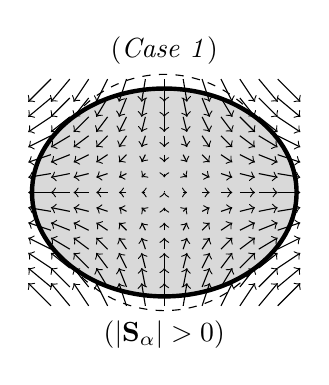
\begin{tikzpicture}[ultra thick,scale=0.6]
        \def\nRows{6}
        \def\nCols{6}
        \draw[dashed,thin] (0,0)circle(2.5);
        \draw[fill=gray!30] (0,0)ellipse(2.8 and 2.2);
        \foreach \x in {-\nRows,...,\nRows} {
            \foreach \y in {-\nCols,...,\nCols} {
                \pgfmathsetmacro\distance{veclen(\x*0.4, \y*0.4)};
                \pgfmathparse{\distance < 2.45 ? "blue" : "white"}
                \edef\colour{\pgfmathresult};
                \ifthenelse{\equal{\colour}{blue}}{                    
                    \draw[thin,->](\x*0.4,\y*0.4)--++(0.08*\x,-0.08*\y);
                }
            }
        }
        \node (txt) at (0,3){(\textit{Case 1})};
        \node (txt) at (0,-3){($|\textbf{S}_\alpha| > 0$)};
    \end{tikzpicture}
     \hfill
    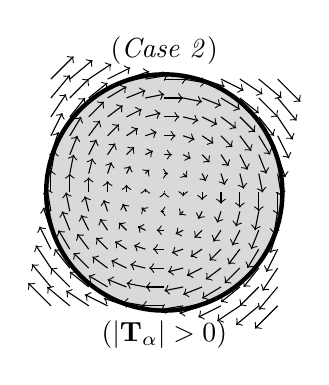
\begin{tikzpicture}[ultra thick,scale=0.6]
        \def\nRows{6}
        \def\nCols{6}
        \draw[fill=gray!30] (0,0)circle(2.5);
        \foreach \x in {-\nRows,...,\nRows} {
            \foreach \y in {-\nCols,...,\nCols} {
                \pgfmathsetmacro\distance{veclen(\x*0.4, \y*0.4)};
                \pgfmathparse{\distance < 2.5 ? "blue" : "white"}
                \edef\colour{\pgfmathresult};
                \ifthenelse{\equal{\colour}{blue}}{                    
                    \draw[thin,->](\x*0.4,\y*0.4)--++(0.08*\y,-0.08*\x);
                }
            }
        }
        \node (txt) at (0,3){(\textit{Case 2})};
        \node (txt) at (0,-3){($|\textbf{T}_\alpha| > 0$)};
    \end{tikzpicture}
    \hfill
    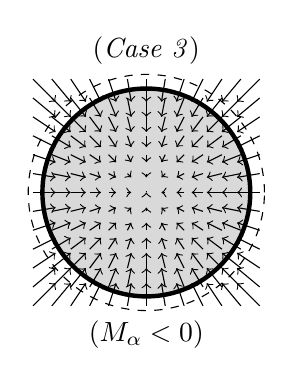
\begin{tikzpicture}[ultra thick,scale=0.6]
        \def\nRows{6}
        \def\nCols{6}
        \draw[dashed,thin] (0,0)circle(2.5);
        \draw[fill=gray!30] (0,0)circle(2.2);
        \foreach \x in {-\nRows,...,\nRows} {
            \foreach \y in {-\nCols,...,\nCols} {
                \pgfmathsetmacro\distance{veclen(\x*0.4, \y*0.4)};
                \pgfmathparse{\distance < 2.3 ? "blue" : "white"}
                \edef\colour{\pgfmathresult};
                \ifthenelse{\equal{\colour}{blue}}{                    
                    \draw[thin,->](\x*0.4,\y*0.4)--++(-0.08*\x,-0.08*\y);
                }
            }
        }
        \node (txt) at (0,3){(\textit{Case 3})};
        \node (txt) at (0,-3){($M_\alpha < 0$)};
    \end{tikzpicture}
    \hfill
    \caption{Graphical representation of the inner kinematics of an arbitrary particle under three scenarios. 
        The arrows represent the velocity field inside the particle, $\textbf{w}_d^0$, with the corresponding value of the moment of momentum tensor indicated below. 
        The operator $|\ldots|$ refers to the norm of the tensors. 
        According to the inner velocity field:
        (\textit{Case 1}) The particle experiences a mean rate of deformation, resulting in non-zero stretching of momentum along the principal axis of deformation;
        (\textit{Case 2}) The particle is rotating, leading to a non-zero angular momentum vector in the direction of rotation;
        (\textit{Case 3}) The particle undergoes compression, resulting in a negative trace of the moment of momentum.
    }
    \label{eq:scheme}
\end{figure}

% \subsection{Conservation laws}



% \subsubsection{Inside the volume}

 


% Let us consider the specific case of the momentum balance, i.e. $q_\alpha = \textbf{p}_\alpha$.
% In this situation, \ref{eq:dt_q_alpha} reads
% \begin{equation}
%     \ddt  \textbf{p}_\alpha
%     = \intO{ \rho_d\textbf{g} }
%     + \intS{ 
%         \left[
%         f_d^0 (\textbf{u}_I^0-\textbf{u}_d^0)
%          + \bm{\sigma}_d^0%\cdot\textbf{n}_d  
%         %+ \mathbf{\Phi}_d^0 
%         \right] 
%         \cdot \textbf{n}_d },
% \end{equation}
% first term reads as $\intO{ \rho_d\textbf{g} }$ 
% The first term on the right-hand side represents the total weight acting on the particle $\alpha$, 
% the second term represents the total source of momentum due to phase transfer, and it is expressed as, $\intS{ \rho_d \textbf{u}_d^0 (\textbf{u}_I^0-\textbf{u}_d^0)\cdot\textbf{n}_d }$,
% and the last term $\intS{ \bm{\sigma}_d^0\cdot\textbf{n}_d }$, represents the resultant of the hydrodynamic forces acting on the surface of the particle.
% It is important to notice that under this form, the exchange terms are expressed as integrals of dispersed phase fields denoted by the subscript $_d$.
% Nevertheless, depending on the nature of the dispersed phase, these fields may not always be defined.
% For rigid particles the stress within the particle $\bm{\sigma}_d^0$ is indeterminate \citep{guazzelli2011}.  
% Hence, our objective is to express these exchange terms, in terms of the continuous phase field quantities instead of the dispersed phase fields, i.e. in terms of $\mathbf{\Phi}_f^0$ and $\textbf{u}_f^0$ rather than $\mathbf{\Phi}_d^0$ and $\textbf{u}_d^0$. 

%\subsubsection{On the interfaces}
 

%For completeness, we exposed in \ref{ap:particles_eq} a clear derivation of the mass, momentum and total energy equations for a single particle.
%The derivation takes place using the same hypothesis as it is exposed in \ref{ap:hypothesis}.
%Especially, it is shown that the integration of the kinetic energy jump condition corresponds to the Lagrangian derivative of the particle surface, see \ref{eq:int_u_I2}.

%  \section{Lagrangian equation for a single particle}
\label{ap:particles_eq}
\tb{MAYBE EXPLICITE A BIT MORE THE BOUNDARY FOR ENERRGY}
Following the same assumption as in \ref{sec:local_eq}, i.e. we consider no mass transfer and weightless interfaces, the Lagrangian  mass, momentum and energy equations for a single particle can be derived using the generic form \ref{eq:dt_q_alpha_tot} and reads as, 
\begin{align}
    \label{eq:dt_m_alpha}
    \ddt m_\alpha
    &= 
    0\\
    \label{eq:dt_p_alpha}
    \ddt (m_\alpha \textbf{u}_\alpha)
    &= 
    m_\alpha\textbf{g}
    +  \intS{\bm{\sigma}_1^0 \cdot \textbf{n}_2}\\
    \label{eq:dt_E_alpha_tot}
    \ddt (m_\alpha E_\alpha^\text{tot})
    &= 
    m_\alpha \textbf{u}_\alpha \cdot \textbf{g}
    +\textbf{u}_\alpha \cdot \intS{\bm{\sigma}_1^0 \cdot \textbf{n}_2}
    +\intS{\textbf{w}_1^0 \cdot \bm{\sigma}_1^0 \cdot  \textbf{n}_2} 
    - \intS{\textbf{q}_1^0 \cdot \textbf{n}_2}
\end{align}
where  $\intS{  \bm{\sigma}_1^0 \cdot \textbf{n}_2 }$ is the resultants of the hydrodynamic force and $\intS{ \textbf{q}_1^0 \cdot \textbf{n}_2 }$ is the resultants of the surface heat flux. 
The second term on the right hands side of the energy equation is the work produced by the mean force and the translational motion of the droplets, while $\intS{\textbf{w}_1^0 \cdot \bm{\sigma}_1^0 \cdot  \textbf{n}_2}$ is the work produced by the local forces and local motion of the fluid at the surface of the particle.
Since we integrated the energy over the particle's volume and its surface, we explicitly made appear the surface energy $\gamma s_\alpha$ within the derivative operator. 
Note that these equations does not explicitly account for inter-particle interactions. 
However, it is possible to include manually such forces by noticing that the surface external stress flux $\bm{\sigma}_1^0$ is the sum of hydrodynamic and particles-particles interaction forces, regardless it is pure contact forces from direct contact or a force mediated through the carrier fluid.
From this consideration it is possible to split every term involving the stress $\bm{\sigma}_1^0$ into two terms representing these contributions. 
Same comments can be made for the heat flux $\textbf{q}_1^0$. 
Although this distinction is important, for purpose of clearly we will stay general, and we will keep the fluxes $\bm{\sigma}_1^0$ and $\textbf{q}_1^0$ as such. 

In the spirit of the energy decomposition exposed in \ref{eq:E_alpha_def} the total energy equation can be split into three equations, one for the center of mass kinetic energy, internal motion and internal kinetic energy, namely,  
\begin{align}
    \label{eq:dt_u2_alpha}
    \frac{1}{2}\ddt (m_\alpha u_\alpha^2)
    &= 
    \textbf{u}_\alpha\cdot
    \textbf{g}m_\alpha
    + 
    \textbf{u}_\alpha\cdot
    \intS{\bm\sigma_1^0 \cdot \textbf{n}_2},\\
    \label{eq:dt_w2_alpha}
    \ddt (W_\alpha + \gamma s_\alpha)
    &= 
    \intS {\textbf{w}_1^0 \cdot \bm{\sigma}_1^0 \cdot \textbf{n}_2 }
    - \intO{ \bm{\sigma}_2^0 : \grad\textbf{u}_2^0 }
    \\
     \label{eq:dt_e_alpha}
    \ddt (m_\alpha e_\alpha )
    &= 
     \intO{ \bm{\sigma}_2^0 : \grad\textbf{u}_2^0  }
    -  \intS{\textbf{q}_1^0\cdot \textbf{n}_2 } 
\end{align}
respectively. 
The first equation is obtained by taking the dot product of \ref{eq:dt_p_alpha} with $\textbf{u}_\alpha$. 
The third equation is directly obtained using the local conservation of $e_k^0$ (\ref{eq:dt_rhoe_k}) and setting $f_2^0 = e_2^0$ in \ref{eq:dt_q_alpha_tot}.
The last equation is then obtained by subtracting the first and third equations to \ref{eq:dt_E_alpha_tot}. 
Note that in \citet{eq:dt_w2_alpha} the use of \ref{eq:dt_rhoI_uI2} makes appear explicitly the derivative of the surface energy $s_\alpha \gamma$. 
Note that under this form we see that the energy loss in the deformation represented by $W_p$ will be gathered in the surface energy which will in turn act as a source term in the internal kinetic energy motion.
The surface tension plays the role as a spring in the energy balance.   
From this set of equation we can easily see that the rate of dissipation terms $\intS{\bm{\sigma}_2^0 : \grad\textbf{u}_2^0}$ represent an energy sink in the equation of $W_\alpha$ while it is a source term in the internal energy equation. 
As it has been observed in the previous section, this terms convert the energy of internal motion to molecular agitation. 
However, the interplay between the center of mass  kinetic energy and the internal fluctuation is not obvious and has no common term with the heat and internal kinetic energy equation.
In fact, we will see that the transfer between these scales is archived thought the fluid phase pseudo turbulent energy. 


% \section{Averaged two-fluid model}
\label{ap:two-fluid_model}
Before introducing the \textit{hybrid model} which will be the subject of the next section, we expose in the first place the classic averaged two-fluid model. 

\subsection{Averaged volume equations}
Using the generic formulation \ref{eq:avg_dt_chi_f} and the local expression of the mass, momentum and total energy equation, i.e. : \ref{eq:dt_rho}, \ref{eq:dt_rhou_k} and \ref{eq:dt_rhoE_k} we easily find the averaged form of the mass, momentum and total energy equation.
They read, 
\begin{align}
    \label{eq:dt_avg_rho_k}
    \pddt (\phi_k \rho_k)  
    + \div (
        \phi_k \rho_k\textbf{u}_k
    )
    &= 
    0,\\
    \label{eq:dt_avg_rhou_k}
    \pddt (\phi_k \rho_k\textbf{u}_k)  
    + \div (
        \phi_k \rho_k\textbf{u}_k\textbf{u}_k
        + \bm{\sigma}_k^\text{eq}
    )
    &= 
    \phi_k \rho_k \textbf{g} 
    +  \avg{\delta_I \bm{\sigma}_k^0 \cdot \textbf{n}_k},\\
    \label{eq:dt_avg_rhoE_k}
    \pddt (\phi_k\rho_kE_k)  
    + \div (
        \phi_k\rho_kE_k\textbf{u}_k
        + \bm{q}_k^\text{eq}
        + \textbf{u}_k \cdot \bm{\sigma}_k^\text{eq}
        % - \textbf{u}_k^0 \cdot \bm{\sigma}_k^0 
        % + \textbf{q}_k^0
        )
    &= 
    \phi_k \rho_k\textbf{u}_k \cdot \textbf{g} 
    + \avg{\delta_I (\textbf{u}_k^0 \cdot \bm{\sigma}_k^0 - \textbf{q}_k^0)\cdot \textbf{n}_k},
\end{align} 
respectively. 
Where we have introduced the effective stress and heat fluxes namely, 
\begin{align*}
    &\bm{\sigma}_k^\text{eq}
    = 
     \rho_k\avg{\chi_k \textbf{u}_k'\textbf{u}_k'}
      - \phi_k \bm{\sigma}_k,%- n_p \textbf{M}_p
    &\textbf{q}_k^\text{eq}
    =\textbf{q}_k^\text{e} +\textbf{q}_k^\text{k},  \\
    &\textbf{q}_k^\text{e}
    = \rho_k \avg{\chi_k\textbf{u}_k' e_k'} 
    + \phi_k\textbf{q}_k,
    &\textbf{q}_k^\text{k}
    = \rho_k \avg{\chi_k \textbf{u}_k' k_k} 
    - \avg{\chi_k \textbf{u}_k' \cdot \bm{\sigma}_k^0}.
\end{align*}
The main differences between these equations and their microscale counterpart, is that : 
(1) we have introduced a pre factor $\phi_k$ in front of most the unknown  ($\textbf{u}_k$ and $E_k$), 
(2) the non-convective fluxes appear under the form of an effective tensor containing the covariance of the quantity to be conserved with the local velocity of the phase, 
and (3) a new source term appear on the RHS accounting for the exchange across the phases. 
Additionally, it is interesting to notice that the effective fluxes of the total energy is written as the mean work done by the effective stress of the momentum $\textbf{u}_k \cdot \bm{\sigma}_k^\text{eq}$ plus an effective heat flux $\bm{q}_k^\text{eq}$. 

The terms $\avg{\chi_k \textbf{u}_k'\textbf{u}_k'}$ will be referred as the Reynolds stress or pseudo turbulent stress. 
It has a fundamental importance in the multiphase flow problem as it appear in \ref{eq:dt_avg_rhou_k} and as we see now its trace is related to the mean kinetic energy. 
Indeed, the phase averaged total energy can be further decompose into three energy components, that is,  
\begin{align}
    E_k = e_k + k_k + u_k^2/2
    \label{eq:E_def2}
\end{align}
where $k_k$ is the pseudo-turbulent kinetic energy defined as, $\phi_k k_k = \frac{1}{2}\avg{\chi_k \textbf{u}_k'\cdot \textbf{u}_k'}$. 
Each of the components of the total energy represent the averaged agitation at different scales. 
From molecular agitation which quantified by $e_k$, to the macroscopic scale agitation or kinematic energy $u_k^2$, and in between we find the pseudo turbulent energy $k_k$ which represents the local scale velocity fluctuation. 
To fully describe the averaged total energy one must add at least a supplementary equation either for $k_k$ or $e_k$ assuming \ref{eq:dt_avg_rhoE_k} is solved. 
Using \ref{eq:dt_avg_rhou_k} dotted with $\textbf{u}_k$ yields an equation for the mean kinetic energy. 
Averaging \ref{eq:dt_rhoe_k} yields un equation for $e_k$.  
Then, subtracting these two equations to \ref{eq:dt_avg_rhoE_k} gives us an equation for $k_p$. 
The kinetic energy, pseudo turbulent and internal averaged equations are, 
\begin{align}
    \label{eq:dt_avg_uk2}
    &\pddt (\phi_k \rho_ku_k^2/2)  
    + \div (
        \phi_k \rho_k\textbf{u}_ku_k^2/2
        + \textbf{u}_k \cdot \bm{\sigma}_k^\text{eq}
    )
    = 
    \bm{\sigma}_k^\text{eq} : \grad \textbf{u}_k
    + \phi_k \rho_k \textbf{u}_k\cdot \textbf{g} 
    +  \textbf{u}_k\cdot \avg{\delta_I \bm{\sigma}_k^0 \cdot \textbf{n}_k},\\
    \label{eq:dt_avg_kk}
    &\pddt (\phi_k\rho_kk_k)  
    + \div (
        \phi_k\rho_kk_k\textbf{u}_k
        + \textbf{q}_k^\text{k} 
        )
    = 
    - \avg{\chi_k\bm{\sigma}_k^0 : \grad \textbf{u}_k^0}
    - \bm{\sigma}_k^\text{eq} : \grad \textbf{u}_k
    + \avg{\delta_I \textbf{u}_k' \cdot \bm{\sigma}_k^0 \cdot \textbf{n}_k},\\
    \label{eq:dt_avg_ek}
    &\pddt (\phi_k\rho_ke_k)  
    + \div (
        \phi_k \rho_ke_k\textbf{u}_k
        +
        \textbf{q}_k^\text{e} 
        )
    = 
    \avg{\chi_k\bm{\sigma}_k^0 : \grad \textbf{u}_k^0}
    - \avg{\delta_I \textbf{q}_k^0 \cdot \textbf{n}_k},
\end{align}
respectively. 
This derivation is in agreement with \citet{morel2015mathematical}. 
Under this form the energy transfer across scale is clear. 
Indeed, the term $\bm{\sigma}_k^\text{eq} : \grad \textbf{u}_k$ act as a sink term in \ref{eq:dt_avg_uk2} and a source term in \ref{eq:dt_avg_kk}, while the averaged diffusive terms $\avg{\chi_k\bm{\sigma}_k^0 : \grad \textbf{u}_k^0}$ is a sink in \ref{eq:dt_avg_kk} and a source in \ref{eq:dt_avg_ek}. 
To determine the total energy only two of the four energy equations must be solved. 
In practice, it is useful to solve one equation for $k_k$ since it is useful for the Reynolds stress modeling since $\avg{\chi_k \textbf{u}_k^0 \textbf{u}_k^0}: \bm\delta = 2 k_k$, and another for $e_k$ since $u_k^2$ is already determined by the momentum equation. 

\subsection{Averaged surface equations}
The volume averaged equations must be completed by an averaged surface transport equation.  
For this purpose we multiply \ref{eq:surface_tension}, \ref{eq:dt_rhoIe_I} and \ref{eq:dt_rhoI_uI3} by $\delta_I$ and apply the average operator.
By considering the topological equations we obtain the  momentum, kinetic and internal energy averaged surface equations, namely
\begin{align}
    \label{eq:dt_avg_uI}
    \avg{\delta_I \Jump{\bm{\sigma}^0_k}}
    &= -\gamma \div \avg{\delta_I (\bm\delta - \textbf{nn})},\\
    \label{eq:dt_avg_gamma}
    \avg{\delta_I \Jump{\textbf{u}_k^0 \cdot \bm{\sigma}^0_k}}
    &= - \gamma \left[
        \pddt \phi_I
        +  \div \avg{\delta_I (\textbf{u}_{I}^0 \cdot \textbf{n})\textbf{n} },
    \right]\\
    \avg{\delta_I \Jump{\textbf{q}^0_k}}
    &= 0
\end{align}
respectively. 
The first equation represents the contribution of the surface tension stresses to the bulk momentum equation.
The second equation represents the amount of energy stored as surface deformation.
And the last equation witnesses of the continuity of heat flux through the interface. 

\subsection{Averaged single fluid formulation}
Lastly, by summing the above formulations we can also derive equations for the bulk quantities. 
Indeed, summing \ref{eq:dt_avg_rho_k}, \ref{eq:dt_avg_rhou_k} and \ref{eq:dt_avg_rhoE_k} for $k=f,d$ with the surface equations one obtain the bulk conservation equations, 
\begin{align}
    \label{eq:dt_avg_rho}
    \pddt \rho 
    + \div (
         \rho \textbf{u}_m
    )
    &= 
    0,\\
    \label{eq:dt_avg_rhou}
    \pddt ( \rho\textbf{u}_m)  
    + \div (
         \rho\textbf{u}_m\textbf{u}_m
        + \bm{\sigma}^\text{eq}_m
    )
    &= 
     \rho \textbf{g} \\
    \label{eq:dt_avg_rhoE}
    \pddt (\rho E_m)  
    + \div (
        \rho E_m \textbf{u}_m
        + \bm{q}^\text{eq}_m
        + \textbf{u}_m \cdot \bm{\sigma}^\text{eq}_m
        % - \textbf{u}_k^0 \cdot \bm{\sigma}_k^0 
        % + \textbf{q}_k^0
        )
    &= 
     \rho \textbf{u}_m  \cdot \textbf{g} 
\end{align} 
respectively. 
Where we have introduced the effective stress and heat fluxes namely, 
\begin{align*}
    &\bm{\sigma}^\text{eq}_m
    = 
    \avg{ \rho^0\textbf{u}'_m\textbf{u}'_m}
      - \phi_f\bm\sigma_f
      - \phi_d\bm\sigma_d
      - \phi_I\bm\sigma_I,%- n_p \textbf{M}_p
    &\textbf{q}^\text{eq}_m
    =\textbf{q}^\text{e}_m +\textbf{q}^\text{k}_m,  \\
    &\textbf{q}^\text{e}_m
    = \avg{\rho^0\textbf{u}_m' e_m'} 
    + \phi\textbf{q}_m,
    &\textbf{q}^\text{k}_m
    = \avg{\rho^0 \textbf{u}_m' k_m} 
    - \avg{ \textbf{u}_m' \cdot \bm{\sigma}^0}.
\end{align*}
In these equations we have make use of the subscript $_m$ to denote the Favre average quantities, such that, 
\begin{align*}
    \rho \textbf{u}_m
    = \avg{\rho^0 \textbf{u}^0}
    &&
    \rho E_m
    = \avg{\rho^0 \textbf{u}^0}
    &&
    \rho e_m
    = \avg{\rho^0 \textbf{u}^0}
\end{align*}
Likewise, the fluctuating quantity are written as, 
\begin{equation}
    \textbf{u}_m'
    = \textbf{u}^0 - \textbf{u}_m.
\end{equation}
In \ref{eq:dt_avg_rhoE} we have defined the bulk total energy as the average of the sum of the local energy, namely, 
\begin{equation}
    \rho E_m = \avg{\sum_k \rho_k [e_k^0 + \frac{1}{2}(u_k)^2] 
    + \delta_I \gamma}
    = \rho( e_m +  k_m + \frac{1}{2}u_m^2)
\end{equation}
with, $e_m = \avg{\sum_k \rho_k\phi_k e_k + \phi_I \gamma}$ and $k = \avg{\rho^0 \textbf{u}'\cdot \textbf{u}'}/2$. 


These equations are particularly interesting from an experimental point of view. 
% Indeed, as in experiment we cannot distinguish between the details of both phase. 
For example in a Rheometer we are able to measure only for the \textit{Bulk stress} $\bm\sigma^\text{eq}_m$ and not $\bm\sigma^\text{eq}_f$ and $\bm\sigma^\text{eq}_d$ separately, as it measure the stress response from the mixture phases. 
Therefore, it is of interest to describe a bit more in details the \textit{Bulk stress}, which is the subject of the next section.
% 

\subsection{The bulk stress in dispersed multiphase flow}


Now that the architecture of the averaged dispersed multiphase flow equation is clarified, we would like to present the expression of the bulk stress tensor in a suspension of inertial particles subject to an arbitrary local body force field, $\textbf{b}^0$.
Firstly, is important to recall the definition of the \textit{bulk stress}. 
We define the \textit{bulk stress} tensor as a force applied on the fluid and on the particles phase, having the form $\div \bm{\Sigma}$, which added to the total external force $\textbf{B}$, balance exactly the material derivative of the mixture momentum : $\frac{D \rho \textbf{u}}{Dt}$. 
In this definition $\textbf{B}$ cannot be decomposed into a vector and a divergence of a tensor, in which case the latter would just contribute to $\bm{\Sigma}$.
Equally, we insist on the fact that the momentum considered is $\rho\textbf{u}$ which is the bulk momentum. 

We first expose the averaged mixture momentum and angular momentum equation easily derived from \ref{eq:dt_avg_f}, 
\begin{align}
    \pddt (\rho u_i)
    + \partial (\rho u_iu_k
    + \sigma_{ik}^\text{eq})
    = b_i\\
    \epsilon_{ijk} \sigma_{jk}
    = 0 
    \label{eq:momentum_bulk}
\end{align}
In the momentum equation we have defined, $\sigma_{ik}^\text{eq} = \avg{\rho\textbf{u}'\textbf{u}'}
- \avg{\chi_1\bm{\sigma}_1^0}-\avg{\chi_2\bm{\sigma}_2^0} - \avg{\delta_I \bm{\sigma}_I^0}$. 
Additionally, in the averaged angular momentum equation we have assumed that no-body torque exist at the local scale making the second equality equal to $0$ \citet{leal2007advanced} and the averaged mixture stress $\bm{\sigma}$ a symmetric quantity. 
However, note that $\bm{\sigma}$ is not exactly equal to the \textit{bulk stress} tensor $\bm{\Sigma}$ since $\textbf{b}$ can be expressed as a divergence of a stress.
Indeed, have defined $\textbf{b} = \textbf{B} + \div  \pMOavg{\textbf{b}_2^0}$ where $\textbf{B} = \phi_1 \textbf{b}_1 +  \pOavg{\textbf{b}_2^0 }$ and  $\pMOavg{\textbf{r}\textbf{b}_2^0}$ is defined accordingly to the previous definition. 
It follows the definition of the \textit{bulk stress} : 
\begin{equation}
    \bm{\Sigma}
    = 
    \avg{\rho\textbf{u}'\textbf{u}'}
    - \avg{\chi_1\bm{\sigma}_1^0}
    - \avg{\chi_2\bm{\sigma}_2^0} 
    - \avg{\delta_I \bm{\sigma}_I^0}
    - \pMOavg{\textbf{r}\textbf{b}_2^0}
\end{equation}
which proves already, in the absence of particles moments of the body forces $\pMOavg{\textbf{r}\textbf{b}_2^0}$, the antisymmetric part of the suspension stress is null, in agreement with \citet{dolata2020heterogeneous}.
% This skew symmetric part can be written in vector form as, 
% \begin{equation*}
%     \epsilon_{ijk}\textbf{T}_{jk}
%     = 
%     -\epsilon_{ijk} \pOavg{r_kb_j}
%     -\epsilon_{ijk}\frac{1}{2}\partial_l \pOavg{r_lr_kb_j}
%     = 0  
% \end{equation*}
We recall that the carrier fluid is a Newtonian fluid, therefore we may express the fluid phase stress as, 
\begin{equation}
    \phi_1 \sigma_{1,jk}
    = -p_1 \delta_{jk}
    + \mu_1 e_{jk}
    - \mu_1 \phi_2 e_{2,jk}. 
\end{equation} 
Additionally, we use the methodology of \citep{lhuillier1992volume,lhuillier1996contribution} to re express the averaged particle stress terms. 
The divergence of the particle phase stress may be expressed using \ref{eq:f_exp}, 
\begin{align}
    \label{eq:exp_sigma22}
    \partial_k \avg{\chi_2 {\sigma}_2^0}_{ik}
    &=  \partial_k\pOavg{ {\sigma}_{2,ik}^0}
    -\frac{1}{2} \partial_k\partial_j
    \pOavg{ r_j{\sigma}^0_{2,ik} + r_k\sigma^0_{2,ij}}
    + \ldots  \\
    \label{eq:exp_sigmaI2}
    \partial_k \avg{\delta_I {\sigma}^0_I}_{ik} 
    &=  \partial_k\pSavg{ {\sigma}_{I,ik}^0 }
        -\frac{1}{2} \partial_k\partial_j \pSavg{ r_j {\sigma}_{I,ik}^0+r_k {\sigma}_{I,ij}^0 }
        + \ldots  
\end{align}
Note that the heterogeneous terms must remain symmetric in the index $kj$ due to the double contraction with the operator $\partial_k\partial_j$, thus only the symmetric part in $jk$ remain and the terms such as, $\pOavg{ r_j{\sigma}^0_{2,ik} - r_k\sigma^0_{2,ij}}$ vanish. 
Upon the use of the moment of momentum equation of the first and second order we can easily derive these expressions, 
\begin{align}
    \intS{ (\bm{\sigma}_I)_{ik}}
    +\intO{ (\bm{\sigma}_2^0)_{ik}}
    = 
    \intO{ \rho_2 
    (\textbf{w}_2^0\textbf{w}_2^0  )_{ik}
    }
    -\ddt \intO{ r_i (\textbf{u}^0_2)_k }
    +\intS{ 
        b_{i}
        r_k 
    }
    +\intS{ 
     r_i (\bm{\sigma}_1^0 \cdot \textbf{n}_2)_{k}
    }\\
    \intO{ r_{j}(\bm{\sigma}^0_2)_{ik}+r_{k}(\bm{\sigma}^0_2)_{ji}}
    +\intS{ r_{j}(\bm{\sigma}^0_I)_{ik}+r_{k}(\bm{\sigma}_I^0)_{ji}}
    = 
    - \ddt\intO{ \rho_2 (\textbf{u}_2^0)_i r_j r_k }\nonumber\\
    + \intO{ \rho_2 (r_{j} (\textbf{w}_2^0)_k (\textbf{u}^0_2)_i + r_k (\textbf{w}_2^0)_j (\textbf{u}^0_2)_i)}
    +\intS{  r_{k}r_{j} (\bm{\sigma}_1^0)_{il} (\textbf{n}_2)_l }
    + \intO{ r_{k}r_{j}  \rho_2 b_i } 
    \label{eq:dt_P2_alpha}
\end{align}
It is evident that by using an arbitrary order of moment of momentum equation one can substitute any volume integral of the particle stress appearing in the expansion \ref{eq:exp_sigma22}. 
% By consideration of symmetric of the local stress, it is evident that the skew symmetric part of the moment of momentum will not have any dynamical role thus we can retrieve the average of \ref{eq:dt_mu_alpha} to the first relation. 
% To extract the skew symmetric part we start by writing the permutation of these equations with $ik$ yielding,  
% \begin{align}
%     \intS{ 
%     (\bm{\sigma}_I)_{ki}
%     }
%     +\intO{ 
%     (\bm{\sigma}_2^0)_{ki}
%     }
%     = 
%     \intO{ \rho_2 
%     (\textbf{w}_2^0\textbf{w}_2^0  )_{ki}
%     }
%     -\ddt \intO{ r_k (\textbf{u}^0_2)_i }
%     +\intS{ b_{k}r_i }
%     +\intS{ r_k (\bm{\sigma}_1^0 \cdot \textbf{n}_2)_{i}}\\
%     \intO{ r_{j}(\bm{\sigma}^0_2)_{ki}+r_{i}(\bm{\sigma}^0_2)_{jk}}
%     +\intS{ r_{j}(\bm{\sigma}^0_I)_{ki}+r_{i}(\bm{\sigma}_I^0)_{jk}}
%     = 
%     - \ddt\intO{ \rho_2 (\textbf{u}_2^0)_k r_j r_i }\nonumber\\
%     + \intO{ \rho_2 (r_{j} (\textbf{w}_2^0)_i (\textbf{u}^0_2)_k + r_i (\textbf{w}_2^0)_j (\textbf{u}^0_2)_k)}
%     +\intS{  r_{i}r_{j} (\bm{\sigma}_1^0)_{kl} (\textbf{n}_2)_l }
%     + \intO{ r_{i}r_{j}  \rho_2 b_k } \\
%     \intO{ r_{i}(\bm{\sigma}^0_2)_{jk}+r_{k}(\bm{\sigma}^0_2)_{ij}}
%     +\intS{ r_{i}(\bm{\sigma}^0_I)_{jk}+r_{k}(\bm{\sigma}_I^0)_{ij}}
%     = 
%     - \ddt\intO{ \rho_2 (\textbf{u}_2^0)_j r_i r_k }\nonumber\\
%     + \intO{ \rho_2 (r_{i} (\textbf{w}_2^0)_k (\textbf{u}^0_2)_j 
%     + r_k (\textbf{w}_2^0)_i (\textbf{u}^0_2)_j)}
%     +\intS{  r_{k}r_{i} (\bm{\sigma}_1^0)_{jl} (\textbf{n}_2)_l }
%     + \intO{ r_{k}r_{i}  \rho_2 b_j } 
% \end{align}
% Acknowledgement of the symmetrical nature of $\bm{\sigma}_2^0$ and $\bm{\sigma}_I^0$ gives the following antisymmetrical balance equations, 
% \begin{align}
%     0
%     = 
%     -\ddt \intO{ r_i (\textbf{u}^0_2)_k -r_k (\textbf{u}^0_2)_i }
%     +\intS{ b_{i}r_k -b_{k}r_i }
%     +\intS{r_i (\bm{\sigma}_1^0 \cdot \textbf{n}_2)_{k} - r_k (\bm{\sigma}_1^0 \cdot \textbf{n}_2)_{i}}\\
%     \intO{ r_{j}(\bm{\sigma}^0_2)_{ik}
%             -r_{i}(\bm{\sigma}^0_2)_{jk}}
%     +\intS{ r_{j}(\bm{\sigma}^0_I)_{ik}
%            - r_{i}(\bm{\sigma}_I^0)_{jk}}
%     = 
%     - \ddt\intO{ \rho_2 (\textbf{u}_2^0)_i r_j r_k -  \rho_2 (\textbf{u}_2^0)_j r_i r_k }\nonumber\\
%     + \intO{ \rho_2 (r_{j} (\textbf{w}_2^0)_k (\textbf{u}^0_2)_i + r_k (\textbf{w}_2^0)_j (\textbf{u}^0_2)_i)}
%     - \intO{ \rho_2 (r_{i} (\textbf{w}_2^0)_k (\textbf{u}^0_2)_j + r_k (\textbf{w}_2^0)_i (\textbf{u}^0_2)_j)}\\
%     +\intS{  r_{k}r_{j} (\bm{\sigma}_1^0)_{il} (\textbf{n}_2)_l 
%     -r_{k}r_{i} (\bm{\sigma}_1^0)_{jl} (\textbf{n}_2)_l }
%     + \intO{ r_{k}r_{j}  \rho_2 b_i
%     - r_{k}r_{i}  \rho_2 b_j } 
% \end{align}
% The last equation need to be added to the second permutation which gives, 
% \begin{align*}
% \intO{ r_{j}(\bm{\sigma}^0_2)_{ik}}
% +\intS{ r_{j}(\bm{\sigma}^0_I)_{ik}}
% = 
% - \ddt\intO{ \rho_2 (\textbf{u}_2^0)_k r_j r_i 
% + \rho_2 (\textbf{u}_2^0)_i r_j r_k 
% -  \rho_2 (\textbf{u}_2^0)_j r_i r_k }\nonumber\\
% + \intO{ \rho_2 (r_{j} (\textbf{w}_2^0)_k (\textbf{u}^0_2)_i + r_k (\textbf{w}_2^0)_j (\textbf{u}^0_2)_i)}
% - \intO{ \rho_2 (r_{i} (\textbf{w}_2^0)_k (\textbf{u}^0_2)_j + r_k (\textbf{w}_2^0)_i (\textbf{u}^0_2)_j)}\\
% - \intO{ \rho_2 (r_{j} (\textbf{w}_2^0)_i (\textbf{u}^0_2)_k + r_i (\textbf{w}_2^0)_j (\textbf{u}^0_2)_k)}\\
% +\intS{  r_{k}r_{j} (\bm{\sigma}_1^0)_{il} (\textbf{n}_2)_l 
% +r_{j}r_{i} (\bm{\sigma}_1^0)_{kl} (\textbf{n}_2)_l 
% -r_{k}r_{i} (\bm{\sigma}_1^0)_{jl} (\textbf{n}_2)_l }
% + \intO{ r_{k}r_{j}  \rho_2 b_i
% + r_{j}r_{i}  \rho_2 b_k 
% - r_{k}r_{i}  \rho_2 b_j 
% } 
% \end{align*}
In, addition one must notice that the particle angular momentum balance equation doesn't involve the integral of the particle local stress and has therefore, no dynamical role in the equivalent stress expression. 
Making use of these remarks we obtain this general formula for the suspension stress,  
\begin{multline}
    \bm{\Sigma}
    = \avg{\rho\textbf{u}'\textbf{u}'}_{ik}
    + \phi_1 p_1 \delta_{ik}
    - \mu_1 e_{ik}
    % + \mu_1 \phi_2 e_{2,ik}. 
    - \pOavg{ \rho_2 (\textbf{w}_2^0\textbf{w}_2^0  )_{ik}}
    + \pavg{\ddt {\mathcal{S}_{ik}} }\\
    - \pSavg{ b_{i}r_k - b_{k}r_i }
    - \pSavg{ r_i (\bm{\sigma}_1^0 \cdot \textbf{n}_2)_{k}
    + r_k (\bm{\sigma}_1^0 \cdot \textbf{n}_2)_{i}}
    + \mu_1 \pOavg{e_2^0}_{ik}
    + \frac{1}{2} \div\bm{\Sigma}_1
    \label{eq:eq_stress}
\end{multline}
with the inhomogeneous stress gathered in $\bm{\Sigma}_1$, namely,
\begin{multline}
    \bm{\Sigma}_1
    = 
    - \pavg{\ddt\intO{ \rho_2 (\textbf{u}_2^0)_i r_j r_k }}
    + \pOavg{ \rho_2 (r_{j} (\textbf{w}_2^0)_k (\textbf{u}^0_2)_i + r_k (\textbf{w}_2^0)_j (\textbf{u}^0_2)_i)}\nonumber\\
    +\pSavg{  r_{k}r_{j} (\bm{\sigma}_1^0)_{il} (\textbf{n}_2)_l }
    - \mu_1 2 \pOavg{\textbf{r} \textbf{e}_2^0}_{jik}
\end{multline}
According to \ref{eq:scheme_equivalence}, expanding each component related to the dispersed phase in \ref{eq:momentum_bulk} one would see appear each moment of momentum equations under the divergence operator.
However, to stay consistent with the definition of the bulk stress tensor $\bm{\Sigma}$, we must keep the advecting term on the LHS of \ref{eq:momentum_bulk} unchanged, this is however not the case of the averaged body force term $\textbf{b}$ which allowed us to cancel all the body forces terms with the expansion of $\textbf{T}$.  

One of the major question in suspension dynamic raised by several authors, is the evaluation of the bulk stress or equivalent stress tensor of a suspension, see \citep{prosperetti2006stress, batchelor1970stress,zhang1997momentum,nadim1996concise} and more recently \citet{dolata2020heterogeneous}. 
The answer to this question is given in the general case of the generic averaged mixture equation. 
In light of \ref{eq:eq_stress} we have demonstrated how to express in a routine manner the bulk stress of the particle phase. 
And doing so without making appear explicitly the particles  internal stress. 
This, conclusion deserve several comments regarding previous studies. 
In  \citet{jackson1997locally},  the volume averaged momentum balance (equation (38) of \citet{jackson1997locally}) they make appear the higher moment of velocity of the particles as closure terms, these are hidden in $\pOavg{\textbf{w}_2^0 \textbf{w}_2^0}$.
However, in \citet{jackson1997locally} they did not remove the angular momentum to the stress yieldings a slightly different term. 
What we have shown here is that these higher moments of the particles phase such has the particles rotations have no dynamical significance in the mixture equations. 
Therefore, equation (38) of \citet{jackson1997locally} can be further simplified to the fluid and first order particle averaged equations. 
Equally, in the momentum mixture equation derived by \citet{zhang1997momentum} (equation (8.2)), they make appear explicitly the higher moment of acceleration and the higher moments of velocity in their equivalent stress. 
These terms must therefore simplify. 
In fact as, it could be supposed in their appendix these moments equally cancel. 
In agreement with \citet{dolata2021faxen} which also found that the only remaining part of the stress were solely the fluid phase exchange terms upon the calculation of the body forces moments. 
Similar, comments can be made on the study of \citet{prosperetti2006stress}. 
This also explain why \citet{nadim1996concise} found out that the interfacial terms of the surface tension and viscous interfacial forces play no direct role in the equivalent stress of the emulsion.

% \section{Application}
% \label{sec:application}
% \section{Averaged equations}



Now that we reached a clear understanding of the mathematical structures of the averaged two-phase flow equations we now expose the averaged set of equations which constitute the \textit{Hybrid model}. 
In this section we consider the simplifying assumption exposed in \ref{ap:hypothesis}. 
As mentioned in \ref{sec:two-fluid} we derive the mass, momentum and energy for the particles and continuous phase. 
Additionally, to describe the particle shape and inner velocity, one must consider the second moment of mass and first moment of momentum averaged equations. 
This, makes a total of 10 equations, 6 for the particle phase and 4 for the continuous phase.

To support the subsequent discussion, we provide the expressions of the closure terms of a dilute emulsion of spherical droplets. 
We will consider a monodisperse suspension of droplets with radius $a$ and constant viscosity $\lambda \mu_f$. 
% Additionally, both phases are assumed Newtonian therefore, $\bm{\sigma}_k^0 = - p_k^0 \bm\delta + \mu_k \textbf{e}_k^0$, with $\textbf{e}_k^0 = \grad \textbf{u}_k^0+(\grad \textbf{u}_k^0)^\dagger$ the shear rate tensor, $\bm\delta$ the identity tensor and $p_k ^0$ the local pressure. 
It must be understood that our goal is not to derive a set of equations for non-inertial spherical particles, in which case the energy equations and first order moment equations would be unnecessary. 
Instead, we provide the closures in stokes flow regime to illustrate their physical implication. 
Thus, even though the closures are expressed in the Stokes limit, note that the set of equations provided remains valid regardless of the flow regime.


\subsection{Averaged equations}

In this section we derive and discuss the averaged equations governing the continuous and teh dispersed  phase. 

\subsubsection{Continuous phases}


The equations for the carrier fluid are basically the same as in the classic two-fluid model derived in \ref{ap:two-fluid_model}, except that the interfacial terms of the form $\avg{\delta_I \ldots }$ need to be reformulated.
Indeed, the interfacial terms must be reformulated in terms of particle-averaged quantities in order to be consistent with the particle-phase equations \citep{jackson1997locally,zhang1994averaged}. 
This is achieved through the use of \ref{eq:f_exp} which enables us to convert the exchange terms appearing in \ref{eq:avg_dt_chi_f} into a series expansion of particle phase quantities. 
For clarity, we only retain the first, second and sometime third order terms of this expansion. 
The continuous phase averaged mass, momentum and total energy equations yield, 
\begin{align}
    \label{eq:dt_hybrid_rho}
    &\pddt (\phi_f \rho_f)  
    + \div (
        \phi_f \rho_f\textbf{u}_f
    )
    = 
    0,\\
    \label{eq:dt_hybrid_rhou_f}
    &\pddt (\phi_f \rho_f\textbf{u}_f)  
    + \div (
        \phi_f \rho_f\textbf{u}_f\textbf{u}_f
        + \bm{\sigma}_f^\text{eq}
    )
    = 
    \phi_f \rho_f \textbf{g} 
    - \pSavg{{\bm{\sigma}_f^0 \cdot \textbf{n}_d}},
    % +\div  \pSavg{{\textbf{r}\bm{\sigma}_f^0 \cdot \textbf{n}_d}}
    \\
    \label{eq:dt_hybrid_rhoE_f}
    &\pddt (\phi_f\rho_fE_f)  
    + \div (
        \phi_f\rho_fE_f\textbf{u}_f
        + \bm{q}_f^\text{eq}
        + \textbf{u}_f \cdot \bm{\sigma}_f^\text{eq}
        % - \textbf{u}_f^0 \cdot \bm{\sigma}_f^0 
        % + \textbf{q}_f^0
        )
    = 
    \phi_f \rho_f\textbf{u}_f \cdot \textbf{g} 
    - \textbf{u}_p \cdot \pSavg{{\bm{\sigma}_f^0 \cdot \textbf{n}_d}}\nonumber \\
    &- \pavg{ \textbf{u}_\alpha' \cdot \intS{  \bm{\sigma}_f^0 \cdot \textbf{n}_d}}
    - \pavg{ \intS{\textbf{w}_d^0 \cdot \bm{\sigma}_f^0 \cdot \textbf{n}_d}}
    + \pSavg{{\textbf{q}_f\cdot \textbf{n}_d}},
    % &\div [    
        % \textbf{u}_p \cdot \pSavg{{ \textbf{r}\bm{\sigma}_f^0 \cdot \textbf{n}_d}}
    % + \pavg{ \textbf{u}_\alpha' \cdot \intS{ \textbf{r} \bm{\sigma}_f^0 \cdot \textbf{n}_d}}
    % + \pavg{ \intS{\textbf{r}\textbf{w}_d^0 \cdot \bm{\sigma}_f^0 \cdot \textbf{n}_d}}
    % - \pavg{ \intS{\textbf{r}  \textbf{q}_f^0 \cdot \textbf{n}_d}}
    % ]
\end{align} 
respectively. 
Where we have introduced the equivalent stress tensor $\bm{\sigma}_f^\text{eq}$ and equivalent energy flux $\textbf{q}^\text{eq}_f$ as,
\begin{align}
    \label{eq:sigma_eq_def}
    \bm{\sigma}_f^\text{eq}
    =& 
    \avg{\chi_f\rho_f\textbf{u}_f'\textbf{u}_f'}
    - \phi_f \bm{\sigma}_f%- n_p \textbf{M}_p
    - \pSavg{{\textbf{r}\bm{\sigma}_f^0 \cdot \textbf{n}_d}}
    +\frac{1}{2}\div \pSavg{{\textbf{rr}\bm{\sigma}_f^0 \cdot \textbf{n}_d}}
    + \ldots
    \\
    \textbf{q}_f^\text{eq}
    =&\textbf{q}_f^\text{e} +\textbf{q}_f^\text{k} \nonumber \\
    \textbf{q}_f^\text{e}
    =& \rho_f \avg{\chi_f \textbf{u}_f' e_f'} 
    + \phi_f\textbf{q}_f 
    +\pSavg{{\textbf{r}\textbf{q}_f^0 \cdot \textbf{n}_d}} 
    -\frac{1}{2}\div \pSavg{{\textbf{rr}\textbf{q}_f^0 \cdot \textbf{n}_d}} 
    + \ldots
    \\
    \textbf{q}_f^\text{k}
    =& \rho_f \avg{\chi_f \textbf{u}_f' k_f} 
    - \avg{\chi_f \textbf{u}_f' \cdot \bm{\sigma}_f^0}
    + (\textbf{u}_f - \textbf{u}_p)\cdot
    \pSavg{{\textbf{r}\bm{\sigma}_f^0 \cdot \textbf{n}_d}}
    \label{eq:q_f_k_def}
    \\\nonumber &
    - \pavg{ \textbf{u}_\alpha' \cdot \intS{ \textbf{r} \bm{\sigma}_f^0 \cdot \textbf{n}_d}}
    - \pavg{ \intS{\textbf{r}\textbf{w}_d^0 \cdot \bm{\sigma}_f^0 \cdot \textbf{n}_d}}
    + \div[\ldots]
\end{align}
It is clear that those equations yield essentially the same as the previous set of equations presented in \ref{ap:two-fluid_model}.
The only difference is the presence of additional terms inside $\bm{\sigma}^\text{eq}_f$ and $\textbf{q}^\text{eq}_f$ due to the expansion of the interfacial terms. 
The $[\ldots]$ in \ref{eq:sigma_eq_def} to \ref{eq:q_f_k_def} refers to the higher moments of the expansion of the interfacial terms that are not display here for purpose of clarity. 
The averaged continuous-phase momentum balance \eqref{eq:dt_hybrid_rhou_f} under its \textit{hybrid} form was established long ago by \citet{zhang1997momentum,jackson1997locally}.  
\ref{eq:dt_hybrid_rhou_f} is of course consistent with the formulation given by these authors.

Now, let us discuss the continuous-phase averaged total energy balance \eqref{eq:dt_hybrid_rhoE_f}. 
Most of the terms have already been addressed in \ref{ap:two-fluid_model}, so for now, let's direct our attention to the exchange terms that have been re-formulated in this \textit{hybrid model}. 
% On the right-hand side of \ref{eq:dt_hybrid_rhoE_f} we identify four exchange terms.
Indeed, after taking the Taylor expansion of the interfacial term $\avg{\delta_I (\textbf{u}^0_d \cdot \bm{\sigma}_f^0 \cdot \textbf{n}_d)}$ on the right-hand side of \ref{eq:dt_avg_rhoE_k}, we used the following decomposition on each of the moments:
\begin{align}
    \label{eq:exergysource}
    \pavg{ \intS{\textbf{u}^0_d \cdot \bm{\sigma}_f^0 \cdot \textbf{n}_d}}
    &= 
    \textbf{u}_p \cdot \pSavg{{\bm{\sigma}_f^0 \cdot \textbf{n}_d}}
    + \pavg{ \textbf{u}_\alpha' \cdot \intS{  \bm{\sigma}_f^0 \cdot \textbf{n}_d}}
    + \pavg{ \intS{\textbf{w}_d^0 \cdot \bm{\sigma}_f^0 \cdot \textbf{n}_d}},
%     \label{eq:exergysource2}
%     \pavg{ \intS{\textbf{r}\textbf{u}^0_d \cdot \bm{\sigma}_f^0 \cdot \textbf{n}_d}}
%    &= 
%     \textbf{u}_p \cdot \pSavg{{\bm{\sigma}_f^0 \cdot \textbf{n}_d}}
%     + \pavg{ \textbf{u}_\alpha' \cdot \intS{\textbf{r}  \bm{\sigma}_f^0 \cdot \textbf{n}_d}}
%     + \pavg{ \intS{\textbf{r}\textbf{w}_d^0 \cdot \bm{\sigma}_f^0 \cdot \textbf{n}_d}},
\end{align}
where we have noticed that $\textbf{u}_d^0 = \textbf{u}_p + \textbf{u}_\alpha' +\textbf{w}_d^0$ according to \ref{eq:def_fluc_p} and to the definition of the particles \textit{inner velocity} $\textbf{w}_d^0$. 
Under this form the contribution of the kinetic energy exchange is explicit. 
Indeed, the first term on the right hands side of \ref{eq:exergysource} represents the work done by the mean particle-phase motion with the mean drag force.
The second term is the covariance term of the velocity of the particles with their respective drag forces.
Note that in a dilute suspension the drag force applied on each particle is likely to be a function of its instantaneous velocity, such as in \ref{eq:first_mom}, thus in a general manner this term is non-negligible. 
The last term represents the work made by the local force traction on the particle surface with the velocity at the surface of the particles $\textbf{w}_d^0$.
Regarding the higher order moment of kinetic energy exchange same comments can be made except that these terms act as energy fluxes instead of sources. 
The relative importance of these three contribution depends highly on the particles' nature. 
To our knowledge, such a decomposition is not present in the literature except in \citep[Chapter 2]{scorsim2021particle} where they make similar consideration, but for solid spherical particles.
We recall that the stress integral $\pSavg{\bm{\sigma}_f^0 \cdot \textbf{n}_d}$ could include particles-particles close interaction as well, making our model consistent with the latter study.

As mentioned in \ref{ap:two-fluid_model}, to fully describe the averaged total energy of the continuous phase one must add at least a supplementary equation, either for $k_k$ or $e_k$.  
Under the hybrid formulation, the kinetic energy, pseudo turbulent energy and internal energy equations read as,
\begin{align}
    \pddt (\phi_f \rho_fu_f^2/2)  
    + \div (
        \phi_f \rho_f\textbf{u}_fu_f^2/2
        + \textbf{u}_f \cdot \bm{\sigma}_f^\text{eq}
    )
    = 
    \phi_f \rho_f \textbf{u}_f\cdot \textbf{g} 
    + \bm{\sigma}_f^\text{eq} : \grad \textbf{u}_f
    -  \textbf{u}_f\cdot 
        \pSavg{{\bm{\sigma}_f^0 \cdot \textbf{n}_d}},
        \label{eq:dt_hybrid_u12}
        \\
    \label{eq:dt_hybrid_k1}
    \pddt (\phi_f\rho_fk_f)  
    + \div (
        \phi_f\rho_fk_f\textbf{u}_f
        + \textbf{q}_f^\text{k} 
        )
    = 
    - \avg{\chi_f\bm{\sigma}_f^0 : \grad \textbf{u}_f^0}
    - \bm{\sigma}_f^\text{eq} : \grad \textbf{u}_f\nonumber
    - \pavg{ \textbf{u}_\alpha' \cdot \intS{  \bm{\sigma}_f^0 \cdot \textbf{n}_d}}\\
    + (\textbf{u}_f - \textbf{u}_p)\cdot \pSavg{{\bm{\sigma}_f^0 \cdot \textbf{n}_d}} 
    - \pavg{ \intS{\textbf{w}_d^0 \cdot \bm{\sigma}_f^0 \cdot \textbf{n}_d}},
    \\
    \label{eq:dt_hybrid_e1}
    \pddt (\phi_f\rho_fe_f)  
    + \div (
        \phi_f \rho_fe_f\textbf{u}_f
        +
        \textbf{q}_f^\text{e} 
        )
    = 
    \avg{\chi_f\bm{\sigma}_f^0 : \grad \textbf{u}_f^0}
    + \pSavg{{\textbf{q}_f^0 \cdot \textbf{n}_d}},
\end{align}
respectively. 
One can verify that summing these three equations gives back \ref{eq:dt_hybrid_rhoE_f}. 
As \ref{eq:dt_hybrid_u12} and \ref{eq:dt_hybrid_e1} are rather similar to \ref{eq:dt_avg_uk2} and \ref{eq:dt_avg_ek} let us discuss \ref{eq:dt_hybrid_k1}. 
According to  \ref{eq:dt_hybrid_k1} we can stipulate that the pseudo turbulent energy $k_f$ in a dispersed two phase flow is generated by five different sources. 
The one corresponds to the local scale energy dissipation that acts as a source term in the internal equation \eqref{eq:dt_hybrid_e1} (first term on the right-hand of \ref{eq:dt_hybrid_k1}). 
The second contribution corresponds to the macroscopic dissipation term which is in fact the gradient of the mean fluid phase velocity contracted with the effective stress of the momentum equation.  
The last three exchange terms correspond to the generation of energy made by the particles through three distinct mechanism, which are given by \ref{eq:exergysource}. 
Note that \eqref{eq:dt_hybrid_k1} is consistent with those in former studies \citep[Chapter 7]{morel2015mathematical}\citep[Chapter 2]{scorsim2021particle}\citet{kataoka1989basic}. 
However, the decomposition of the exchange term is not present \eqref{eq:exergysource}, and the expression of $\textbf{q}_f^k$ with the first moment of the exchange term has not been exposed in the literature in such generality.
Additionally, it seems that the identification of the effective stress $\bm\sigma^\text{eq}_f$ in the energy equations have not been remarked up to now.
At least in the \textit{hybrid formulation} of the energy equations. 
The energy exchange between the macroscopic, microscopic, internal energy as well as the energy exchange between both phases, will be addressed later on.   


\subsubsection{Dispersed phase}

Now, we turn our attention to the particle phase equations and closure terms. 
By applying the ensemble average on the particle phase equations, namely \ref{eq:dt_m_alpha}, \ref{eq:dt_p_alpha} and \ref{eq:dt_E_alpha_tot} we obtain the particle-phase averaged mass, momentum and energy equations, namely, 
\begin{align}
    \label{eq:dt_hybrid_mp}
    \pddt \left(n_p m_p\right)
    + \div \left(n_pm_p\textbf{u}_p
    \right)
    = 
    0\\
    \label{eq:dt_hybrid_up}
    \pddt \left(n_p m_p \textbf{u}_p\right)
    + \div \left(n_p
    m_p \textbf{u}_p \textbf{u}_p 
    + \bm{\sigma}_p^\text{eq}
    \right)
    = 
    n_p m_p \textbf{g}
    + \pSavg{{\bm{\sigma}_f^0 \cdot \textbf{n}_d}},\\
    \label{eq:dt_hybrid_Ep}
    \pddt(m_p n_pE_p^\text{tot})
    + \div(m_pn_p E_p^\text{tot} \textbf{u}_p 
    + \textbf{q}_p^\text{eq} 
    + \textbf{u}_p \cdot \bm{\sigma}_p^\text{eq})
    =  n_p m_p \textbf{u}_p\cdot  \textbf{g}
    % +  n_p ( \textbf{u}'_f \cdot \bm{\sigma}_f^0 \cdot \textbf{n}_d)_p^\Sigma
    -  \pSavg{\textbf{q}_f^0 \cdot \textbf{n}_d}\nonumber\\
    + \textbf{u}_p \cdot\pSavg{{\bm{\sigma}_f^0 \cdot \textbf{n}_d}}
    + \pavg{\textbf{u}_\alpha' \cdot\intS{\bm{\sigma}_f^0 \cdot \textbf{n}_d}}
    + \pSavg{{\textbf{w}_d^0 \cdot\bm{\sigma}_f^0 \cdot \textbf{n}_d}}
\end{align}
where we have defined, 
\begin{align*}
    &\bm{\sigma}_p^\text{eq}
    =  m_p\pavg{\textbf{u}_\alpha'\textbf{u}_\alpha'}
    &\textbf{q}_p^\text{eq}
    =\textbf{q}_p^\text{e} 
    +\textbf{q}_p^\text{k}  
    +\textbf{q}_p^\text{w}  
    \\
    &\textbf{q}_f^\text{e}
    = m_p \pavg{\textbf{u}_\alpha' e_\alpha'} 
    &\textbf{q}_p^\text{k}
    = m_p \pavg{\textbf{u}_\alpha' k_\alpha} 
    \\
    &\textbf{q}_p^\text{w}
    = 
     \pavg{\textbf{u}_\alpha'W_\alpha'}
    + \pavg{\textbf{u}_\alpha' s_\alpha' \gamma}.
\end{align*}
Where we have introduced the averaged internal kinetic energy as $W_p = \pavg{W_\alpha}/n_p$, and recall that $W_\alpha = \intO{\rho_d  (w_d^0)^2/2}$. 
We recognize that these equations all posses the same exchange terms appearing in the fluid phase averaged equations but with opposite sign. 
However, note that in opposition to the fluid phase averaged equations, the first order moments do not appear inside the fluxes of the particles equations. 
Consequently, under this form only the fluctuating quantities plays the role of dissipative fluxes. 
However, it is noteworthy to mentions that for example the term, $ \pSavg{{\bm{\sigma}_f^0 \cdot \textbf{n}_d}}$ can be reformulated in certain situation a mean drag force term plus a divergence of a stress, the latter represent particles-particles contact forces, \citet{jackson1997locally,zhang1997momentum,nott2011suspension,zhang2021ensemble}. 
Likewise, in some recent models it is possible to expands the momentum exchange terms, as the sum of a \textit{binary force} and the divergence of a stress accounting for particles' long range interaction forces \citep{zhang2021ensemble,nott2011suspension}. 
In opposition to the contact stress this long range interaction stress, appears on the particle and carrier fluid momentum conservation equation. 
Even though, the latter stresses have been shown to be indispensable to ensure the hyperbolicity of the two phase flow equations\citep{fox2020hyperbolic}, we choose to not explicitly display this stresses. 

% \subsubsection{Secondary equations}

The particle-phase averaged total energy can also be decomposed into five different contributions, it yields 
\begin{equation*}
    n_p m_p E_p^\text{tot}(t) 
    = m_p n_p e_p 
    + n_p W_p
    + n_p s_p \gamma
    + m_p n_p k_p
    + m_p n_p (u_p)^2/2. 
    \label{eq:E_p_def}
\end{equation*}
Each of these terms represent: 
the mean particle's internal energy $e_p$; 
the averaged particle's internal kinetic energy $W_p$;
the averaged particle's surface energy $n_p s_p \gamma$;
the granular temperature $n_p k_p =\pavg{\textbf{u}_\alpha \cdot\textbf{u}_\alpha}/2$;
and the kinetic energy of the mean particle phase velocity. 
If one wish to solve for every component of the energy it is therefore needed to derive two supplementary equation. 
In \ref{ap:particles_eq} we have demonstrated how to derive the secondary equations for the energy of a single particle, see  \ref{eq:dt_e_alpha}, \ref{eq:dt_w2_alpha} and \ref{eq:dt_u2_alpha}. 
Thus, applying the average procedure on these equations one obtains, the particle averaged kinetic energy, internal kinetic energy and internal energy equations, namely,
\begin{align}
    % &\pddt \left(n_p m_p u_p^2/ 2\right)
    % + \div \left(n_p
    % m_p u_p^2/ 2 \textbf{u}_p 
    % + \textbf{u}_p \cdot \bm{\sigma}_p^\text{eq}
    % \right)
    % = 
    % + \bm{\sigma}_p^\text{eq}  :\grad \textbf{u}_p
    % +  n_p v_p \textbf{u}_p \cdot 
    % \rho_d \textbf{g}
    % + n_p \textbf{u}_p \cdot (\bm{\sigma}_f^0 \cdot \textbf{n}_d)^\Sigma_p,\\
    \label{eq:dt_hybrid_u2p}
    \pddt \left(\pavg{m_\alpha u_\alpha^2/2}\right)
    + \div \left(\pavg{m_\alpha u_\alpha^2/2} \textbf{u}_p 
    + \textbf{q}^k_p
    + \textbf{u}_p \cdot \bm{\sigma}_p^\text{eq}
    \right)
    = 
    n_p m_p \textbf{u}_p \cdot
    \textbf{g}\nonumber\\
    + \textbf{u}_p\cdot\pSavg{{\bm{\sigma}_f^0 \cdot \textbf{n}_d}}
    + \pavg{\textbf{u}_\alpha'\cdot\intS{\bm{\sigma}_f^0 \cdot \textbf{n}_d}}
    \\
    \label{eq:dt_hybrid_Wp}
    \pddt \left(n_p (W_p + s_p\gamma)\right)
    + \div 
    (n_p (W_p + \gamma s_p)
    \textbf{u}_p 
    +  \textbf{q}_p^\text{w}
    )
    = 
    - \pOavg{{\bm{\sigma}_d^0 : \grad\textbf{u}_d^0}}
    + \pSavg{{\textbf{w}_d^0 \cdot \bm{\sigma}_f^0 \cdot  \textbf{n}_d}}
    % - \pavg{\dot{ s_\alpha}}
    \\
    \pddt \left(n_p m_p e_p\right)
    + \div \left(n_p
    m_p e_p \textbf{u}_p 
    +  \textbf{q}_p^\text{e}
    \right)
    = 
    \pOavg{{\bm{\sigma}_d^0 : \grad\textbf{u}_d^0}}
    - \pSavg{{\textbf{q}_f^0\cdot \textbf{n}_d}}
    \label{eq:dt_hybrid_ep}
\end{align}
The center of mass kinetic energy can be further decomposed such as $\pavg{u_\alpha^2}/2 = n_p k_p + n_p u_p^2/2$. 
Then, to derive an equation for $k_p$ one must retrieve to \ref{eq:dt_hybrid_u2p} the dot product of \ref{eq:dt_hybrid_up} with $\textbf{u}_p$, which yields an equation for the mean kinetic energy and another for the granular temperature $k_p$, namely,
\begin{align}
    \label{eq:dt_hybrid_up2}
\pddt \left(n_p m_p u_p^2/ 2\right)
    + \div \left(n_p
    m_p u_p^2/ 2 \textbf{u}_p 
    + \textbf{u}_p \cdot \bm{\sigma}_p^\text{eq}
    \right)
    = 
    \bm{\sigma}_p^\text{eq}  :\grad \textbf{u}_p
    +  n_p m_p \textbf{u}_p \cdot 
     \textbf{g}
    + \textbf{u}_p \cdot \pSavg{{\bm{\sigma}_f^0 \cdot \textbf{n}_d}},\\
    \label{eq:dt_hybrid_kp}
    \pddt \left(n_p m_p k_p\right)
    + \div \left(n_p
    m_p k_p \textbf{u}_p 
    + \textbf{q}^k_p
    % + \textbf{u}_p \cdot \bm{\sigma}_p^\text{eq}
    \right)
    = 
    - \bm{\sigma}_p^\text{eq}  :\grad \textbf{u}_p
    + \pavg{\textbf{u}_\alpha'\cdot\intS{\bm{\sigma}_f^0 \cdot \textbf{n}_d}},
\end{align}
respectively.
\ref{eq:dt_hybrid_Wp}, \ref{eq:dt_hybrid_ep} and \ref{eq:dt_hybrid_up2} are discussed in \ref{ap:particles_eq} under a non-averaged form.
The only difference with the non averaged form is the presence of the equivalent fluxes, $\textbf{q}_p^e$, $\textbf{q}_p^w$ and $\bm\sigma^\text{eq}_p$ which contain the covariance tensors. 
Additionally, one can verify that summing \ref{eq:dt_hybrid_ep}, \ref{eq:dt_hybrid_Wp} and \ref{eq:dt_hybrid_kp} and \ref{eq:dt_hybrid_up2} makes \ref{eq:dt_hybrid_Ep}.  
Now let us focus on the equation for granular temperature $k_p$ \eqref{eq:dt_hybrid_kp}. 

The usual way to derive the granular temperature equations is by the use of Liouville equations, see \citet[Chapter 7 and 9]{rao2008introduction} equation (7.75). 
To bridge the usual formulation of the equation for $k_p$ with the kinetic theory and our model, we remark that the term $\pSavg {\bm{\sigma}_d^0 \cdot \textbf{n}_d}$ takes in account both hydrodynamic forces and particle interaction forces. 
Consequently, the second term on the right hands side of \ref{eq:dt_hybrid_kp} can be decomposed into a contribution due to particle-particle interactions and a contribution due to particle fluid interactions, the former is the dissipation term of see \citet[Chapter 7 and 9]{rao2008introduction} equation (7.75). 
Also, a term written as the divergence of a stress is in fact included in kinetic theory, it is supposed to account for fluxes of granular agitation due to particle-particle elastic interactions. 
This terms can be recovered from the exchange term $\pavg{\textbf{u}_\alpha'\cdot\intS{\bm{\sigma}_f^0 \cdot \textbf{n}_d}}$ with a similar procedure than the derivation of the contact stress tensor, see \citet{scorsim2021particle}. 
Consequently, if we consider only particles-particles interaction term such as in \citet{rao2008introduction} we obtain consistent results. 
Notice that we did not make any hypothesis so far, consequently, \ref{eq:dt_hybrid_kp} itself is valid regardless of the particles nature and concentration.
The hypothesis made in kinetic theory are in fact needed to derive the closure for the exchange term, $\pavg{\textbf{u}_\alpha'\cdot\intS{\bm{\sigma}_f^0 \cdot \textbf{n}_d}}$. 

\subsubsection{The first order momentum and mass equations}

As it is suggested in the previous section, the needs for higher moments equations arise if one of the closure terms present in the previous set of equation is highly dependent on one of the moments of the particles. 
In our case we suppose that the second order description of the averaged shape, i.e. $\textbf{M}_p$, and a first order description of velocity distribution, i.e. $\textbf{P}_p$,  is enough to express all closure terms. 
By applying the average operator on \ref{eq:dt_M_alpha},\ref{eq:dt_S_alpha} and \ref{eq:dt_mu_alpha}, one get the second order moment of mass, and first order moment of momentum symmetric and skew symmetric parts, namely, 
\begin{align}
    \pddt \left(n_p \textbf{M}_p\right)
    + \div \left(
        n_p \textbf{u}_p \textbf{M}_p
    + \textbf{M}_p^\text{Re}
    \right)
    &=
    n_p2  \textbf{S}_p
    \label{eq:dt_hybrid_Mp}\\
    \label{eq:dt_hybrid_mup}
    \pddt \left(n_p \bm{\mu}_p\right)
    + \div \left(
    n_p \textbf{u}_p \bm{\mu}_p
    + \bm{\mu}_p^\text{Re}
    \right)
    &=
    \pSavg{\textbf{r}\times(\bm\sigma_f^0\cdot \textbf{n}_d)}
    \\
    % \label{eq:dt_hybrid_Pp}
    % \pddt \left(n_p \textbf{P}_p\right)
    % + \div \left(
    %     n_p \textbf{u}_p \textbf{P}_p
    % + \textbf{P}_p^\text{Re}
    % \right)
    % &=
    % % -n_p v_p p_f \textbf{I}
    % % + n_p \textbf{F}_p
    % \pSavg{
    %     \textbf{r} \bm{\sigma}_f^0 \cdot\textbf{n}_d
    % }
    % + \pOavg{
    %     \rho_d \textbf{w}_d^0  \textbf{w}_d^0 
    %     - \bm{\sigma}_d'
    % }
    % -  \pSavg{\gamma (\textbf{I} - \textbf{nn})},\\
\label{eq:dt_hybrid_Sp}
\pddt \left(n_p \textbf{S}_p\right)
+ \div \left(
    n_p \textbf{u}_p \textbf{S}_p
+ \textbf{S}_p^\text{Re}
\right)
&=
% -n_p v_p p_f \textbf{I}
\pSavg{\frac{1}{2}(\textbf{r}\bm\sigma_f^0+\bm\sigma_f^0\textbf{r})\cdot \textbf{n}_d}
% n_p  \mathscr{S}_p^*
% + \pSavg{
%     \textbf{r} \bm{\sigma}_f^0 \cdot\textbf{n}_d
% }
+ \pOavg{
    \rho_d \textbf{w}_d^0  \textbf{w}_d^0 
    - \bm{\sigma}_d
}\nonumber\\
&-  \pSavg{\gamma (\bm\delta - \textbf{nn})},
\end{align}
respectively, where we have defined the fluctuaiton terms as $
 \textbf{M}_p^\text{Re}
 = \pavg{\textbf{M}_\alpha' \textbf{u}_\alpha'} $,  $ 
 \textbf{S}_p^\text{Re}
 = \pavg{\textbf{P}_\alpha' \textbf{u}_\alpha'}$ and $ 
 \bm{\mu}_p^\text{Re}
 = \pavg{\bm{\mu}_\alpha' \textbf{u}_\alpha'}
$.
Notice that \ref{eq:dt_hybrid_Mp}  is an equation for the mean inertia matrix, it is therefor an equation for the mean orientation. 
Upon considering solid non-spherical particles this equation reduce to the well known folgar-tuker models. 
The closes terms will be discussed in more detail in the following. 

\subsubsection{The energy exchanges}

Under this form it is easy to observe the exchange terms which drive the energy transfer between each component of the total energy. 
Firstly, the source term $\bm{\sigma}_p^\text{Re} :\grad \textbf{u}_p$ appear in \ref{eq:dt_hybrid_up2} and \ref{eq:dt_hybrid_k1} with opposite sign. 
Consequently, macroscopic kinetic energy is transmitted to granular agitation through the macroscopic diffusion scalar : $\bm{\sigma}_p^\text{Re} :\grad \textbf{u}_p$. 
Then between \ref{eq:dt_hybrid_Wp} and \ref{eq:dt_hybrid_ep} we already observed that the source terms is the dissipation term,  $\pOavg{\bm{\sigma}_d^0:\grad \textbf{u}_d^0}$.
However, note that no common term is present between \ref{eq:dt_hybrid_kp} and \ref{eq:dt_hybrid_Wp} which implies that there is no direct transfer of energy between the center of mass velocity fluctuation quantified by $k_p$ and the internal velocity fluctuation energy $W_p$. 
However, notice that the transport equation for $k_f$, \ref{eq:dt_hybrid_k1}, contains the terms $\pavg{\textbf{u}_\alpha' \intS{\bm{\sigma}_f^0 \cdot \textbf{n}_d}}$ and $\pSavg{\textbf{w}_d^0 \cdot \bm{\sigma}_f^0 \cdot \textbf{n}_d}$ which are also present in \ref{eq:dt_hybrid_kp} and \ref{eq:dt_hybrid_Wp}. 
Consequently, the energy transfer from granular agitation $k_p$ and the internal kinetic energy $W_p$ is done through the fluid phase pseudo turbulent kinetic energy. 
To summarize this quite complicated energy cascade between both phases and the different scales we propose the following diagram, see \ref{fig:energy}. 
\begin{figure}[h!]
    \centering
    \tikzstyle{quadri}=[rectangle,draw]
    \begin{tikzpicture}[scale=1.2]
        \node[quadri,fill=gray!10] (u2) at (0,0){$(u_p)^2 / 2$};
        \node[quadri,fill=gray!10] (kp) at (4,0){$k_p$};
        \node[quadri,fill=gray!10] (Wp) at (8,0){$W_p +s_p\gamma$};
        \node[quadri,fill=gray!10] (ep) at (12,0){$e_p$};
        \node[quadri,fill=gray!10] (u12)at (0,-3){$\frac{\rho_f}{2}(u_f)^2$};
        \node[quadri,fill=gray!10] (k1) at (6,-3){$k_f$};
        \node[quadri,fill=gray!10] (e1) at (10,-3){$e_f$};
        \draw[->] (u2)--(kp)node[midway,above]{\footnotesize $\bm{\sigma}^\text{eq}_p:\grad \textbf{u}_f$};
        % \draw[<->,text width=2cm] (kp)--(u12) node[midway,left]{\footnotesize $+  n_p v_p \textbf{u}_p \cdot 
        % (\rho_d \textbf{g} - \grad p_f)
        % + n_p \textbf{u}_p \cdot \textbf{f}_{pm} - \textbf{F}_\text{pfp}$};
        \draw[<->] (k1)--(u12) node[midway,above]{\footnotesize $\bm{\sigma}^\text{eq}_f:\grad \textbf{u}_f$}node[midway,below,sloped]{\footnotesize $\textbf{u}_f\cdot\pSavg{\bm{\sigma}_f^0\cdot \textbf{n}_d} $};
        \draw[<->] (k1)--(e1) node[midway,below]{\footnotesize $\avg{\chi_f \bm{\sigma}_f^0 : \grad \textbf{u}_f^0}$};
        \draw[<->,sloped] (k1)--(kp) node[midway,above]{\footnotesize $\pavg{ \textbf{u}_\alpha'\cdot \intS{\bm{\sigma}_f^0\cdot\textbf{n}_d}}$};
        \draw[<->] (k1)--(u2) node[midway,below,sloped]{\footnotesize $\textbf{u}_p\cdot \pSavg{\bm{\sigma}_f^0 \cdot \textbf{n}_f}$};
        \draw[<->,sloped] (k1)--(Wp) node[midway,below]{\footnotesize $\pSavg{{\textbf{w}_d^0 \cdot \bm{\sigma}_f^0\cdot \textbf{n}_f}}$};
        % \draw[->] (kp)--(Wp)node[midway,above]{$(\textbf{u}_\alpha' \cdot \textbf{f}_\alpha')_p$};
        \draw[->] (Wp)--(ep)node[midway,above]{\footnotesize $\pOavg{\bm{\sigma}_d^0 : \grad \textbf{u}_d^0}$};
        \draw (e1)--(ep)node[midway,above,sloped]{\footnotesize $\pSavg{\textbf{q}_f^0 \cdot \textbf{n}_d}$};
    \end{tikzpicture}
    \caption{Energy exchange between the different components of energy in a dispersed two phase flow.
    Macroscopic kinetic energy of the particle phase, $u_p^2/2$, and of the carrier fluid $u_f^2/2$.
    $k_f$, Pseudo turbulent energy of the carrier fluid. 
    $k_p$, Pseudo turbulent energy of particle center of mass. 
     }
    \label{fig:energy}
\end{figure}
% Consequently, the energy gain due to internal dissipation stress $\pOavg{\bm{\sigma}_d^0:\grad \textbf{u}_d^0}$ comes from the internal velocity fluctuation equation. 
In the literature, it is said that the transfer terms between internal energy $e_p$ and the granular temperature $k_p$ is the \textit{dissipation rate} due to inelastic particle-particle collision present in \ref{eq:dt_hybrid_up2}, see for example \citet{fox2014multiphase,rao2008introduction}. 
However, in light of \ref{fig:energy} the energy gain due to  $\pOavg{\bm{\sigma}_d^0:\grad \textbf{u}_d^0}$ which is the \textit{dissipation rate} has no reason to be equal to the energy loss in \ref{eq:dt_hybrid_up2} represented by the term $\pavg{\textbf{u}_\alpha' \cdot \intS{\bm{\sigma}_f^0 \cdot \textbf{n}_d}}$. 
In fact some energy is first transmitted to the fluid phase $k_p$, then some of this energy is transmitted to the internal kinetic energy $W_p$, which will induce viscous dissipation within the particle. 
In short, the internal kinetic energy is transformed into internal energy but by no means the \textit{dissipation rate} $\pOavg{\bm{\sigma}_d^0:\grad \textbf{u}_d^0}$ makes the link between to the granular temperature $k_p$ and the internal energy of the particle phase $e_p$. 




% 
\subsection{The fluid phase equivalent stress}
\tb{This section can be shortened a lotsss }
% In this section we focus on the formulation of the averaged fluid phase equivalent stress tensor $\bm{\sigma}_1^\text{Re}$. 
For instance the stress appearing on the left hands side of the fluid phase momentum balance is of the form of \ref{eq:sigma_eq_def}. 
However, it is more convenient to express the equivalent stress as a Newtonian stress, plus a contribution arising due to the presence of the particles. 
We first reformulate $\bm{\sigma}_1$ by considering that the carrier fluid is Newtonian, therefore $\phi_1 \bm{\sigma}_1 = - \phi_1 p_1 + \phi_1 \mu_1 \textbf{e}_1$ where $\phi_1 \bm{e}_1 = \avg{\chi_1  (\grad \textbf{u}_1^0 + (\grad \textbf{u}_1^0)^T)}$. 
Additionally, we state that the fluid strain is equal to the bulk strain $\textbf{e} = \grad \textbf{u}+ (\grad \textbf{u})^T$, minus the particle averaged strain, i.e. $\phi_1 \mu_1 \textbf{e}_1 = \mu_1\textbf{e} - \mu_1 \phi_2 \textbf{e}_2$. 
Under this form we clearly remark that $\phi_2 \textbf{e}_2 = 0$ for solid particles, recovering the expression $\phi_1 \textbf{e}_1 = \textbf{e}$ of \citet{jackson1997locally}. 
Upon developing $\phi_2 \textbf{e}_2$ multipolar series, the equivalent stress of the fluid phase can be reformulated as, 
\begin{multline}
    \bm{\sigma}^\text{eq}_1 = 
    \rho_1\avg{\chi_1\textbf{u}_1'\textbf{u}_1'} 
    + \phi_1 p_1 \textbf{I} 
    - \mu_1 \textbf{e} 
    - \pSavg{\textbf{r}\bm{\sigma}_1^0\cdot \textbf{n}_2}
    + \mu_1 \pOavg{\textbf{e}_2^0}\\
    + \frac{1}{2} \div \left[
        \pSavg{\textbf{rr}\bm{\sigma}_1^0\cdot \textbf{n}_2}
        + 2\pOavg{\mu_1 \textbf{re}_2^0 }
        + \ldots
    \right]
    \label{eq:sigma_eq_0}
\end{multline} 
It is worth noting that $\textbf{e} = \grad \textbf{u} + ^\dagger \grad \textbf{u}$. 
Nevertheless, the bulk velocity \textbf{u} is not part of our unknown instead we have access to $\textbf{u}_1$, $\textbf{u}_p$, $\textbf{P}_p$ and eventually the higher moments. 
Therefore, the bulk shear rate must be reformulated as 
% \begin{equation*}
%     e_{ik}
%     = \partial_i u_k
%     + \partial_k u_i
%     = \partial_i (\phi_1 u_{1,k} + n_p u_{p,k} - \partial_l (n_p P_{p,kl}))
%     + \partial_k (\phi_1 u_{1,i} + n_p u_{p,i} - \partial_l (n_p P_{p,il}))
% \end{equation*}
\begin{equation*}
    e_{ik}
    = 
    \grad \textbf{U} + (\grad \textbf{U})^\dagger
    - \grad (\div (n_p \textbf{P}_p))
    - \grad (\div (n_p \textbf{P}_p))^\dagger
\end{equation*}
where $\textbf{U} = \phi_1 \textbf{u}_1 + n_p \textbf{u}_p$ is the bulk velocity of a homogeneous medium. 

Already, we can see that the equivalent stress of the fluid phase is the made of the average fluid stress represented by the two first terms on the right hands side of \ref{eq:sigma_eq_0}. 
The first moment $\pSavg{\textbf{r}\bm{\sigma}_1^0 \cdot \textbf{n}_2}$ appearing in \ref{eq:sigma_eq_0} posses a skew-symmetric part and a symmetric part, the latter corresponding to the stresslet (see \ref{eq:stresslet_def}).
However, for non-solid particles \ref{eq:stresslet_def} is not entirely valid since in stokes theory the quantity referred as the stresslet is defined as \citet{pozrikidis1992boundary,kim2013microhydrodynamics},
\begin{equation}
    \label{eq:stresslet_def}
    n_p \mathscr{S}_{p,ki}
    = \frac{1}{2}
    \pSavg{
        x_k \sigma_{il}n_l + x_i \sigma_{kl}n_l 
        - \delta_{ik}
        \frac{2}{3}
        x_l \sigma_{lk}n_k
        - 2 \mu_f (u_k n_i+u_i n_i)
    }
\end{equation}
Likewise, we introduce the average skew symmetric part $\mathscr{L}_p$ and the average trace of the first moments $\mathscr{D}_p$ such as, 
\begin{align}
    \label{eq:torque_def}
    n_p \mathscr{L}_{p,ki}
    = \frac{1}{2}\pSavg{ x_k \sigma_{il}n_l - x_i \sigma_{kl}n_l }\\
    \label{eq:trace_def}
    n_p \mathscr{D}_{p,ij}
    = \frac{1}{3}\pSavg{ x_k (\sigma_{kl} + p_1 \delta_{kl})n_l } \delta_{ij}
    - n_p v_p p_1 \delta_{ij}
\end{align}
where we have retrieved the mean pressure from the trace of the first moments, so that we make appear the hydrostatic pressure  $n_p v_p p_1 \textbf{I}$ explicitely.  
Notice that the volume fraction $\phi_1$ is present in front of the averaged pressure terms in \ref{eq:sigma_eq_0}.  
In various study \citep{prosperetti2009computational,chu2016flux}, this term is shown to be problematic  since it might generate nonphysical flux of momentum. 
However, shown above and pointed out by  \citet{zhang1997momentum,jackson1997locally}, the first moment of hydrodynamic force tensor contains a part of the hydrostatic pressure.
With that contribution the total pressure in the fluid stress reach $\phi_1p_1 + n_p p_1 \approx p_1$ which is consistent.
Additionally, as seen in \ref{sec:two-fluid} the Reynolds stress is related to the pseudo turbulent kinetic energy through $\avg{\chi_1 \rho_1\textbf{u}_1'\textbf{u}_1'} : \textbf{I} = 2k_1$ . 
Therefore, we can write, $\avg{\chi_1 \rho_1\textbf{u}_1'\textbf{u}_1'} = 2 \rho_1 k_1 \textbf{I} + \avg{\textbf{u}_1'\textbf{u}_1'}^\text{dev}$ where the second term is the deviatoric part of the Reynolds stress. 

These remarks motivate us to rewrite the equivalent fluid phase stress under the general expression,  
\begin{multline*}
    \bm{\sigma}_1^\text{eq}
    = 
    \underbrace{p_1  \textbf{I}
    - \mu_1 \textbf{e} }_\text{Newtonian fluid stress}
    +  \underbrace{\phi_1 k_1 \textbf{I}
    + \rho_1 \avg{\chi_1\textbf{u}_1'\textbf{u}_1'}^\text{dev}}_\text{fluctuating stresses}
    - \underbrace{(n_p \mathscr{S}_p
    + n_p \mathscr{L}_p
    + n_p \mathscr{D}_p )}_\text{interfacial particles stresses}\\
    % + \mu_1  \pSavg{{\textbf{u}_1\textbf{n}_2 + \textbf{n}_2 \textbf{u}_1}}
    % - n_p \textbf{F}_\text{p}
    % + n_p \textbf{F}_\text{pfp} 
    + \frac{1}{2} \div \underbrace{\left[
        \pSavg{\textbf{rr}\bm{\sigma}_1^0\cdot \textbf{n}_2}
        + 2\pOavg{\mu_1 \textbf{re}_2^0 }
        + \ldots
        \right]
        }_\text{inhomogeneous particles stresses}
    \label{eq:sigma_eq1_def}
\end{multline*}
% with, 
% \begin{equation*}
%      \bm{\Sigma}
%     = 
%      \pMSavg{\textbf{rr} \bm{\sigma}_1^0\cdot \textbf{n}_2}
%      -\pMOavg{\mu_1 \textbf{r} \textbf{e}_2 }\\
% \end{equation*}
The contribution of the fluid phase equivalent pressure is made of,
the averaged $p_1$, the fluctuating part of the moment of force traction $\mathscr{D}_p$, and the fluid pseudo turbulent energy, $\phi_1 k_1$. 
The deviatoric part of the stress is constituted of the deviatoric part of the Reynolds stress $\avg{\chi_1\textbf{u}_1'\textbf{u}_1'}^\text{dev}$, the mean fluid shear rate $\mu_1 \textbf{e}$, the stresslet $\mathscr{S}_p$ and the hydrodynamic torque $\mathscr{L}_p$. 
The higher order moments found in $\bm{\Sigma}$ are not necessarily negligible, as shown in \citet{lhuillier1996contribution,jackson1997locally}, in fact they exhibit a different physical meaning. 
The first order moments will be function of the mean gradient of the fluid velocity while the other will be function of the background relative motion. 

\tb{a enlever}
It is known that the $n_p \mathscr{S}_p$ plays a significant role in the determination of the equivalent viscosity of the mixture. 
Therefore, it is of major importance to be able to measure it in DNS or experiment.
As, demonstrated by the expression of the ensemble averaged stress it is quite difficult to obtain such an information by experimental means, since it is mixed among other stresses.  
In DNS however we have access to pretty much any information, nevertheless surface integration of the stress can be shown to be inaccurate when performing volume of fluid method. 
Therefore, we propose the following formulas based on \ref{eq:dt_hybrid_Sp} which enable us to compute the stresslet by almost only volume integration,  


The last integral accounting for surface tension cannot be converted to volume integral. 
However, this integral is related only to the geometry of the interface. 
Besides, note that the pressure is absent as $\mathscr{S}_p$ is traceless. 

\begin{multline}    
    + n_p \mathscr{S}_p
    =
    \frac{1}{2}\pavg{\ddt^2{\textbf{M}_\alpha^\text{dev}}}
    - \pOavg{\left(
    \rho_2\textbf{w}_2^0 \textbf{w}_2^0
    - \rho_2\frac{1}{3}(\textbf{w}_2^0 \cdot \textbf{w}_2^0)\bm\delta\right)}\\
    + \mu_1 (\lambda - 1)\pOavg{\textbf{e}_2^0}
    + \pSavg{\gamma\left(\frac{1}{3}\bm\delta-\textbf{nn}\right)}\\
\end{multline}



\section{Discussion}
\label{sec:conclusion}
\section{Conclusion}
\label{sec:conclusion}




In this work, we aimed to present a complete exposition of the averaged equations and the derivation of closures for complex dispersed phases. 
The general derivation carried from \ref{sec:local_eq} to \ref{sec:equivalence} explains in detail the structure of the system of averaged equations under the so-called hybrid formulation.  
To illustrate our approach, in \ref{sec:closure}and \ref{sec:averaged_surface} we study the example of a dilute viscous-dominated suspension of droplets, including non-uniform surface tension effects. 
We demonstrated how surface tension gradients induce a momentum source, which is responsible for the Marangoni drift of the dispersed phase, and how they also lead to non-Newtonian behavior in the momentum equations. 
Then, we determined how to calculate the averaged shape of the droplets based on the moment of momentum equations. 
An obvious perspective of this work is to use the surfaces Lagrangian-averaged equations to properly derive the transport equations for surfactant concentration (or temperature field), thereby relating surface tension gradients to physical quantities.  


On another note, there have been very few efforts to extend these results to finite Reynolds number regimes, despite the fact that most flows of interest exhibit inertial characteristics. 
\citet{stone2001inertial} demonstrated that, in the case of general linear flow, the effect of finite inertia is to produce normal stresses, leading to non-Newtonian behavior, while the effective viscosity remains unchanged with respect to Einstein's original formula. 
This prediction was extended to the case of drops by \citet{raja2010inertial}. 
However, in these works they only consider neutrally buoyant particles, hence neglecting the effects of relative motion on the suspension rheology. 
To provide a first glimpse of how inertial effects could impact the suspension rheology and droplet deformation, we need to find at least the first order correction in $\mathcal{O}(Re)$ of the closure terms in \ref{eq:dt_hybrid_Sp} and \ref{eq:dt_uf2}. 
Based on symmetry arguments (similar to those used for \ref{eq:Reynolds_stress_functional_form}) one may state that the stresslet is given by, 
\begin{equation}
    \pSavg{\textbf{r}\bm\sigma^*_f\cdot \textbf{n}}
    -\pOavg{2\mu_f\textbf{e}^*_f}
    =
    Re \phi 
    \left[
       C_s^1 \textbf{u}_{r}\textbf{u}_{r} 
    +  C_s^2 (\textbf{u}_{r}\cdot \textbf{u}_{r})\bm\delta
    \right]
    + O(Re^2,\phi^2),
    \\
\end{equation}
at the first order in Reynolds number. 
We conclude that at finite Reynolds number relative motions impact the shape balance of the particle, at least through this term (in agreement with \citet{taylor1964deformation}) and the counterpart is that it induces stresses in the suspension proportional to $\sim \textbf{u}_r\textbf{u}_r$ in addition to the contribution of the Reynolds stress \eqref{eq:Reynolds_stress_functional_form}. 
In a work in preparation we investigate the effects of drop translation at finite Reynolds numbers on the stresslet, notably we provide the exact values of the constant $C_s^{1}$ and $C_s^{2}$ (see also \citet{fintzi2025}). 
 


%\end{enumerate}
%=======
%\item \tb{
%    Note that in the continuous phase conservation equation \eqref{eq:avg_hybrid_dt_chi_f}, in the total volume conservation \ref{eq:volume_conservation}, and in the bulk velocity formulation \ref{eq:velocity_conservation}, an infinite number of moments are involved. 
%    Hence, the last reason why one may need to obtain such higher moments is because it is required directly by \ref{eq:avg_hybrid_dt_chi_f}, \ref{eq:volume_conservation} and \ref{eq:velocity_conservation}. 
%    As discussed above the moments of hydrodynamic momentum exchanges are crucial to describe the suspension rheology \eqref{eq:avg_hybrid_dt_chi_f}, but also note how the second moment of volume and momentum in \ref{eq:volume_conservation} and \ref{eq:velocity_conservation} are relevant for the stability and hyperbolicity of the system of equations \citep{prosperetti1995finite}. 
%}
%\end{enumerate}
%>>>>>>> 4731d90 (JLP: hybrid)
%Thus, we can conclude that the higher moments $\textbf{Q}_p^{(n)}$ is needed uniquely if the closure terms are highly dependent on this moment, or if the information given by $\textbf{Q}_p^{(n)}$ is the final objective of the study. 
%In conclusion, the higher-order moments, $\textbf{Q}_p^{(n)}$, are specifically required if the closure terms are significantly influenced by this moment or if the primary goal of the study is to analyze the information provided by $\textbf{Q}_p^{(n)}$, \tb{or when they appear explicitly in the conservation law and turns out being non-negligible}.
 %for the unknowns $f_f$,  $Q_\alpha$, $\textbf{Q}_p^{(1)}$\ldots$\textbf{Q}_p^{(n)}$. 

 
 %A priori cela ne vient que du moment d'ordre 2. Le cpt non-newtonien vient de la differente de vitesse
%

The conservation equations of mass and momentum, derived using \ref{eq:avg_dt_dq_alpha_tot} and \ref{eq:hybrid_avg_dt_chif} yield the same as the classical hybrid models derived in previous studies such as \citet{jackson1997locally} and \citet{zhang1997momentum} among others.
Therefore, it will not be discussed further as it does not contribute any relevant information to the current study.
Instead, in the subsequent analysis, we consider as known quantities : the fluid phase fraction $\phi_1$;
the particle number density $n_p$; the continuous phase-averaged velocity $\oneavg{\textbf{u}}$; and particle-average velocity $\pnnavg{\textbf{u}_\alpha}$. 
Which implies that the equations of conservation of mass and momentum for both the continuous and dispersed phase have been solved a priori, providing the values of these variables as known quantities.
Additionally, it also implies that the closure terms in the momentum equation, such as the mean interphase drag force $\pnnavg{\textbf{f}_\alpha}$ and others terms must be closed. 
However, those terms might depend on the higher moments of the particle phase, in which case it is crucial to provide a first-order moment equation. 
Therefore, the primary objective of this section is to emphasize the significance of the first-moment equations derived from \ref{eq:avg_dt_dQ_alpha_tot}, as they are often overlooked and underutilized in the literature.
In this section we stay succinct while providing the minimum level of understanding of the problem at hand.
Hence, we will not entirely deal with the closure problem of these first-order moments equations, but rather we focus on their derivation and interpretation. 

\subsection{Solid axis symmetric particle suspension}

% Let's start by the second moment of mass averaged equation.
Let's examine the scenario of a mono-disperse axissymmetric suspension of solid particles, such as ellipsoid or cylinders.
Let the vector $\textbf{p}$ denote the unit vector representing the orientation of the particle along its main axis of inertia. 
Then, the second moment of mass can be written as $\mathcal{M}_\alpha =  \textbf{pp} (M_\alpha^{||} - M_\alpha^\bot) +  \textbf{I} M_\alpha^\bot$, where $M_{\bot}$ and $M_{||}$ represent the coefficients corresponding to the principal directions of the particles' mass distribution.
It is well-established that $\pnnavg{\textbf{f}_\alpha}$ exhibits a significant dependence on the orientation of the particle \citep{kim2013microhydrodynamics}.
Therefore, despite being a second-order moment, the particle field $\mathcal{M}_\alpha$ is indispensable to solve the mono-disperse axissymmetric suspension problem.

Averaging the second-order moment of mass yields, $\pnavg{\mathcal{M}_\alpha} =  \textbf{A} (M_\alpha^{||} - M_\alpha^\bot) +  \textbf{I} M_\alpha^\bot$ where $\textbf{A}$ is the orientation tensor defined as $\textbf{A} = \avg{\delta_\alpha\textbf{pp}} = \pnavg{\textbf{pp}}$.
Then, let's express the internal motion of a solid particle by : $\textbf{u}_2(\textbf{x}_\alpha) = \textbf{u}_\alpha + \textbf{r}\times \omega_\alpha$ where $\omega_\alpha$ represents the angular velocity of the particle.
It follows the expression of the stretching of momentum : $\mathcal{S}_\alpha = (M_\alpha^{||} - M_\alpha^\bot) \left(
    \omega_\alpha \times
    \textbf{pp}
    + \textbf{pp} \times \omega_\alpha
\right)$. 
Subsequently,  we can easily derive the transport equation for $\textbf{A}$ by averaging \ref{eq:dt_M_alpha} and using the previous expressions for $\mathcal{M}_\alpha$ and $\mathcal{S}_\alpha$.
The resulting equation is given by~:
\begin{equation}
    \pddt (n_p\textbf{A})
    + \div (
        \pnnavg{\textbf{u}_\alpha}\textbf{A}
        + \mathbf{\Sigma}
        )
    =
    \pnavg{\textbf{pp} \times \omega_\alpha}
    + \pnavg{\omega_\alpha \times \textbf{pp}},
    % + \pnavg{\textbf{pp}' \times \omega_\alpha'}
    % +\pnavg{\omega_\alpha' \times \textbf{pp}'}
    \label{eq:avg_dt_M_alpha}
\end{equation}
where $\mathbf{\Sigma} = \pnavg{\textbf{u}'_\alpha(\textbf{pp})'}$ is the covariance term between the fluctuation of the velocity and the orientation tensor.
We recall that the definition of the fluctuation notation is provided by the expression from \ref{eq:def_fluctu}.
At this stage we need to find closure for both terms on the RHS of \ref{eq:avg_dt_M_alpha}. 
Therefore, we assume torque free rigid particle in to Stokes flow, where we can utilize Jeffery's equation \citep{guazzelli2011}.
It reads,
\begin{equation}
    \omega_\alpha \times \textbf{p}
    = \mathbf{\Omega}\cdot\textbf{p}
    + \beta\left(
        \textbf{E}\cdot \textbf{p}
        - \textbf{E} : \textbf{ppp}
    \right),
    \label{eq:jefferey}
\end{equation}
with $\textbf{E}$ and $\mathbf{\Omega}$ being the symmetric and antisymmetric parts of the bulk velocity gradient, respectively, such that $\grad\avg{\textbf{u}}=\textbf{E}+\mathbf{\Omega}$.
The coefficient $\beta$  is a constant related to the aspect ratio of the particle.
Finally, by substituting the RHS terms of \ref{eq:avg_dt_M_alpha}, by using \ref{eq:jefferey}, we arrive at the closed form of the second moment of mass equation~:
\begin{equation}
    \pddt \textbf{A}
    + \div (
        \pnnavg{\textbf{u}_\alpha}\textbf{A}
    )
    =
    \mathbf{\Omega} \cdot \textbf{A}
    - \textbf{A} \cdot \mathbf{\Omega}
    + \beta\left[
        \textbf{E} \cdot \textbf{A}
        -\textbf{A} \cdot \textbf{E}
        - \textbf{E} : \mathbb{A}
    \right]
    - \div \mathbf{\Sigma}
    \label{eq:hybrid_avg_dt_pp}
\end{equation}
where the fourth-order tensor $\mathbb{A}$, is defined as $\mathbb{A} = \pnavg{\textbf{pppp}}$.
In \citet{wang2008objective} they derive \ref{eq:hybrid_avg_dt_pp} by the means of kinetic theory, based on \ref{eq:jefferey} and the fact that $\ddt \textbf{p} = \omega_\alpha \times \textbf{p}$ (Equation (3) of their article).
Their equation is similar to \ref{eq:hybrid_avg_dt_pp} except that their employ a phenomenological closure for the term, $\div \mathbf{\Sigma}$, which account for particles interactions.
Anyhow, we showed how it is possible to derive the orientation tensor conservation equation, commonly used in fiber field theory, from the second-order moments of mass's equation. 

\subsection{Contaminated bubbly flows}

Let's consider a mono-disperse rising bubbly flow without phase transfer made of spherical particles of radius $a$, that is contaminated by soluble surfactants.
We denote $c_1$ as the molar concentration of surfactant in the continuous phase, and $c_I$ as the surface molar concentration of surfactant on the bubbles' interface.
Additionally, we make the assumption that there is no transport of surfactant inside the dispersed phase. 
This assumption is reasonable in the case of air bubbles.
According to the Langmuir model \citep{pesci2018computational}, we have the relationship:
\begin{equation}
    \sigma
    = \sigma_0
    + RT c_I^\infty
    \ln\left(1-\frac{c_I}{c_I^\infty}\right)
    \label{eq:sigma_def}
\end{equation}
where $R$ is the universal gas constant, $T$ the absolute temperature, $c_I^\infty$ the saturated surfactant concentration, and $\sigma_0$ to the surface tension coefficient when the surfaces are completely clean.
On the other hand, as represented on \ref{fig:contaminated_bubbles}, during the rise of a bubble in the flow, the surfactants are transported along the droplets surface, which in turns create a stagnant cap in the opposite direction of the droplet velocity.
According to \ref{eq:sigma_def} the possibly inhomogeneous concentration field, $c_I$, generates a spatially non-constant surface tension coefficient $\sigma$.
Additionally, remark that the gradient of the surface tension generates additional Marangoni forces as represented in \ref{fig:contaminated_bubbles} and expressed by \ref{eq:surface_tension}.
These additional surface tension forces alter the flow behavior in the vicinity of the droplet's surface.
Therefore, this alteration in surface tension impacts the local hydrodynamic, but also induce a change in the shape of the particle through both, \ref{eq:dt_S_alpha} and \ref{eq:dt_M_alpha}.
As a result, the drag force and drift velocity experienced by a rising bubble or droplet are directly influenced by the surfactant concentration and its distribution over the surface \citep{pesci2018computational}.
Moreover, a recent study by \citet{kentheswaran2022direct} have demonstrated that the mean concentration and distribution of surfactants on the bubbles' surface also have a significant impact on the mass transfer rate between the dispersed and continuous phases.
Therefore, in this example we present an averaged hybrid model that aims to predict the evolution of the averaged surfactant concentration in the bulk $\oneavg{c}$, and the averaged surfactant on the surface of the particle, defined by, $C_{\alpha}= \frac{1}{s_\alpha}\int c_I d\Sigma$.
Additionally, we also provide the moment equation for the center of the distribution of $c_I$, which is defined as $\textbf{r}_\alpha = \frac{1}{s_\alpha C_\alpha}\int_{\Sigma_\alpha} \textbf{r}c_Id\Sigma$.
Note that $\int_{\Sigma_\alpha} \textbf{r}c_Id\Sigma =  \frac{s_\alpha}{4 \pi}\int_{\Sigma_\alpha} \gradI (c_I) d\Sigma$, thus $\textbf{r}_\alpha$ can also be interpreted as the mean gradient of surfactant on a particle's surface.
Consequently, by the mean of \ref{eq:sigma_def}, $\textbf{r}_\alpha$ is also related to the resultant of Marangonie forces on a particle's surface.  
A graphical representation of $\textbf{r}_\alpha$ is given \ref{fig:contaminated_bubbles}.

\begin{figure}[h!]
    \centering
    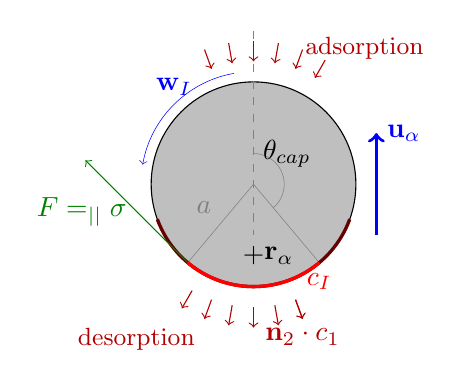
\begin{tikzpicture}[scale =1.3]
        \draw[fill=lightgray](0,0) circle (1);
        \draw[very thin,gray](230:1)--(0,0)node[midway,above left]{$a$}--(310:1);
        \draw[very thin,gray](0,0)++(310:0.3) arc (-50:90:0.3)node[right,black]{$\theta_\text{cap}$};
        \draw[very thin,blue,->](0,0)++(100:1.1) arc (100:170:1.1)node[midway,above]{$\textbf{w}_I$};
        \draw[very thick,red!40!black](0,0)++(200:1) arc (200:340:1);
        \draw[very thick,red](0,0)++(230:1) arc (230:310:1)node[below]{$c_I$};
        \draw[very thick,dashed](0,0)++(0,-0.7)node{$+$}node[right]{$\textbf{r}_\alpha$};
        \draw[very thick,blue,->](1.2,-0.5)--++(0,1)node[right]{$\textbf{u}_\alpha$};
        \draw[dashed,gray](0,1.5)--++(0,-2);
        \draw[red,->,green!50!black](230:1)--++(-1,1)node[midway,left]{$F = \grad_{||} \sigma$};
        \foreach \t in {110,100,90,80,60}{
            \draw[red!70!black, ->](\t:1.4)--++(\t:-0.2);
            \draw[red!70!black, ->](\t:-1.2)--++(\t:-0.2);
        }
        \draw[red!70!black, ->](70:1.4)--++(70:-0.2)node[above right]{\small adsorption};
        \draw[red!70!black, ->](70:-1.2)--++(70:-0.2)node[below left]{\small desorption};
        \draw[red!70!black, ->](110:-1.2)--++(110:-0.2)node[below]{$\textbf{n}_2 \cdot \grad c_1$};
    \end{tikzpicture}
    \hspace{2em}
    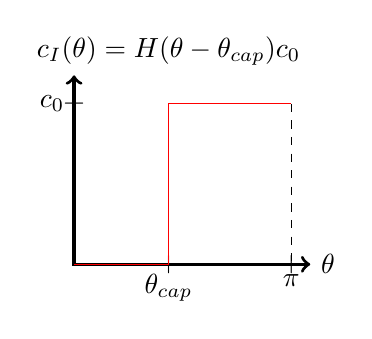
\begin{tikzpicture}[scale =1.2]
        \draw[very thick,<->](0,2)--(0,0)--(2.5,0)node[right]{$\theta$};
        \draw(1,0)node{$+$}node[below]{$\theta_{cap}$};
        \draw(1,2)node[above]{$c_I(\theta) = H(\theta- \theta_{cap}) c_0$};
        \draw[very thin,dashed](2.3,1.7)--(2.3,0);
        \draw[thin,red](0,0)--++(1,0)--++(0,1.7)--++(1.3,0);
        \draw(2.3,0)node{$+$}node[below]{$\pi$};
        \draw(0,1.7)node{$+$}node[left]{$c_0$};
    \end{tikzpicture}
    \caption{ (left) Scheme of the stagnant-cap regime of a rising contaminated bubble in a quiescent liquid. 
    (right) Hypothetical profile of the surface concentration $c_I$ in terms of the azimuthal coordinate $\theta$. }
    \label{fig:contaminated_bubbles}
\end{figure}


To derive the microscopic scale conservation equation of $c_I$ and $c_1$ we set $f_1 = c_1$ and $f_I = c_I$ in \ref{eq:dt_f_k} and \ref{eq:dt_f_I}, respectively.
Additionally, we assume that the  diffusive flux follow a Fick's law model, i.e.  $\mathbf{\Phi}_1 = D\grad c_1$ and $\mathbf{\Phi}_I = D_I\gradI c_I$,
where the constant,  $D$ and $D_I$ are the volumetric and surface diffusion coefficient, respectively.
Note that this diffusive model remains true under the assumption of dilute species concentration in both the liquid and at the interface.
\tb{The diffusive terms change in function of the regime : dilute concentration / saturated concentration, in which case $D\grad c_1 = f(c_I)$, it is worth going into that mush details ? no.}
Moreoverer, We do not consider chemical reaction or any other source term, i.e. $\textbf{S}_k = 0$ and $\textbf{S}_I=0$. 
Then, by injecting these terms in \ref{eq:dt_f_k} and \ref{eq:dt_f_I} we obtain these conservation equations : 
\begin{align}
    \pddt c_1
    + \div (\textbf{u}_1 c_1)
    &= \div (D \grad c_1)
    \;\;\; \text{in} \;\;\; \Omega_1,\\
    \pddt c_I
    + \divI (\textbf{u}_I c_I)
    &= \divI (D_I \gradI c_I)
    - (D \grad c_1)\cdot \textbf{n}_2
    \;\;\; \text{on} \;\;\; \Sigma,
    \label{eq:dt_c_I}
\end{align}
In agreement with \citet{pesci2018computational,manikantan2020surfactant}.
We recognize that the last term of \ref{eq:dt_c_I}, namely $D(\grad c_1 ) \cdot \textbf{n}_2$, turns out to be the \textit{Kinetically controlled sorption} boundary condition \citet{pesci2018computational,manikantan2020surfactant} which arise naturally in our model.
Specifically, it represents the adsorption and desorption flux between the bulk and the surface, as represented in \ref{fig:contaminated_bubbles}.
% For clarity remark that for exemple Equation (3.9) of \citet{manikantan2020surfactant} corresponds to the \textit{two-fluid} formulation of \ref{eq:dt_c_I} with a Fick's law model. 
Note that this exchange term is reduced to a contribution from the continuous phase since we assume no surfactant into the dispersed phase. 
Now that we clearly derived the microscale equation in both phases, we can easily derive the averaged equations of conservation using the hybrid model presented \ref{sec:averaged_eq}.

For a better understanding of the following equations, we now describe the steady-state kinetics that can be reached for an isolated bubble in a contaminated flow, as illustrated on \ref{fig:contaminated_bubbles}.
This will serve as a reference for the subsequent discussion.
We first assume that the transport of surfactants on the surface, represented  by the term  $\textbf{w}_I c_I$, is much greater than the other diffusive processes, such as $D\grad c_1$ and $D_I\gradI c_I$ as well as the adsorption-desorption effects. 
In this regime, the concentration of surfactant that enters from the forward-surface, due to adsorption, is advected almost instantaneously to the downward region of the particle where some of it evaporates due to desorption. 
This form an accumulation of surfactant on the downward region of the particle's surface.
At a certain point of equilibrium, the adsorption and desorption flux balance each other, leading to the steady-state kinetic of $c_I$, and the stagnant cap is stabilized to a concentration $c_0$. 
In this situation, we can consider that $c_I$ follows a constant sharp distribution along the azimuthal coordinate of the particle's surface.
Specifically, we model $c_I(\theta) = H(\theta - \theta_{cap}) c_0$ where $H$ is the Heaviside function and $\theta_{cap}$ is the angle at which the stagnant cap is formed, see \ref{fig:contaminated_bubbles}.
This assumption might seem unrealistic, nevertheless in the steady-state regime, it is approximately consistent with the observations \citep{kentheswaran2022direct}.
% In these condition the physical meaning of the first moment, $\textbf{r}_\alpha$, becomes clearer. 
From the expression of $c_I$ we deduce : $C_\alpha = \frac{c_0}{2}(1+\cos\theta_{cap})$ and $\textbf{r}_\alpha = \frac{a}{2} (\cos\theta_{cap} -1)\textbf{e}$ where $\textbf{e}$ is the unit vector in the direction of the relative velocity between the particle and the continuous phase velocity.
Thus, the knowing $\textbf{r}_\alpha$ can leads use to $\theta_{cap}$. 
This is crucial information, since the drag forces term and mass transfer closure terms are usually derived in terms of $\theta_{cap}$, such as in the following studies : \citet{sadhal1983stokes} and \citet{kentheswaran2022direct}. 

Now that the problem has been properly formulated, we can begin the derivation of the averaged equations.
The phase-averaged conservation equation for the mean concentration of surfactant in the bulk $\oneavg{c}$, is derived using \ref{eq:avg_dt_chi_f}.
It reads as,
\begin{equation}
    \pddt (\phi_1 \oneavg{c})
    + \div (\phi_1 \oneavg{c} \oneavg{\textbf{u}_1})
    = D \grad^2 (\phi_1\oneavg{c})
    - \pnavg{j_\alpha}
    +  \div \mathbf{\Sigma}_c,
    \label{eq:hybrid_avg_dt_c_1}
\end{equation}
where $j_\alpha$ is the exchange term with the dispersed phase given by,
\begin{equation*}
    j_\alpha
    =\int_{\Sigma_\alpha}
    (D\grad c_1 )
\cdot \textbf{n}_2d\Sigma,
\end{equation*}
which corresponds to the resultant of the surfactant exchange including adsorption and desorption flux.  
In the steady-state regime, when the adsorption flux balance the desorption flux,  the surfactant on the surface of the bubble can be considered as globally insoluble since $j_\alpha=0$ even through $D(\grad c_1 ) \cdot \textbf{n}_2$ may not be locally zero. 
This \textit{globally insoluble} assumption has been used in numerous studies to neglect the adsorption-desorption fluxes. 
The vector $\mathbf{\Sigma}_c$ in \ref{eq:hybrid_avg_dt_c_1}, has the following expression,
\begin{equation}
    \mathbf{\Sigma}_c
    =
     \pnavg{\textbf{J}_\alpha}
    - \pnavg{\frac{D}{a}\int_{\Sigma_\alpha}  c_1 \textbf{r} d\Sigma}
    - \phi_1\oneavg{c'_1\textbf{u}_1'},
    \label{eq:B_def}
\end{equation}
where the higher order terms have been neglected. 
The first term on the RHS of \ref{eq:B_def} corresponds to the first moment of the surfactant flux, namely $\textbf{J}_\alpha = \int_{\Sigma_\alpha} \textbf{r}
(D\grad c_1)\cdot \textbf{n}_2d\Sigma$.
It can be interpreted as the vector representing the mean direction and magnitude of the surfactant flux going in and out the surface of the droplets.
In the stagnant cap regime, this term is therefore non-zero since a mean flux is still present even through its resultant is null, i.e. $j_\alpha=0$.
In the reference frame of the particles, $\textbf{J}_\alpha$ account for the mean flux of species concentration induced by the presence of the particles, due to adsorption and desorption phenomena. 
The second term of \ref{eq:B_def} comes from the inclusion of $\phi_1$ inside the Laplacian operator in \ref{eq:hybrid_avg_dt_c_1}.
It is the first moment of $c_1$ over the droplets surface, thus it is the mean position of the continuous phase surfactant concentration over the droplet surface.
For a constant distribution $c_1$ at the bubbles interface, this vector would be zero. 
Finally, The last term of \ref{eq:B_def}, $\phi_1\oneavg{c'_1\textbf{u}_1'}$, represents the diffusive term due to the correlation of $c'_1$ with $\textbf{u}_1'$.
Overall, $\mathbf{\Sigma}_c$ is a balance between the first moment of the fluxes and the first moment of the bulk concentration, minus a contribution from the fluctuations.
Note that $\mathbf{\Sigma}_c$ appear under the divergence operator in \ref{eq:hybrid_avg_dt_c_1}, thus it will be relevant only in highly inhomogeneous cases. 
% At this stage of the research it is hard to predict the form of these closure terms. 
% Nevertheless, we know that the closure for $j_\alpha$ and $\mathbf{\Sigma}_c$ are function of the mean surface concentration $C_\alpha$ and its center of distribution $\textbf{r}_\alpha$.
% Indeed, the exchange term $\grad c_1$ which is function of the local concentration $c_I$ at surfactant saturation \citep{manikantan2020surfactant}. 
% Thus, an equation for $C_\alpha$ and a moment equation for $\textbf{r}_\alpha$ are needed. 

Regarding the equations dispersed phase, we start by the transport equation of the mean surface surfactant concentration $C_\alpha$.
From \ref{eq:avg_dt_dq_alpha_tot} the averaged conservation equation of $C_\alpha$ is straightforward to obtain and reads as,
\begin{equation}
    \pddt (\pnavg{C_\alpha})
    + \div (\pnavg{\textbf{u}_\alpha} \pnnavg{C_\alpha})
    =
    \frac{\pnavg{j_\alpha}}{s_\alpha}
    - \div (\pnavg{\textbf{u}_\alpha' C'_\alpha}).
    \label{eq:avg_dt_dC_alpha}
\end{equation}
As shown by this equation, the evolution of the mean concentration of surfactant on the particles' surface is driven by the exchange term $j_\alpha$ and the fluctuation term $\pnnavg{\textbf{u}_\alpha' C_\alpha'}$. 
The latter term is the covariance between the velocity of the particles and their mean surfactant concentration. 
It is known that the rising velocity of a bubble is greatly correlated with its mean surfactant concentration \citet{kentheswaran2022direct} thus it might be of a certain importance. 
Again, this term is under the divergence operator it will be therefore important only in non-homogeneous cases. 
Anyhow, this term must be further investigated.

We now derive an equation for the mean position of the surfactant, $\pnnavg{\textbf{r}_\alpha}$.
This is done by deriving the equation of the first moment, $s_\alpha C_\alpha \textbf{r}_\alpha$ using \ref{eq:dt_Q_alpha_tot}. 
Then, we reformulate the equation using  the relation, $\ddt (s_\alpha C_\alpha \textbf{r}_\alpha) = s_\alpha C_\alpha\ddt \textbf{r}_\alpha+ s_\alpha \textbf{r}_\alpha\ddt C_\alpha $ and  $\ddt C_\alpha = j_\alpha$. 
Finally,  we apply the average process which leads us to~:
\begin{multline}
    \pddt (\pnavg{\textbf{r}_\alpha})
    + \div (\pnavg{\textbf{u}_\alpha}\pnnavg{\textbf{r}_\alpha})
    =
    - \div (\pnavg{\textbf{u}'_\alpha\textbf{r}'_c})\\
    + \frac{n_p}{s_\alpha}\pnnavg{
        \frac{1}{C_\alpha}\left[
            \int_{\Sigma_\alpha} 
            \left[
                c_I \textbf{w}_I
                - D_I (\gradI c_I)
            \right] d\Sigma
            +\textbf{J}_\alpha
            - \textbf{r}_\alpha j_\alpha
        \right]
    }.
    \label{eq:avg_dt_dr_alpha_tot}
\end{multline}
The diffusive term $\pnavg{\textbf{u}'_\alpha\textbf{r}'_c}$ which represents the flux generated by the correlation between the mean surfactant distribution on the particles' surface and the velocity of the particles. 
Again, this term might be relevant since, as mentioned previously, the rising velocity is highly dependent on $\theta_{cap}$.
Then, the first term on the second line is the contribution of the averaged surface advection of $c_I$ along the particles' surface. 
The second term accounts for the diffusion of surfactants over the droplet surface, which acts against the formation of a sharp distribution of surfactants.
However, the contribution of this term is likely negligible based on the values of the diffusive surface coefficient, as discussed in \citet{valkovska2000determination}.
The third term of the second line, is the exchange term $\textbf{J}_\alpha$ which clearly impacts $\textbf{r}_\alpha$.
Indeed, this term accounts for the inward adsorption of concentration and downward desorption fluxes of surfactant, creating a significant disequilibrium. 
The last term, $\textbf{r}_\alpha j_\alpha$, is the contribution from the accumulation of species adsorption and desorption on the particle surface during the process driven by the three previous terms, i.e. adsorption, advection, diffusion and desorption. 
We may recognize that the latter fourth terms are being responsible for the equilibrium or not of the cap angle. 
Indeed, when all these terms are balanced, the system reaches a steady-state equilibrium for the surfactant distribution.
It is evident that in the closure of \ref{eq:avg_dt_dr_alpha_tot} one can include all properties linked to the physics of the bubbles' surface, which in turn creates a model for the surfactant distribution at first order. 

\tb{Dans cette partie il faut encore que je lise la bibliography qui existe peut etre sur ces dernière equaiton pour voir i le tout est bien coherent}

% \tb{Start : in the SSR the stagnat can is funciton of Re anfd Ma}
% Let assume that the timescale to reach the steady-state kinetic regime is much shorter than the variation of $\oneavg{c}$ seen by the particles. 
% In this situation the advection flux compensate the diffusive flux and adsorption-desorption source terms for all particles at all times.
% This equilibrium can be written :
% \begin{equation}
%     \int_{\Sigma_\alpha} 
%         c_I \textbf{w}_I
%         d\Sigma
%         - \int_{\Sigma_\alpha} 
%         D_I (\gradI c_I)
%          d\Sigma
%         +\textbf{J}_\alpha
%         = 0 
%         % - \textbf{r}_\alpha j_\alpha
%         \label{eq:steady_state_kinetic_regime}
% \end{equation}
% Nevertheless, due to a change of environment, $\oneavg{c}$ can change slowy inducing a non-zero $j_\alpha$, after what the particles reache instantaneously another steady-state kinetic regime. 
% In this situations the mean position of the surfactant is fully determined with the local concentration $\oneavg{c}$ or the local source $j_n$.
% Using the hypothesis \ref{eq:steady_state_kinetic_regime} in \ref{eq:avg_dt_dr_alpha_tot} gives the quasy steady conservation equaiton of $\textbf{r}_c$ with :
% \begin{equation}
%     \pddt (\pnavg{\textbf{r}_\alpha})
%     + \div (\pnavg{\textbf{u}_\alpha}\pnnavg{\textbf{r}_\alpha})
%     =
%     - \frac{n_p}{s_\alpha}\pnnavg{
%          \frac{\textbf{r}_\alpha j_\alpha}{C_\alpha}
%     }
%     - \div (\pnavg{\textbf{u}'_\alpha\textbf{r}'_c})
% \end{equation}
% where $\textbf{r}_\alpha$ is solely function on the local flux on the a the diffusive fluctuation term. 


As the objective of this study is not to provide a fully closed system, we will conclude the discussion on this point.
In short, this new system of equations can be used to determine the macroscopic variables $\pnnavg{C_\alpha}$ and $\pnnavg{\textbf{r}_\alpha}$, which are crucial for the closure of drag force and mass transfer in the macroscopic models.
Unfortunately, at the current state of the art, it is still challenging to derive exact closure terms for these equations, even in simplified regimes. 
However, we provided a clear methodology to derive a hybrid model tailored to the problem at hand, using the examples of surfactant transport and fiber suspension. 



\section*{Acknowledgement}
It is a great pleasure to dedicate this paper to Daniel Lhuillier whose work on the "hybrid formalism" has greatly influenced the vision of both co-authors and the present work. 
As a scientist, Daniel Lhuillier serves as a mentor for young researchers. 
He constantly challenges us to question the significance and novelty of our findings and encourages us to explore papers that the authors may have overlooked.
His constant guidance have also been a source of motivation to complete this work.
The authors are also grateful for many in-depth discussions with Professor St\'ephane Popinet as well. 

%We would like to express our sincere gratitude to Professor D. Lhuillier for his inspiring and insightful classes, which has greatly influenced our work.
%Also, the authors are grateful for many in-depth discussions with Professor St\'ephane Popinet from \textit{Institut Jean le Rond Alembert} as well. 


\appendix

\section{Proof of the generalized form of the interfacial balance law}
\label{ap:interface_proof}
% In \citet[Appendix 2]{marle1982macroscopic} they demonstrated how to obtain \ref{eq:dt_delta_I_f_I} in the specific context of the mass, momentum and energy equations. 
For completeness and ease of understanding we give in this appendix the detailed derivation of \ref{eq:dt_delta_I_f_I}. 
Let us first introduce some important relations regarding surface properties. 
Consider the arbitrary tensor $ \textbf{F}_{I}$ defined on $\Gamma(t)$.
Let us take the surface divergence of $\textbf{F}_{I||} = \textbf{F}_I \cdot (\bm\delta -\textbf{nn})$, it yields,
\begin{align}
    \delta_I \divI \textbf{F}_{I||}
    &= 
    \div (\delta_I \textbf{F}_{I||})
    - \textbf{n}(\textbf{n}\cdot\grad)\cdot (\delta_I \textbf{F}_{I||})
    - \textbf{F}_{I}\cdot\gradI\delta_I \nonumber\\
    &= 
    \div (\delta_I \textbf{F}_{I||})
    - \textbf{n}(\textbf{n}\cdot\grad)\cdot (\delta_I \textbf{F}_{I||})
    - \textbf{F}_{I} \delta_I (\textbf{n}\cdot\grad)\textbf{n}
    % &= 
    % \div (\delta_I \textbf{F}_{I||})
    \label{eq:step1}
\end{align}
were we used the chain rule and the relation $\divI(\ldots) = \div(\ldots) - \textbf{n}(\textbf{n}\cdot \grad)\cdot(\ldots)$ for the first equality. 
The second equality is derived using \ref{eq:grad_delta_I} dotted with $(\bm\delta -\textbf{nn})$, which gives the relation 
\begin{equation*}
    (\bm\delta - \textbf{nn}) \cdot \grad\delta_I
    = \gradI \delta_I
    = 
    \delta_I (\textbf{n}\cdot \grad)\textbf{n}.
\end{equation*}
Expanding the second term of \ref{eq:step1} by noticing that $\textbf{F}_{I||} = (\bm\delta - \textbf{nn})\cdot \textbf{F}_I$, and using the expression $\textbf{n}(\textbf{n}\cdot\grad)\cdot (\bm\delta - \textbf{nn}) =  (\textbf{n}\cdot\grad)\textbf{n}$
% \begin{equation*}
%     - \textbf{n}(\textbf{n}\cdot\grad)\cdot (\delta_I \textbf{F}_{I||})
%     = 
%     - \delta_I \textbf{F}_{I}\textbf{n}(\textbf{n}\cdot\grad)\cdot (\bm\delta - \textbf{nn})
%     + (\bm\delta - \textbf{nn}) \cdot \textbf{n}(\textbf{n}\cdot\grad)(\delta_I \textbf{F}_{I})
%     = \textbf{F}_{I} \delta_I (\textbf{n}\cdot\grad)\textbf{n},
% \end{equation*}
 leads us to the useful relation :
\begin{equation}
    \delta_I \divI \textbf{F}_{I||}
    = 
    \div (\delta_I \textbf{F}_{I||}). 
    \label{eq:proof_1}
\end{equation}
% Making use of the same principles one can show the already common expression  
% \begin{equation}
%     \divI
%     \textbf{F}_{I}
%     = 
%     \divI
%     \textbf{F}_{I||}
%     +(\textbf{F}_I \cdot \textbf{n})  \div \textbf{n},
% \end{equation}
% which, multiplied with $\delta_I$ gives 
% \begin{equation}
%     \delta_I \divI
%     \textbf{F}_{I}
%     = 
%     \div
%     (\delta_I \textbf{F}_{I||})
%     +\delta_I (\textbf{F}_I \cdot \textbf{n})  \div \textbf{n}. 
%     \label{eq:proof_1}
% \end{equation}


To demonstrate that \ref{eq:dt_delta_I} and \ref{eq:dt_delta_I_f_I} are consistent we must prove the equality 
\begin{equation}
    \delta_I
    \left[ \pddt f_I^0 
    + f_I^0 (\textbf{u}_{I}^0\cdot \textbf{n})  (\div \textbf{n})
    +\divI
    (f_I^0 \textbf{u}_{I||}^0
    - \mathbf{\Phi}_{I||}^0 )
    \right]
    =
    \pddt (\delta_If_I^0) 
    +\div
    (\delta_If_I^0 \textbf{u}_I^0
        - \delta_I\mathbf{\Phi}_{I||}^0 ).
    \label{eq:to_prove}
\end{equation}
This is easily done  using \ref{eq:dt_f_I} on the two first terms on the left-hand side of \ref{eq:to_prove} which gives
\begin{equation*}
    \delta_I \pddt f_I^0 
    + f_I^0 \delta_I (\textbf{u}_I\cdot\textbf{n})(\div \textbf{n})
    = 
     \pddt (f_I^0 \delta_I)
    + \div(f_I^0  \delta_I \textbf{n}(\textbf{n}\cdot\textbf{u}_I^0)). 
    % - \delta_I (\textbf{n}\cdot\textbf{u}_I^0) (\textbf{n}\cdot \grad)f_I^0. 
\end{equation*}
Where it is assumed that $\delta_I (\textbf{n}\cdot\textbf{u}_I^0)(\textbf{n}\cdot\grad) f_I^0 = 0$ for reasons discussed in detailed in \citet{orlando2023evolution,estrada1985distributional}. 
Then, using the relation \ref{eq:proof_1} on the remaining terms on the left-hand side of \ref{eq:to_prove} directly proves \ref{eq:to_prove} and by extension \ref{eq:dt_delta_I_f_I}. 





\section{Arbitrary order moments equation}
\label{ap:Moments_equations}

Let's define the arbitrary moment of the tensor $f$, by, 
\begin{equation*}
    Q_{i_1\ldots i_n}
    = \int_{V_\alpha} 
    \pri{1}{n} f dV
\end{equation*}
Then,
\begin{multline*}
    \ddt Q_{i_1\ldots i_n}
    =\int_{V_\alpha} \left[ \partial_t \left(\pri{1}{n}f\right) 
    + \partial_k \left(u_k \pri{1}{n}f\right) \right]dV\\
    +\int_{S_\alpha} \pri{1}{n} f \left(u^I_k - u_k\right) n_k dS.
\end{multline*}
Using the product rule on the derivatives yields, 
\begin{multline*}
    \ddt Q_{i_1\ldots i_n}
    =\int_{V_\alpha} f \left[ \partial_t \left(\pri{1}{n}\right) 
    + u_k \partial_k \left( \pri{1}{n}\right) \right]dV\\
    +\int_{V_\alpha} \pri{1}{n} \left[ \partial_t \left(f\right) 
    +  \partial_k \left(u_k f \right) \right]dV\\
    +\int_{S_\alpha} \pri{1}{n} f \left(u^I_k - u_k\right) n_k dS.
\end{multline*}
From similar arguments as before one can easily show that, 
\begin{multline*}
    \ddt Q_{i_1\ldots i_n}
    = \sum_{e=1}^{n} \int_{V_\alpha} f  \prod^{n}_{\substack{ m=1 \\   m \neq e}} r_{i_m} w_{i_e}dV
    +\int_{V_\alpha} \pri{1}{n} \nablabh\cdot\mathbf{\Phi} dV\\
    + \int_{V_\alpha} \pri{1}{n} \textbf{S} dV
    +\int_{S_\alpha} \pri{1}{n} f \left(u^I_k - u_k\right) n_k dS.
\end{multline*}
The second term can be reformulated such as,
\begin{align*}
    \int_{V_\alpha} \pri{1}{n} \nablabh\cdot\mathbf{\Phi} dV
    &= \int_{S_\alpha} \nablabh \cdot \left(\pri{1}{n} \mathbf{\Phi} \right)dV
    - \int_{V_\alpha} \mathbf{\Phi} \cdot \nablabh \left(\pri{1}{n} \right)dV\\
    &= \int_{S_\alpha} \pri{1}{n} \mathbf{\Phi} \cdot \textbf{n}dS
    -\sum_{e=1}^{n} \int_{V_\alpha} \mathbf{\Phi}  \prod^{n}_{\substack{ m=1 \\m \neq e}} r_{i_m}  dV
\end{align*}
Including this relation into the former equation yields, 
\begin{multline*}
    \ddt Q_{i_1\ldots i_n}
    = \sum_{e=1}^{n} \int_{V_\alpha} \prod^{n}_{\substack{ m=1 \\   m \neq e}} r_{i_m} (w_{i_e}f  - \Phi)dV
    +\int_{S_\alpha} \pri{1}{n} \mathbf{\Phi} \cdot \textbf{n}dS\\
    + \int_{V_\alpha} \pri{1}{n} \textbf{S} dV
    +\int_{S_\alpha} \pri{1}{n} f \left(u^I_k - u_k\right) n_k dS.
\end{multline*}
Then it is possible from this equation to carry out a particular average but also to get the local scale equations. 
Indeed, if we consider $V_\alpha$ as being a fixed control volume the above equality can be rewritten such as, 
\begin{multline}
    \pddt \left(\pri{1}{n}f\right)
    + \nablabh \cdot \left(\pri{1}{n}f \textbf{u}\right)
    = n  \pri{1}{n-1}  (w_{i_n}f  - \Phi)\\
    + \pri{1}{n} \textbf{S} 
    + \nablabh \cdot \left( \pri{1}{n} \mathbf{\Phi} \right)
    \label{ap:eq:dt_Q_alpha_n}
\end{multline}


% \section{Single-particle conditional average}
\label{ap:conditional_avg}

This Appendix is dedicated to the demonstration of \ref{eq:f_exp_delta} and \ref{eq:f_exp_chi} which have surprisingly never been demonstrated for arbitrarily shaped particles.


An other notation says, 
\begin{align}
    \avg{\chi_d f_d^0}[\textbf{x},t]
    =
    \int 
    \avg{
        \delta(\textbf{x}_\alpha - \textbf{y})
        (\chi_\alpha
        f_d^0)[\textbf{x},\FF,t]
    }
     d\textbf{y}. 
\end{align}
% On the other hand we have, 
% \begin{align}
%     \pavg{\text q_\alpha}[\textbf{x},t]
%     &= 
%     \avg{\delta(\textbf{x}_\alpha - \textbf{x})\int_{\Omega_\alpha[\FF,t]} f_d^0[\textbf{y},t,\FF] d\textbf{y} }[\textbf{x},t]\\
%     &= 
%     \int \avg{\delta(\textbf{x}_\alpha - \textbf{x}) (\chi_\alpha f_d^0)[\textbf{y},t,\FF]  }d\textbf{y}\\
%     \pavg{\textbf{q}^{(1)}_\alpha}[\textbf{x},t]
%     &= 
%     \int \textbf{r} \avg{\delta(\textbf{x}_\alpha - \textbf{x}) (\chi_\alpha f_d^0)[\textbf{y},t,\FF]  }d\textbf{y}
% \end{align}
Since  $\textbf{x} = \textbf{x}_\alpha + (\textbf{x} - \textbf{x}_\alpha) = \textbf{x}_\alpha + (\textbf{x} - \textbf{y}) = \textbf{x}_\alpha + \textbf{r} $, since $\textbf{x}_\alpha = \textbf{y}$ due to the presence of the Dirac delta function,  and we defined $\textbf{y} = \textbf{x}+\textbf{r}$. 
Thus, we may write without approximation the relation, 
\begin{align}
    \avg{\chi_d f_d^0}[\textbf{x},t]
    =
    \int 
    \avg{
        \delta(\textbf{x}_\alpha - \textbf{y})
        (\chi_\alpha
        f_d^0)[\textbf{x}_\alpha + \textbf{r},\FF,t]
    }
     d\textbf{r}. 
\end{align}
Since the second distribution is not in the same phase space than the first this works. 

By taking the Taylor expansion on the Dirac Delta function we show, 
\begin{align}
    \delta(\textbf{x}_\alpha - \textbf{x} - \textbf{r})
    = 
    \delta(\textbf{x}_\alpha - \textbf{x})
    - \textbf{r} \cdot \grad\delta(\textbf{x}_\alpha - \textbf{x})
    + \ldots
    % \\
    % (\chi_\alpha f_d^0)[\textbf{y} - \textbf{r},\FF,t]
    % = 
    % (\chi_\alpha f_d^0)[\textbf{y},\FF,t]
    % - \textbf{r} \cdot \grad (\chi_\alpha f_d^0)[\textbf{y},\FF,t]
    % + \ldots
\end{align}
An other notation says, 
\begin{align}
    \avg{\chi_d f_d^0}[\textbf{x},t]
    =
    \avg{
        \delta(\textbf{x}_\alpha - \textbf{x})
        \int 
        (\chi_\alpha
        f_d^0)[\textbf{x}_\alpha + \textbf{r},\FF,t]
        d\textbf{r}. 
    }
    -\div
    \avg{ 
        \delta(\textbf{x}_\alpha - \textbf{x})
        \int 
        \textbf{r}
        (\chi_\alpha
        f_d^0)[\textbf{x}_\alpha+\textbf{r},\FF,t]
        d\textbf{y}. 
    }+\ldots
\end{align}
which is indeed equivalent to \ref{eq:f_exp_chi}. 

For surface quantities we apply the same reasoning, namely we write, 
\begin{align}
    \avg{\delta_\Gamma f_\Gamma^0}[\textbf{x},t]
    =
    \int 
    \avg{
        \delta(\textbf{x}_\alpha - \textbf{y})
        (\delta_\Gamma f_\Gamma^0)[\textbf{x},\FF,t]
    }
     d\textbf{y}. 
\end{align}
swhitching $\textbf{x}$ by $\textbf{x}_\alpha+\textbf{r}$ and carrying out the taylor expansion on the Dirac delta function gives, 
\begin{align}
    \avg{\chi_d f_d^0}[\textbf{x},t]
    =
    \avg{
        \delta(\textbf{x}_\alpha - \textbf{x})
        \int 
        (\delta_\Gamma f_\Gamma^0)[\textbf{x}_\alpha + \textbf{r},\FF,t]
        d\textbf{r}. 
    }
    -\div
    \avg{ 
        \delta(\textbf{x}_\alpha - \textbf{x})
        \int 
        \textbf{r}
        (\delta_\Gamma f_\Gamma^0)[\textbf{x}_\alpha+\textbf{r},\FF,t]
        d\textbf{y}. 
    }+\ldots
\end{align}
which proves \ref{eq:f_exp_chi}. 

% \input{The_hybride_model/conditional_eq_notes.tex}
% \section{Introduction to the closure problem}
\label{ap:Closure_problem}

The closure terms in the above equation are the results of the ensemble average operator $\avg{\ldots}$. 
In all rigor, we cannot compute theoretically such an average since it necessitates knowing the distribution $P(\FF)$ and the exact expression of the local terms indicated by the notation $(\ldots)^0$. 
In the same spirit as in \citet{batchelor1972sedimentation,hinch1977averaged} and \citet{zhang1994averaged} we demonstrate here that it is therefore necessary to reformulate the closure term to remove the ensemble average procedure. 
We demonstrated in \ref{ap:Closure_problem} that any ensemble-averaged quantities can be reformulated as an integral of what we call \textit{conditionally-averaged quantities}. 
The expressions obtained are  consistent with \citet{batchelor1972sedimentation,hinch1977averaged} and \citet{zhang1994averaged} which also proposed conditional averages, but somewhat more general. 
In a second step, we demonstrate how to derive what we call the \textit{conditionally-averaged equations} that are needed to obtain the \textit{conditionally-averaged quantities}. 
For example, in \citet{kim1985modelling} they use the \textit{conditionally-averaged equations} to consider the effect of finite volume fraction on the drag force closure term, in fixed beds of spherical solid spheres. 
Again our derivation is directly inspired by the cited author, but the approach is generalized in many ways. 
For instance, in dilute and low Reynolds number assumption these equations correspond to the classic problem of the disturbance field generated by a translating droplet in an otherwise quiescent liquid flow. 
The real interest behind this demonstration is that it is kept general and offers many possibilities for model extension.
While more complicated considerations cannot be usually solved theoretically, these general formulations extend our current understanding of the closure problem. 


In \ref{sec:reformulation} and \ref{sec:the_disturbance_eq} we discuss the general approach to derive the closure problem, while in \ref{sec:application} we derive the closures terms of the momentum and energy equations. 
Since the derivation of the closure terms can be understood through physical arguments, readers who are less interested in the rigorous mathematical formulation of the closure problem, which can be quite involved, may skip directly to \ref{sec:application}.


\section{Reformulation of the closure terms}
\label{sec:reformulation}

Our final objective will be to compute our closures within the dilute Stokes flow regime for spherical particles of radius $a$. 
In this regime we expect that the closure terms will only be determined by the center of mass velocity of the droplets ($\textbf{u}_p$), their position in space, and the macroscopic properties of the continuous phase ($\textbf{u}_f, \grad \textbf{u}_f \ldots$). 
Indeed, as we will demonstrate in the following section, only these properties define the boundaries of the \textit{single-particle} conditionally-averaged equations, and are therefore sufficient to achieve closure of the problem  in the Stokes flow regime. 

Therefore, in the following, we express our closures in terms of averaged quantities, conditioned on the position of the center of mass of a \textit{test-particle} and its center of mass velocity. 
Note that for shape-dependent closure terms it would also be necessary to obtain the \textit{shape-conditioned} averaged fields, but this is out of the scope of this work.
  
\subsection{Interfacial terms}

In the equations presented in \ref{sec:application} certain closures, such as surface traction forces and surface heat fluxes, are expressed in the form of particle-averaged surface integrals. 
Here, we focus on reformulating these terms in terms of \textit{single-particle} conditionally-averaged quantities, which will be defined in the subsequent sections.

As the procedure is similar for all surface particle-averaged terms, let us take the example of the drag force term appearing in both averaged momentum equations (\ref{eq:dt_hybrid_rhou_f} and \ref{eq:dt_hybrid_up}). 
From the definition of the particle average we write,
\begin{align}
    \pSavg{\bm\sigma_f^0\cdot\textbf{n}}[\textbf{x},t]
    &= \avg{ \sum_{\alpha=1}^N \delta(\textbf{x}-\textbf{x}_\alpha[t; \FF])
    \int_{\Gamma_\alpha(t,\FF)}
    (\bm\sigma_f^0\cdot\textbf{n})[\textbf{y},t;\FF]
    d\Gamma[\textbf{y}] }
    \label{eq:first_step_reallay}
\end{align}
By writing this integral explicitly, we emphasize that the particle-averaged quantity (left-hand side of \ref{eq:first_step_reallay}) is evaluated at the point \textbf{x}, while the parameter $\textbf{y}$ is used for the integration over the particle's surface, which has its center of mass at \textbf{x} due to the presence of the Dirac delta. 
Thus, the notation $(\bm\sigma_f^0\cdot\textbf{n})[\textbf{y},t;\FF]$ means that we evaluate the local stress as well as the local normal $\textbf{n}$ to the particle, at \textbf{y}. 
We now enlarge the domain of integration from $\Gamma_\alpha$ (the surface of the particle $\alpha$) to $\mathbb{R}^3$ with the introduction of the interface indicator function of the particle $\alpha$, namely $\delta(|\textbf{y} - \textbf{x}_\alpha[t,\FF]| - a)$. 
It reads,
\begin{multline}
    \pSavg{\bm\sigma_f^0\cdot\textbf{n}}[\textbf{x},t]
    = \\
    \int_{\mathbb{R}^3}
    \avg{
     \sum_{\alpha=1}^N 
     \delta(\textbf{x}-\textbf{x}_\alpha[t \FF])
    \delta(|\textbf{y} - \textbf{x}_{\alpha}[t;\FF]|-a)
    (\bm\sigma_f^0\cdot\textbf{n})[\textbf{y},t;\FF]
    }
    d\textbf{y}. 
    \label{eq:first_step_drag}
\end{multline} 
Since the domain of integration $\mathbb{R}^3$ is now independent of $\FF$, we could substitute the integral and ensemble average operator. 
As mentioned above, we assume that our closure terms are entirely determined by the center of mass velocity of the particles and their position in space. 
Therefore, to include the condition on the particle velocity we introduce the relation 
\begin{equation}
    \int_{\mathbb{R}^3} \delta(\textbf{w} - \textbf{u}_\alpha[\FF,t]) d\textbf{w} = 1,
    \label{eq:Pw_normed}
\end{equation}
where $\textbf{w}$ is the test-particle center of mass velocity in the Eulerian space and $\textbf{u}_\alpha$ in the Lagrangian framework. 

Moreover, since the expression within the ensemble average in \ref{eq:first_step_drag} is identically zero when, $\textbf{x}_\alpha \neq \textbf{x}$, we may replace the interface indicator function such as   
\begin{equation}
    \delta(\textbf{x}-\textbf{x}_\alpha[t,\FF])\delta(|\textbf{y} - \textbf{x}_{\alpha}[t,\FF]|-a) = \delta(\textbf{x}-\textbf{x}_\alpha[t,\FF])\delta(|\textbf{y} - \textbf{x}|-a). 
    \label{eq:from_R3_to_S}
\end{equation}
Since the function $\delta(|\textbf{y} - \textbf{x}|-a)$ is not dependent on $\FF$ it can be taken out of the ensemble average operator, hence reducing the domain of integration from $\mathbb{R}^3$ to $|\textbf{y}-\textbf{x}| = a$ in \ref{eq:first_step_drag}. 
For deformable or non-spherical particles, this function may take a more complicated form, since the interface of a deformable or anisotropic particle is not entirely determinate by its center of mass position. 
It is clear that if the position of the interface is conditioned by the exact shape of the interface, then we can always express the interface indicator function as $\delta(f(\textbf{x}))$ where $f$ is a distance function of the shape that may depend on the particle's orientation (for anisotropic particles) or aspect ratio (for slightly deformable ones). 
Anyhow, this approach is generalizable to other kinds of particles, but in this work, we consider only spherical droplets. 

Injecting \ref{eq:Pw_normed} and \ref{eq:from_R3_to_S} in \ref{eq:first_step_drag} and using the last remark leads us to the relation 
\begin{equation}
    \pSavg{\bm\sigma_f^0\cdot\textbf{n}}[\textbf{x},t]
    =
    \int_{\mathbb{R}^3}
    P_1[\textbf{x},\textbf{w},t]
    \int_{|\textbf{x}-\textbf{y}|=a}
    (\bm\sigma_f^1 \cdot \textbf{n})[\textbf{y},\textbf{x},\textbf{w},t]
    d\textbf{y}
    d\textbf{w}
    \label{eq:conditionally_averaged}
\end{equation}
where we introduced the definitions, 
\begin{align}
    \bm\sigma^1_f[\textbf{y},\textbf{x},\textbf{w},t]
    % \phi_I^1[\textbf{y}|\textbf{x},\textbf{w},t] 
    % P_1[\textbf{x},\textbf{w},t]
    &= 
    \frac{1}{P_1}
    \avg{
    \sum_\alpha^N 
    \delta(\textbf{x} - \textbf{x}_\alpha[t,\FF])
    \delta(\textbf{w} - \textbf{u}_\alpha[t,\FF])
    % \delta(|\textbf{y} - \textbf{x}_{\alpha}[t,\FF]|-a)
    \bm\sigma_f^0[\textbf{y},t,\FF]
    },
    \label{eq:sigma_f_1}
    \\
    % \phi_I^1[\textbf{y}|\textbf{x},\textbf{w},t] 
    % P_1[\textbf{x},\textbf{w},t]\nonumber\\
    % = 
    % \avg{
    % \sum_\alpha^N 
    % \delta(\textbf{x} - \textbf{x}_\alpha[t,\FF])
    % \delta(\textbf{w} - \textbf{u}_\alpha[t,\FF])
    % \delta(|\textbf{y} - \textbf{x}_{\alpha}[t,\FF]|-a)
    % }\\
    P_1[\textbf{x},\textbf{w},t]
    &= 
    \avg{
    \sum_\alpha^N 
    \delta(\textbf{x} - \textbf{x}_\alpha[t,\FF])
    \delta(\textbf{w} - \textbf{u}_\alpha[t,\FF])
    }. 
\end{align}
% \tb{Since we reduced the surface int the stress isn't any more conditioned by the surface }
% Here $\bm\sigmais the \textit{single-particle} conditionally-averaged local stress of the continuous phase knowing that interface of the particle at $\textbf{x}$ is  present in \textbf{y} and that there is a particle at \textbf{x} with velocity \textbf{w}. 
With this definition, $\bm\sigma^1_f$ is the continuous phase stress, evaluated at $\textbf{y}$ and time $t$, averaged on every configuration where a particle is present at $\textbf{x}$ with velocity \textbf{w}, and that the point \textbf{y} is occupied by the surface of the test-particle.
% $\phi_I^1[\textbf{y}|\textbf{x},\textbf{w},t] $ is the probability of finding the interface of the particle at the location \textbf{y} knowing its center of mass is located at \textbf{x}. 
% For identical spherical particles we can write $\phi_I^1[\textbf{y}|\textbf{x},\textbf{w},t] = \delta(|\textbf{x} - \textbf{y}| -a)$.
% That is why the domain of integration over \textbf{y} in \ref{eq:conditionally_averaged} is reduced to $|\textbf{x} - \textbf{y}| < a$. 
$P_1[\textbf{x},\textbf{w},t]$ is the probability of finding a particle center of mass at \textbf{x} with velocity \textbf{w} at time $t$.
This distribution can be decomposed such that $P_1[\textbf{x},\textbf{w},t] = n_p[\textbf{x},t] P_1[\textbf{w}|\textbf{x},t]$ where $n_p$ is the number density evaluated at \textbf{x}, and $P_1$ the probability density of having a particle with velocity \textbf{w} knowing its center of mass location is \textbf{x}. 
Note that this distribution is normed 
\begin{equation*}
    \int_{\mathbb{R}^3} P_1[\textbf{w}|\textbf{x},t] d \textbf{w} = 1. 
\end{equation*}
Finally, note that in \ref{eq:conditionally_averaged} the droplet's shape and the position of its center of mass fully determine the normal vector $\textbf{n}$, allowing it to be taken outside the ensemble average. 

All quantities denoted with the superscript $^1$ refer to \textit{single-particle} conditionally-averaged quantities. 
These quantities are conditionally averaged based on the presence of a particle located at \textbf{x} with velocity \textbf{w}.
Additionally, in the following, we will use the shorthand,
\begin{equation}
    \delta_1[\textbf{x},\textbf{w},t,\FF]  \text{ for } \sum_\alpha \delta(\textbf{x} - \textbf{x}_\alpha[t,\FF]) \delta(\textbf{w} - \textbf{u}_\alpha[t,\FF]). 
\end{equation}  
Thus, we can define the \textit{single-particle} conditional-average of a local quantity $f^0$, as 
\begin{equation*}
    f^1[\textbf{y}|\textbf{x},\textbf{w},t] P_1[\textbf{x},\textbf{w},t] = \avg{\delta_1 f^0[\textbf{y},\FF,t]}.
\end{equation*}
Such that $f^1$ is the averaged value of $f^0$ at \textbf{y} over all configurations where a particle is present at \textbf{x} with velocity \textbf{w}. 
If $f_k$ is a quantity defined in the phase $k$ we may write 
\begin{equation*}
    f^1_k[\textbf{y}|\textbf{x},\textbf{w},t] \phi_k^1[\textbf{y}|\textbf{x},\textbf{w},t]  P_1 = \avg{\delta_1 \chi_k f^0_k [\textbf{y},\FF,t]}.
\end{equation*}
Such that $\phi_k^1$ is the probability of finding the phase $k$ at \textbf{y} knowing a particle is located at \textbf{w} with velocity \textbf{w}, and $f_k^1$ the conditional average of $f_k^0$. 
For example, we define the \textit{single-particle conditioned average} of the continuous phase velocity fields by, 
\begin{equation*}
    \textbf{u}_f^1 \phi_f^1 P_1
    = \avg{\delta_1 \chi_f \textbf{u}_f^0}
\end{equation*} 
where $\phi_f^1$ is the probability of finding the continuous phase at \textbf{y} knowing a particle is present at \textbf{x} with velocity \textbf{w}. 
$\textbf{u}_f^1$ is the averaged local velocity evaluated at \textbf{y} knowing the continuous phase is present at \textbf{y} with a particle at \textbf{x} having velocity \textbf{w}. 

The stress present in \ref{eq:conditionally_averaged} can now be expressed in terms of conditionally-averaged velocity and pressure fields. 
We use the constitutive law of Newtonian fluids, $\bm\sigma_f^0 = -p_f^0 \bm\delta + \mu_f [\pddy \textbf{u}_f^0+ (\pddy \textbf{u}_f^0)^\dagger]$, with $\pddy$ the gradient over the \textbf{y} coordinate.
Injecting this law into \ref{eq:sigma_f_1} we obtain directly 
\begin{equation}
    \bm\sigma_f^1
    = - p_f^1 \bm\delta
    +\mu_f [\pddy \textbf{u}_f^1+(\pddy \textbf{u}_f^1)^\dagger], 
    \label{eq:sigma_f_surf}
\end{equation}
where, we observed that $\delta_1$ is independent of \textbf{y}, meaning that it could be permuted with the gradient operator in \ref{eq:sigma_f_surf}. 
In conclusion, the ensemble averaged interphase drag force term can be expressed as the surface integral of the Newtonian stress defined based on the \textit{single-particle} conditional-averaged fields: $\textbf{u}_f^1$, and $p_f^1$. 

It must be understood that this definition \eqref{eq:sigma_f_surf} is only true because the stress is evaluated at the surface of the droplet, in the general case we have, 
\begin{equation}
    P_1 \phi_f^1 \bm\sigma_f^1
    =
    P_1 \phi_f^1 p_f^1
    +  \avg{\delta_1\chi_f \{ - p_f^0 \bm\delta + \mu_f [\pddy \textbf{u}_f^0+  (\pddy \textbf{u}_f^0)^\dagger]\}}. 
\end{equation}
From this expression, we can propose two formulations for the continuous phase stress,   
\begin{align}    
    \bm\sigma_f^1
    &= 
    - p_f^1 \bm\delta 
    + \mu_f [\pddy \textbf{u}_f^1+ (\pddy \textbf{u}_f^1)^\dagger ]
    - \frac{\mu_f }{P_1 \phi_f^1}\avg{\delta_1 \delta_\Gamma (\textbf{n}_d \textbf{u}_f''+  \textbf{u}_f'' \textbf{n}_d)},
    \label{eq:sigma_f_surf15}
    \\
    \bm\sigma_f^1
    &= 
    - p_f^1 \bm\delta 
    + \frac{\mu_f }{\phi_f^1} [\pddy \textbf{u}^1+ (\pddy \textbf{u}^1)^\dagger ]
    - \frac{\mu_f }{\phi_f^1} \phi_d^1 \textbf{e}_d^1. 
    \label{eq:sigma_f_surf2}
\end{align}
Where we have defined $\textbf{u}_f'' = \textbf{u}_f^0 - \textbf{u}_f^1$. 
Notice that the second term on the right-hand side of \ref{eq:sigma_f_surf2} vanishes for solid particles, because there are no shearing motions inside solid particles.
While the second term of \ref{eq:sigma_f_surf15} does not necessarily vanish. 
That is why the second expression is preferred for solid particles. 

% Additionally, multiplying \ref{eq:sigma_f_surf15} and \ref{eq:sigma_f_surf2} by $\phi_f^1$ and subtracting both expressions gives, 
% \begin{equation} 
%     \frac{1}{P_1}\avg{\delta_1 \delta_\Gamma (\textbf{n}_d \textbf{u}_f''+  \textbf{u}_f'' \textbf{n}_d)}
%     -  \phi_d^1 \textbf{e}_d^1
%     = 
%     [(\textbf{u}_f^1 - \textbf{u}_d^1)\pddy\phi_d^1+ \pddy \phi_d^1(\textbf{u}_f^1 - \textbf{u}_d^1) ]
%     - \phi_d^1 [\pddy\textbf{u}_d^1+  (\pddy \textbf{u}_d^1)^\dagger ]. 
% \end{equation}
% For ensemble averaged (not conditionally-averaged) quantities we can equally show that
% \begin{multline} 
%     \avg{\delta_\Gamma (\textbf{n}_d \textbf{u}_f'+  \textbf{u}_f' \textbf{n}_d)}
%     - \phi_d \textbf{e}_d
%     = 
%     +  [(\textbf{u}_f - \textbf{u}_d)\pddy\phi_d+ \pddy \phi_d(\textbf{u}_f - \textbf{u}_d) ]
%     - \phi_d [\pddy\textbf{u}_d+  (\pddy \textbf{u}_d)^\dagger ]
% \end{multline}
% Note that for solid particles this relation can directly lead us to a closure for the surface term on the left-hand side, namely
% \begin{multline} 
%     \avg{\delta_\Gamma (\textbf{n}_d \textbf{u}_f'+  \textbf{u}_f' \textbf{n}_d)}
%     = 
%     [(\textbf{u}_f - \textbf{u}_d)\pddy\phi_d+ \pddy \phi_d(\textbf{u}_f - \textbf{u}_d) ]
%     - \phi_d [\pddy\textbf{u}_d+  (\pddy \textbf{u}_d)^\dagger ]. 
%     \label{eq:closure_un_nu}
% \end{multline}


At the surface of the test-particle, the probability of finding the dispersed phase, i.e. finding another particle in contact with the reference particle, is identically null. 
Indeed, a thin film of continuous phase always separates the droplet's surface from its neighbors.
Therefore, we may write $\phi_d^1 = 0$ at $|\textbf{x}- \textbf{y}| =a$. 
Thus, when evaluated at the subsurface of the particle, we can use the relation $\textbf{u}_f^1 = \textbf{u}^1$ and $p_f^1 = p^1$. 
Consequently, to compute the surface stress of a particle, either the conditionally-averaged quantities of the continuous phase ($\textbf{u}_f^1, p_f^1$) or the bulk quantities ($\textbf{u}^1$, $p^1$) are required. 
Another consequence of this is that, the definitions given by, \ref{eq:sigma_f_surf15}, \ref{eq:sigma_f_surf2}, or \ref{eq:sigma_f_surf} are all consistent when evaluated at the points located on the surface of the droplet at \textbf{x}. 

\subsection{Mean fields and disturbance fields contribution}

As it is often done in the literature \citep{zhang1994ensemble,jackson2000,wang2021numerical,wang2024effect}, we would like to separate the contribution of the drag force into a contribution from the mean flow and pressure fields, and the one arising due to the disturbance velocity and pressure fields.  

\subsubsection{Definitions}

In the first place, we need to define what is a disturbance field.
Let us take the example of the conditioned velocity field, $\textbf{u}_f^1$, and its corresponding disturbance velocity field.
We first remark that,   
\begin{equation}
    \lim_{|\textbf{y}-\textbf{x}|\to\infty} 
    \textbf{u}_f^1[\textbf{y},\textbf{x},\textbf{w},t]
    =
    \textbf{u}_f[\textbf{y},t]. 
    \label{eq:lim_u_1}
\end{equation} 
This, relation means that the conditioned field, $\textbf{u}_f^1$, is equivalent to the semble-averaged velocity field $\textbf{u}_f$ when the particle at \textbf{x} is sufficiently far from the point where the velocity $\textbf{u}_f^1$ is evaluated (the point \textbf{y}). 
Note that this definition requires an infinitely large domain. 
This implies that the solutions obtained in the subsequent sections are restricted to infinitely large domains, devoid of boundary conditions.
Note that, since the particle-size scale $a$ is much smaller than the boundary length scale $L$, the boundaries can be considered as infinitely far from the point \textbf{x}, in which case \ref{eq:lim_u_1} is valid.
However, it is interesting to note that this will no longer be the case for other problems such as sediment transport for examples.
In this case, the boundary condition, i.e. the top of the particle bed and the ground, are at a distance of the same length scale as the particle-size. 

In light of \ref{eq:lim_u_1}, we define the disturbance velocity field as 
\begin{equation}
    \textbf{u}_f^{1d}
    =
    \textbf{u}_f^1 
    - 
    \textbf{u}_f. 
    \label{eq:def_u_1d}
\end{equation}
because it satisfies the definition, 
\begin{equation}
    \lim_{|\textbf{y}-\textbf{x}|\to\infty} 
    \textbf{u}_f^{1d}[\textbf{y},\textbf{x},\textbf{w},t]
    =
    \lim_{|\textbf{y}-\textbf{x}|\to\infty} 
    \{\textbf{u}_f^1[\textbf{y},\textbf{x},\textbf{w},t]
    - \textbf{u}_f[\textbf{y},t]\}
    = 0.
    \label{eq:lim_u_1d}
\end{equation} 
Thus, $\textbf{u}_f^{1d}$ tends to zero at large distances from the particle, this is thus consistent with the terminology used here, i.e. with the word ``disturbance''.
The definition \ref{eq:def_u_1d} can apply to any \textit{conditional-averaged} quantities $f^1$, we define
\begin{equation}
    \lim_{|\textbf{y}-\textbf{x}|\to\infty} 
    \{f_f^1[\textbf{y},\textbf{x},\textbf{w},t]
    - f_f[\textbf{y},t]\}
    =
    f_f^{\Delta}[\textbf{y},\textbf{x},\textbf{w},t]
    = 0.
\end{equation} 

\subsubsection{The force traction decomposition}

Using the decomposition $\bm\sigma_f^1 = \bm\sigma_f^{1d} + \bm\sigma_f$ in \ref{eq:conditionally_averaged} we finally introduce the decomposition of the drag force term as:  
\begin{align}
    \pSavg{\bm\sigma_f^0\cdot\textbf{n}}[\textbf{x},t]
    =
    n_p[\textbf{x},t]
    \int_{|\textbf{x}-\textbf{y}|=a}
    \bm\sigma_f[\textbf{y},t]
    \cdot \textbf{n}
    d\textbf{y}\\
    + 
    \int_{\mathbb{R}^3}
    P_1[\textbf{x},\textbf{w},t]
    \int_{|\textbf{x}-\textbf{y}|=a}
    \bm\sigma_f^{1d}[\textbf{y},\textbf{x},\textbf{w},t]
    \cdot \textbf{n}
    d\textbf{y}
    d\textbf{w}
    \label{eq:general_partition}
\end{align}
where the first term represents the contribution from the mean continuous phase stress, $\bm\sigma_f$, and the second term is the contribution from the disturbance fields stress $\bm\sigma_f^{1d}$. 
While this decomposition is arbitrary since $\bm\sigma_f^1$ could be partitioned into two other arbitrary tensors, it enables by definition, the separation of the mean flow contribution, $\bm\sigma_f$, from the drag induced by the local-scale disturbance fields, $\bm\sigma_f^{1d}$.
This decomposition is utilized by \citet[Chapter 2]{jackson2000} and \citet{zhang1997momentum,wang2021numerical,wang2024effect} for suspensions of solid spheres, although these authors do not explicitly provide the expression for the tensor $\bm\sigma_f^1$, which we aim to derive in the following sections. 

Note that $\bm\sigma_f$ is evaluated at $\textbf{y}$. 
Although $\bm\sigma_f$ is ensemble-averaged, we emphasize that it may still depend on the position in inhomogeneous flows. 
Consequently, to extract it from the integral, we recognize that $\bm\sigma_f[\textbf{y},t] = \bm\sigma_f[\textbf{x},t] + \textbf{r}\cdot \nabla\bm\sigma_f[\textbf{x},t] + \ldots$, where $\textbf{r} = \textbf{y} - \textbf{x}$. 
By retaining only the first three terms in the expansion, we can demonstrate that
\begin{equation}
    \pSavg{\bm\sigma_f^0\cdot\textbf{n}}
    =
    n_p v_p 
    \div\bm\sigma_f
    +
    \int_{\mathbb{R}^3}
    P_1
    \int_{|\textbf{x}-\textbf{y}|=a}
    \bm\sigma_f^{1d} \cdot \textbf{n}
    d\textbf{y}d\textbf{w}
    \label{eq:drag_final}
\end{equation}
Therefore, it is evident that the drag force term contains a component related to the divergence of the mean fluid-phase stress, in addition to the contribution from the disturbance fields. 
Similar arguments can be extended to the first two moments of the hydrodynamic force traction. 
This expression can be written as:
\begin{align}
    \pSavg{\textbf{r}\bm\sigma_f^0\cdot\textbf{n}}
    &=
    n_p v_p \bm\sigma_f
    +
    \int_{\mathbb{R}^3}
    P_1
    \int_{|\textbf{x}-\textbf{y}|=a}
    \textbf{r}\bm\sigma_f^{1d} \cdot \textbf{n}
    d\textbf{y}
    d\textbf{w}
    \label{eq:first_mom_general}
    \\
    \pSavg{\textbf{rr}\bm\sigma_f^0\cdot\textbf{n}}
    &=
    n_pv_p  \frac{a^2}{5} 3 [(\div \bm\sigma_f)\bm\delta]^\text{sym}
    +
    \int_{\mathbb{R}^3}
    P_1
    \int_{|\textbf{x}-\textbf{y}|=a}
    \textbf{rr}\bm\sigma_f^{1d} \cdot \textbf{n}
    d\textbf{y}
    d\textbf{w}
    \label{eq:second_mom_general}
\end{align}
where the operator $[\ldots]^\text{sym}$ returns the symmetric part of the arguments. 
It is important to note that the contribution from the mean stress in the second moment of the hydrodynamic force may become negligible for small $\phi_d$, as the term $a^2$ appears in this expression. 

According to the expressions \ref{eq:drag_final}, \ref{eq:first_mom_general}, and \ref{eq:second_mom_general}, we will need to compute the term $\bm\sigma^{1d}_f = \bm\sigma_f^1 + \bm\sigma_f$ where $\bm\sigma_f^1$ is given by \ref{eq:sigma_f_surf}. 
Regarding the mean continuous phase stress we recall that it can be written in two ways, namely 
\begin{align}
    \label{eq:mean_continuous_phase_stress}
    \bm\sigma_f
    &= - p_f \bm\delta 
    + \mu_f [\pddy \textbf{u}_f+ (\pddy \textbf{u}_f)^\dagger ]
    - \frac{\mu_f}{\phi_f}\avg{\delta_\Gamma (\textbf{n}_d \textbf{u}_f'+  \textbf{u}_f' \textbf{n}_d)}, \\
    \bm\sigma_f
    &= - p_f \bm\delta 
    + \frac{\mu_f}{\phi_f} [\pddy \textbf{u}+ (\pddy \textbf{u})^\dagger ]
    - \frac{\mu_f \phi_d}{\phi_f} \textbf{e}_d
    \label{eq:mean_continuous_phase_stress2}
\end{align}
Thus using \ref{eq:sigma_f_surf} and \ref{eq:mean_continuous_phase_stress} we find for the points on the particle's surface ($|\textbf{y}-\textbf{x}| = a$) that,
\begin{align}
    \bm\sigma_f^{1d}
    =
    - p_f^{1d} \bm\delta 
    + \mu_f [\pddy \textbf{u}_f^{1d}+ (\pddy \textbf{u}_f^{1d})^\dagger ]
    + \frac{\mu_f }{\phi_f}\avg{\delta_\Gamma (\textbf{n}_d \textbf{u}_f'+  \textbf{u}_f' \textbf{n}_d)}. 
    \label{eq:sigma_explict}
\end{align}
Thus, according to \ref{eq:sigma_explict}, the disturbance stress that is integrated over the particle surface in \ref{eq:drag_final} to \ref{eq:second_mom_general}, is not only the Newtonian stress-like contribution of the disturbance fields ($\textbf{u}_f^1$ and $p_f^1$), but also includes the contribution of the term $\avg{\delta_\Gamma (\textbf{n}_d \textbf{u}_f'+  \textbf{u}_f' \textbf{n}_d)}$. 
Thus, in the force traction closures: \ref{eq:drag_final} and \ref{eq:first_mom_general}, we will observe the appearance of the terms involving the divergence of $\avg{\delta_\Gamma (\textbf{n}_d \textbf{u}_f'+  \textbf{u}_f' \textbf{n}_d)}$ times $n_pv_p$, and  $n_pv_p \avg{\delta_\Gamma (\textbf{n}_d \textbf{u}_f'+  \textbf{u}_f' \textbf{n}_d)}$, respectively. 
These terms will ultimately cancel out their corresponding contributions in $\bm\sigma_f$ that appear on the left-hand side of \ref{eq:drag_final} and \ref{eq:first_mom_general}. 

To provide a better understanding for the following discussion we remark that for solid particles $\textbf{e}_d = 0$. 
Therefore, subtracting \ref{eq:mean_continuous_phase_stress} from \ref{eq:mean_continuous_phase_stress2}, gives directly, 
\begin{equation}
    \avg{\delta_\Gamma (\textbf{n}_d \textbf{u}_f'+  \textbf{u}_f' \textbf{n}_d)}
    = 
    (\textbf{u}_f - \textbf{u}_d)\pddy \phi_d + \pddy \phi_d (\textbf{u}_f - \textbf{u}_d)
    -  \phi_d [\pddy \textbf{u}_d+ (\pddy \textbf{u}_d)^\dagger ]. 
    \label{eq:closure_un_nu}
\end{equation} 
Therefore, at least for solid spheres, this term is non-zero as soon as there are non-negligible gradients of volume fraction and mean gradients of particle velocities. 


Thus, we conclude that the commonly used partition of the drag force, given by \ref{eq:general_partition}, does not constitute the best decomposition for this term since it requires adding the term  $\avg{\delta_\Gamma (\textbf{n}_d \textbf{u}_f'+  \textbf{u}_f' \textbf{n}_d)}$ to the classical Newtonian stresses in the second term of \ref{eq:general_partition} and subtracting it in the mean drag force term (first term of \ref{eq:general_partition}). 
This finding implies that, in the recent work of \citet{wang2021numerical, wang2024effect}, where this decomposition is employed for the drag force, we assert that they have actually computed the integral of the first two terms of \ref{eq:sigma_explict}, while neglecting the final term. 
Interestingly, \citet{wang2024effect} specifically investigates the effect of the volume fraction gradient ($\grad \phi_d$) on the drag force. 
In this context, it is clear from \eqref{eq:closure_un_nu} that the term $\avg{\delta_\Gamma (\textbf{n}_d \textbf{u}_f'+  \textbf{u}_f' \textbf{n}_d)}$ cannot be neglected. 
Only when the analysis is accurate to $\mathcal{O}(\phi_d)$ does this term vanish in \ref{eq:drag_final}, reducing \ref{eq:sigma_explict} to the Newtonian stress expression. 
Thus, the drag force computed in the DNS of \citet{wang2024effect} may not be the one defined in their momentum equations. 

Note that using \ref{eq:mean_continuous_phase_stress2} instead of \ref{eq:mean_continuous_phase_stress} in \ref{eq:sigma_explict} and switching $\textbf{u}_f^1$ and $\textbf{u}^1$ in \ref{eq:sigma_f_surf}, does not solve this inconsistency. 

\subsubsection{A better and simpler forces decomposition}

As the previous decomposition requires adding and subtracting $\avg{\delta_\Gamma (\textbf{n}_d \textbf{u}_f'+  \textbf{u}_f' \textbf{n}_d)}$ in each term of \ref{eq:general_partition}, we decide to avoid this overcomplicated operation and introduce, the partitioning 
\begin{equation}
    \bm\sigma_f^1 =
    \bm\Sigma_f + 
    \bm\Sigma_f^{1d}. 
    \label{eq:mean_Newtonian}
\end{equation}
Where the mean stress and disturbance stresses are defined as, 
\begin{align}
    \bm\Sigma_f^{1d}
    &=-p_f^{1d}\bm\delta + \mu_f^1 [\grad \textbf{u}^{1d}_f + (\grad \textbf{u}^{1d}_f)^\dagger], \\
    \bm\Sigma_f
    &=-p_f\bm\delta + \mu_f^1 [\grad \textbf{u}_f + (\grad \textbf{u}_f)^\dagger], 
\end{align}
respectively. 

Using the same methodology as in the previous manipulations we re-write the force traction closures such that, 
\begin{align}
    \pSavg{\bm\sigma_f^0\cdot\textbf{n}}
    &=
    n_p v_p 
    \div\bm\Sigma_f
    +
    \int_{\mathbb{R}^3}
    P_1
    \int_{|\textbf{x}-\textbf{y}|=a}
    \bm\Sigma_f^{1d} \cdot \textbf{n}
    d\textbf{y}d\textbf{w}
    \label{eq:drag_final2}\\
    \pSavg{\textbf{r}\bm\sigma_f^0\cdot\textbf{n}}
    &=
    n_p v_p \bm\Sigma_f
    +
    \int_{\mathbb{R}^3}
    P_1
    \int_{|\textbf{x}-\textbf{y}|=a}
    \textbf{r}\bm\Sigma_f^{1d} \cdot \textbf{n}
    d\textbf{y}
    d\textbf{w}
    \\
    \pSavg{\textbf{rr}\bm\sigma_f^0\cdot\textbf{n}}
    &=
    n_pv_p  \frac{a^2}{5} 3 [(\div \bm\Sigma_f)\bm\delta]^\text{sym}
    +
    \int_{\mathbb{R}^3}
    P_1
    \int_{|\textbf{x}-\textbf{y}|=a}
    \textbf{rr}\bm\Sigma_f^{1d} \cdot \textbf{n}
    d\textbf{y}
    d\textbf{w}
    \label{eq:second_mom_general2}
\end{align}
This decomposition, though perhaps less elegant, appears to be more physically meaningful. 
Indeed, unlike the previous approach, the mean contribution no longer depends on the mean relative motion through the term $\avg{\delta_\Gamma (\textbf{n}_d \textbf{u}_f'+  \textbf{u}_f' \textbf{n}_d)}$ in $\bm\sigma_f$ (see \ref{eq:closure_un_nu}), but solely on the mean fluid phase properties $p_f$ and $\textbf{u}_f$, while the local stress is a Newtonian-like stress.  

The main take-away of this section is that: (1)  the particle-averaged force traction terms can be computed based on the knowledge of $p_f^{1d}$ and $\textbf{u}_f^{1d}$. 
These fields can be obtained by solving the corresponding disturbance field equations. 
Notice that one may also compute the mixture properties $p^{1d}$ and $\textbf{u}^{1d}$ and then use the relation $p_f^{1d} = p^{1d} + \phi_d (p_f - p_d)$ or $\textbf{u}_f^{1d} = \textbf{u}^{1d} + \phi_d (\textbf{u}_f - \textbf{u}_d)$. 
And (2) the force decomposition often used \citep{jackson2000,zhang1997momentum,wang2021numerical,wang2024effect} seems inconsistent compared to the one computed in the cited studies.
This inconsistency is settled by re-defining the forces partition.  

\subsection{Particle phase volume terms}

Some closure terms such as the particle internal stress $\pOavg{\bm{\sigma}_2^0}$ or the particle internal dissipation term $\pOavg{\bm{\sigma}_2^0:\grad \textbf{u}_d^0}$ are particle-averaged volume integral of locals quantities. 
In this situation the reformulation is slightly different since we must consider volume and not surfaces of the particle nevertheless the approach is similar. 
For the particle internal stress we can write, 
\begin{equation}
    \pOavg{\bm\sigma_d^0}[\textbf{x},t]
    =
    \int_{\mathbb{R}^3}
    P_1[\textbf{x},\textbf{w}]
    \int_{|\textbf{x}-\textbf{y}|<a}
    \bm\sigma_d^1[\textbf{y},t;\textbf{x},\textbf{w}] 
    d\textbf{y}
    d\textbf{w}. 
    \label{eq:conditionally_averaged_vol}
\end{equation}
Assuming a Newtonian fluid for the particles, $\bm\sigma_d^0 = -p_d^0 \bm\delta + \mu_d [\nabla \textbf{u}_d^0 + (\nabla \textbf{u}_d^0)^\dagger]$, and given that within the region $|\textbf{x} - \textbf{y}| < a$, only the dispersed phase is present, allowing for the permutation between ensemble averages and derivatives, we can express this as:
\begin{equation}
    \bm\sigma_d^1  
    = 
    -p_d^1   \bm\delta
    + \mu_d  [\pddy \textbf{u}^1_d+(\pddy  \textbf{u}^1_d)^\dagger],
    \label{eq:dispersed_phase_stress}
\end{equation}
which is simply the expression of the Newtonian stress within the particle centered at \textbf{x}, based on the mean fields $p_d^1$ and $\textbf{u}_d^1$. 


\subsection{Continuous phase closures}

The closure terms of the form $\avg{\chi_f f_f^0}$ differ in their mathematical structure, as they represent an average over the continuous phase rather than the dispersed phase. 
Consequently, the reformulation method is slightly different and requires additional assumptions. Two examples of such terms are the Reynolds stress $\avg{\chi_f \textbf{u}_f'\textbf{u}_f'}$ and the fluid-phase dissipation $\avg{\chi_f \bm\sigma_f^0 : \nabla \textbf{u}_f^0}$, which appear in \ref{eq:dt_hybrid_rhou_f} and \ref{eq:dt_hybrid_k1}, respectively.  

We first notice that, 
\begin{equation}
    \frac{1}{N}\sum_\alpha^N
    \int_{\mathbb{R}^3}
    \int_{\mathbb{R}^3}
    \delta(\textbf{y}-\textbf{x}_\alpha[\FF,t])
    \delta(\textbf{w}-\textbf{u}_\alpha[\FF,t])
    d\textbf{x}
    d\textbf{w}
    = 1,
\end{equation}
where $N$ is the total number of particles in the flow. 
Using this relation one may re-formulate the ensemble average of a continuous phase quantity as 
\begin{equation}
    \phi_f f_f[\textbf{x},t]
    = 
    \frac{1}{N}
    \int_{\mathbb{R}^3}
    \int_{\mathbb{R}^3}
    f_f^1[\textbf{x},\textbf{y},\textbf{w},t] \phi_f^1[\textbf{x}|\textbf{y},\textbf{w},t]  P_1[\textbf{y},\textbf{w}] 
    d\textbf{y} 
    d\textbf{w}
    \label{eq:conditional_averaged_fluid}
\end{equation}
where,
\begin{equation*}
    f_f^1[\textbf{x},\textbf{y},\textbf{w},t] \phi_f^1[\textbf{x}|\textbf{y},\textbf{w},t]  P_1[\textbf{y},\textbf{w}]
    =     
    \avg{
    \sum_\alpha^N 
    \delta(\textbf{y}-\textbf{x}_\alpha[\FF,t])
     \delta(\textbf{w}-\textbf{u}_\alpha[\FF,t])
    (\chi_f
    f^0_f)[\textbf{x},t;\FF]
    }.
\end{equation*}
In this expression $f_f^1[\textbf{x},t;\textbf{y},\textbf{w}]$ is the average of the local quantity $f_f^0$ evaluated at $\textbf{x}$ and time $t$ conditionally on, the presence of the continuous phase at \textbf{x}, and a particle center of mass at $\textbf{y}$ with center of mass velocity $\textbf{w}$. 
Similarly, $\phi_f^1[\textbf{x},t;\textbf{y},\textbf{w}]$ is the fluid phase volume fraction at \textbf{x} and time $t$, conditionally on the presence of a particle at $\textbf{y}$ with center of mass velocity \textbf{w}. 
Notice that for $|\textbf{x} - \textbf{y}| < a$, $\phi_f^1[\textbf{y}|t,\textbf{x},\textbf{w}] = 0$ however at, 
$\lim_{|\textbf{x} - \textbf{y}| \to \infty} \phi_f^1 = \phi_f$. 
Notice that this derivation is consistent with (2.21) and (2.22) of \citet{zhang1994ensemble} with $K = 1$. 

This, formulation remains quite general and is valid regardless of the flow regime, however, the presence of the term $N$ makes this formulation unpractical. 
Indeed, $P_1 = n_p[\textbf{y},t] P_1[\textbf{w}|\textbf{y},t]$ and $n_p[\textbf{y},t] /N = V_\Omega$, where $V_\Omega$ is the volume of the whole domain. 
Remark that substituting this relation into \ref{eq:conditional_averaged_fluid} transforms the right-hand side of this relation to a volume average over $V_\Omega$ of a property evaluated at \textbf{x} on all possible particles positions in $V_\Omega$.  
Anyhow, \ref{eq:conditional_averaged_fluid} requires macroscopic information such as $N$ and $V_\Omega$, which we do not necessarily have if our goal is to compute general closure formulation. 
This is because, contrary to particle-averaged quantities, we could not consider a contribution per particle that is holds fixed at \textbf{x}, but the action of all particles on a given property of the fluid at \textbf{x}.
In other words, the integration variable is on the particle center of mass position in \ref{eq:conditional_averaged_fluid}, while in \ref{eq:conditionally_averaged} it is on the local non-averaged properties while the particle position remains fixed. 

Consequently, we adopt the approach proposed by \citet{batchelor1972sedimentation} and reformulate \ref{eq:conditional_averaged_fluid} based on the additivity assumption. 
Thus, we postulate that $f_f^0[\textbf{x},t;\FF]$ can be subdivided into $N$ contributions, namely:  
\begin{equation}
    f_f^0[\textbf{x},t;\FF]
    = 
    \sum_i^N
    f_{f_i}^0[\textbf{x},t;\FF]
    + f_{f_0}^0[\textbf{x},t;\FF]
\end{equation}
where $f_{f_i}^0$ is the disturbance fields produced by the particle $i$ on $f_f^0$ and $f_{f_0}^0$ is the undisturbed background flow. 
This implies that $f_{f}^0 = f_{f_0}^0$ in the absence of particle in the flow. 
Under this assumption, we can write, 
\begin{equation}
    \avg{\chi_f f_f^0}[\textbf{x},t]
    = 
    \int_{\mathbb{R}^3} 
    \avg{
        \sum_i^N 
    (\chi_f f_{f_i}^0)[\textbf{x}_i + \textbf{r},t,\FF] \delta(\textbf{x} - \textbf{x}_i[\FF,t] - \textbf{r})}d\textbf{r}
    +( \phi_f f_{f_0})[\textbf{x},t]
    \label{eq:first_step_additivity}
\end{equation}
Where $\phi_f f_{f_0}[\textbf{x},t]$ is the mean background flow, and were we have used a relation similar to \ref{eq:taylor_f_d}, to reformulate the first term of \ref{eq:first_step_additivity}. 
Then, we use the Taylor expansion, $\delta(\textbf{x} - \textbf{x}_i - \textbf{r}) =\delta(\textbf{x} - \textbf{x}_i) - \textbf{r}\cdot \grad\delta(\textbf{x} - \textbf{x}_i)+ \ldots$, on the first term on the right-hand side of \ref{eq:first_step_additivity} which gives,  
\begin{align}
    \avg{\chi_f f_f^0}[\textbf{x},t]
    = 
    \phi_f f_{f_0}[\textbf{x},t]
    + 
    \int_{\mathbb{R}^6} 
    (f_{f_p}^1\phi_f^1) [\textbf{y}|\textbf{x},\textbf{w},t] P_1[\textbf{w},\textbf{x}]
    d\textbf{r}
    d\textbf{w}\\
    + 
    \div 
    \int_{\mathbb{R}^6} 
    \textbf{r}
    (f_{f_p}^1\phi_f^1) [\textbf{y}|\textbf{x},\textbf{w},t] P_1[\textbf{w},\textbf{x}]
    d\textbf{r}
    d\textbf{w}
    + \ldots
    % + \grad^n 
    % \int_{\mathbb{R}^6} 
    % \mathcal{O}(\textbf{r}^n)
    % (f_{f_p}^1\phi_f^1) [\textbf{y}|\textbf{x},\textbf{w},t] P_1[\textbf{w},\textbf{x}]
    % d\textbf{r}
    % d\textbf{w}
    \label{eq:f_f_1_def}
\end{align}
with, 
\begin{equation}
    (f_{f_p}^1 \phi_f^1) [\textbf{y}|\textbf{x},\textbf{w},t] P_1[\textbf{w},\textbf{x}]
    = 
    \avg{
    \sum_i
    \chi_f f_{f_i}^0[\textbf{x}_i + \textbf{r},t;\FF] 
    \delta(\textbf{x} - \textbf{x}_i[\FF,t])
    \delta(\textbf{w} - \textbf{u}_i[\FF,t])
    }. 
\end{equation}
In this definition $f_{f_p}^1$ is the averaged value of the disturbance fields at $\textbf{x}+\textbf{r}$, produced by the particle at $\textbf{x}$, in opposition to $f_f^1$ \eqref{eq:conditional_averaged_fluid} which is the averaged value of $f_f^0$ evaluated at \textbf{x}, conditionally on the presence of an arbitrary particle at \textbf{y}.
Assuming a situation where there is no background flow (such as in the case of segmenting particle in an otherwise inert flow), a homogeneous situation, and in the dilute limit, such that $\phi_f^1 = \phi_f$ when $|\textbf{x}-\textbf{y}|>a$ and $\phi_f^1 =0$ when $|\textbf{x}-\textbf{y}|<a$, we obtain, 
\begin{equation}
    f_f[\textbf{x},t]
    = 
    \int_{\mathbb{R}^3} 
    P_1[\textbf{x},\textbf{w}] 
    \int_{|\textbf{x}-\textbf{y}| >a} 
    f_{f_p}^1[\textbf{x}+ \textbf{r}| \textbf{x}]
    d\textbf{r}
    d\textbf{w}
    + 
    \text{Error}
    \label{eq:Batchelor2}
\end{equation}
\begin{equation}
    \text{Error}
    = 
    \int{
    \mathcal{O}(|\textbf{r}| f_{f_p}^1  n_p / L)
    } d\textbf{r}. 
    \label{eq:error0}
\end{equation}
Note that in \ref{eq:error0} we have expressed explicitly the error generated due to the Taylor expansion of the Dirac delta: $\delta(\textbf{x} - \textbf{x}_i - \textbf{r})$. 
Indeed, at the leading order we find, $\delta(\textbf{x} - \textbf{x}_i - \textbf{r}) =\delta(\textbf{x} - \textbf{x}_i) +  \mathcal{O}(|\textbf{r}|/L)$, where $L$ is the typical length of the macroscopic flow variation.
Assuming that $\text{Error}= \mathcal(\phi_d^2)$ rather than \ref{eq:error0} in \ref{eq:Batchelor2}, we find that \ref{eq:Batchelor2} is exaclty equation (2.10) of \citet{batchelor1972sedimentation}. 
\citet{batchelor1972sedimentation} uses such a formula to compute the mean fluid phase velocity at a given point in the fluid, conditionally on the presence of a particle at a certain distance from this point. 
Consequently, \ref{eq:Batchelor2} is a generalization of Eq (2.10) of \citet{batchelor1972sedimentation}, in the sense that we give an explicit expression of the``Error'' term \eqref{eq:error0} based on mathematical arguments, rather than Batchelor's physical arguments. 
Additionally, \ref{eq:f_f_1_def} is a generalization of \ref{eq:Batchelor2} when the homogeneous hypothesis, as well as the dilute hypothesis, are not assumed. 



As discussed in \citet{batchelor1972sedimentation}, the first integral in \ref{eq:f_f_1_def} may diverge if the disturbance field $f_{f_p}^1$ is unbounded, and if it does not decay rapidly enough as $|\textbf{r}|$ approaches infinity. 
We think that, in cases where $f_{f_p}^1$ does not decay sufficiently fast as $|\textbf{r}|$ increases, the ``Error'' in \ref{eq:Batchelor2} also tends to infinity since we are integrating a term proportional to $f_{f_p}^1 |\textbf{r}|$ which is even more divergent for large $|\textbf{r}|$. 
Thus, we argue that Batchelor's original formula is not accurate at $\mathcal{O}(\phi_d^2)$, but rather at $\mathcal{O}(|\textbf{r}| f_{f_p}^1  n_p / L)$, making \ref{eq:Batchelor2} unable to produce physical results when $f_{f_p}^1$ does not decay rapidly since the ``Error'' also tends to infinity in these cases. 
In cases where the first integral on the right-hand side converges, but the "Error" does not, the results must still be considered unphysical, even though it is finite. 

Note that the wake of a spherical particle in an unbounded fluid in Stokes flow, yields a velocity field $\textbf{u}_{f_p}$ proportional to  $\sim 1/|\textbf{r}|$. 
Thus, such a velocity field is a good example of a situation where: the continuous phase properties $f_{f_p}^1$ is unbounded, the first integral and the ``Error'' in \ref{eq:Batchelor2} diverge. 
In such cases, Batchelor used the famous renormalization method to circumvent these difficulties. 
Note that these problems of divergent integral could be guessed well in advance since the Taylor expansion of $\delta(\textbf{x} - \textbf{x}_i - \textbf{r})$ for a vector $\textbf{r}$ that is arbitrarily large is not convergent. 
Nevertheless, such manipulation is required to demonstrate Batchelor's original formula and its generalization given by \eqref{eq:Batchelor2}. 


Additionally, we believe that in the general case, where $f_f$ is given by \ref{eq:f_f_1_def}, it is impossible to obtain meaningfull results with the latter formula. 
Indeed, \ref{eq:f_f_1_def} requires the use of the Taylor expansion, $\delta(\textbf{x} - \textbf{x}_i - \textbf{r}) =\delta(\textbf{x} - \textbf{x}_i) - \textbf{r}\cdot \grad\delta(\textbf{x} - \textbf{x}_i)+ \ldots + \mathcal{O}(\textbf{r}^n/L^n)$. 
Additionally, in the integrals of \ref{eq:f_f_1_def}, \textbf{r} is evaluated from the particle center to an infinitely large distance from it.
Thus, it is evident that for any unbounded $f_{f_p}^1$, when $|\textbf{r}| \to \infty$, there is always an arbitrary integer $n$ for which, $\int f_{f_p}^1 \phi^1_f \textbf{r}^n d\textbf{r} \to \infty$.
Thus, if one considers a sufficiently high order moment in \ref{eq:f_f_1_def}, he will end up including a divergent integral. 
Following the same argument we can show that the  ``Error'' term included due to the Taylor expansion, proportional to $\mathcal{O}(f_{f_p}^1 r^n /L^n)$ might diverge as well since $r$ goes to infinity and $L$ stays constants. 
Consequently, in the inhomogeneous situations, and for unbounded functions $f_{f_p}^1$, we state that \ref{eq:f_f_1_def} is nonphysical as it produces divergent integral and an infinite ``Error'' as well. 
 
In conclusion, \ref{eq:Batchelor2}  is meaningful only for fields that respect the following conditions: 
(1) The influence of the particles on the field $f_f^0$ must be additive, this is the case when ${f_f^0}$ follows the Stokes equations; 
(2) The closures must be derived in a homogeneous flow, such that the higher moments in \ref{eq:f_f_1_def} cancel exactly. 
And (3), the integral over $\mathbb{R}^3$ of the term $|\textbf{r}| f_{f_p}^1$ must be finite, such that \ref{eq:Batchelor2} remains finite. 
Even if \ref{eq:Batchelor2} is not ideal, we will be using this relation to compute the continuous phase closures since for instance, this is the only tool that we have. 
Note that a new method will be presented in \ref{chap:pseudoturbulence} where we use \textit{The Nearest particle statistics} \citep{zhang2021ensemble} to compute these kinds of ensemble-averaged terms, but without the need for such approximations.


\section{The single-particle ensemble averaged problem}
\label{sec:the_disturbance_eq}

Now that we linked the ensemble-averaged closures and the conditional averaged quantities, it is time to derive these conditional averaged quantities. 
Specifically, we want to find $\textbf{u}^1$ and $p^1$ or $\textbf{u}^{1d}$ and $p^{1d}$. 
To that end, we follow \citep{zhang1994averaged} and derive the \textit{single-particle} conditioned Navier-Stokes equations. 

We first recall the \textit{single-fluid} formulation of the mass and momentum at the local scale, it yields
\begin{align}
    \div \textbf{u}^0 = 0 \\
    \pddt (\rho^0\textbf{u}^0)
    + \div (\rho^0\textbf{u}^0\textbf{u}^0 - \bm\sigma^0)
    &= \rho^0 \textbf{g}
    \label{eq:dt_local}
\end{align}
where we recall that $\rho^0 = \chi_d \rho^d + \chi_f \rho^f$, $\textbf{u}^0 = \chi_f \textbf{u}_f + \chi_d \textbf{u}_d$ and that $\bm\sigma^0 = \bm\sigma_d + \bm\sigma_f + \bm\sigma_\Gamma$, with $\bm\sigma_{f,d}$ Newtonian stresses and $\bm\sigma_\Gamma = \gamma ( \bm\delta - \textbf{nn})$ is the surface tension contribution. 
Note that the boundary conditions at the surface of the droplets are implicitly included in the \textit{single-fluid} formulation \eqref{eq:dt_local}, however it will be useful later to recall them here, 
\begin{align}
    \label{eq:dt_rho_I3}
    \textbf{u}_f^0 = \textbf{u}_d^0 = \textbf{u}_\Gamma^0, \\
    \Jump{\bm{\sigma}_k^0} 
    =
    -\gamma\textbf{n}(\div \textbf{n}). 
    \label{eq:dt_rho_I2}
\end{align}

To obtain an equation for the disturbance velocity fields $\textbf{u}^{1d}$ we first notice that this field can be defined by the operation, 
\begin{equation}
    \avg{(\delta_1 - P_1) \textbf{u}^0}
    =
    P_1 \textbf{u}^1
    - P_1 \textbf{u}
    = P_1 \textbf{u}^{1d}. 
    \label{eq:first_step_u0}
\end{equation}
Note that $\textbf{u}^0$ and \ref{eq:dt_local} are evaluated at the point \textbf{x} while the Dirac function, $\delta_1(\textbf{y},\textbf{w},t,\FF) = \sum_i^N \delta(\textbf{x}_i-\textbf{y})\delta(\textbf{u}_i - \textbf{w})$ express the condition of having a particle at \textbf{y} with velocity \textbf{w}, and is therefore independent of \textbf{x}. 
From \ref{eq:first_step_u0}, we deduce that the momentum conservation equation for $\textbf{u}^{1d}$ is obtained by multiplying \ref{eq:dt_local} by $\delta_1 - P_1$ and averaging over all configurations. 
However, since $\delta_1$ is a function of time $t$, this operation will require a conservation equation for $\delta_1$ and $P_1$ as well.  

Taking the partial time derivative of $\delta_1$ yields directly, 
\begin{equation}
    \pddt\delta_1 
    + \pddy\cdot(\textbf{w}\delta_1)
    + \pddw\cdot(\textbf{a}_i\delta_1)
    = 0 
    \label{eq:dt_delta_1}
\end{equation}
where $\textbf{a}_i[\FF,t] = \pddt \textbf{u}_i[\FF,t]$ is the acceleration of the particle $i$ in the configuration $\FF$. 
Averaging this equation yields an equation for  $P_1[\textbf{x},\textbf{w},t]$ it gives, 
\begin{equation}
    \pddt P_1
    + \pddy\cdot[\textbf{w} (\delta_1 - P_1)]
    + \pddw\cdot[\delta_1 \textbf{a}_i - \textbf{a}_p P_1]
    = 0.
    \label{eq:dt_P_1}
\end{equation}
These two equations must be regarded as conservation equations of the one point statistics: $P_1$,  along its phase space formed by $\textbf{y},\textbf{w},t$. 
Note that integrating \ref{eq:dt_P_1} over $\textbf{w}$ yields a conservation equation for the number density $n_p[\textbf{y},t]$, because of \ref{eq:Pw_normed}.  

\subsection{The single-particle ensemble-averaged Navier-Stokes equations}

Multiplying \ref{eq:dt_local} by $(\delta_1 - P_1)$ and using \ref{eq:dt_delta_1},  \ref{eq:dt_P_1} yields the general form of the \textit{single-particle} conditionally-averaged \textit{single-fluid} formulation of the Navier-Stokes equations, namely,  
\begin{align}
    \div \avg{(\delta_1 - P_1) \textbf{u}^0}
    = 0 
    \label{eq:conditional_eqs_mass}
    \\
    \pddt \avg{(\delta_1 - P_1)\rho^0 \textbf{u}^0}
    + \div \avg{(\rho^0 \textbf{u}^0 \textbf{u}^0 - \bm\sigma^0 )(\delta_1 - P_1)} \nonumber \\ 
    + \pddy\cdot \avg{(\delta_1 - P_1)\rho^0 \textbf{u}^0 \textbf{w}}
    + \pddw\cdot \avg{(\delta_1\textbf{a}_i - P_1\textbf{a}_p)\rho^0 \textbf{u}^0}
    = \avg{(\delta_1 - P_1 ) \rho^0 \textbf{g}}
    \label{eq:conditional_eqs}
\end{align}
We can observe that the only differences with \ref{eq:conditional_eqs} and \ref{eq:conditional_eqs_mass} and their local counterpart is the presence of the factor $(\delta_1 - P_1)$ in front of all the terms and the additional advecting terms on the left-hand side of \ref{eq:conditional_eqs}. 
For purpose of understanding it is useful to reformulate the terms present in \ref{eq:conditional_eqs} and \ref{eq:conditional_eqs_mass}, they read
\begin{align}
    \label{eq:examples1}
    \avg{(\delta_1 - P_1) \textbf{u}^0}
    &= P_1 \textbf{u}^{1d},\\ 
    \avg{(\delta_1 - P_1)\rho^0 \textbf{g}}
    &= P_1 \rho^{1d} \textbf{g}\\
    \avg{(\delta_1 - P_1)\rho^0 \textbf{u}^0}
    &= P_1 (\rho^1 \textbf{u}_m^1 -\rho \textbf{u}_m)
    = P_1 (\rho^{1d} \textbf{u}_m^{1d} +\rho^{1d} \textbf{u}_m+\rho \textbf{u}_m^{1d}),\\
    \avg{(\delta_1 - P_1) \bm\sigma^0} 
    &= 
    P_1 \bm\sigma^{1d} 
    \label{eq:examples}
\end{align}
Where we have introduced $\rho^{1d} = \rho^1 - \rho$, which is the mean density of the mixture at \textbf{x} averaged on every configuration where a particle is present at \textbf{y}, minus the density of the whole mixture $\rho$ at \textbf{x}.  
We recall that $\textbf{u}_m = \avg{\textbf{u}^0\rho^0} / \rho$ is the Favre average of the velocity, and therefore $\textbf{u}^1_m = \avg{\textbf{u}^0\rho^0\delta_1} / (\rho^1P_1)$ is the Favre conditional average of the velocity conditioned by the presence of a particle at \textbf{y}. 
This represents the likelihood of finding the density of the mixture at \textbf{x} given that  a particle is at \textbf{y} minus the ensemble averaged mixture density.
For example, for all $|\textbf{x}- \textbf{y}| <a$  we obtain $\rho^{1d} = \rho_d - \rho_d\phi_d - \rho_f \phi_f = \phi_f (\rho_d - \rho_f)$ which when multiplied by \textbf{g} is the buoyancy.  

Although we did not explicitly write all the terms of \ref{eq:conditional_eqs} and \ref{eq:conditional_eqs_mass} we can already notice some interesting features. 
First, using \ref{eq:examples1},  \ref{eq:conditional_eqs_mass} can be written, $P_1 \div \textbf{u}^{1d} =0$, indicating that the averaged disturbance field around the partcile is divergence free.  
In \ref{eq:examples} we can observe the presence of the $\textbf{u}^{1d}$ and $\textbf{u}_m$. 
This, implies that there is a coupling between the disturbance fields $\textbf{u}^{1d}_m$, which is the local fields describing the flow around a particle (at \textbf{y}) and the mean flow variables such as the mean mixture velocity $\textbf{u}_m$.
Particularly, we can see that the total advective flux: $\avg{(\delta_1 - P_1)\rho^0 \textbf{u}^0}$,contains the product $\phi_f^{1d} \textbf{u}_m$, meaning that the ensemble averaged velocity fields $\textbf{u}_m$ will induces an additional momentum fluxes in the momentum equation of the disturbance velocity. 
As we will see in the following section, \ref{eq:conditional_eqs} is just a multiphase flow generalization of the Navier-Stokes equations written in the reference frame of an isolated particle.
Such equations are given in \citep{maxey1983equation}, where we indeed observe that the mean background ``undisturbed'' fluid velocity, is present in the advective term of the momentum equation. 

\subsection{The single-particle ensemble-averaged boundary conditions}


\ref{eq:conditional_eqs} and \ref{eq:conditional_eqs_mass} are completed by the following boundaries conditions far from the particle, 
\begin{align}
    \lim_{|\textbf{x}-\textbf{y}|\to\infty} 
    \textbf{u}^{1d}[\textbf{x},\textbf{w},\textbf{y},t] 
    = 
    \lim_{|\textbf{x}-\textbf{y}|\to\infty} 
    \textbf{u}^{1}[\textbf{x},\textbf{w},\textbf{y},t] 
    - \textbf{u}[\textbf{y},t] 
    = 0 \\
    \lim_{|\textbf{x}-\textbf{y}|\to\infty} 
    \phi_d^{1d}[\textbf{x},\textbf{w},\textbf{y},t] 
    = 
    \lim_{|\textbf{x}-\textbf{y}|\to\infty} 
    \phi_d^{1}[\textbf{x},\textbf{w},\textbf{y},t] 
    - \phi_d[\textbf{y},t] 
    = 0 \\
    \lim_{|\textbf{x}-\textbf{y}|\to\infty} 
    p^{1d}[\textbf{x},\textbf{w},\textbf{y},t] 
    = 
    \lim_{|\textbf{x}-\textbf{y}|\to\infty} 
    p^{1}[\textbf{x},\textbf{w},\textbf{y},t] 
    - p[\textbf{x},t] 
    = 0 
    \label{eq:boundary_at_infinity}
\end{align}
which basically state that the particle at \textbf{y} has no influence on the conditioned averaged field which is evaluated at \textbf{x} when $|\textbf{x}-\textbf{y}|$ is large enough. 

Note that the mean fields in \ref{eq:boundary_at_infinity} are evaluated at \textbf{x} not at the particle center \textbf{y}.
However, in the momentum equation \eqref{eq:conditional_eqs} and the boundary conditions \ref{eq:boundary_at_infinity} it will be more practical to consider these fields as constants as a function of \textbf{x}, so that they can be considered as input to our problem. 
Thus, one may replace these ensembles averaged terms by their expression at \textbf{x} using a Taylor expansion. 
At first order this yields the following boundaries condition for the conditional fields, 
\begin{align}
    % \lim_{|\textbf{x}-\textbf{y}|\to\infty} 
    \textbf{u}[\textbf{x},t] 
    &\approx \textbf{u}[\textbf{y},t] 
    + \textbf{r}\cdot \grad\textbf{u}[\textbf{y},t] 
    \label{eq:boundary_at_infinity23}
    + \ldots\\
    % \lim_{|\textbf{x}-\textbf{y}|\to\infty} 
    \phi_d[\textbf{x},t] 
    &\approx \phi_d[\textbf{y},t] 
    \label{eq:boundary_at_infinity22}
    + \textbf{r}\cdot \grad \phi_d[\textbf{y},t]  
    + \ldots\\
    % \lim_{|\textbf{x}-\textbf{y}|\to\infty} 
    p[\textbf{x},t] 
    &\approx p[\textbf{y},t] 
    + \textbf{r}\cdot  \grad p[\textbf{y},t] 
    + \ldots
    \label{eq:boundary_at_infinity2}
\end{align}
where $\textbf{r} = \textbf{x} - \textbf{y}$. 
Using \ref{eq:boundary_at_infinity2} in the boundary conditions \eqref{eq:boundary_at_infinity} we remark that they yield similar boundaries than the ones used in the problem of a moving particle immersed in an unbounded linear flow \citep{jackson1997locally,zhang1997momentum}. 
Nontheless,  \ref{eq:boundary_at_infinity} yield more general as they include a possible non-zero value for $\phi_d$. 
Thus, in non-dilute limit the particle-test cannot be considered as isolated, but immersed in an equivalent medium which has a particle volume fraction $\phi_d$ at infinity. 
Additionally, in \ref{eq:conditional_eqs}, $\phi_d[\textbf{x},t]$ appears within the expression of the mean density $\rho[\textbf{y},t]$. 
Thus, as witnessed by \ref{eq:boundary_at_infinity22}, we could also include the influence of $\phi_d$ and the mean gradient of particles concentration, $\grad \phi_d$, as input of our problem described by \eqref{eq:conditional_eqs} and \ref{eq:boundary_at_infinity}.


Additionally, the \textit{single-particle} conditionally averaged fields are all ensemble averaged on configuration where a spherical particle of radius $a$ is present at \textbf{y} with velocity \textbf{w}.
Therefore, the conditional velocity fields $\textbf{u}^1$ evaluated at any point on the surface of the particle, is given by 
\begin{equation}
    \textbf{n}\cdot \textbf{u}^1= \textbf{n} \cdot \textbf{w} \;\;\;\forall |\textbf{x} - \textbf{y}| = a. 
\end{equation}
Subtracting both side by $\textbf{u}[\textbf{x},t]$ and using \ref{eq:boundary_at_infinity2} yields
\begin{align}
    \textbf{n}\cdot\textbf{u}^{1d}
    = \textbf{n}\cdot(
    \textbf{w} 
    - \textbf{u}
    -\textbf{r} \cdot \grad\textbf{u} 
    + \ldots
    )\\
\end{align}
We recognize the classical velocity field boundary condition of a spherical droplet immersed in an arbitrary linear flow \citep{nadim}. 

The averaged stress and velocity jump conditions at the surface of the test-particle are obtained by conditionally ensemble averaging \ref{eq:dt_rho_I2} and \ref{eq:dt_rho_I3} and evaluating the resulting expressions at the points $|\textbf{x}-\textbf{y}| =a$. 
The conditional ensemble averaged stress at $|\textbf{x}-\textbf{y}| < a$ is given by \eqref{eq:stress}, and at the surface exterior of the test-particle by \ref{eq:sigma_f_surf}. 
Thus, applying the operation $\avg{\delta_1 \ldots}$ on \ref{eq:dt_rho_I2} and \ref{eq:dt_rho_I3}, and evaluating the expression at $|\textbf{x}-\textbf{y}| =a$, givesdirectly:  
\begin{align}
    \label{eq:dt_rho_I3}
    \textbf{u}_f^1 = \textbf{u}_d^1\\
    \Jump{\bm{\Sigma}_k^1} 
    =
    - \gamma\textbf{n}(\div \textbf{n}). 
    \label{eq:dt_rho_I2}
\end{align}
where we recall that $\bm{\Sigma}_k^1 = -p_k^1\bm\delta + \mu_k (\grad \textbf{u}_k^1 + (\grad \textbf{u}_k^1)^\dagger)$. 
Note that inside and at the surface exterior of the particle $\phi_d^1 = 1$ and $\phi_d^1 =0$, respectively, thus one may replace $p_k^1$ and $\textbf{u}_k^1$ by $p^1$ and $\textbf{u}^1$. 

At this stage the physical significance of the terms in \ref{eq:conditional_eqs} is not explicit. 
Nevertheless, we state that \ref{eq:conditional_eqs} corresponds to an equation for the fluid phase velocity disturbance fields, $\textbf{u}_f^{1d}$, and that \ref{eq:conditional_eqs_mass} is an equation for the disturbance fields of the fluid phase volume fraction, $\phi_f^{1d}$. 
In all generality these equations needs to be completed by a set of equations for the dispersed phases, which will be coupled with \ref{eq:conditional_eqs} and \ref{eq:conditional_eqs_mass} through the exchange term $\avg{(\delta_1 - P_1)\delta_\Gamma \bm\sigma_f \cdot \textbf{n}_d}$. 
However, as we see now, the restricted assumption made in this work allows us to neglect completely the particle phases conditionally-averaged equations. 

\tb{Does $\textbf{u}'$ depends on relative motion as suggest the BC ?? ? ?? }

\subsection{The finite particle Reynolds number dilute regime}
In the first place we consider the situation where the particle volume fraction is relatively small. 
More precisely we neglect all terms proportional to $\sim \phi_d^2$. 
To better understand what this implies notice that inside the volume of the particle, that is when $|\textbf{x}-\textbf{y}| < a$ we have $\phi_f^1 = 0$ since only the dispersed phase is presents in that area. 
However, when $|\textbf{y} - \textbf{x}| >a$ we are in the mixture phase and $\phi_f^1 \approx \phi_f$.
Therefore, neglecting the $\mathcal{O}(\phi_d^2)$ terms  implies assuming that $P_1 \phi_f \approx P_1$ and that $P_1^2 = 0$. 
Notice that $\phi_f^{1d} = -\phi_d^1 + \phi_d$ which means that $\phi_f^{1d} \sim \phi_d$ when $|\textbf{y} -\textbf{y}| > a$ therefore at  $\mathcal{O}(\phi_d^2)$ we have also $\phi_f^{1d} P_1= 0$. 
Additionally, since $\avg{\delta_\Gamma}\sim \phi_d$, we have $\avg{\delta_\Gamma(\delta_1-P_1)}\sim \phi_d^2$ if we exclude the point $\textbf{y}\in \{|\textbf{y}-\textbf{x}| = a\}$. 
Applying these considerations, we may rewrite the conditionally-averaged terms in \ref{eq:conditional_eqs} and \ref{eq:conditional_eqs_mass}  $\forall \textbf{y}\in \{|\textbf{y}-\textbf{x}| = a\}$ as, 
\begin{align*}
    \avg{(\delta_1 - P_1)\rho_f\chi_f}
    &=0 \\ 
    \avg{(\delta_1 - P_1)\rho_f\chi_f\textbf{u}^0_f}
    &= P_1 \rho_f \textbf{u}_f^{1d},\\
    % + \phi_f^{1d} \bm\sigma_f
    % + \phi_f^{1d} \bm\sigma_f^{1d} ]. 
    \avg{(\delta_1 - P_1)\rho^0\textbf{u}^0_f\textbf{u}^0_f}
    &=
    P_1\rho_f[
        \textbf{u}^{1d}_f\textbf{u}_f
        + \textbf{u}_f\textbf{u}_f^{1d}
        + \textbf{u}^{1d}_f\textbf{u}_f^{1d}
    ]
    + \avg{\delta_1\rho_f\chi_f\textbf{u}_f''\textbf{u}_f''}
    - P_1 \avg{\rho_f\chi_f\textbf{u}_f'\textbf{u}_f'}\\
    \avg{\chi_f \bm\sigma^0_f(\delta_1 - P_1)} 
    &= 
    P_1 \bm\sigma^{1d}_f 
    = 
    -P_1  p_f^{1d} 
    +P_1 \mu_f [\pddy \textbf{u}_f^{1d}+(\pddy \textbf{u}_f^{1d})^\dagger ]
\end{align*}

Using these approximations we can re-write \ref{eq:conditional_eqs} still for $|\textbf{y}-\textbf{x}| > a$, this reads,  
\begin{align}
    P_1 \pddy \cdot \textbf{u}^{1d}_f &= 0 \\
    \pddt (P_1 \rho_f \textbf{u}_f^{1d})
    + P_1 \pddy\cdot (
    \rho_f \textbf{u}^{1d}_f\textbf{u}_f^{1d} 
    + \textbf{u}_f\textbf{u}_f^{1d}
    + \textbf{u}^{1d}_f\textbf{u}_f
    + \bm\sigma^\text{Re}_f)\nonumber\\
    + \pddx\cdot (P_1 \textbf{u}_f^{1d}\rho_f\textbf{w}) 
    + \pddw\cdot \avg{(\delta_1 \textbf{a}_i- P_1 \textbf{a}_p)\rho^0\textbf{u}^0 }
    &= P_1 (
        \mu_f \pddy^2 \textbf{u}^{1d}_f  
        - \pddy p_f^{1d} 
    )
\end{align}
with, 
\begin{equation*}
    P_1\bm\sigma^{Re}_f
    = 
    % + \textbf{u}_f\textbf{u}_f^{1d}
    % + \textbf{u}^{1d}_f\textbf{u}_f^{1d}
    + \avg{\delta_1\rho_f\chi_f\textbf{u}_f''\textbf{u}_f''}
    - P_1 \avg{\rho_f\chi_f\textbf{u}_f'\textbf{u}_f'}
\end{equation*}
This is the conservative form of the dilute conditioned averaged Navier stokes equations. 
For reason that will be clear latter we would like to write the conservative form of this equation.
To do so we first notice that the averaged volume conservation equation of $\phi_f$ multiplied by $P_1$ gives, 
\begin{equation*}
    P_1\pddy \cdot \textbf{u}_f = 0.
\end{equation*}
Therefore, at $\mathcal{O}(\phi_d)$ the field $P_1\textbf{u}_f$ is divergence free, it does not imply that $\textbf{u}_f$. 
Additionally, in the dilute regime is it reasonable to assume that $\pddt P_1$ and $\pddx P_1$ are completely negligible compared to the other contributions. 
Alternatively, we may assume a complete homogeneous system such that $P_1(\textbf{x},\textbf{w},t) = P_1(\textbf{w})$. 
Under these assumptions one can write based on physical arguments that $\pddx \textbf{u}_f^{1d}[\textbf{y},\textbf{x},\textbf{w},t] = - \pddy \textbf{u}^{1d}[\textbf{y},\textbf{x},\textbf{w},t]$.
In that case, we reach the final form of the conditionally-averaged Navier-Stokes equations in the dilute regime  namely, 
\begin{align}
    \pddy \cdot \textbf{u}^{1d}_f &= 0 \\
    \rho_f \left[
        \pddt \textbf{u}_f^{1d}
        +  \textbf{u}^{1d}_f\cdot \pddy\textbf{u}_f^{1d} 
        +  \textbf{u}^{1d}_f\cdot \pddy\textbf{u}_f 
        +  (\textbf{u}_f - \textbf{w})\cdot \pddy\textbf{u}_f^{1d}
    \right]
    + \pddy \cdot \bm\sigma^\text{Re}_f
    &=
        \mu_f \pddy^2 \textbf{u}^{1d}_f  
        - \pddy p_f^{1d} 
    % + \pddw\cdot \avg{(\delta_1 - P_1)\rho^0\textbf{u}^0\textbf{a}_i}
    \label{eq:conditional_avg_eq_final}
\end{align}
with, 
\begin{equation*}
    \bm\sigma^{Re}_f
    =
    % + \textbf{u}_f\textbf{u}_f^{1d}
    % + \textbf{u}^{1d}_f\textbf{u}_f^{1d}
    + \frac{1}{P_1}\avg{\delta_1\rho_f\chi_f\textbf{u}_f''\textbf{u}_f''}
    - \avg{\rho_f\chi_f\textbf{u}_f'\textbf{u}_f'}
\end{equation*}
% and the boundary condition, 
% \begin{align*}
%     \lim_{|\textbf{y}-\textbf{x}|\to\infty} \textbf{u}_f^{1d}[\textbf{y}|\textbf{w},\textbf{x},t] = 0 \\
%     \textbf{u}_f^{1d} = \textbf{w} - \textbf{u}_f[\textbf{y},t]
%     = 
%     \textbf{w} 
%     - \textbf{u}_f|_{\textbf{y}=\textbf{x}}
%     -\textbf{r} \cdot \pddy\textbf{u}_f|_{\textbf{y}=\textbf{x}}
%     - \ldots
%     \;\;\; \forall \textbf{y} \in \{ |\textbf{y}-\textbf{x}| = a \}
%      \\
% \end{align*}
Notice that these equations are quite similar to the disturbance field equation produced by a translating particle (see for exemple equation (15) of \citet{maxey1983equation}). 
One might immediately recognize the equation (15) of \citep{maxey1983equation} which correspond to the equation for the disturbance field of an isolated translating droplets in an inertial frame. 
The only difference between equation (15) of \citep{maxey1983equation} and \ref{eq:conditional_avg_eq_final} is that we introduced the presence of an equivalent stress $\bm\sigma_f^{eq}$ related to local velocity fluctuation. 

\subsection{The stokes equation}

Noticing that the right-hand side of \ref{eq:conditional_avg_eq_final} is negligible in the Stokes flow regime. 
Thus, we finally obtain the well known system of equations describing the disturbance fields induced by an isolated particle translating in an arbitrary linear flow, that reads 
\begin{align}
    \pddy \cdot \textbf{u}^{1d}_f &= 0,  \\
    % \rho_f \left[
    %     \pddt \textbf{u}_f^{1d}
    %     +  \textbf{u}^{1d}_f\cdot \pddy\textbf{u}_f^{1d} 
    %     +  \textbf{u}^{1d}_f\cdot \pddy\textbf{u}_f 
    %     +  (\textbf{u}_f - \textbf{w})\cdot \pddy\textbf{u}_f^{1d}
    % \right]
    % + \pddy \cdot \bm\sigma^\text{Re}_f
    - \pddy p_f^{1d} 
    + \mu_f \pddy^2 \textbf{u}^{1d}_f  
    &= 0, 
    % + \pddw\cdot \avg{(\delta_1 - P_1)\rho^0\textbf{u}^0\textbf{a}_i}
    \label{eq:conditional_avg_eq_final_stokes}
\end{align}
with the boundary conditions, 
\begin{align*}
    \textbf{n}\cdot\textbf{u}^{1d}_f
    % = \textbf{n}\cdot\{\textbf{w} - \textbf{u}_f[\textbf{y},t]\}
    &= \textbf{n}\cdot\{
    \textbf{w} 
    - \textbf{u}_f[\textbf{x},t]
    -\textbf{r} \cdot \pddy\textbf{u}_f[\textbf{x},t] 
    % + \mathcal{O}(|\textbf{r}|^2)
    -\frac{1}{2}\textbf{rr} \cdot \pddy\pddy\textbf{u}_f[\textbf{x},t] + \ldots
    \},\\
    % \;\;\; \forall \textbf{y} \in \{ |\textbf{y}-\textbf{x}| = a \}. \\
    \textbf{u}^{1}_f
    &=\textbf{u}^{1}_d,\\
    [\bm\sigma^{1}_f - \bm\sigma^{1}_d ]\cdot\bm\delta_{||}
    &= 0, 
    % \;\;\; \forall \textbf{y} \in \{ |\textbf{y}-\textbf{x}| = a \}. 
\end{align*}
at on the surface of the particle, and \ref{eq:boundary_at_infinity}, at far distance from the particle. 
\tb{

\subsection{The finite volume fraction with no inertial effects}

Now we would like to study the effect of finite volume fraction on the conditionally-averaged equations. 
For purpose of simplicity we neglect all inertial terms as well as the acceleration of the particle. 
When considering the effect of non-negligible volume fraction it is easier to deal with the \textit{single-fluid} formulation of the equations. 
In this situation it can be shown that, 
\begin{align}
    P_1 \pddy \cdot \textbf{u}^{1d}
    % + \pddx\cdot (P_1 \rho_f \phi_f^{1d} \textbf{w})
    % + \pddw\cdot \avg{(\delta_1\textbf{a}_i - P_1\textbf{a}_p)\rho_f \chi_f }
    = 0 
    \label{eq:single_fluid_conditional_eqs_mass}
    \\
    % \pddt \avg{(\delta_1 - P_1)\rho_f \chi_f \textbf{u}^0_f}
     \pddy\cdot \avg{\bm\sigma^0 (\delta_1 - P_1)}
    % + \pddx\cdot \avg{(\delta_1 - P_1)\rho_f \chi_f \textbf{u}^0_f\textbf{w}}
    % + \pddw\cdot \avg{(\delta_1\textbf{a}_i - P_1\textbf{a}_p)\rho_f \chi_f \textbf{u}^0_f}
    = 0 
    \label{eq:single_fluid_conditional_eqs}
\end{align}
Notice that in this situation the disturbance velocity field $\textbf{u}_f^{1d}$ is not incompressible and follows a non-trivial transport equation.
In opposition to the bulk velocity fluid $\textbf{u}^{1d}$ which is divergence free according to \ref{eq:single_fluid_conditional_eqs_mass}.  

The  conditionally-averaged stress $\avg{\chi_f \bm\sigma^0_f (\delta_1 - P_1)}$ can be further written as, 
\begin{align*}
    \avg{\bm\sigma^0 (\delta_1 - P_1)}
    &= \avg{\chi_f \bm\sigma^0_f (\delta_1 - P_1)}
    + \avg{\chi_\Gamma \bm\sigma^0_\Gamma (\delta_1 - P_1)}
    + \avg{\chi_d \bm\sigma^0_d (\delta_1 - P_1)}\\
    &= 
    - P_1 [
        \phi_f p_f^{1d} 
        +\phi_f^{1d} p_f^{1d}
        +\phi_f^{1d} p_f 
    ]\bm\delta
    + P_1 \mu_f [\pddy \textbf{u}^{1d}+(\pddy \textbf{u}^{1d})^\dagger] \\
    &+ \avg{[\chi_d (\bm\sigma_d^0 - 2 \mu_f \textbf{e}^0_d ) + \chi_\Gamma \bm\sigma_\Gamma ]  (\delta_1 - P_1)}
\end{align*}
Additionally, the exchange term can be written such that,
\begin{multline*}
    \avg{[\chi_d (\bm\sigma_d^0) + \chi_\Gamma \bm\sigma_\Gamma ]  (\delta_1 - P_1)}\\
    \approx \avg{(\delta_1 - P_1)\delta(\textbf{x}_j - \textbf{y})\intS[j]{\textbf{r}\bm\sigma_f^0\cdot \textbf{n}}}
    -\pddy \cdot \avg{(\delta_1 - P_1)\delta(\textbf{x}_j - \textbf{y})\intS[j]{ \textbf{rr} \bm\sigma_f^0\cdot \textbf{n}}}
    + \ldots
\end{multline*}
where the summation over all the $j$ is implicit. 
Theoretically if we consider the point sufficiently far from $\textbf{x}$ we have $j\neq i$.
Thus it is the stresslet terms. 

It is clear that the above quantities shear the boundary condition, 
\begin{align*}
    \lim_{|\textbf{y}-\textbf{x}|\to\infty} 
    \textbf{u}^{1d}
    % [\textbf{y},\textbf{w},\textbf{x},t] 
    &= 
    \lim_{|\textbf{y}-\textbf{x}|\to\infty} 
    \textbf{u}^{1}
    % [\textbf{y},\textbf{w},\textbf{x},t] 
    - \textbf{u}
    = 0 
    \approx 
    \textbf{u}^{1}
    % [\textbf{y},\textbf{w},\textbf{x},t] 
    - \textbf{u} 
    -\textbf{r}\cdot\grad \textbf{u} 
    \\
    \lim_{|\textbf{y}-\textbf{x}|\to\infty} 
    \phi_f^{1d}
    % [\textbf{y},\textbf{w},\textbf{x},t] 
    &= 
    \lim_{|\textbf{y}-\textbf{x}|\to\infty} 
    \phi_f^{1}
    % [\textbf{y},\textbf{w},\textbf{x},t] 
    - \phi_f
    = 0
    \approx \phi_f^{1}
    % [\textbf{y},\textbf{w},\textbf{x},t] 
    - \phi_f
    - \textbf{r} \cdot \grad \phi_f
     \\
    \lim_{|\textbf{y}-\textbf{x}|\to\infty} 
    p^{1d}_f
    % [\textbf{y},\textbf{w},\textbf{x},t] 
    &= 
    \lim_{|\textbf{y}-\textbf{x}|\to\infty} 
    p^{1}_f
    % [\textbf{y},\textbf{w},\textbf{x},t] 
    - p_f
    = 0 \approx
    p^{1}_f
    % [\textbf{y},\textbf{w},\textbf{x},t] 
    - p_f 
    - \textbf{r}\cdot \grad p_f
    \label{eq:boundary_at_infinity}
\end{align*}
Where we have kept only the first-order  fields of the disturbance fields. 

The momentum equations is therefore, 
\begin{equation*}
    - P_1 \pddy(\phi_f p_f^{1d} + \phi_f^{1d} p_f^{1d} + \phi_f^{1d} p_f^{1d})
    + \mu_f P_1 \grad^2  \textbf{u}^{1d}
    % + \pddw\cdot \avg{(\delta_1\textbf{a}_i - P_1\textbf{a}_p)\rho_f \chi_f \textbf{u}^0_f}
    = - \avg{(\delta_1 - P_1)\delta_\Gamma \bm\sigma_f \cdot \textbf{n}_d}
\end{equation*}


}
% \section{The conditionally averaged Navier Stokes equations}
\label{ap:conditionally_navier_stokes}

In this appendix we revisit the method to derive the closure term of a stoke stain spherical droplets. 
Following \citet{zhang1994ensemble} we first demonstrate that in order to be closed the particle-averaged  fields need to be expressed in terms of \textit{single-particle} conditionally-averaged field. 
Then we demonstrate how to obtain these \textit{single-particle} conditionally-averaged field from what we call here the \textit{single-particle} conditionally-averaged equations. 

\subsection{The conditional average}
The first step is to introduce the relation between particle averaged field and \textit{single-particle} conditionally-averaged field.
For instance, let us take the example of the drag force term. 
Form the definition of the particle-average \ref{eq:p_avg} we write,
\begin{align}
    \pSavg{\bm\sigma_f^0\cdot\textbf{n}}[\textbf{x},t]
    &= \int \sum_{\alpha=1}^N \delta(\textbf{x}-\textbf{x}_\alpha[t; \FF])
    \int_{\Gamma_\alpha(t,\FF)}
    \bm\sigma_f^0\cdot\textbf{n}[\textbf{y},t;\FF]
    d\Gamma(\textbf{y}) d\PP
\end{align}
By writing this integral explicitly, we want to emphasize that the particle-averaged quantity is evaluated at the point \textbf{x}, while the integration over the surface of the particles $\alpha$ is carried out over the surface with the integration parameter $\textbf{y}$.
Therefore, we may enlarge the domain of integration from $\Gamma_\alpha$ to $\mathbb{R}^3$ by multiplying $\bm\sigma_f^0\cdot\textbf{n}(\textbf{r},t;\FF)$ with $\delta(|\textbf{y} - \textbf{x}_\alpha(t,\FF)| - a)$. 
It reads, 
\begin{equation}
    \pSavg{\bm\sigma_f^0\cdot\textbf{n}}[\textbf{x},t]
    = 
    \int_{\mathbb{R}^3}
    \int
     \sum_{\alpha=1}^N 
     \delta(\textbf{x}-\textbf{x}_\alpha(t; \FF))
    \delta(|\textbf{y} - \textbf{x}_{\alpha}(t;\FF)|-a)
    (\bm\sigma_f^0\cdot\textbf{n})[\textbf{y},t;\FF]
    d\PP
    d\textbf{y}
\end{equation}
Note that this definition is only valid for identical spherical particles of radius $a$. 
Due to the presence of $\delta(\textbf{x}-\textbf{x}_\alpha(t; \FF))$, this expression is non-zero only when $\textbf{x} = \textbf{x}_\alpha(\FF,t)$. 
Also, we can introduce the conditional average on the velocity of the particle by noticing that, 
\begin{equation*}
    \int_{\mathbb{R}^3} \delta(\textbf{c} - \textbf{u}_\alpha(\FF,t)) d\textbf{c} = 1. 
\end{equation*}
Taking in account the preceding remarks we are able to write
\begin{equation}
    \pSavg{\bm\sigma_f^0\cdot\textbf{n}}[\textbf{x},t]
    =
    n_p(\textbf{x})
    \int_{\mathbb{R}^3}
    \int_{|\textbf{x}-\textbf{y}|=a}
    \bm\sigma_f^1[\textbf{y},t;\textbf{x},\textbf{c}] \cdot \textbf{n}
    d\textbf{y}
    d\textbf{c}
    \label{eq:conditionally_averaged}
\end{equation}
where, 
\begin{equation*}
    \bm\sigma^1_f[\textbf{y},t;\textbf{x},\textbf{c}] n_p(\textbf{x},\textbf{c})
    =
    \avg{\delta_\alpha \bm\sigma^0_f}[\textbf{y},t;\textbf{x},\textbf{c}]
    = 
    \int 
    \sum_\alpha^N 
    \delta(\textbf{x} - \textbf{x}_\alpha(\FF,t))
    \delta(\textbf{c} - \textbf{u}_\alpha(\FF,t))
    \bm\sigma_f^0[\textbf{y},t;\FF]
    d\PP
\end{equation*}
is the \textit{single-particle} conditionally-averaged local stress of the continuous phase knowing that interface of the particle at $\textbf{x}$ is  present in \textbf{y}. 
In other world $\bm\sigma^1_f$ is the mean fluid phase stress evaluated at $\textbf{y}$ and time $t$ on every configuration where a particle is present at $\textbf{x}$. 
And $n_p(\textbf{x})$ is the number density but evaluated at $\textbf{x}$.
In light of \ref{eq:conditionally_averaged} we made the link between particle-average and the integral of a \textit{single-particle} conditionally-averaged quantity. 
Note that all quantities denoted with the superscript $^1$ refer to \textit{single-particle} conditionally-averaged  quantities.  
Therefore, it is implicit that these quantities are evaluated at $\textbf{y}$ and $t$ and conditionally on $\textbf{x}$. 

At some point it will also be useful to express continuous phase averaged quantities, i.e. $\avg{\chi_k f_k^0}$  in terms of one  \textit{single-particle} conditionally-averaged fields. 
Two examples are the Reynolds stress $\avg{\chi_f \textbf{u}_f'\textbf{u}_f'}$ and the fluid phase dissipation $\avg{\chi_f\sigma_f^0:\grad \textbf{u}_f^0}$ that appear in \ref{eq:dt_hybrid_rhou_f} and \ref{eq:dt_hybrid_k1}, respectively.  
To proceed one must first notice that, 
\begin{equation}
    \frac{1}{N}\sum_\alpha 
    \int_{\mathbb{R}^3}
    \int_{\mathbb{R}^3}
    \delta(\textbf{y}-\textbf{x}_\alpha)
    \delta(\textbf{c}-\textbf{u}_\alpha)
    d\textbf{x}
    d\textbf{c}
    = 1
\end{equation}
where $N$ is the total number of particle in the flow. 
Using this relation one may re-formulate the ensemble average of a continuous phase quantity as 
\begin{equation}
    f_f[\textbf{x},t]
    = 
    \frac{1}{N}
    \int_{\mathbb{R}^3}
    \int_{\mathbb{R}^3}
    f_k^1[\textbf{x},t|\textbf{y},\textbf{c}]  P_1[\textbf{y},\textbf{c}|\textbf{x},t] 
    d\textbf{y} 
    d\textbf{c}
    \label{eq:conditional_averaged_fluid}
\end{equation}
where,
\begin{equation*}
    f_k^1[\textbf{x},t|\textbf{y},\textbf{c}] P_1[\textbf{y},\textbf{c}|\textbf{x},t] \phi_k[\textbf{x},t]
    =     
    \int
    \sum_\alpha^N 
    \delta(\textbf{y}-\textbf{x}_\alpha)
     \delta(\textbf{c}-\textbf{u}_\alpha)
    \chi_k
    f^0_k[\textbf{x},t;\FF]
    d\PP.
\end{equation*}
In this expression $f_f^1[\textbf{x},t;\textbf{y},\textbf{c}]$ is the average of the local quantity $f_f^0$ evaluated at $\textbf{x}$ and time $t$ conditionally on the presence of a particle center of mass at $\textbf{y}$ with center of mass velocity $\textbf{c}$. 
% Similarly, $\phi_f^1[\textbf{x},t;\textbf{y},\textbf{c}]$ is the fluid phase volume fraction at \textbf{x} and time $t$, conditionally on the presence of a particle at $\textbf{y}$ with velocity \textbf{c}. 
Similarly, $P_1[\textbf{y},\textbf{c};\textbf{x},t]$ is the probability density of finding a particle center of mass within the infinitesimal volume $d\textbf{y}$ around $\textbf{y}$ with a center of mass velocity ranging between the interval $d\textbf{c}$ around $\textbf{c}$, knowing that the point \textbf{x} is occupied by the continuous phase. 
Notice that this derivation is consistent with (2.21) and (2.22) of \citet{zhang1994ensemble} with $K = 1$. 

In practice \ref{eq:conditional_averaged_fluid} cannot be used since $N$ is unknown. 
Instead, we use the assumption of \citet{batchelor1972sedimentation} and assume linearity of the local scale equations. 
Therefore, we stipulate that $f_f^0(\textbf{x},t;\FF)$ can be subdivided such that  
\begin{equation}
    f_f^0(\textbf{x},t;\FF)
    = 
    \sum_i
    f_{f_i}^0(\textbf{x},t;\FF)
\end{equation}
where $f_{f_i}^0(\textbf{x},t;\FF)$ is the disturbance fields produce by the particle $\alpha$ on $f_f^0$. 
This of course implies that $f_f^0 = 0$ in the absence of particle in the flow. 
Under this very restrictive hypothesis we can write, 
\begin{equation}
    \avg{\chi_ff_f^0}[\textbf{x},t]
    = 
    \sum_i
    \avg{\chi_f f_{f_i}^0(\textbf{x},t;\FF)}
    = 
    \int_{\mathbb{R}^3} 
    \avg{
        \sum_i
    \chi_f f_{f_i}^0(\textbf{x}_\alpha + \textbf{r},t;\FF) \delta(\textbf{x} - \textbf{x}_\alpha - \textbf{r})}d\textbf{r}
\end{equation}
assuming that \textbf{r} is relatively small compared to the macroscale we may write $\delta(\textbf{x} - \textbf{x}_\alpha - \textbf{r}) =\delta(\textbf{x} - \textbf{x}_\alpha) - \textbf{r}\cdot \grad\delta(\textbf{x} - \textbf{x}_\alpha)+ \ldots$
\begin{equation}
    \avg{\chi_ff_f^0}[\textbf{x},t]
    = 
    \int_{\mathbb{R}^3} 
    \phi_f^1
    f_{f_i}^1(\textbf{x}+ \textbf{r}| \textbf{x})
    n_p(\textbf{x}) 
    d\textbf{r}
\end{equation}
with, 
\begin{equation*}
    \phi_f^1 f_{f_i}^1[\textbf{x}+ \textbf{r}| \textbf{x}]n_p(\textbf{x}) 
    = 
    \int{
    \sum_i
    \chi_f f_{f_i}^0(\textbf{x}_\alpha + \textbf{r},t;\FF) \delta(\textbf{x} - \textbf{x}_\alpha)
    }d\PP
\end{equation*}
\tb{where is teh fluid phase fraction ? ? correct after }
$f_{f_i}^1[\textbf{x}+ \textbf{r}| \textbf{x}]$ is the averaged value of $f_{f_i}^0$ at $\textbf{x}+\textbf{r}$ knowing a particle is at \textbf{x} and that the point $\textbf{x}+\textbf{r}$ is occupied by the continuous phase. 
And $f_{f_i}$ is the contribution from one particle to $f_f^0$. 

At order one in the particle volume fraction 
\begin{equation}
    \avg{\chi_f f_f^0}[\textbf{x},t]
    = 
    \int_{\mathbb{R}^3} 
    % \phi_f^1
    f_{f_i}^1(\textbf{x}+ \textbf{r}| \textbf{x})
    n_p(\textbf{x}) 
    d\textbf{r}
    + \mathcal{O}({\phi^2})
\end{equation}

\subsection{The force traction term}

Let $f^1_f$ be an arbitrary \textit{single-particle} conditionally-averaged quantity. 
Notice that when $f^1_f$ is evaluated infinitely far from the particle we have the relation, 
\begin{equation*}
    \lim_{|\textbf{x} - \textbf{y}| \to \infty}  f^1_f [\textbf{y},t;\textbf{x},\textbf{c}] = f_f [\textbf{y},t]
\end{equation*}
Indeed, at large distance from a particle the \textit{single-particle} conditionally-averaged quantities are not influenced by the particles and therefore reduce to the classic averaged fields. 
Therefore, we define the distance field of a particle as $f^{1d}_f = f^1_f [\textbf{y},t;\textbf{x},\textbf{c}]  - f_f[\textbf{y},t]$ such that any disturbance field satisfy, 
\begin{equation*}
    \lim_{|\textbf{x} - \textbf{y}| \to \infty}  f^{1d}_f [\textbf{y},t;\textbf{x},\textbf{c}] = 0 
\end{equation*}
Using  $\bm\sigma_f^1 = \bm\sigma_f + \bm\sigma_f^{1d}$ these definitions we may write, 
\begin{equation}
    \pSavg{\bm\sigma_f^0\cdot\textbf{n}}[\textbf{x},t]
    =
    n_p(\textbf{x})
    \int_{\mathbb{R}^3}
    \int_{|\textbf{x}-\textbf{y}|=a}
    \bm\sigma_f
    \cdot \textbf{n}
    d\textbf{y}
    d\textbf{c}
    + n_p(\textbf{x})
    \int_{\mathbb{R}^3}
    \int_{|\textbf{x}-\textbf{y}|=a}
    \bm\sigma_f^{1d}
    \cdot \textbf{n}
    d\textbf{y}
    d\textbf{c}
    \label{eq:drag}
\end{equation}
Notice that $\bm\sigma_f$ is evaluated at $\textbf{y}$ therefore to get it out of the integration one can notice that $\bm\sigma_f(\textbf{y},t) = \bm\sigma_f(\textbf{x},t) + \textbf{r}\cdot \grad\bm\sigma_f(\textbf{x},t)+ \ldots$
where we have introduced $\textbf{r} = \textbf{y} - \textbf{x}$. 
Substituting the first two terms of this Taylor series into \ref{eq:drag} yields
\begin{equation}
    \pSavg{\bm\sigma_f^0\cdot\textbf{n}}[\textbf{x},t]
    =
    n_p v_p 
    \div\bm\sigma_f
    +
    n_p 
    \int_{|\textbf{x}-\textbf{y}|=a}
    \bm\sigma_f^{1d} \cdot \textbf{n}
    d\textbf{y}
    \label{eq:drag_final}
\end{equation}
Therefore, notice that drag force term has a component related to the mean fluid phase stress plus the contribution from the disturbance fields. 
Additionally, similar consideration can be made for the first two moments of the hydrodynamic force traction. 
This gives, 
\begin{align}
    \pSavg{\textbf{r}\bm\sigma_f^0\cdot\textbf{n}}[\textbf{x},t]
    =
    n_p v_p \bm\sigma_f
    +
    n_p 
    \int_{\mathbb{R}^3}
    \int_{|\textbf{x}-\textbf{y}|=a}
    \textbf{r}\bm\sigma_f^{1d} \cdot \textbf{n}
    d\textbf{y}
    d\textbf{c}
    \\
    \pSavg{\textbf{rr}\bm\sigma_f^0\cdot\textbf{n}}[\textbf{x},t]
    =
    n_pv_p  \frac{a^2}{5} 3 [(\div \bm\sigma_f)\bm\delta]^\text{sym}
    +
    n_p 
    \int_{\mathbb{R}^3}
    \int_{|\textbf{x}-\textbf{y}|=a}
    \textbf{rr}\bm\sigma_f^{1d} \cdot \textbf{n}
    d\textbf{y}
    d\textbf{c}
    \\
\end{align}
where the operator $[\ldots]^\text{sym}$ returns the symmetric part of the arguments.
Notice that the contribution from the mean stress in the second moment of the hydrodynamic force might become negligible for small $\phi_d$. 
In these expressions no hypothesis have been made. 


The fluid phase is a Newtonian thus, $\bm\sigma_f^0 = - p_f^0\bm\delta + 2\mu_f [\grad \textbf{u}_f^0 + (\grad \textbf{u}_f^0)^\dagger]$.
Therefore, the fluid phase stress averaged conditionally on the presence of a particle at \textbf{x} with the fluid phase at \textbf{y} might be written
\begin{align*}
    n_p \phi_f^1 \bm\sigma_f^{1d} = 
    n_p \phi_f^1 \bm\sigma_f^{1d} 
    - n_p \phi_f^1 \bm\sigma_f \\
    = - \phi_f^1 p_f^{1d}\bm\delta 
    + \mu_f \avg{\chi_f \delta_1 [\grad \textbf{u}_f^0 + (\grad \textbf{u}_f^0)^\dagger] }
    - \mu_f n_p \avg{\chi_f [\grad \textbf{u}_f^0 + (\grad \textbf{u}_f^0)^\dagger] }\\
    =- p_f^{1d}\bm\delta 
    + \mu_f \avg{(\delta_1 - n_p) [\grad \textbf{u}_f^0 + (\grad \textbf{u}_f^0)^\dagger] }
    - \mu_f \avg{\chi_d (\delta_1 - n_p) [\grad \textbf{u}_f^0 + (\grad \textbf{u}_f^0)^\dagger] }
\end{align*}
By noticing that both $\delta_1$ and $n_p$ commute with the derivatives and by noticing that  
\begin{equation*}
    \avg{(\delta_1 - n_p)  \textbf{u}^0}
    = 
    n_p \textbf{u}^{1d}
\end{equation*}
is the disturbance field of the bulk velocity conditionally on a particle present at $\textbf{y}$ we arrive at the relation 
\begin{align*}
    n_p \phi_f^1 \bm\sigma_f^{1d} = 
    - \phi_f^1 p_f^{1d} \bm\delta 
    + \mu_f n_p \left[\grad \textbf{u}^1 + (\grad \textbf{u}^1)^\dagger\right]
    - 2 \mu_f n_p \phi_d^1 \textbf{e}_d^{1d}
\end{align*}
where the second term is the contribution from the particle to the fluid phase stress, conditionally on the presence of the dispersed phase at \textbf{x} with a particle already present at \textbf{y}. 
Due to the simultaneous presence of $\phi_d$ and $n_p$ this term is negligible at first order in $\phi$. 

\subsection*{The consitional averaged Navier stokes equaiton}
As shown above $\bm\Sigma_f$ is function of the unknown of the problem so it is closed. 
The remaining term to compute is $\bm\Sigma_f^{1d}$ which is a function of $\textbf{u}_f^{1d}$ and $p_1^{1d}$. 
To obtain these fields one must solve the \textit{single-particle} conditionally-averaged equations for the disturbance fields  $\textbf{u}_f^{1d}$ and $p_1^{1d}$. 
Notice that we assume that the equation for  $\textbf{u}_f^{1d}$ and $p_1^{1d}$ follow the stokes hypothesis. 
However, in light of \ref{eq:dt_hybrid_rhou_f} the fields $\textbf{u}_f^{1}$ has no reason to follow the stokes limit hypothesis. 
For this reason we believe that (5.1) and (5.2) of \citet{zhang1997momentum} is not well posed. 

In all rigor to obtain the equations for the $\textbf{u}^{1d}$ one multiply the single-fluid formulation of the momentum \eqref{eq:dt_f} evaluated at \textbf{r} by $\sum_\alpha \delta(\textbf{x}-\textbf{x}_\alpha)$ and then average over all configuration,  and use $\textbf{u}^1 = \textbf{u}^{1d} - \textbf{u}$ to obtain an equation for the averaged fields only. 
This, yields
\begin{equation*}
    \pddt (n_p \rho^1 \textbf{u}^1)
    + \pddr  (
        n_p \rho^1 \textbf{u}^1  \textbf{u}^1 
        - n_p \bm\sigma^1
        )
    + \div (\rho^1 \textbf{u}^1 \textbf{u}_p^1  n_p )
    = 0. 
\end{equation*}
Where we have neglected covariance terms generated due to the product of the velocities.
At the zeroth order in $\div \textbf{u}^1[\textbf{r},t|\textbf{x}]$ ? $\div \textbf{u}_p[\textbf{x}]$ ? 

Then using the averaged Navier Stokes equations for $\textbf{u}_1$ one arrive to the stokes equations for $\textbf{u}_f^{1d}$, they read, 
\begin{align*}
    \div \textbf{u}_f^{1d} = 0 &&
    \div \bm\Sigma_f^{1d} = 0 
\end{align*}
Wit boundary condition 
\begin{align*}
    \textbf{u}_f^{1d}[\textbf{y},t|\textbf{x}] = 0 \text{  for  } |\textbf{r}| \to \infty\\
    \textbf{u}_f^{1d}\cdot \textbf{n}[\textbf{y},t|\textbf{x}] = (\textbf{v} - \textbf{u}_f)\cdot \textbf{n}[\textbf{y},t]\text{  on  } S_p
\end{align*}
According to the definition $\textbf{u}_f^{1d}$ the mean fluid velocity $\textbf{u}_f$ is evaluated at $\textbf{y}$, thus we might rewrite the second boundary condition as, 
\begin{align*}
    % \textbf{u}_f^{1d} = 0 \text{  for  } |\textbf{r}| \to \infty\\
    \textbf{u}_f^{1d} = \textbf{v} - \textbf{u}_f(\textbf{x},t)
    -\textbf{r}\cdot\grad\textbf{u}_f(\textbf{x},t)
    -\frac{1}{2}\textbf{rr}:\grad^2\textbf{u}_f(\textbf{x},t)
    \ldots
    \text{  on  } S_p
\end{align*}

These equations might be evaluated for two senarios

\subsubsection*{Computation of the fluid phase term}

For suspension of spherical particles in the dilute limit the fluid phase averaged fields may be simplyfied by noticing that $\phi_f^1[\textbf{x},t;\textbf{y},\textbf{c}] P_1[\textbf{y},\textbf{c},t] = P_1[\textbf{y},\textbf{c},t]$ when $|\textbf{x} - \textbf{y}| > a$. 
\begin{equation}
    \avg{\chi_f f_f^0}[\textbf{x},t]
    = 
    \int_{\mathbb{R}^3}
    \int_{\mathbb{R}^3}
    f_f^1 \phi_f^1[\textbf{x},t;\textbf{y},\textbf{c}] P_1[\textbf{y},\textbf{c},t]
    d\textbf{y} 
    d\textbf{c}
\end{equation}
where,
\begin{equation*}
    f_f^1 \phi_f^1[\textbf{x},t;\textbf{y},\textbf{c}] P_1[\textbf{y},\textbf{c},t]
    =     
    \int
    \frac{1}{N}
    \sum_\alpha \delta(\textbf{y}-\textbf{x}_\alpha)
     \delta(\textbf{c}-\textbf{u}_\alpha)
    \chi_f
    f^0_f[\textbf{x},t;\FF]
    d\PP.
\end{equation*}

\section{Singularity solution for spherical droplets}

\subsubsection*{A droplet in an arbitrary linear flows}

It is known that the velocity field around and inside a droplet immersed in an arbitrary linear flow is written,
\begin{equation}
    \textbf{u}_f^1(\textbf{r})
    = 
    \mathcal{U}_f\cdot \textbf{u}_{fp}
    + \mathcal{E}_f: \textbf{E}_{f}
\end{equation}
\begin{equation}
    \textbf{u}_d^1(\textbf{r})
    = 
    \mathcal{U}_d\cdot \textbf{u}_{fp}
    + \mathcal{E}_d: \textbf{E}_{f}
\end{equation}
where the second and third order tensor $\mathcal{U}$ and $\mathcal{E}$ read as, 
\begin{align}
    \mathcal{U}_{ik,f} = 
    \frac{1}{4}\left(\frac{3\lambda + 2}{\lambda +1}\right)
    \left(\frac{\delta_{ik}}{r} + \frac{r_ir_k}{r^3}\right) 
    + 
    \frac{1}{4}\left(\frac{\lambda}{\lambda +1}\right)
    \left(\frac{\delta_{ik}}{r^3} - \frac{3r_ir_k}{r^5}\right)  \\
    \mathcal{E}_{ijk,f}
    =
    %  \bm\delta\textbf{r}
    -\frac{\lambda}{(\lambda + 1)r^5} \bm\delta\textbf{r}
    -\left(\frac{5\lambda +2}{2(\lambda +1 )r^5} - \frac{5\lambda}{2(\lambda+1)r^7}\right) \textbf{rrr}
\end{align}
\begin{align}
    \mathcal{U}_{ik,d} = 
    \frac{1}{2}\left(\frac{2\lambda +3}{\lambda +1}\right)\bm\delta
    -\frac{1}{2} (2r^2 \bm\delta - \textbf{rr})
    \left(\frac{1}{\lambda +1}\right)\\
    \mathcal{E}_{ijk,d}
    =
    \frac{5r^2 -3}{2(\lambda +1)} \textbf{r}\bm\delta
    - \frac{1}{\lambda+1}\textbf{rrr}
\end{align}
where the \textbf{r} are made dimensionless with the particle radius. 
When evaluating these expressions at the particle surface yields, 
\begin{align}
    \mathcal{U}_{ik} = 
    % \frac{1}{4}\left(\frac{3\lambda + 2}{\lambda +1}\right)
    % \left(\delta_{ik} + r_ir_k\right) 
    % + 
    % \frac{1}{4}\left(\frac{\lambda}{\lambda +1}\right)
    % \left(\delta_{ik} - 3r_ir_k\right)  \\
    \frac{1}{2}\left(\frac{2\lambda + 1}{\lambda +1}\right)
    \delta_{ik} 
    + 
    \frac{1}{2}\left(\frac{1}{\lambda +1}\right)
    r_ir_k  \\
    \mathcal{E}_{ijk}
    = 
    % \left[1-
    \frac{\lambda}{(\lambda + 1)}
    % \right]
    \bm\delta\textbf{r}
    -\left(\frac{2}{2(\lambda +1 )} \right) \textbf{rrr}
\end{align}
Remember that these was the expression of the disturbance flow we therefore must add the velocity of the fluid plus its gradient. 
Thus in the reference attached to the particle we have, 
\begin{equation*}
    \textbf{w}_d^0 
    = \left(\frac{\lambda + \frac{1}{2}}{\lambda +1} - 1\right)
    \textbf{u}_{pf} 
    + 
    \frac{1}{2}\left(\frac{1}{\lambda +1}\right)
    \textbf{rr} \cdot \textbf{u}_{pf} 
    + \left[1-\frac{\lambda}{(\lambda + 1)}\right]\textbf{E}_f\cdot\textbf{r}
    -\left(\frac{2}{2(\lambda +1 )} \right) \textbf{r} \textbf{E}_f:\textbf{rr}
\end{equation*}


\subsection*{A translating droplets}
\label{ap:Translating_sphere}

\tb{Consider using the famous reciprocal theorem  ?  ? ? ? }

\tb{This is usefull to derive the faxen contribution }

\tb{this is not usefull to derive the spetical contribution . . .}


In this appendix we expose the velocity fields solution for the stokes flow past a spherical drop. 
In a second step, we compute the form of the moment of momentum closure mentioned in \ref{sec:Lagrangian} in terms of the fluid properties and the drop fluid relative velocity.

We consider a drop of radius $a$ translating with the velocity $\textbf{u}_\alpha$ in a stokes flow with undisturbed velocity $\textbf{u}_1$.
The relative velocity between the droplet and the fluid is defined as $\textbf{u}_{\alpha 1}= \textbf{u}_\alpha - \textbf{u}_1(\textbf{x}_\alpha)$ where $\textbf{u}_1(\textbf{x}_\alpha)$ is the undisturbed averaged fluid velocity at the position $\textbf{x}_\alpha$. 
In these conditions, the local fluid phase velocity $\textbf{u}_1^0$, the local particle interior velocity $\textbf{u}_2^1$ and the local stress fields $\bm\sigma_2^0$ within the particle phase, might be written as\citet{pozrikidis1992boundary}\footnote{The solution of this problem is derived in the above cited book p .207.  However, the author made a slight mistakes on the constant $\textbf{c}$ which we corrected here. }, 
\begin{align*}
    u_{1,i}^0
    = \left(\frac{\delta_{ik}}{r} + \frac{r_ir_k}{r^3}\right)  g_k
    + \left(-\frac{\delta_{ik}}{r^3} + \frac{3r_ir_k}{r^5}\right)  d_k\\
    u_{2,i}^0
    = c_i
    + \left(2 r^2 \delta_{ik} - r_ir_k\right) e_k\\
    % e_{2,ik}^0
    % = \mu(
    %     3 \delta_{ij} r_k 
    %     + 3 \delta_{kj} r_i
    %     -2 r_j \delta_{ki}
    % )e_j 
    \sigma_{2,ik}^0
    = \mu 3(
        - 4 \delta_{ik} r_j
        + \delta_{ij} r_k
        + r_i \delta_{kj}
    )e_j 
\end{align*}
with, 
\begin{align*}
    &\textbf{g} = a\frac{1}{4}\left(\frac{3\lambda + 2}{\lambda +1}\right) \textbf{u}_{\alpha 1},
    &\textbf{d} = -a^3\frac{1}{4}\left(\frac{\lambda}{\lambda +1}\right) \textbf{u}_{\alpha 1},\\
    &\textbf{c} = \frac{1}{2}\left(\frac{2\lambda + 3}{\lambda +1}\right) \textbf{u}_{\alpha 1},
    &\textbf{e} = -\frac{1}{a^2}\frac{1}{2}\left(\frac{1}{\lambda +1}\right)  \textbf{u}_{\alpha 1}.\\
\end{align*}

Now that we have an explicit solution for the internal flow and stress one can compute the terms appearing in the energy and moment of momentum balance equations. 
The integral involving the particle internal motion in the equation exposed in \ref{sec:Lagrangian} are evaluated exhaustively and yield, 
\begin{equation*}
    \intO{\rho_2(\textbf{w}_2^0)_i (\textbf{w}_2^0)_j}
    = \frac{m_\alpha}{140 (\lambda +1)^2}
    (7 (\textbf{u}_{\alpha 1})_i(\textbf{u}_{\alpha 1})_j + (\textbf{u}_{\alpha 1}\cdot \textbf{u}_{\alpha 1})\delta_{ij})
\end{equation*} 
\begin{equation*}
    \intO{\rho_2(\textbf{w}_2^0)_k (\textbf{w}_2^0)_k}
    = \frac{m_\alpha}{14 (\lambda +1)^2}
     (\textbf{u}_{\alpha 1})_k(\textbf{u}_{\alpha 1})_k
\end{equation*} 
\begin{equation*}
    \intO{\rho_2(\textbf{w}_2^0)_i (\textbf{w}_2^0)_j}^\text{dev}
    = \frac{m_\alpha}{20 (\lambda +1)^2}
    ((\textbf{u}_{\alpha 1})_i(\textbf{u}_{\alpha 1})_j + (\textbf{u}_{\alpha 1}\cdot \textbf{u}_{\alpha 1})\delta_{ij})
\end{equation*} 
\begin{equation*}
    \intO{\bm\sigma_2^0}
    = 0 
\end{equation*}
\begin{equation*}
    \intO{\bm{\sigma}_2^0:\grad \textbf{u}_2^0}
    = 2\mu_2 \intO{\textbf{e}_2^0: \textbf{e}_2^0 }
    = 
    \frac{6 \mu_2 v_p}{a^2(1+\lambda)^2}
    (\textbf{u}_{\alpha 1}\cdot \textbf{u}_{\alpha 1})
\end{equation*}
\begin{align*}
    \intO{\textbf{r}\textbf{u}_2^0}
    = 0 
\end{align*}
\begin{equation*}
    \intS{\bm\sigma_1^0\cdot \textbf{n}_2}
    = - \frac{3v_\alpha\mu_1}{2 a^2} 
    \left(\frac{3\lambda+2}{\lambda+1}\right) 
    \textbf{u}_{\alpha 1}
\end{equation*}
\begin{equation*}
    \intS{\textbf{r}\bm\sigma_2^0\cdot \textbf{n}_2}
    = 0 
\end{equation*}
\begin{equation*}
    \intS{(\bm\sigma_2^0\cdot \textbf{n}_2)_i r_kr_l}
    = \frac{3\mu_1\phi_2}{10}\left(\frac{5\lambda+2}{\lambda+1}\right)u_{1 \alpha,i}\delta_{kl}
    + \frac{3\mu_1\phi_2}{5}\left(\frac{1}{\lambda+1}\right)(u_{1 \alpha,k}\delta_{il}+u_{1 \alpha,l}\delta_{ki})
\end{equation*}
\begin{equation*}
    \intO{\mu(\textbf{e}_2^0)_{ik} r_l} =
    \frac{\phi_2\mu_1}{10}\left(\frac{1}{\lambda+1}\right)
    \left(
        2\delta_{ik}u_{1 \alpha , l}
        -3\delta_{kl}u_{1 \alpha , i}
        -3\delta_{il}u_{1 \alpha , k}
    \right)
\end{equation*}
\begin{equation*}
    \int_{r>a} \mu_f \bm\sigma^0_f:\grad \textbf{u}_f  d\textbf{r}
    = 
    \frac{3\mu_f \phi_d}{2a^2}
    \frac{(3\lambda^2 + 4\lambda +2)}{(\lambda + 1)^2}
    (\textbf{u}_{fp}\cdot \textbf{u}_{fp})
\end{equation*}
We can notice that now all these quantities are determined by the relative velocity.  
While the hill vortex is a solution valid in potential and stokes flow, the solution for the exterior flow is limited to stoke flow. 
Consequently, the zero, first and second moment of surface force are limited to stokes flow. 

\subsection{A droplet in shear flow}

We consider an infinite linear flow $\textbf{u}^\infty = \bm\Gamma\cdot \textbf{r} =(\bm\Omega + \textbf{E})\cdot \textbf{r} $ such that the undisturbed flow around the sphere is $\textbf{u}^\infty = \bm\Gamma\cdot\textbf{r}$.
The disturbance flow in this case might be determined following the method outlined in \citep{leal2007advanced}, we obtain  :
\begin{align*}
    \textbf{u}^0_1
    = \bm\Gamma\cdot\textbf{r}
    -\frac{\lambda}{(\lambda + 1)r^5} \textbf{E}\cdot\textbf{r}
    - \left(\frac{5\lambda +2}{2(\lambda +1 )r^5} - \frac{5\lambda}{2(\lambda+1)r^7}\right) \textbf{r}(\textbf{E}:\textbf{rr})\\
    p_1^0 
    = -\frac{(5\lambda+2)}{(\lambda+1)r^5}\textbf{E}:\textbf{rr}\\
% \end{align*}
% \begin{align*}
    \textbf{u}^0_2
    = \bm\Omega\cdot\textbf{r}
    + \frac{5r^2- 3}{2(\lambda + 1)} 
    \textbf{E}\cdot\textbf{r}
    -\frac{1}{\lambda+1} \textbf{r}(\textbf{E}:\textbf{rr})\\
    p_2^0 
    = \frac{21\lambda}{2(\lambda+1)}
    \textbf{E}:\textbf{rr}
\end{align*}

With that we are able to compute the following integrals,
\begin{equation*}
    \intO{\rho_2(\textbf{w}_2^0)_i (\textbf{w}_2^0)_j}
    = \frac{4\pi}{15}\bm\Omega\cdot\bm\Omega
    + \frac{4\pi}{945(\lambda+1)^2}
    (2\textbf{E}:\textbf{EI} + 15 \textbf{E}\cdot \textbf{E})
\end{equation*}
\begin{equation*}
    \intO{\rho_2(\textbf{w}_2^0)_k (\textbf{w}_2^0)_k}
    = \frac{4\pi}{15}\bm\Omega:\bm\Omega
    + \frac{4\pi}{45(\lambda+1)^2}
    \textbf{E}:\textbf{E} 
\end{equation*} 
\begin{equation*}
    \intO{\bm\sigma_2^0}
    = \frac{8\pi}{5(\lambda+1)}
    \textbf{E}
\end{equation*}
\begin{equation*}
    \intO{\textbf{e}_2^0}
    = \frac{4\pi}{5(\lambda+1)}
    \textbf{E}
\end{equation*}
\begin{equation*}
    \intO{\bm{\sigma}_2^0:\grad \textbf{u}_2^0}
    = 2\mu_2 \intO{\textbf{e}_2^0: \textbf{e}_2^0 }
    = 
    \frac{4\pi}{(\lambda+1)^2}\textbf{E}:\textbf{E}
\end{equation*}
\begin{align*}
    \intO{\textbf{r}\textbf{u}_2^0}
    = 0 
\end{align*}
\begin{equation*}
    \intS{\bm\sigma_1^0\cdot \textbf{n}_2}
    = 0
\end{equation*}
\begin{equation*}
    \intS{\textbf{r}\bm\sigma_1^0\cdot \textbf{n}_2}
    = \frac{4\pi}{5}\frac{5\lambda+2}{\lambda+1}\textbf{E} 
\end{equation*}
\begin{equation*}
    \intS{(\bm\sigma_2^0\cdot \textbf{n}_2)_i r_kr_l}
    = 0
\end{equation*}
\begin{equation*}
    \intO{\mu(\textbf{e}_2^0)_{ik} r_l} =
    0
\end{equation*}
\begin{equation*}
    \int_{r>a} \mu_f \bm\sigma^0_f:\grad \textbf{u}_f  d\textbf{r}
    = 
    \frac{3\mu_f \phi_d}{5}
    \frac{(5\lambda^2 + 4\lambda +4)}{(\lambda + 1)^2}
    \textbf{E}:\textbf{E}
\end{equation*}
\begin{equation*}
    \int_{r>a} \rho_f \textbf{u}_f' \textbf{u}_f'  d\textbf{r}
    = 
    \frac{\phi_d a^2 \rho_f}{105 (\lambda +1)^2 }\left[
        (129\lambda^2+108\lambda+24)\textbf{E}_f\cdot \textbf{E}_f
        + (20\lambda^2 +20\lambda + 6)
        (\textbf{E}_f : \textbf{E}_f)\bm\delta
    \right]
\end{equation*}

\bibliography{Bib/bib_bulles.bib}
\end{document}
